\documentclass[a4paper, 12pt]{report}

\usepackage[dvipsnames]{xcolor}

%%%%%%%%%%%%%%%%
% Set Variables %
%%%%%%%%%%%%%%%%

\def\useItalian{1}  % 1 = Italian, 0 = English

\def\courseName{Automi, Calcolabilità e Complessità}

\def\coursePrerequisites{Apprendimento del materiale relativo al corso \textit{Progettazione di Algoritmi}.}

\def\book{\curlyquotes{Introduzione alla teoria\\della computazione}, M. Sipser}

\def\authorName{Simone Bianco}
\def\email{bianco.simone@outlook.it}
\def\github{https://github.com/Exyss/university-notes}
\def\linkedin{https://www.linkedin.com/in/simone-bianco}


%%%%%%%%%%%%
% Packages %
%%%%%%%%%%%%

\usepackage{../../../packages/Nyx/nyx-packages}
\usepackage{../../../packages/Nyx/nyx-styles}
\usepackage{../../../packages/Nyx/nyx-frames}
\usepackage{../../../packages/Nyx/nyx-macros}
\usepackage{../../../packages/Nyx/nyx-title}
\usepackage{../../../packages/Nyx/nyx-intro}

%%%%%%%%%%%%%%
% Title-page %
%%%%%%%%%%%%%%

\logo{../../../packages/Nyx/logo.png}

\if\useItalian1
    \institute{\curlyquotes{\hspace{0.25mm}Sapienza} Università di Roma}
    \faculty{Ingegneria dell'Informazione,\\Informatica e Statistica}
    \department{Dipartimento di Informatica}
    \ifdefined\book
        \subtitle{Appunti integrati con il libro \book}
    \fi
    \author{\textit{Autore}\\\authorName}
\else
    \institute{\curlyquotes{\hspace{0.25mm}Sapienza} University of Rome}
    \faculty{Faculty of Information Engineering,\\Informatics and Statistics}
    \department{Department of Computer Science}
    \ifdefined\book
        \subtitle{Lecture notes integrated with the book \book}
    \fi
    \author{\textit{Author}\\\authorName}
\fi


\title{\courseName}
\date{\today}

% \supervisor{Linus \textsc{Torvalds}}
% \context{Well, I was bored\ldots}

%%%%%%%%%%%%
% Document %
%%%%%%%%%%%%

\begin{document}
    \maketitle

    % The following style changes are valid only inside this scope 
    {
        \hypersetup{allcolors=black}
        \fancypagestyle{plain}{%
        \fancyhead{}        % clear all header fields
        \fancyfoot{}        % clear all header fields
        \fancyfoot[C]{\thepage}
        \renewcommand{\headrulewidth}{0pt}
        \renewcommand{\footrulewidth}{0pt}}

        \romantableofcontents
    }

    \introduction

    %%%%%%%%%%%%%%%%%%%%%

    \chapter{Linguaggi regolari}
    
    \section{Linguaggi}
    
    \begin{frameddefn}{Alfabeto}
        Definiamo come \textbf{alfabeto} un insieme finito di elementi detti \textbf{simboli}
    \end{frameddefn}

    \textbf{Esempio:}

    \begin{itemize}
        \item L'insieme $\Sigma = \{0, 1, \text{x}, \text{y}, \text{z}\}$ è un alfabeto
        \item L'insieme $\Sigma = \{0, 1\}$ è un alfabeto. In particolare, tale alfabeto viene detto \textbf{alfabeto binario}
    \end{itemize}

    \begin{frameddefn}{Stringa}
        Data una sequenza di simboli $w_1, \ldots, w_n \in \Sigma$, definiamo:
        \[w := w_1 \ldots w_n\]
        come \textbf{stringa (o parola) di $\Sigma$}
    \end{frameddefn}

    \textbf{Esempio:}
    
    \begin{itemize}
        \item Dato l'alfabeto $\Sigma = \{0, 1, \text{x}, \text{y}, \text{z}\}$, una stringa di $\Sigma$ è 0x1yyy0
    \end{itemize}

    \begin{frameddefn}{Linguaggio}
        Dato un alfabeto $\Sigma$, definiamo come \textbf{linguaggio di $\Sigma$}, indicato come $\Sigma^*$, l'insieme delle stringhe di $\Sigma$
    \end{frameddefn}

    \begin{frameddefn}{Lunghezza di una stringa}
        Data una stringa $w \in \Sigma^*$, definiamo la \textbf{lunghezza di $w$}, indicata come $\abs{w}$, come il numero di simboli presenti in $w$
    \end{frameddefn}
    \begin{frameddefn}{Concatenazione}
        Data la stringa $x := x_1\ldots x_n \in \Sigma^*$ e la stringa $y := y_1 \ldots y_m \in \Sigma^*$, definiamo come \textbf{concatenazione di $x$ con $y$} la seguente operazione:
        \[xy = x_1 \ldots x_n y_1 \ldots y_n\]
    \end{frameddefn}

    \begin{framedprop}{Stringa vuota}
        Indichiamo con $\varepsilon$ la \textbf{stringa vuota}, ossia l'unica stringa tale che:
        \begin{itemize}
            \item $\abs{\varepsilon} =0$
            \item $\forall w \in \Sigma^* \;\; w \cdot \varepsilon = \varepsilon \cdot w = w$
            \item $\Sigma^* \neq \varnothing \implies \varepsilon \in \Sigma^*$ 
        \end{itemize}
    \end{framedprop}

    \begin{frameddefn}{Conteggio}
        Data una stringa $w \in \Sigma^*$ e un simbolo $a \in \Sigma$ definiamo il \textbf{conteggio di $a$ in $w$}, indicato come $\abs{w}_a$, il numero di simboli uguali ad $a$ presenti in $w$
    \end{frameddefn}

    \textbf{Esempio:}

    \begin{itemize}
        \item Data la stringa $w := \ttt{010101000} \in \{0,1\}^*$, si ha che $\abs{w}_0 = 6$ e $\abs{w}_1 = 3$
    \end{itemize}

    \begin{frameddefn}{Stringa rovesciata}
        Data una stringa $w = a_1 \ldots a_n \in \Sigma^*$, dove $a_1 \ldots a_n \in \Sigma$, definiamo la sua \textbf{stringa rovesciata}, indicata con $w^R$, come $w^R = a_n \ldots a_1$.
    \end{frameddefn}

    \textbf{Esempio:}

    \begin{itemize}
        \item Data la stringa $w := \ttt{abcdefg} \in \Sigma^*$, si ha che $w^R = \ttt{gfedcba}$
    \end{itemize}


    \begin{frameddefn}{Potenza}
        Data la stringa $w \in \Sigma^*$ e dato $n \in \N$, definiamo come \textbf{potenza} la seguente operazione:
        \[w^n = \soe{ll}{
            \varepsilon & \text{ se } n=0\\
            ww^{n-1} & \text{ se } n>0\\
        }\]
    \end{frameddefn}

    \begin{framedprop}{Operazioni sui linguaggi}
        Dati i linguaggi $L, L_1, L_2 \subseteq \Sigma^*$, definiamo le seguenti operazioni:
        \begin{itemize}
            \item \textbf{Operatore unione}:
            \[L_1 \cup L_2 = \{w \in \Sigma^* \mid w \in L_1 \lor w \in L_2\}\]

            \item \textbf{Operatore intersezione}:
            \[L_1 \cap L_2 = \{w \in \Sigma^* \mid w \in L_1 \land w \in L_2\}\]

            \item \textbf{Operatore complemento}:
            \[\overline{L} = \{w \in \Sigma^* \mid w \notin L\}\]

            \item \textbf{Operatore concatenazione}:
            \[L_1 \circ L_2 = \{xy \in \Sigma^* \mid x \in L_1, y \in L_2\}\]

            \item \textbf{Operatore potenza}:
            \[L^n = \soe{ll}{
                \{\varepsilon\} & \text{ se } n = 0\\
                L \circ L^{n-1} & \text{ se } n > 0\\
            }\]

            \item \textbf{Operatore star di Kleene}:
            \[L^* = \{w_1 \ldots w_k \in \Sigma^* \mid k \geq 0, \forall i \in [1,k] \;\; w_i \in L\} = \bigcup_{n \geq 0}L^n\]

            \item \textbf{Operatore plus di Kleene}:
            \[L^+ = \{w_1 \ldots w_k \in \Sigma^* \mid k \geq 1, \forall i \in [1,k] \;\; w_i \in L\} = \bigcup_{n \geq 1}L^n = L \circ L^*\]

        \end{itemize}
    \end{framedprop}

    \begin{framedthm}{Leggi di DeMorgan}
        Dati due linguaggi $L_1$ e $L_2$, si ha che:
        \[L_1 \cup L_2 = \overline{\overline{L_1} \cap \overline{L_2}}\]
        \[L_1 \cap L_2 = \overline{\overline{L_1} \cup \overline{L_2}}\]

        (\textit{dimostrazione omessa})
    \end{framedthm}

    \newpage

    \section{Determinismo}

    \begin{frameddefn}{Automa}
        Un \textbf{automa} è un meccanismo di controllo (o macchina) progettato per seguire automaticamente una sequenza di operazioni o rispondere a istruzioni predeterminate, mantenendo informazioni relative allo \textbf{stato} attuale dell'automa stesso ed agendo di conseguenza, \textbf{passando da uno stato all'altro}.
    \end{frameddefn}

    \textbf{Esempio:}

    \begin{itemize}
        \item Un sensore che apre e chiude una porta può essere descritto tramite il seguente automa, dove \ttt{Chiuso} e \ttt{Aperto} sono gli stati dell'automa e \ttt{N}, \ttt{F}, \ttt{R} e \ttt{E} sono le operazioni di transizione tra i due stati indicanti rispettivamente:
        \begin{itemize}
            \item \ttt{N}: il sensore non rileva alcuna persona da entrambi i lati della porta  
            \item \ttt{F}: il sensore rileva qualcuno nel lato frontale della porta  
            \item \ttt{R}: il sensore rileva qualcuno nel lato retrostante della porta
            \item \ttt{E}: il sensore rileva qualcuno da entrambi i lati della porta 
        \end{itemize}

        \begin{center}
            \begin{tikzpicture}[->,>=stealth,shorten >=1pt,auto,node distance=2.5cm,thick,main node/.style={scale=0.9,circle,draw,font=\sffamily\normalsize}]

                \node[initial,state] (1) {Chiuso};
                \node[state] (2) [right of=1] {Aperto};

                \path[every node/.style={font=\sffamily\small}]
                    (1) edge [bend left] node {\ttt{F,R,E}} (2)
                    (1) edge [loop above] node {\ttt{N}} (1)
                    (2) edge [loop above] node {\ttt{F,R,E}} (2)
                    (2) edge [bend left] node {\ttt{N}} (1)
                    ;
            \end{tikzpicture}
        \end{center}

        \item L'automa appena descritto è in grado di interpretare una \textbf{stringa in input} che ne descriva la sequenza di operazioni da svolgere (es: la stringa \ttt{NFNNNFRR} terminerà l'esecuzione dell'automa sullo stato \ttt{Aperto})
    \end{itemize}
    
    \begin{frameddefn}{Deterministic Finite Automaton (\DFA)}
        Un \textbf{Deterministic Finite Automaton (\DFA)} (o \textit{Automa Deterministico a Stati Finiti}) è una quintupla $(Q, \Sigma, \delta, q_0, F)$ dove:
        \begin{itemize}
            \item $Q$ è l'\textbf{insieme finito degli stati} dell'automa
            \item $\Sigma$ è l'\textbf{alfabeto} dell'automa
            \item $\func{\delta}{Q \times \Sigma}{Q}$ è la \textbf{funzione di transizione degli stati} dell'automa
            \item $q_0 \in Q$ è lo \textbf{stato iniziale} dell'automa
            \item $F \subseteq Q$ è l'\textbf{insieme degli stati accettanti} dell'automa, ossia l'insieme degli stati su cui, a seguito della lettura di una stringa in input, l'automa accetta la corretta terminazione
        \end{itemize}
    \end{frameddefn}

    \textbf{Esempio:}

    \begin{itemize}
        \item Consideriamo il seguente \DFA
        
        \begin{center}
            \begin{tikzpicture}[->,>=stealth,shorten >=1pt,auto,node distance=2.5cm,thick,main node/.style={scale=0.9,circle,draw,font=\sffamily\normalsize}]
                \node[initial,state] (1) {$q_1$};
                \node[state,accepting] (2) [right of=1] {$q_2$};
                \node[state] (3) [right of=2] {$q_3$};
     
                \path[every node/.style={font=\sffamily\small}]
                    (1) edge [bend left] node {\ttt 1} (2)
                    (2) edge [bend left] node {\ttt 0} (3)
                    (3) edge [bend left] node {\ttt{0,1}} (2)
                    (1) edge [loop above] node {\ttt 0} (1)
                    (2) edge [loop above] node {\ttt 1} (2)
                 ;
             \end{tikzpicture}
        \end{center}
        
        dove:
        
        \begin{itemize}
            \item $Q = \{q_1, q_2, q_3\}$ è l'insieme degli stati dell'automa
            \item $\Sigma = \{0,1\}$ è l'alfabeto dell'automa
            \item $\func{\delta}{Q \times \Sigma}{Q}$ definita come
            \begin{center}
                \begin{tabular}{c|ccc}
                    $\delta$ & $q_1$ & $q_2$ & $q_3$\\
                    \hline
                    $0$ & $q_1$ & $q_3$ & $q_2$\\
                    $1$ & $q_2$ & $q_2$ & $q_2$\\
                \end{tabular}
            \end{center}

            è la funzione di transizione degli stati dell'automa

            \item $q_1$ è lo stato iniziale dell'automa
            \item $F = \{q_2\}$ è l'insieme degli stati accettanti
        \end{itemize}
    \end{itemize}

    \begin{frameddefn}{Funzione di transizione estesa}
        Sia $D := (Q, \Sigma, \delta, q_0, F)$ un \DFA. Definiamo $\func{\delta^*}{Q \times \Sigma^*}{Q}$ come \textbf{funzione di transizione estesa di $D$} la funzione definita ricorsivamente come:
        \[\soe{l}{
            \delta^*(q, \varepsilon) = \delta(q, \varepsilon) = q\\
            \delta^*(q, aw) = \delta^*(\delta(q, a), w)$, dove $a \in \Sigma, w \in \Sigma^*
        }\]
    \end{frameddefn}

    \begin{framedprop}{Stringa accettata in un \DFA}
        Sia $D := (Q, \Sigma, \delta, q_0, F)$ un \DFA. Data una stringa $w \in \Sigma^*$, diciamo che $w$ è \textbf{accettata da $D$} se $\delta^*(q_0, w) \in F$, ossia l'interpretazione di tale stringa \textbf{termina su uno stato accettante}
    \end{framedprop}

    \textbf{Esempio:}

    \begin{itemize}
        \item Consideriamo ancora il \DFA dell'esempio precedente.

        \item La stringa $0101$ è accettata da tale \DFA, poiché:
        \[\delta^*(q_1, 0101) = \delta^*(\delta(q_1, 0), 101) = \delta^*(q_2, 101) = \delta^*(\delta(q_2, 1), 01) = \delta^*(q_2, 01) = \]
        \[= \delta^*(\delta(q_2, 0), 1) = \delta^*(q_3, 1) = \delta^*(\delta(q_3, 1), \varepsilon) = \delta^*(q_2, \varepsilon) = q_2 \in F\]

        \item La stringa $1010$, invece, non è accettata dal \DFA, poiché:
        \[\delta^*(q_1, 1010) = \delta^*(q_2, 010) = \delta^*(q_3, 10) = \delta^*(q_2, 0) = \delta^*(q_3, \varepsilon) = q_3 \notin F\]
    \end{itemize}

    \begin{frameddefn}{Linguaggio di un automa}
        Sia $A$ un automa. Definiamo come \textbf{linguaggio di $A$}, indicato come $L(A)$, l'insieme di stringhe accettate da $A$
        \[L(A) = \{w \in \Sigma^* \mid A \text{ accetta } w\}\]

        Inoltre, diciamo che $A$ \textbf{riconosce} $L(A)$
    \end{frameddefn}

    \textbf{Esempi:}


    \begin{enumerate}
        \item
        
        \begin{itemize}
            \item Consideriamo il seguente \DFA $D$
            
            \begin{center}
                \begin{tikzpicture}[->,>=stealth,shorten >=1pt,auto,node distance=2.5cm,thick,main node/.style={scale=0.9,circle,draw,font=\sffamily\normalsize}]
                    \node[initial,state] (1) {$q_1$};
                    \node[state,accepting] (2) [right of=1] {$q_2$};
                    \node[state] (3) [right of=2] {$q_3$};
         
                    \path[every node/.style={font=\sffamily\small}]
                        (1) edge [bend left] node {\ttt 1} (2)
                        (2) edge [bend left] node {\ttt 0} (3)
                        (3) edge [bend left] node {\ttt 1} (2)
                        (1) edge [loop above] node {\ttt 0} (1)
                        (2) edge [loop above] node {\ttt 1} (2)
                        (3) edge [loop above] node {\ttt 0} (3)
                     ;
                 \end{tikzpicture}
            \end{center}
    
            \item Il linguaggio riconosciuto da tale \DFA corrisponde a
            
            \[L(D) = \{x \in \{0,1\}^* \mid x := y1, \exists y \in \{0,1\}^*\}\]
            ossia al linguaggio composto da tutte le stringhe terminanti con 1
        \end{itemize}

        \quad

        \item
        
        \begin{itemize}
            \item Consideriamo il seguente linguaggio
            
            \[L = \{x \in \{0,1\}^* \mid 1y, \exists y \in \{0,1\}^*\}\]

            \item Un \DFA in grado di riconoscere tale linguaggio corrisponde a
            
            \begin{center}
                \begin{tikzpicture}[->,>=stealth,shorten >=1pt,auto,node distance=2.5cm,thick,main node/.style={scale=0.9,circle,draw,font=\sffamily\normalsize}]
                    \node[initial,state] (1) {$q_1$};
                    \node[state,accepting] (2) [right of=1] {$q_2$};
                    \node[state] (3) [below of=1] {$q_3$};
         
                    \path[every node/.style={font=\sffamily\small}]
                        (1) edge [bend left] node {\ttt 1} (2)
                        (1) edge [bend right] node {\ttt 0} (3)
                        (2) edge [loop right] node {\ttt{0,1}} (2)
                        (3) edge [loop right] node {\ttt{0,1}} (3)
                     ;
                 \end{tikzpicture}
            \end{center}
        \end{itemize}

        \newpage

        \item

        \begin{itemize}
            \item Consideriamo il seguente linguaggio
            
            \[L = \{w \in \{0,1\}^* \mid \abs{w}_1 \geq 3\}\]

            \item Un \DFA in grado di riconoscere tale linguaggio corrisponde a
            
            \begin{center}
                \begin{tikzpicture}[->,>=stealth,shorten >=1pt,auto,node distance=2.5cm,thick,main node/.style={scale=0.9,circle,draw,font=\sffamily\normalsize}]
                    \node[initial, state] (1) {$q_1$};
                    \node[state] (2) [right of=1] {$q_2$};
                    \node[state] (3) [right of=2] {$q_3$};
                    \node[state, accepting] (4) [right of=3] {$q_4$};
         
                    \path[every node/.style={font=\sffamily\small}]
                        (1) edge [loop above] node {\ttt 0} (1)
                        (2) edge [loop above] node {\ttt 0} (2)
                        (3) edge [loop above] node {\ttt 0} (3)
                        (4) edge [loop above] node {\ttt{0,1}} (4)
                        (1) edge [bend left] node {\ttt 1} (2)
                        (2) edge [bend left] node {\ttt 1} (3)
                        (3) edge [bend left] node {\ttt 1} (4)
                     ;
                 \end{tikzpicture}
            \end{center}
        \end{itemize}

        \quad

        \item

        \begin{itemize}
            \item Consideriamo il seguente linguaggio
            
            \[L = \{w \in \{0,1\}^* \mid w:=0^n1, n \in \N-\{0\}\}\]

            \item Un \DFA in grado di riconoscere tale linguaggio corrisponde a
            
            \begin{center}
                \begin{tikzpicture}[->,>=stealth,shorten >=1pt,auto,node distance=2.5cm,thick,main node/.style={scale=0.9,circle,draw,font=\sffamily\normalsize}]
                    \node[initial, state] (1) {$q_1$};
                    \node[state] (2) [right of=1] {$q_2$};
                    \node[state, accepting] (3) [right of=2] {$q_3$};
                    \node[state] (4) [right of=3] {$q_4$};
         
                    \path[every node/.style={font=\sffamily\small}]
                        (1) edge [bend right] node {\ttt 1} (4)
                        (1) edge [bend left] node {\ttt 0} (2)
                        (2) edge [loop above] node {\ttt 0} (2)
                        (2) edge [bend left] node {\ttt 1} (3)
                        (3) edge [bend left] node {\ttt{0,1}} (4)
                     ;
                 \end{tikzpicture}
            \end{center}
        \end{itemize}
    \end{enumerate}

    \begin{frameddefn}{Configurazione di un \DFA}
        Sia $D := (Q, \Sigma, \delta, q_0, F)$ un \DFA. Definiamo la coppia $(q, w) \in Q \times \Sigma^*$ come \textbf{configurazione di $D$}
    \end{frameddefn}

    \begin{frameddefn}{Passo di computazione in un \DFA}
        Definiamo come \textbf{passo di computazione} la relazione binaria definita come
        \[(p, aw) \vdash_D (q, w) \iff \delta(p,a) = q\]
    \end{frameddefn}

    \begin{frameddefn}{Computazione deterministica}
        Definiamo una computazione come \textbf{deterministica} se ad ogni passo di computazione segue un'unica configurazione:
        \[\forall (q, aw) \;\; \exists! (p,w) \mid (q, aw) \vdash_D (p,w)\]
    \end{frameddefn}

    \begin{framedprop}{Chiusura del passo di computazione}
        Sia $D := (Q, \Sigma, \delta, q_0, F)$ un \DFA. La \textbf{chiusura riflessiva e transitiva} di $\vdash_D$, indicata come $\vdash_D^*$, gode delle seguenti proprietà:
        \begin{itemize}
            \item $(p, aw) \vdash_D (q, w) \implies (p, aw) \vdash_D^* (q, w)$
            \item $\forall q \in Q, w \in \Sigma^* \;\; (q,w) \vdash_D^* (q,w)$
            \item $(p,abw) \vdash_D (q,bw) \land (q,bw) \vdash_D (r, w) \implies (p,abw) \vdash_D^* (r,w)$ 
        \end{itemize}
    \end{framedprop}

    \begin{framedobs}{}
        Sia $D := (Q, \Sigma, \delta, q_0, F)$ un \DFA. Dati $q_i, q_f \in Q, w \in \Sigma^*$, si ha che
        \[\delta^*(q_i, w) = q_f \iff (q_i, w) \vdash_D^* (q_f, \varepsilon)\]
    \end{framedobs}

    \quad

    \section{Non determinismo}

    \begin{frameddefn}{Alfabeto epsilon}
        Dato un alfabeto $\Sigma$, definiamo $\Sigma_{\varepsilon} = \Sigma \cup \{\varepsilon\}$ come \textbf{alfabeto epsilon di $\Sigma$}
    \end{frameddefn}

    \begin{frameddefn}{Non-deterministic Finite Automaton (\NFA)}
        Un \textbf{Non-deterministic Finite Automaton (\NFA)} (o \textit{Automa Non-deterministico a Stati Finiti}) è una quintupla $(Q, \Sigma, \delta, q_0, F)$ dove:
        \begin{itemize}
            \item $Q$ è l'\textbf{insieme finito degli stati} dell'automa
            \item $\Sigma$ è l'\textbf{alfabeto} dell'automa
            \item $\func{\delta}{Q \times \Sigma_{\varepsilon}}{\mathcal{P}(Q)}$ è la \textbf{funzione di transizione degli stati} dell'automa
            \item $q_0 \in Q$ è lo \textbf{stato iniziale} dell'automa
            \item $F \subseteq Q$ è l'\textbf{insieme degli stati accettanti} dell'automa
        \end{itemize}

        \textbf{Nota}: $\mathcal{P}(Q)$ è l'insieme delle parti di $Q$, ossia l'insieme contenente tutti i suoi sottoinsiemi possibili 
    \end{frameddefn}

    \newpage

    \textbf{Esempio:}

    \begin{itemize}
        \item Consideriamo il seguente \NFA
        
        \begin{center}
            \begin{tikzpicture}[->,>=stealth,shorten >=1pt,auto,node distance=2.5cm,thick,main node/.style={scale=0.9,circle,draw,font=\sffamily\normalsize}]
                \node[initial,state,accepting] (1) {$q_1$};
                \node[state] (2) [below of=1] {$q_2$};
                \node[state] (3) [right of=1] {$q_3$};
     
                \path[every node/.style={font=\sffamily\small}]
                    (1) edge [bend left] node {$\varepsilon$} (3)
                    (3) edge [bend left] node {\ttt a} (1)
                    (1) edge [bend right] node {\ttt b} (2)
                    (2) edge [loop left] node {\ttt a} (2)
                    (2) edge [bend right] node {\ttt a,b} (3)
                 ;
             \end{tikzpicture}
        \end{center}
        
        dove:
        
        \begin{itemize}
            \item $Q = \{q_1, q_2, q_3\}$ è l'insieme degli stati dell'automa
            \item $\Sigma = \{a,b\}$ è l'alfabeto dell'automa
            \item $\func{\delta}{Q \times \Sigma}{Q}$ definita come
            \begin{center}
                \begin{tabular}{c|ccc}
                    $\delta$ & $q_1$ & $q_2$ & $q_3$\\
                    \hline
                    $\varepsilon$ & $\{q_3\}$ & $\varnothing$ & $\varnothing$\\
                    \ttt a        & $\varnothing$ & $\{q_2, q_3\}$ & $\{q_1\}$\\
                    \ttt b        & $\{q_2\}$ & $\{q_3\}$ & $\varnothing$\\
                \end{tabular}
            \end{center}

            è la funzione di transizione degli stati dell'automa

            \item $q_1$ è lo stato iniziale dell'automa
            \item $F = \{q_1\}$ è l'insieme degli stati accettanti
        \end{itemize}
    \end{itemize}

    \begin{framedobs}{Computazione in un \NFA}
        Sia $N := (Q, \Sigma, \delta, q_0, F)$ un \NFA. Data una stringa $w \in \Sigma_{\varepsilon}$ in ingresso, la \textbf{computazione} viene eseguita nel seguente modo:
        \begin{itemize}
            \item Tutte le volte che uno stato potrebbe avere più transizioni per diversi simboli dell'alfabeto, l'automa $N$ si duplica in \textbf{più copie}, ognuna delle quali segue il suo corso. Si vengono così a creare più \textbf{rami di computazione} indipendenti che sono eseguiti in \textbf{parallelo}.
            \item Se il prossimo simbolo della stringa da computare non si trova su nessuna delle transizioni uscenti dello stato attuale di un ramo di computazione, l'intero ramo \textbf{termina la sua computazione} (terminazione incorretta).
            \item Se almeno una delle copie di $N$ termina correttamente su uno stato di accettazione, l'automa \textbf{accetta la stringa di partenza}.
            \item Quando a seguito di una computazione ci si ritrova in uno stato che possiede un \textbf{$\varepsilon$-arco} in uscita, la macchina si duplica in più copie: quelle che seguono gli $\varepsilon$-archi e quella che rimane nello stato raggiunto. 
        \end{itemize}
    \end{framedobs}


    \textbf{Esempio:}

    \begin{itemize}
        \item Consideriamo il seguente \NFA
        
        \begin{center}
            \begin{tikzpicture}[->,>=stealth,shorten >=1pt,auto,node distance=2.5cm,thick,main node/.style={scale=0.9,circle,draw,font=\sffamily\normalsize}]
                \node[initial,state] (1) {$q_1$};
                \node[state] (2) [right of=1] {$q_2$};
                \node[state,accepting] (3) [right of=2] {$q_3$};
     
                \path[every node/.style={font=\sffamily\small}]
                    (1) edge [loop above] node {\ttt{0,1}} (1)
                    (1) edge [bend left] node {\ttt 1} (2)
                    (2) edge [bend left] node {\ttt{0,1,$\varepsilon$}} (3)
                 ;
             \end{tikzpicture}
        \end{center}
        
        \item Supponiamo che venga computata la stringa \ttt{w = 1010}:
        
        \quad
        
        \begin{center}
            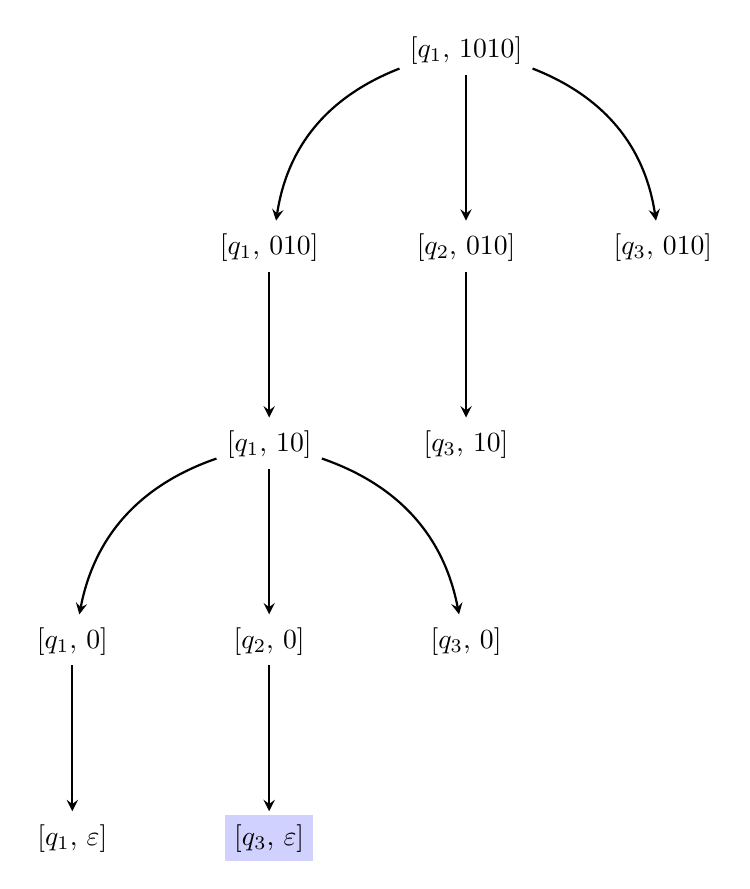
\begin{tikzpicture}[->,>=stealth,shorten >=1pt,auto,node distance=2.5cm,thick,main node/.style={scale=0.9,circle,draw,font=\sffamily\normalsize}]

                \node (1) [] {\ttt{[$q_1$, 1010]}};

                \node (11) [below of=1] {\ttt{[$q_2$, 010]}};
                \node (12) [left of=11] {\ttt{[$q_1$, 010]}};
                \node (13) [right of=11] {\ttt{[$q_3$, 010]}};

                \node (111) [below of=11] {\ttt{[$q_3$, 10]}};
                \node (121) [below of=12] {\ttt{[$q_1$, 10]}};

                \node (1211) [below of=121] {\ttt{[$q_2$, 0]}};
                \node (1212) [left of=1211] {\ttt{[$q_1$, 0]}};
                \node (1213) [right of=1211] {\ttt{[$q_3$, 0]}};

                \node[fill=white!10!blue!20] (12121) [below of=1211] {\ttt{[$q_3$, $\varepsilon$]}};
                \node (12111) [below of=1212] {\ttt{[$q_1$, $\varepsilon$]}};

                \path[every node/.style={font=\sffamily\small}]
                    (1) edge [] (11)
                    (1) edge [bend right] (12)
                    (1) edge [bend left] (13)

                    (11) edge [] (111)
                    (12) edge [] (121)

                    (121) edge [] (1211)
                    (121) edge [bend right] (1212)
                    (121) edge [bend left] (1213)

                    (1211) edge [] (12121)
                    (1212) edge [] (12111)
                 ;
             \end{tikzpicture}
        \end{center}

        \item Poiché esiste un ramo che termina correttamente, l'\NFA descritto accetta la stringa \ttt{w = 1010}
    
    \end{itemize}

    \begin{framedprop}{Stringa accettata in un \NFA}
        Sia $N := (Q, \Sigma, \delta, q_0, F)$ un \NFA. Data una stringa $w := w_0 \ldots w_{k} \in \Sigma^*$, dove $w_0, \ldots, \\ w_k \in \Sigma_{\varepsilon}$, diciamo che $w$ è \textbf{accettata da $N$} se esiste una sequenza di stati $r_0, r_1, \ldots, \\ r_{k+1} \in Q$ tali che:
        \begin{itemize}
            \item $r_0 = q_0$
            \item $\forall i \in [0,k] \;\; r_{i+1} \in \delta(r_i, w_i)$
            \item $r_{k+1} \in F$
        \end{itemize}
    \end{framedprop}

    \subsection{Equivalenza tra \NFA e \DFA}

    \begin{frameddefn}{Classe dei linguaggi riconosciuti da un \DFA}
        Dato un alfabeto $\Sigma$, definiamo come \textbf{classe dei linguaggi di $\Sigma$ riconosciuti da un \DFA} il seguente insieme:
        \[\mathcal{L}(\text{\DFA}) = \{L \subseteq \Sigma^* \mid \exists \; \DFA \; D \text{ t.c } L = L(D)\}\]
    \end{frameddefn}

    \begin{frameddefn}{Classe dei linguaggi riconosciuti da un \NFA}
        Dato un alfabeto $\Sigma$, definiamo come \textbf{classe dei linguaggi di $\Sigma$ riconosciuti da un \NFA} il seguente insieme:
        \[\mathcal{L}(\text{\NFA}) = \{L \subseteq \Sigma^* \mid \exists \; \NFA \; N \text{ t.c } L = L(N)\}\]
    \end{frameddefn}

    \begin{framedthm}[label=NFAeqDFA]{Equivalenza tra \NFA e \DFA}
        Date le due classi dei linguaggi $\mathcal{L}(\text{\DFA})$ e $\mathcal{L}(\text{\NFA})$, si ha che:
        \[\mathcal{L}(\text{\DFA}) = \mathcal{L}(\text{\NFA})\]
    \end{framedthm}

    \proofiff{
        \begin{itemize}
            \item Dato $L \in \mathcal{L}(\text{\DFA})$, sia $D := (Q, \Sigma, \delta, q_0, F)$ il \DFA tale che $L = L(D)$
            \item Poiché il concetto di \NFA è una generalizzazione del concetto di \DFA, ne segue automaticamente che $D$ sia anche un \NFA, implicando che $L \in \mathcal{L}(\text{\NFA})$ e di conseguenza che:
            \[\mathcal{L}(\text{\DFA}) \subseteq \mathcal{L}(\text{\NFA})\]
        \end{itemize}

    }{
        \begin{itemize}
            \item Dato $L \in \mathcal{L}(\text{\NFA})$, sia $N := (Q_N, \Sigma, \delta_{N}, q_{0_N}, F_N)$ il \NFA tale che $L = L(N)$
            \item Consideriamo quindi il \DFA $D := (Q_D, \Sigma, \delta_{D}, q_{0_D}, F_D)$ costruito tramite $N$ stesso:
            \begin{itemize}
                \item $Q_D = \mathcal{P}(Q_N)$
                \item Dato $R \in Q_D$, definiamo l'estensione di $R$ come:
                \[E(R) = \left \{q \in Q_N \mid \exists p \in R \text{ che raggiunge $q$ in $N$ tramite solo $\varepsilon$-archi} \right \}\]
                \item $q_{0_D} = E(\{q_{0_N}\})$
                \item $F_D = \{R \in Q_D \mid R \cap F_N \neq \varnothing\}$
                \item Dati $R \in Q_D$ e $a \in \Sigma$, definiamo $\delta_D$ come:
                \[\delta_D(R, a) = \bigcup_{r \in R} E(\delta_N(r,a))\]
            \end{itemize}
            
            \item A questo punto, per costruzione stessa di $D$ si ha che:
            \[w \in L = L(N) \iff w \in L(D)\]
            implicando dunque che $L \in \mathcal{L}(\text{\DFA})$ e di conseguenza che:
            \[\mathcal{L}(\text{\NFA}) \subseteq \mathcal{L}(\text{\DFA})\]
        \end{itemize}
    }

    \begin{framedobs}{}
        Dato un \NFA $N$, seguendo i passaggi della dimostrazione precedente è possibile definire un \DFA $D$ equivalente ad $N$
    \end{framedobs}


    \textbf{Esempio:}

    \begin{itemize}
        \item Consideriamo ancora il seguente \NFA
        
        \begin{center}
            \begin{tikzpicture}[->,>=stealth,shorten >=1pt,auto,node distance=2.5cm,thick,main node/.style={scale=0.9,circle,draw,font=\sffamily\normalsize}]
                \node[initial,state,accepting] (1) {$q_1$};
                \node[state] (2) [below of=1] {$q_2$};
                \node[state] (3) [right of=1] {$q_3$};
     
                \path[every node/.style={font=\sffamily\small}]
                    (1) edge [bend left] node {$\varepsilon$} (3)
                    (3) edge [bend left] node {\ttt a} (1)
                    (1) edge [bend right] node {\ttt b} (2)
                    (2) edge [loop left] node {\ttt a} (2)
                    (2) edge [bend right] node {\ttt a,b} (3)
                 ;
             \end{tikzpicture}
        \end{center}
        
        \item Definiamo quindi l'insieme degli stati del \DFA equivalente a tale \NFA:
        \[Q_D = \{\varnothing, \{q_1\}, \{q_2\}, \{q_3\}, \{q_1, q_2\}, \{q_2, q_3\}, \{q_1, q_3\}, \{q_1,q_2,q_3\}\} =\]

        \item Per facilitare la lettura, riscriviamo i vari stati con la seguente notazione
        \[Q_D = \{\varnothing, q_1, q_2, q_3, q_{1,2}, q_{2,3}, q_{1,3}, q_{1,2,3}\}\]

        \item A questo punto, poniamo:
        \begin{itemize}
            \item $q_{0_D} = E(\{q_{0_N}\}) = E(\{q_1\}) = \{q_1, q_3\} = q_{1,3}$
            \item $F_D = \{q_1, q_{1,2}, q_{1,3}, q_{1,2,3}\}$
        \end{itemize}

        \newpage

        \item Le transizioni del \DFA corrisponderanno invece a:
        \begin{itemize}
            \item $\delta_D(\{q_1\}, a) = E(\delta_N(q_1,a)) = \varnothing$
            \item $\delta_D(\{q_1\}, b) = E(\delta_N(q_1,b)) = \{q_2\}$
            \item $\delta_D(\{q_2\}, a) = E(\delta_N(q_2,a)) = \{q_2,q_3\}$
            \item $\delta_D(\{q_2\}, b) = E(\delta_N(q_2,b)) = \{q_3\}$
            \item $\delta_D(\{q_1, q_2\}, a) = E(\delta_N(q_1, a)) \cup E(\delta_N(q_2, a)) = \varnothing \cup \{q_2, q_3\} = \{q_2, q_3\}$
            \item $\delta_D(\{q_1, q_2\}, b) = E(\delta_N(q_1, b)) \cup E(\delta_N(q_2, b)) = \{q_2\} \cup \{q_3\} = \{q_2, q_3\}$
            \item $\ldots$
        \end{itemize}

        \item Il \DFA equivalente corrisponde dunque a:
        
        \begin{center}
            \begin{tikzpicture}[->,>=stealth,shorten >=1pt,auto,node distance=2.5cm,thick,main node/.style={scale=0.9,circle,draw,font=\sffamily\normalsize}]
                \node[state] (0) {$\varnothing$};
                \node[state,accepting] (1) [right of=0] {$q_1$};
                \node[state] (2) [right of=1] {$q_2$};
                \node[state,accepting] (12) [right of=2] {$q_{1,2}$};
                \node[state] (3) [below of=0] {$q_3$};
                \node[state,accepting,initial below] (13) [right of=3] {$q_{1,3}$};
                \node[state] (23) [right of=13] {$q_{2,3}$};
                \node[state,accepting] (123) [right of=23] {$q_{1,2,3}$};
     
                \path[every node/.style={font=\sffamily\small}]
                    (0) edge [loop left] node {\ttt a,b} (0)

                    (1) edge [bend right] node [above]{\ttt a} (0)
                    (1) edge [bend left] node {\ttt b} (2)

                    (2) edge [] node {\ttt a} (23)
                    (2) edge [] node[above]{\ttt b} (3)

                    (3) edge [] node {\ttt a} (13)
                    (3) edge [bend left] node {\ttt b} (0)
                    
                    (12) edge [] node[above, anchor=south, yshift=5]{\ttt{a,b}} (23)
                    
                    (23) edge [bend left] node {\ttt a} (123)
                    (23) edge [in=270, out=270] node {\ttt b} (3)
                    
                    (13) edge [loop right] node {\ttt a} (13)
                    (13) edge [in=240, out=30] node {\ttt b} (2)
                    
                    (123) edge [loop right] node {\ttt a} (123)
                    (123) edge [bend left] node {\ttt b} (23)
                 ;
             \end{tikzpicture}
        \end{center}
        
    \end{itemize}


    \begin{frameddefn}{Linguaggi regolari}
        Dato un alfabeto $\Sigma$, definiamo come \textbf{insieme dei linguaggi regolari di $\Sigma$}, indicato con $\mathrm{\REG}$, l'insieme delle classi dei linguaggi riconosciuti da un \DFA:
        \[\mathrm{\REG} := \mathcal{L}(\DFA)\]
    \end{frameddefn}

    \begin{framedobs}{}
        Tramite il teorema dell'\nameref{NFAeqDFA}, si ha che:
        \[\mathrm{\REG} := \mathcal{L}(\DFA) = \mathcal{L}(\NFA)\]
    \end{framedobs}

    \newpage

    \section{Chiusure dei linguaggi regolari}

    \begin{framedthm}[label=UnionREG]{Chiusura dell'unione in $\mathrm{\REG}$}
        L'operatore unione è \textbf{chiuso in $\mathrm{\REG}$}, ossia:
        \[\forall L_1, L_2 \in \mathrm{\REG} \;\; L_1 \cup L_2 \in \mathrm{\REG}\] 
    \end{framedthm}

    \proofenv[Dimostrazione I]{
        \begin{itemize}
            \item Dati $L_1, L_2 \in \mathrm{\REG}$, siano $D_1 = (Q_1, \Sigma, \delta_1, q_1, F_1)$ e $D_2 = (Q_2, \Sigma, \delta_2, q_2, F_2)$ i due \DFA tali che $L_1 = L(D_1)$ e $L_2 = L(D_2)$
            
            \item Definiamo quindi il \DFA $D = (Q, \Sigma, \delta, q_0, F)$ tale che:
            \begin{itemize}
                \item $q_0 = (q_1, q_2)$
                \item $Q = Q_1 \times Q_2$
                \item $F = (F_1 \times Q_2) \cup (Q_1 \times F_2) = \{(r_1, r_2) \mid r_1 \in F_1 \lor r_2 \in F_2\}$
                \item $\forall (r_1, r_2) \in Q, a \in \Sigma$ si ha che:
                \[\delta((r_1,r_2), a) = (\delta_1(r_1, a), \delta_2(r_2, a))\]
            \end{itemize}

            \item A questo punto, per costruzione stessa di $D$ ne segue che:
            \[w \in L_1 \cup L_2 \iff w \in L(D)\]
            dunque che $L_1 \cup L_2 = L(D)\in \mathrm{\REG}$
        \end{itemize}
    }

    \proofenv[Dimostrazione II]{
        \begin{itemize}
            \item Dati $L_1, L_2 \in \mathrm{\REG}$, siano $N_1 = (Q_1, \Sigma, \delta_1, q_1, F_1)$ e $N_2 = (Q_2, \Sigma, \delta_2, q_2, F_2)$ i due \NFA tali che $L_1 = L(N_1)$ e $L_2 = L(N_2)$
            \item Definiamo quindi il \NFA $N = (Q, \Sigma, \delta, q_0, F)$ tale che:
            \begin{itemize}
                \item $q_0$ è un nuovo stato iniziale aggiunto
                \item $Q = Q_1 \cup Q_2 \cup \{q_0\}$
                \item $F = F_1 \cup F_2$
                \item $\forall q \in Q, a \in \Sigma$ si ha che:
                \[\delta(q, a) = \soe{ll}{
                    \delta_1(q, a) & \text{ se } q \in Q_1 \\
                    \delta_2(q, a) & \text{ se } q \in Q_2 \\
                    \{q_1, q_2\} & \text{ se } q = q_0 \land a = \varepsilon \\
                    \varnothing & \text{ se } q = q_0 \land a \neq \varepsilon \\
                }\]
            \end{itemize}

            \item A questo punto, per costruzione stessa di $N$ ne segue che:
            \[w \in L_1 \cup L_2 \iff w \in L(N)\]
            dunque che $L_1 \cup L_2 = L(N)\in \mathrm{\REG}$
        \end{itemize}
    }

    \begin{center}
        \includegraphics[scale=0.475]{images/union_proof.png}

        \textit{Rappresentazione grafica della dimostrazione}
    \end{center}

    \begin{framedthm}[label=InterREG]{Chiusura dell'intersezione in $\mathrm{\REG}$}
        L'operatore intersezione è \textbf{chiuso in $\mathrm{\REG}$}, ossia:
        \[\forall L_1, L_2 \in \mathrm{\REG} \;\; L_1 \cap L_2 \in \mathrm{\REG}\] 
    \end{framedthm}

    \proofenv{
        \begin{itemize}
            \item Dati $L_1, L_2 \in \mathrm{\REG}$, siano $D_1 = (Q_1, \Sigma, \delta_1, q_1, F_1)$ e $D_2 = (Q_2, \Sigma, \delta_2, q_2, F_2)$ i due \DFA tali che $L_1 = L(D_1)$ e $L_2 = L(D_2)$
            \item Definiamo quindi il \DFA $D = (Q, \Sigma, \delta, q_0, F)$ tale che:
            \begin{itemize}
                \item $q_0 = (q_1, q_2)$
                \item $Q = Q_1 \times Q_2$
                \item $F = F_1 \times F_2 = \{(r_1, r_2) \mid r_1 \in F_1 \land r_2 \in F_2\}$
                \item $\forall (r_1, r_2) \in Q, a \in \Sigma$ si ha che:
                \[\delta((r_1,r_2), a) = (\delta_1(r_1, a), \delta_2(r_2, a))\]
            \end{itemize}

            \item A questo punto, per costruzione stessa di $D$ ne segue che:
            \[w \in L_1 \cap L_2 \iff w \in L(D)\]
            dunque che $L_1 \cap L_2 = L(D)\in \mathrm{\REG}$
        \end{itemize}
    }

    \newpage

    \begin{framedthm}[label=CompREG]{Chiusura del complemento in $\mathrm{\REG}$}
        L'operatore complemento è \textbf{chiuso in $\mathrm{\REG}$}, ossia:
        \[\forall L \in \mathrm{\REG} \;\; \overline{L} \in \mathrm{\REG}\] 
    \end{framedthm}

    \proofenv{
        \begin{itemize}
            \item Dato $L \in \mathrm{\REG}$, sia $D = (Q, \Sigma, \delta, q_0, F)$ il \DFA tale che $L = L(D)$
            \item Definiamo quindi il \DFA $D' = (Q, \Sigma, \delta, q_0, Q-F)$, dunque il \DFA uguale a $D$ ma i cui stati accettanti sono invertiti. Per costruzione stessa di $D'$ ne segue che:
            \[w \in L \iff w \notin L(D')\]
            dunque che $\overline{L} = L(D')\in \mathrm{\REG}$
        \end{itemize}
    }

    \begin{framedthm}[label=ConcatREG]{Chiusura della concatenazione in $\mathrm{\REG}$}
        L'operatore concatenazione è \textbf{chiuso in $\mathrm{\REG}$}, ossia:
        \[\forall L_1, L_2 \in \mathrm{\REG} \;\; L_1 \circ L_2 \in \mathrm{\REG}\] 
    \end{framedthm}

    \proofenv{
        \begin{itemize}
            \item Dati $L_1, L_2 \in \mathrm{\REG}$, siano $N_1 = (Q_1, \Sigma, \delta_1, q_1, F_1)$ e $N_2 = (Q_2, \Sigma, \delta_2, q_2, F_2)$ i due \NFA tali che $L_1 = L(N_1)$ e $L_2 = L(N_2)$
            \item Definiamo quindi il \NFA $N = (Q, \Sigma, \delta, q_0, F)$ tale che:
            \begin{itemize}
                \item $q_0 = q_1$
                \item $Q = Q_1 \cup Q_2$
                \item $F = F_2$
                \item $\forall q \in Q, a \in \Sigma$ si ha che:
                \[\delta(q,a) = \soe{ll}{
                    \delta_1(q, a) & \text{ se } q \in Q_1-F_1 \\
                    \delta_1(q, a) & \text{ se } q \in F_1 \land a \neq \varepsilon \\
                    \delta_1(q, a) \cup \{q_2\} & \text{ se } q \in F_1 \land a = \varepsilon \\
                    \delta_2(q, a) & \text{ se } q \in Q_2
                }\]
            \end{itemize}

            \item A questo punto, per costruzione stessa di $N$ ne segue che:
            \[w \in L_1 \circ L_2 \iff w \in L(N)\]
            dunque che $L_1 \circ L_2 = L(N)\in \mathrm{\REG}$
        \end{itemize}
    }

    \begin{center}
        \includegraphics[scale=0.5]{images/concat_proof.png}

        \textit{Rappresentazione grafica della dimostrazione}
    \end{center}

    \quad

    \begin{framedcor}[label=PowerREG]{Chiusura della potenza in $\mathrm{\REG}$}
        L'operatore potenza è \textbf{chiuso in $\mathrm{\REG}$}, ossia:
        \[\forall L \in \mathrm{\REG}, n \in \N \;\; L^n \in \mathrm{\REG}\] 
    \end{framedcor}

    \begin{framedthm}[label=StarREG]{Chiusura di star in $\mathrm{\REG}$}
        L'operatore star è \textbf{chiuso in $\mathrm{\REG}$}, ossia:
        \[\forall L \in \mathrm{\REG} \;\; L^* \in \mathrm{\REG}\] 
    \end{framedthm}

    \proofenv{
        \begin{itemize}
            \item Dato $L \in \mathrm{\REG}$, sia $N = (Q, \Sigma, \delta, q_0, F)$ il \NFA tale che $L = L(N)$
            \item Definiamo quindi il \DFA $N' = (Q', \Sigma, \delta', q_{0*}, F')$ tale che:
            \begin{itemize}
                \item $q_{0*}$ è un nuovo stato iniziale aggiunto
                \item $Q' = Q \cup \{q_{0*}\}$
                \item $F' = F \cup \{q_{0*}\}$
                \item $\forall q \in Q', a \in \Sigma$ si ha che:
                \[\delta'(q,a) = \soe{ll}{
                    \delta(q, a) & \text{ se } q \in Q-F \\
                    \delta(q, a) & \text{ se } q \in F \land a \neq \varepsilon \\
                    \delta(q, a) \cup \{q_0\} & \text{ se } q \in F \land a = \varepsilon \\
                    \{q_0\} & \text{ se }q = q_{0*} \land a = \varepsilon \\
                    \varnothing & \text{ se }q = q_{0*} \land a \neq \varepsilon \\
                }\]
            \end{itemize}
            \item A questo punto, per costruzione stessa di $N'$ ne segue che:
            \[w \in L^* \iff w \in L(N')\]
            dunque che $L^* = L(N')\in \mathrm{\REG}$
        \end{itemize}
    }

    \begin{center}
        \includegraphics[scale=0.55]{images/star_proof.png}

        \textit{Rappresentazione grafica della dimostrazione}
    \end{center}

    \begin{framedcor}[label=StarREG]{Chiusura di plus in $\mathrm{\REG}$}
        L'operatore plus è \textbf{chiuso in $\mathrm{\REG}$}, ossia:
        \[\forall L \in \mathrm{\REG} \;\; L^+ \in \mathrm{\REG}\] 
    \end{framedcor}
    \proofenv{
        \begin{itemize}
            \item Analoga a quella dell'operatore star, rimuovendo tuttavia lo stato iniziale dall'insieme degli stati accettanti
        \end{itemize}
    }

    \newpage

    \section{Espressioni regolari}

    \begin{frameddefn}{Espressione regolare}
        Dato un alfabeto $\Sigma$, definiamo come \textbf{espressione regolare di $\Sigma$} una stringa $R$ rappresentante un linguaggio $L(R) \subseteq \Sigma^*$. In altre parole, ogni espressione regolare $R$ rappresenta in realtà il linguaggio $L(R)$ ad essa associata.
        
        In particolare, definiamo l'\textbf{insieme delle espressioni regolari di $\Sigma$}, indicato con $\mathrm{re}(\Sigma)$, come:
        \begin{itemize}
            \item $\varnothing \in \mathrm{re}(\Sigma)$
            \item $\varepsilon \in \mathrm{re}(\Sigma)$
            \item $a \in \mathrm{re}(\Sigma)$, dove $a \in \Sigma$
            \item $R_1, R_2 \in \mathrm{re}(\Sigma) \implies R_1 \cup R_2 \in \mathrm{re}(\Sigma)$
            \item $R_1, R_2 \in \mathrm{re}(\Sigma) \implies R_1 \circ R_2 \in \mathrm{re}(\Sigma)$
            \item $R \in \mathrm{re}(\Sigma) \implies R^* \in \mathrm{re}(\Sigma)$
            \item $R \in \mathrm{re}(\Sigma) \implies R^+ \in \mathrm{re}(\Sigma)$
        \end{itemize}
    \end{frameddefn}

    \begin{framedobs}{}
        Data un'espressione regolare $R \in \mathrm{re}(R)$, si ha che:
        \begin{itemize}
            \item $R = \varnothing \in \mathrm{re}(\Sigma) \implies L(R) = \varnothing$
            \item $R = \varepsilon \in \mathrm{re}(\Sigma) \implies L(R) = \{\varepsilon\}$
            \item $R = a \in \mathrm{re}(\Sigma), a \in \Sigma \implies L(R) = \{a\}$
            \item $R = R_1 \cup R_2 \in \mathrm{re}(\Sigma) \implies L(R) = L(R_1) \cup L(R_2) $
            \item $R = R_1 \circ R_2 \in \mathrm{re}(\Sigma) \implies L(R) =  L(R_1) \circ L(R_2) $
            \item $R = R_1^* \in \mathrm{re}(\Sigma) \implies L(R) = L(R_1)^* $
            \item $R = R_1^+ \in \mathrm{re}(\Sigma) \implies L(R) = L(R_1)^+ $
        \end{itemize}
    \end{framedobs}

    \textbf{Esempi:}

    \begin{enumerate}
        \item $0 \cup 1$ rappresenta il linguaggio $\{0\} \cup \{1\} = \{0,1\}$
        \item $0^*10^*$ rappresenta il linguaggio $\{0\}^* \circ \{1\} \circ \{0\}^* = \{ x1y \mid x,y \in \{0\}^*\}$
        \item $\Sigma^*1\Sigma^*$ rappresenta il linguaggio $\Sigma^* \circ \{1\} \circ \Sigma^* = \{ x1y \mid x,y \in \Sigma^*\}$
        \item $(0 \cup 1000)^*$ rappresenta il linguaggio $(\{0\} \cup \{1000\})^* = \{0, 1000\}^*$
        \item $\varnothing^*$ rappresenta il linguaggio $\varnothing^* = \{\varepsilon\}$ (ricordiamo che per definizione stessa si ha che $\forall L \subseteq \Sigma^* \;\; L^0 = \{\varepsilon\}$)
        \item $0^*\varnothing$ rappresenta il linguaggio $\{0\}^* \circ \varnothing = \varnothing$
        \item $(0 \cup \varepsilon)(1 \cup \varepsilon)$ rappresenta il linguaggio $\{\varnothing, 0, 1, 01\}$
        \item $\Sigma^+$ equivale all'espressione $\Sigma \Sigma^*$
    \end{enumerate}


    \begin{frameddefn}{Classe dei linguaggi descritti da esp. reg.}
        Dato un alfabeto $\Sigma$, definiamo come \textbf{classe dei linguaggi di $\Sigma$ descritti da un'espressione regolare} il seguente insieme:
        \[\mathcal{L}(\mathrm{re}) = \{L \subseteq \Sigma^* \mid \exists R \in \mathrm{re}(\Sigma) \text{ t.c. } L = L(R)\}\]
    \end{frameddefn}

    \begin{framedlem}[label=REtoNFA]{Conversione da espressione regolare a \NFA}
        Date le due classi dei linguaggi $\mathcal{L}(\mathrm{re})$ e $\mathcal{L}(\NFA)$, si ha che:
        \[\mathcal{L}(\mathrm{re}) \subseteq \mathcal{L}(\NFA)\]
    \end{framedlem}

    \proofind{
        \begin{itemize}
            \item[] Procediamo per induzione strutturale, ossia dimostrando che se per ogni sotto-componente vale una determinata proprietà allora essa varrà anche per ogni componente formato da tali sotto-componenti 
        \end{itemize}

    }{
        \begin{itemize}
            \item Se $R = \varnothing \in \mathrm{re}(\Sigma)$, definiamo il \NFA $N_{\varnothing} = (\{q_0\}, \Sigma, \delta, q_0, \varnothing)$, ossia:

            \begin{center}
                \begin{tikzpicture}[->,>=stealth,shorten >=1pt,auto,node distance=2.5cm,thick,main node/.style={scale=0.9,circle,draw,font=\sffamily\normalsize}]
                    \node[state,initial] (0) {$q_0$};
        
                    \path[every node/.style={font=\sffamily\small}]
                    ;
                \end{tikzpicture}
            \end{center}
            per cui si ha che $w \in L(R) \iff w \in L(N_{\varnothing}) $ dunque $ L(R) = L(N_{\varnothing}) \in \mathcal{L}(\NFA) $

            \item Se $R = \varepsilon \in \mathrm{re}(\Sigma)$, definiamo il \NFA $N_{\varepsilon} = (\{q_0\}, \Sigma, \delta, q_0, \{q_0\})$, ossia:
            \begin{center}
                \begin{tikzpicture}[->,>=stealth,shorten >=1pt,auto,node distance=2.5cm,thick,main node/.style={scale=0.9,circle,draw,font=\sffamily\normalsize}]
                    \node[state,initial,accepting] (0) {$q_0$};
        
                    \path[every node/.style={font=\sffamily\small}]
                    ;
                \end{tikzpicture}
            \end{center}
            per cui si ha che $w \in L(R) \iff w \in L(N_{\varepsilon})$ dunque $ L(R) = L(N_{\varepsilon}) \in \mathcal{L}(\NFA) $

            \item Se $R = a  \in \mathrm{re}(\Sigma)$ con $a \in \Sigma$, definiamo il \NFA $N_a = (\{q_0, q_1\}, \Sigma, \delta, q_0, \{q_1\})$ dove per $\delta$ è definita solo la coppia $\delta(q_0, a) = q_1$, ossia:
            \begin{center}
                \begin{tikzpicture}[->,>=stealth,shorten >=1pt,auto,node distance=2.5cm,thick,main node/.style={scale=0.9,circle,draw,font=\sffamily\normalsize}]
                    \node[state,initial] (0) {$q_0$};
                    \node[state,accepting] (1) [right of=0]{$q_1$};
        
                    \path[every node/.style={font=\sffamily\small}]
                        (0) edge node{\ttt a} (1)
                    ;
                \end{tikzpicture}
            \end{center}
            per cui si ha che $w \in L(R) \iff w \in L(N_a)$ dunque $L(R) = L(N_a) \in \mathcal{L}(\NFA) $
        \end{itemize}

        \newpage
    }{
        \begin{itemize}
            \item Date $R_1, R_2 \in \mathrm{re}(\Sigma)$, assumiamo che $\exists \text{ \NFA } N_1, N_2 \mid L(R_1) = L(N_1), L(R_2) = L(N_2)$, dunque che $L(R_1), L(R_2) \in  \mathcal{L}(\NFA) $
        \end{itemize}
    }{
        \begin{itemize}
            \item Se $R = R_1 \cup R_2$, tramite la \nameref{UnionREG}, otteniamo che:
            \[L(R) = L(R_1) \cup L(R_2) = L(N_1) \cup L(N_2) \in  \mathrm{\REG} = \mathcal{L}(\NFA) \]
            \item Se $R = R_1 \circ R_2$, tramite la \nameref{ConcatREG}, otteniamo che:
            \[L(R) = L(R_1) \circ L(R_2) = L(N_1) \circ L(N_2) \in  \mathrm{\REG} = \mathcal{L}(\NFA) \]
            \item Se $R = R_1^*$, tramite la \nameref{StarREG}, otteniamo che:
            \[L(R) = L(R_1)^* = L(N_1)^* \in  \mathrm{\REG} = \mathcal{L}(\NFA) \]
        \end{itemize}
    }

    \textbf{Esempio:}

    \begin{itemize}
        \item Consideriamo l'espressione regolare $(a \cup ab)^*$
        \item Costruiamo il \NFA corrispondente a tale espressione partendo dai suoi sotto-componenti
        
        \begin{center}
            \begin{tabular}{rll}

                $a$ & $\; \implies \;$ &

                \begin{tabular}{c}
                    \begin{tikzpicture}[->,>=stealth,shorten >=1pt,auto,node distance=2.5cm,thick,main node/.style={scale=0.9,circle,draw,font=\sffamily\normalsize}, every node/.style={scale=0.75}]
                        \node[state,initial] (0) {};
                        \node[state,accepting] (1) [right of=0]{};
            
                        \path[every node/.style={font=\sffamily\small}]
                            (0) edge node{\ttt a} (1)
                        ;
                    \end{tikzpicture}
                \end{tabular}
                \\\\

                $b$ & $\; \implies \;$ &

                \begin{tabular}{c}
                    \begin{tikzpicture}[->,>=stealth,shorten >=1pt,auto,node distance=2.5cm,thick,main node/.style={scale=0.9,circle,draw,font=\sffamily\normalsize}, every node/.style={scale=0.75}]
                        \node[state,initial] (0) {};
                        \node[state,accepting] (1) [right of=0]{};
            
                        \path[every node/.style={font=\sffamily\small}]
                            (0) edge node{\ttt b} (1)
                        ;
                    \end{tikzpicture}
                \end{tabular}
                \\\\

                $ab$ & $\; \implies \;$ &

                \begin{tabular}{c}
                    \begin{tikzpicture}[->,>=stealth,shorten >=1pt,auto,node distance=2.5cm,thick,main node/.style={scale=0.9,circle,draw,font=\sffamily\normalsize}, every node/.style={scale=0.75}]
                        \node[state,initial] (0) {};
                        \node[state] (1) [right of=0]{};
                        \node[state] (2) [right of=1]{};
                        \node[state,accepting] (3) [right of=2]{};
            
                        \path[every node/.style={font=\sffamily\small}]
                            (0) edge node{\ttt a} (1)
                            (1) edge node{$\varepsilon$} (2)
                            (2) edge node{\ttt b} (3)
                        ;
                    \end{tikzpicture}
                \end{tabular}
                \\\\

                $(a \cup ab)$ & $\; \implies \;$ &

                \begin{tabular}{c}
                    \begin{tikzpicture}[->,>=stealth,shorten >=1pt,auto,node distance=2.5cm,thick,main node/.style={scale=0.9,circle,draw,font=\sffamily\normalsize}, every node/.style={scale=0.75}]
                        \node[state,initial] (0) {};
                        \node[state] (1a) [right of=0]{};
                        \node[state, accepting] (2a) [right of=1a]{};

                        \node[state] (1ab) [below right of=0]{};
                        \node[state] (2ab) [right of=1ab]{};
                        \node[state] (3ab) [right of=2ab]{};
                        \node[state,accepting] (4ab) [right of=3ab]{};
            
                        \path[every node/.style={font=\sffamily\small}]
                            (0) edge node{$\varepsilon$} (1a)
                            (1a) edge node{\ttt a} (2a)

                            (0) edge[bend right] node{$\varepsilon$} (1ab)
                            (1ab) edge node{\ttt a} (2ab)
                            (2ab) edge node{$\varepsilon$} (3ab)
                            (3ab) edge node{\ttt b} (4ab)
                        ;
                    \end{tikzpicture}
                \end{tabular}
            \end{tabular}
        \end{center}

        \begin{center}
            \begin{tabular}{lll}

                $(a \cup ab)^*$ & $\; \implies \;$ &

                \begin{tabular}{c}
                    \begin{tikzpicture}[->,>=stealth,shorten >=1pt,auto,node distance=2.5cm,thick,main node/.style={scale=0.9,circle,draw,font=\sffamily\normalsize}, every node/.style={scale=0.75}]
                        \node[state,initial,accepting] (-1) {};
                        \node[state] (0)[right of=-1] {};
                        \node[state] (1a) [right of=0]{};
                        \node[state, accepting] (2a) [right of=1a]{};

                        \node[state] (1ab) [below right of=0]{};
                        \node[state] (2ab) [right of=1ab]{};
                        \node[state] (3ab) [right of=2ab]{};
                        \node[state,accepting] (4ab) [right of=3ab]{};
            
                        \path[every node/.style={font=\sffamily\small}]
                            (-1) edge node{$\varepsilon$} (0)

                            (0) edge node{$\varepsilon$} (1a)
                            (1a) edge node{\ttt a} (2a)
                            (2a) edge[in=45, out=135] node{$\varepsilon$} (0)

                            (0) edge[bend right] node{$\varepsilon$} (1ab)
                            (1ab) edge node{\ttt a} (2ab)
                            (2ab) edge node{$\varepsilon$} (3ab)
                            (3ab) edge node{\ttt b} (4ab)
                            (4ab) edge[in=270, out=225] node{$\varepsilon$} (0)
                        ;
                    \end{tikzpicture}
                \end{tabular}
            \end{tabular}
        \end{center}
    \end{itemize}

    \newpage

    \subsection{\NFA generalizzati}

    \begin{frameddefn}{Generalized \NFA (\GNFA)}
        Un \textbf{Generalized \NFA (\GNFA)} è una quintupla $(Q, \Sigma, \delta, q_{\mathrm{start}}, q_{\mathrm{accept}})$ dove:
        \begin{itemize}
            \item $Q$ è l'\textbf{insieme finito degli stati} dell'automa dove $\abs{Q} \geq 2$
            \item $\Sigma$ è l'\textbf{alfabeto} dell'automa
            \item $q_{\mathrm{start}} \in Q$ è lo \textbf{stato iniziale} dell'automa
            \item $q_{\mathrm{accept}} \in Q$ è l'\textbf{unico stato accettante} dell'automa
            \item $\func{\delta}{(Q-\{q_{\mathrm{accept}}\}) \times (Q-\{q_{\mathrm{start}}\})}{\mathrm{re}(\Sigma)}$ è la \textbf{funzione di transizione degli stati} dell'automa, implicando che:
            \begin{itemize}
                \item Lo stato $q_{\mathrm{start}}$ abbia solo transizioni \textbf{uscenti}
                \item Lo stato $q_{\mathrm{accept}}$ abbia solo transizioni \textbf{entranti}
                \item Tra \textbf{tutte le possibili coppie di stati} $q, q' \in Q$ (incluso il caso in cui $q = q'$) vi sia una transizione $q \to q'$ ed una transizione $q' \to q$
                \item Le "etichette" delle transizioni sono delle \textbf{espressioni regolari }
            \end{itemize}
        \end{itemize}
    \end{frameddefn}

    \textbf{Esempio:}

    \begin{center}
        \begin{tikzpicture}[->,>=stealth,shorten >=1pt,auto,node distance=3.5cm,thick,main node/.style={scale=0.9,circle,draw,font=\sffamily\normalsize}]
            \node[state,initial] (0) {$q_{\mathrm{start}}$};
            \node[state] (1) [right of=0]{$q_1$};
            \node[state] (2) [above of=1]{$q_2$};
            \node[state,accepting] (3) [right of=1]{$q_{\mathrm{accept}}$};

            \path[every node/.style={font=\sffamily\small}]
            (0) edge[] node{$\varnothing$} (1)
            (0) edge[bend left] node{\ttt{ab$^*$}} (2)
            (0) edge[in=240, out=300] node{\ttt{b}} (3)

            (1) edge[loop below] node{\ttt{ab}} (1)
            (1) edge[bend left] node{\ttt{(aa)}$^*$} (2)
            (1) edge[] node{\ttt{b$^*$}} (3)

            (2) edge[bend left] node{\ttt{a$^*$}} (1)
            (2) edge[loop below] node{\ttt{(aa)}$^*$} (2)
            (2) edge[bend left] node{\ttt{ab$\,\cup\,$ba}} (3)
            ;
        \end{tikzpicture}
    \end{center}

    \begin{framedobs}{}
        In un \GNFA, il risultato $\delta(q,q')=R$ può essere interpretato come "l'espressione regolare che effettua la transizione da $q$ a $q'$ è $R$". Di conseguenza, possiamo immaginare un \GNFA come un \NFA che legga la stringa in input \textbf{blocco per blocco}
    \end{framedobs}

    \begin{framedprop}{Stringa accettata in un \GNFA}
        Sia $G := (Q, \Sigma, \delta, q_{\mathrm{start}}, q_{\mathrm{accept}})$ un \GNFA. Data una stringa $w := w_0 \ldots w_{k} \in \Sigma^*$, dove $w_0, \ldots, w_k \in \Sigma^*$ (ossia sono delle sottostringhe), diciamo che $w$ è \textbf{accettata da $G$} se esiste una sequenza di stati $r_0, r_1, \ldots, r_{k+1} \in Q$ tali che:
        \begin{itemize}
            \item $r_0 = q_{\mathrm{start}}$
            \item $\forall i \in [0,k] \;\; w_i \in L(\delta(r_i, r_{i+1}))$
            \item $r_{k+1} = q_{\mathrm{accept}}$
        \end{itemize}
    \end{framedprop}

    \textbf{Esempio:}

    \begin{itemize}
        \item Il \GNFA dell'esempio precedente accetta la stringa \ttt{ababaaaba}, poiché:
        \begin{itemize}
            \item $\delta(q_{\mathrm{start}}, q_1) = \ttt{ab}^*$, dunque viene letta in blocco la sottostringa \ttt{abab}
            \item $\delta(q_1, q_1) = \ttt{aa}^*$, dunque viene letta in blocco la sottostringa \ttt{aa}
            \item $\delta(q_1, q_{\mathrm{accept}}) = \ttt{ab}\,\cup\,\ttt{ba}$, dunque viene letta in blocco la sottostringa \ttt{ba}
        \end{itemize}
    \end{itemize}

    \begin{framedcor}{}
        Una transizione con "etichetta" pari a $\varnothing$ è una \textbf{transizione inutilizzabile} in quanto $L(\varnothing) = \varnothing$
    \end{framedcor}

    \begin{frameddefn}{Classe dei linguaggi riconosciuti da un \GNFA}
        Dato un alfabeto $\Sigma$, definiamo come \textbf{classe dei linguaggi di $\Sigma$ riconosciuti da un \GNFA} il seguente insieme:
        \[\mathcal{L}(\text{\GNFA}) = \{L \subseteq \Sigma^* \mid \exists \; \GNFA \; G \text{ t.c } L = L(G)\}\]
    \end{frameddefn}

    \begin{framedlem}[label=DFAtoGNFA]{Conversione da \DFA a \GNFA}
        Date le due classi dei linguaggi $\mathcal{L}(\DFA)$ e $\mathcal{L}(\GNFA)$, si ha che:
        \[\mathcal{L}(\DFA) \subseteq \mathcal{L}(\GNFA)\]
    \end{framedlem}

    \proofenv{
        \begin{itemize}
            \item Dato $L \in \mathcal{L}(\DFA)$, sia $D := (Q, \Sigma, \delta, q_0, F)$ il \DFA tale che $L(D) = L$
        
            \item Consideriamo quindi il \GNFA $G := (Q', \Sigma, \delta', q_{\mathrm{start}}, q_{\mathrm{accept}})$ costruito tramite $D$ stesso:
            \begin{itemize}
                \item $Q' = Q \cup \{q_{\mathrm{start}}, q_{\mathrm{accept}}\}$
                \item $\delta'(q_{\mathrm{start}}, q_0) = \varepsilon$
                \item $\forall q \in F \;\; \delta'(q, q_{\mathrm{accept}}) = \varepsilon$
                \item Per ogni transizione con etichetta multipla in $D$, in $G$ esiste una transizione equivalente con etichetta corrispondente all'unione di tali etichette multiple
                \item Per ogni coppia di stati per cui non esiste una transizione entrante o uscente in $D$, viene aggiunta una transizione con etichetta $\varnothing$
            \end{itemize}

            \item A questo punto, per costruzione stessa di $G$ si ha che:
            \[w \in L = L(D) \implies L(G)\]
            implicando dunque che $L(D) \in \mathcal{L}(\DFA)$ e di conseguenza che:
            \[\mathcal{L}(\DFA) \subseteq \mathcal{L}(\GNFA)\]
        \end{itemize}
    }

    \textbf{Esempio:}

    \begin{itemize}
        \item Consideriamo il seguente \DFA:
        
        \begin{center}
            \begin{tikzpicture}[->,>=stealth,shorten >=1pt,auto,node distance=2.5cm,thick,main node/.style={scale=0.9,circle,draw,font=\sffamily\normalsize}]
                \node[state,initial] (0) {$q_0$};
                \node[state,accepting] (1) [right of=0]{$q_1$};

                \path[every node/.style={font=\sffamily\small}]
                (0) edge[] node{\ttt{2}} (1)
                (0) edge[loop above] node{\ttt{0,1}} (0)
                (1) edge[loop above] node{\ttt{0,1}} (1)
                ;
            \end{tikzpicture}
        \end{center}

        \item Il suo \GNFA equivalente corrisponde a:
        
        \begin{center}
            \begin{tikzpicture}[->,>=stealth,shorten >=1pt,auto,node distance=3cm,thick,main node/.style={scale=0.9,circle,draw,font=\sffamily\normalsize}]
                \node[state,initial] (s) {$q_{\mathrm{start}}$};
                \node[state] (0) [right of=s]{$q_0$};
                \node[state] (1) [right of=0]{$q_1$};
                \node[state,accepting] (a) [right of=1]{$q_{\mathrm{accept}}$};

                \path[every node/.style={font=\sffamily\small}]
                (s) edge[] node{$\varepsilon$} (0)
                (s) edge[in=270, out=270] node{$\varnothing$} (1)
                (s) edge[in=270, out=270] node{$\varnothing$} (a)

                (0) edge[loop above] node{\ttt{0$\,\cup\,$1}} (0)
                (0) edge[bend left] node{\ttt{2}} (1)
                (0) edge[in=270, out=270] node{$\varnothing$} (a)

                (1) edge[loop above] node{\ttt{0$\,\cup\,$1}} (1)
                (1) edge[bend left] node{$\varnothing$} (0)
                (1) edge[] node{$\varepsilon$} (a)

                ;
            \end{tikzpicture}
        \end{center}
    \end{itemize}

    \newpage

    \begin{framedalgo}{Riduzione minimale di un \GNFA}
        Dato un \GNFA $G = (Q, \Sigma, \delta, q_{\mathrm{start}}, q_{\mathrm{accept}})$, il seguente algoritmo restituisce un \GNFA $G'$ avente solo due stati e tale che $L(G) = L(G')$ :

        \begin{algorithmic}
            \Function{reduceGNFA}{$G$}
                \If{$|Q| == 2$}
                \State \textbf{return} $G$
                \ElsIf{$|Q| > 2$}
                    \State $q := q \in Q - \{q_{\mathrm{start}}, q_{\mathrm{accept}}\}$
                    \State $Q' := Q - \{q\}$
                    \For{$q_i \in Q' - \{q_{\mathrm{accept}}\}$}
                        \For{$q_j \in Q' - \{q_{\mathrm{start}}\}$}
                            \State $\delta'(q_i, q_j) := \delta(q_i, q)\delta(q, q)^* \delta(q, q_j) \cup \delta(q_i, q_j)$
                        \EndFor
                    \EndFor
                    
                    \State $G' := (Q', \Sigma, \delta', q_{\mathrm{start}}, q_{\mathrm{accept}})$
                    \State \textbf{return} $\ttt{reduceGNFA}(G')$
                \EndIf
            \EndFunction
        \end{algorithmic}
    \end{framedalgo}

    \proofind{

        Siano $G_0, \ldots, G_n$ i vari \GNFA prodotti dalla ricorsione dell'algoritmo, implicando che $G_0 = G$ e che $G_n$ sia l'output. Procediamo per induzione  sul numero $k \in \N$ di riduzioni effettuate, mostrando che $L(G) = L(G_0) = \ldots = L(G_n)$
    }{
        \begin{itemize}
            \item Se $k = 0$, allora $G_0 = G$, dunque $L(G) = L(G_0)$
        \end{itemize}
    }{
        \begin{itemize}
            \item Dato $k \in \N$, assumiamo che per il \GNFA $G_k := (Q, \Sigma, \delta, q_{\mathrm{start}}, q_{\mathrm{accept}})$ si abbia che $L(G) = L(G_k)$
        \end{itemize}
    }{
        \begin{itemize}
            \item Consideriamo quindi il \GNFA $G_{k+1} := (Q', \Sigma, \delta, q_{\mathrm{start}}, q_{\mathrm{accept}})$ ottenuto rimuovendo uno stato $q \in Q$ (dunque $Q' = Q-\{q\}$) e ponendo
            \[\delta'(q_i, q_j) := \delta(q_i, q)\delta(q, q)^* \delta(q, q_j) \cup \delta(q_i, q_j)\]
            per ogni $q_i \in Q' - \{q_{\mathrm{accept}}\}, q_j \in Q' - \{q_{\mathrm{start}}\}$
            \item Data una stringa $w := w_0 \ldots w_m \in L(G_k)$, dove $w_0, \ldots, w_m \in \Sigma^*$, esiste una sequenza di stati $q_0, \ldots, q_m \in Q$ tali che:
            \begin{itemize}
                \item $q_0 = q_{\mathrm{start}}$ e $q_m = q_{\mathrm{accept}}$
                \item $\forall i \in [0,m-1] \;\; w_i \in L(\delta(q_i, q_{i+1}))$
            \end{itemize}
            \item A questo punto, consideriamo la costruzione della funzione $\delta'$:
            \[\delta'(q_i, q_j) = \delta(q_i, q)\delta(q, q)^* \delta(q, q_j) \cup \delta(q_i, q_j)\]
            \begin{itemize}
                \item Se $q \notin \{q_0, \ldots, q_m\}$, allora tramite l'unione si ha che $w_i \in L(\delta(q_i, q_j)) \implies w \in L(\delta'(q_i, q_j))$, dunque tutte le possibili sottostringhe passanti per le transizioni dirette da $q_i$ a $q_j$ vengono riconosciute
                \item Se $q \in \{q_0, \ldots, q_m\}$, allora la concatenazione $\delta(q_i, q)\delta(q, q)^* \delta(q, q_j)$ permette il riconoscimento di tutti i cammini da $q_i$ a $q_j$ passanti per $q$, implicando che $w \in L(\delta'(q_i, q_j))$
            \end{itemize}

            \item Viceversa, poiché ogni $\delta'(q_i, q_j)$ è definito come la combinazione di tutti i cammini possibili da $q_i$ a $q_j$ (dunque passando per $q$ o non), ne segue automaticamente che $w \in L(G_{k+1}) \implies w \in L(G_k)$
            
            \item Esprimendo il tutto graficamente, risulta evidente che le seguenti transizioni siano del tutto equivalenti:

            \begin{center}
                \begin{tabular}{ccc}
                    \begin{tabular}{c}
                        \begin{tikzpicture}[->,>=stealth,shorten >=1pt,auto,node distance=3cm,thick,main node/.style={scale=0.9,circle,draw,font=\sffamily\normalsize}]
                            \node[state] (0) []{$q_i$};
                            \node[state] (1) [below right of=0]{$q$};
                            \node[state] (2) [above right of=1]{$q_j$};

                            \path[every node/.style={font=\sffamily\small}]
                            (0) edge[bend left] node{$R_4$} (2)
                            (0) edge[bend right] node{$R_1$} (1)
                            (1) edge[loop below] node{$R_2$} (1)
                            (1) edge[bend right] node{$R_3$} (2)
                            ;
                        \end{tikzpicture}
                    \end{tabular}

                    & \quad $\implies$ \qquad &

                    \begin{tabular}{c}
                        \begin{tikzpicture}[->,>=stealth,shorten >=1pt,auto,node distance=4cm,thick,main node/.style={scale=0.9,circle,draw,font=\sffamily\normalsize}]
                        \node[state] (0) []{$q_i$};
                        \node[state] (2) [right of=0]{$q_j$};
    
                        \path[every node/.style={font=\sffamily\small}]
                        (0) edge[] node{$R_1R_2^*R_3 \cup R_4$} (2)
                        ;
                    \end{tikzpicture}
                    \end{tabular}
                \end{tabular}
            \end{center}

            \item Di conseguenza, otteniamo che $w \in L(G_k) \iff w \in L(G_{k+1})$, concludendo quindi, per ipotesi induttiva, che $L(G) = L(G_k) = L(G_{k+1})$
        \end{itemize}
    }

    \textbf{Esempio:}

    \begin{itemize}
        \item Consideriamo nuovamente il seguente \GNFA, applicando su esso l'algoritmo \ttt{reduceGNFA}:
        
        \begin{center}
            \begin{tikzpicture}[->,>=stealth,shorten >=1pt,auto,node distance=3cm,thick,main node/.style={scale=0.9,circle,draw,font=\sffamily\normalsize}]
                \node[state,initial] (s) {$q_{\mathrm{start}}$};
                \node[state] (0) [right of=s]{$q_0$};
                \node[state] (1) [right of=0]{$q_1$};
                \node[state,accepting] (a) [right of=1]{$q_{\mathrm{accept}}$};

                \path[every node/.style={font=\sffamily\small}]
                (s) edge[] node{$\varepsilon$} (0)
                (s) edge[in=270, out=270] node{$\varnothing$} (1)
                (s) edge[in=270, out=270] node{$\varnothing$} (a)

                (0) edge[loop above] node{\ttt{0$\,\cup\,$1}} (0)
                (0) edge[bend left] node{\ttt{2}} (1)
                (0) edge[in=270, out=270] node{$\varnothing$} (a)

                (1) edge[loop above] node{\ttt{0$\,\cup\,$1}} (1)
                (1) edge[bend left] node{$\varnothing$} (0)
                (1) edge[] node{$\varepsilon$} (a)

                ;
            \end{tikzpicture}
        \end{center}

        \item Rimuoviamo quindi lo stato $q_0$ calcolando le nuove transizioni:
    \end{itemize}
    \[\delta'(q_{\mathrm{start}}, q_1) = \delta(q_{\mathrm{start}}, q_0) \delta(q_0, q_0)^* \delta(q_0, q_1) \cup \delta(q_{\mathrm{start}}, q_1) = \varepsilon (0 \cup 1)^* 2 \cup \varnothing = (0 \cup 1)^*2\]
    \[\delta'(q_{\mathrm{start}}, q_{\mathrm{accept}}) = \delta(q_{\mathrm{start}}, q_0) \delta(q_0, q_0)^* \delta(q_0, q_{\mathrm{accept}}) \cup \delta(q_{\mathrm{start}}, q_{\mathrm{accept}}) = \varepsilon (0 \cup 1)^* \varnothing \cup \varnothing = \varnothing\]
    \[\delta'(q_1, q_1) = \delta(q_1, q_0) \delta(q_0, q_0)^* \delta(q_0, q_1) \cup \delta(q_1, q_1) = \varnothing (0 \cup 1)^* 2 \cup (0 \cup 1) = 0 \cup 1\]
    \[\delta'(q_1, q_{\mathrm{accept}}) = \delta(q_1, q_0) \delta(q_0, q_0)^* \delta(q_0, q_{\mathrm{accept}}) \cup \delta(q_1, q_{\mathrm{accept}}) = \varnothing (0 \cup 1)^* \varnothing \cup \varepsilon = \varepsilon\]
    
    \begin{center}
        \begin{tikzpicture}[->,>=stealth,shorten >=1pt,auto,node distance=3cm,thick,main node/.style={scale=0.9,circle,draw,font=\sffamily\normalsize}]
            \node[state,initial] (s) {$q_{\mathrm{start}}$};
            \node[state] (1) [right of=s]{$q_1$};
            \node[state,accepting] (a) [right of=1]{$q_{\mathrm{accept}}$};

            \path[every node/.style={font=\sffamily\small}]
            (s) edge[] node{$(0 \cup 1)^*2$} (1)
            (s) edge[out=-60, in=180+60] node{$\varnothing$} (a)


            (1) edge[loop above] node{\ttt{0$\,\cup\,$1}} (1)
            (1) edge[] node{$\varepsilon$} (a)

            ;
        \end{tikzpicture}
    \end{center}

    \begin{itemize}
        \item Infine, rimuoviamo lo stato $q_1$ calcolando le nuove transizioni:
    \end{itemize}
    \[\delta''(q_{\mathrm{start}}, q_{\mathrm{accept}}) = \delta'(q_{\mathrm{start}}, q_1) \delta'(q_1, q_1)^* \delta'(q_1, q_{\mathrm{accept}}) \cup \delta'(q_{\mathrm{start}}, q_{\mathrm{accept}}) =\]
    \[= (0 \cup 1)^*2(0 \cup 1)^* \varepsilon \cup \varnothing = (0 \cup 1)^*2(0 \cup 1)^*\]

    \begin{itemize}
        \item Il \GNFA minimale, dunque, corrisponde a:
    \end{itemize}

    \begin{center}
        \begin{tikzpicture}[->,>=stealth,shorten >=1pt,auto,node distance=3cm,thick,main node/.style={scale=0.9,circle,draw,font=\sffamily\normalsize}]
            \node[state,initial] (s) {$q_{\mathrm{start}}$};
            \node[state,accepting] (a) [right of=1]{$q_{\mathrm{accept}}$};

            \path[every node/.style={font=\sffamily\small}]
            (s) edge[] node{$(0 \cup 1)^*2(0 \cup 1)^*$} (a)

            ;
        \end{tikzpicture}
    \end{center}
    
    \begin{framedcor}[label=GNFAtoRE]{Conversione da \GNFA ad espressione regolare}
        Date le due classi dei linguaggi $\mathcal{L}(\GNFA)$ e $\mathcal{L}(\mathrm{re})$, si ha che:
        \[\mathcal{L}(\GNFA) \subseteq \mathcal{L}(\mathrm{re})\]
    \end{framedcor}

    \proofenv{
        \begin{itemize}
            \item Dato $L \in \mathcal{L}(\GNFA)$, sia $G := (Q, \Sigma, \delta, q_{\mathrm{start}}, q_{\mathrm{accept}})$ il \GNFA tale che $L(G) = L$
            \item Dato il \GNFA $G'$ ottenuto applicando \ttt{reduceGNFA}, sia $R \in \mathrm{re}(\Sigma)$ l'espressione regolare tale che $R = \delta'(q_{\mathrm{start}}, q_{\mathrm{accept}})$. Essendo l'unica transizione di $G'$ ed essendo $G'$ equivalente a $G$, ne segue automaticamente che:
            \[L = L(G) = L(G') = L(R) \in \mathrm{re}(\Sigma)\]
            da cui traiamo che:
            \[\mathcal{L}(\GNFA) \subseteq \mathcal{L}(\mathrm{re})\]
        \end{itemize}
    }

    \newpage

    \subsection{Equivalenza tra espressioni e linguaggi regolari}

    \begin{framedthm}{Equivalenza tra espressioni e linguaggi regolari}
        Date le due classi dei linguaggi $\mathcal{L}(\mathrm{re})$ e $\mathrm{\REG}$, si ha che:
        \[\mathcal{L}(\mathrm{re}) = \mathrm{\REG}\]
    \end{framedthm}

    \proofiff{
        \begin{itemize}
            \item Tramite la \nameref{REtoNFA}, otteniamo che:
            \[\mathcal{L}(\mathrm{re}) \subseteq \mathcal{L}(\NFA) = \mathrm{\REG}\]
            \item Inoltre, in quando un \NFA è anche un \GNFA, ne segue automaticamente che:
            \[\mathcal{L}(\NFA) \subseteq \mathcal{L}(\GNFA)\]
            
        \end{itemize}
    }{
        \begin{itemize}
            \item Tramite la \nameref{DFAtoGNFA} e \nameref{GNFAtoRE}, otteniamo che:
            \[\mathrm{\REG} = \mathcal{L}(\DFA) \subseteq \mathcal{L}(\GNFA) \subseteq \mathcal{L}(\mathrm{re})\]
        \end{itemize}
    }

    \begin{framedprop}{Classe dei linguaggi regolari}
        Dato un alfabeto $\Sigma$, si ha che:
        \[\mathrm{\REG} := \mathcal{L}(\DFA) = \mathcal{L}(\NFA) = \mathcal{L}(\GNFA) = \mathcal{L}(\mathrm{re})\]

        In altre parole, per ogni linguaggio regolare $L$ esistono un \DFA, un \NFA e un \GNFA che lo riconoscono e un'espressione regolare che lo descrive
    \end{framedprop}

    \newpage

    \section{Pumping lemma per i linguaggi regolari}

    Consideriamo il seguente linguaggio composto dalle stringhe aventi un numero uguale di simboli 0 ed 1:
    \[L = \{0^n1^n \mid n \in \N\}\]

    Nel provare a costruire un automa che riconosca tale linguaggio, notiamo che sarebbe necessario che l'automa avesse \textbf{infiniti stati}, in quanto esso dovrebbe memorizzare la quantità di simboli 0 ed 1 letti. Di conseguenza, non è possibile costruire un \textbf{automa a stati finiti} (dunque un \DFA, \NFA o \GNFA) che riconosca tale linguaggio.
    
    \begin{framedlem}[label=pumpREG]{Pumping lemma per i linguaggi regolari}
        Dato un linguaggio $L$, se $L \in \mathrm{\REG}$ allora $\exists p \in \N$, detto \textbf{lunghezza del pumping}, tale che $\forall w := xyz \in L$, con $\abs{w} \geq p$ e $x,y,z \in \Sigma^*$ (ossia sono sue sottostringhe), si ha che:
        \begin{itemize}
            \item $\forall i \in \N \;\; xy^iz \in L$, ossia è possibile concatenare $y$ per $i$ volte rimanendo in $L$
            \item $\abs{y} > 0$, dunque $y \neq \varepsilon$
            \item $\abs{xy} \leq p$, ossia $y$ deve trovarsi nei primi $p$ simboli di $w$
        \end{itemize}
    \end{framedlem}

    \proofenv{
        \begin{itemize}
            \item Dato $L \in \mathrm{\REG}$, sia $D := (Q, \Sigma, \delta, q_0, F)$ il \DFA tale che $L=L(D)$
            \item Consideriamo quindi $p:= \abs{Q}$. Data la stringa $w := w_1 \ldots w_n \in L$ dove $w_1, \ldots, w_n \in \Sigma$ e dove $n \geq p$, consideriamo la sequenza di stati $r_1,\ldots, r_{n+1}$ tramite cui $w$ viene accettata da $D$:
            \[\forall k \in [1,n] \;\; \delta(r_k,w_k) = r_{k+1}\]
            \item Notiamo quindi che $\abs{r_1, \ldots, r_{n+1}} = n+1$, ossia che il numero di stati attraversati sia $n+1$. Inoltre, in quanto $n \geq p$, ne segue automaticamente che $n+1 \geq p+1$. Tuttavia, poiché $p := \abs{Q}$ e $n+1 \geq p+1$, ne segue necessariamente che $\exists i, j \mid 1 \leq i < j \leq p+1 \land r_i = r_j$, ossia che tra i primi $p+1$ stati della sequenza vi sia almeno uno stato ripetuto
            \item A questo punto, consideriamo le seguenti sottostringhe di $w$:
            \begin{itemize}
                \item $x = w_1 \ldots w_{i-1}$, tramite cui si ha che $\delta^*(r_1, x) = r_i$
                \item $y = w_i \ldots w_{j-1}$, tramite cui si ha che $\delta^*(r_i, y) = r_j = r_i$
                \item $z = w_j \ldots w_{n}$, tramite cui si ha che $\delta^*(r_j, z) = r_{n+1}$
            \end{itemize}
            \item Poiché $\delta^*(r_i, y) = r_i$, ossia $y$ porta sempre $r_i$ in se stesso, ne segue automaticamente che
            \[\forall k \in \N \;\; \delta^*(r_i, y^k) = r_i \implies \delta(r_1, xy^kz) = r_{n+1} \in F \implies xy^kz \in L(D) = L\]
            \item Inoltre, ne segue direttamente che $\abs{y} > 0$ in quanto $i < j$ e che $\abs{xy} \leq p$ in quanto $j \leq p+1$
        \end{itemize}
    }

    \begin{center}
        \includegraphics[scale=0.5]{images/pumpREG.png}

        \textit{Rappresentazione grafica della dimostrazione}
    \end{center}

    \textbf{Esempio:}

    \begin{itemize}
        \item Consideriamo il linguaggio $L = \{x \in \{0,1\}^* \mid x := y1, \exists y \in \{0,1\}^*\}$

        \item Tale linguaggio risulta essere regolare in quanto il seguente \DFA è in grado di riconoscerlo:
        \begin{center}
            \begin{tikzpicture}[->,>=stealth,shorten >=1pt,auto,node distance=2.5cm,thick,main node/.style={scale=0.9,circle,draw,font=\sffamily\normalsize}]
                \node[initial,state] (1) {$q_1$};
                \node[state,accepting] (2) [right of=1] {$q_2$};
                \node[state] (3) [right of=2] {$q_3$};
     
                \path[every node/.style={font=\sffamily\small}]
                    (1) edge [bend left] node {\ttt 1} (2)
                    (2) edge [bend left] node {\ttt 0} (3)
                    (3) edge [bend left] node {\ttt 1} (2)
                    (1) edge [loop above] node {\ttt 0} (1)
                    (2) edge [loop above] node {\ttt 1} (2)
                    (3) edge [loop above] node {\ttt 0} (3)
                 ;
             \end{tikzpicture}
        \end{center}

        \item Essendo un linguaggio regolare, per esso vale il \nameref{pumpREG}. Ad esempio, preso $p = 5$ e la stringa $w := 0100010101 \in L$, è possibile separare $w$ in tre sottostringhe $x := 010$, $y = 00$ e $z = 10101$ tali che:
        \begin{itemize}
            \item $xy^0z = 01010101 \in L$
            \item $xy^1z = 0100010101 \in L$
            \item $xy^2z = 010000010101 \in L$
            \item $xy^3z = 01000000010101 \in L$
            \item $\ldots$
        \end{itemize}
    \end{itemize}

    \newpage

    
    \begin{framedobs}{Dimostrazione di non regolarità} \label{non_reg}
        Il \nameref{pumpREG} può essere utilizzato per dimostrare che un linguaggio \textbf{non è regolare}
    \end{framedobs}

    \textbf{Esempi:}


    \begin{itemize}
        \item Consideriamo il linguaggio $L = \{0^n1^n \mid n \in \N\}$
        \item Supponiamo per assurdo che $L$ sia regolare. In tal caso, ne segue che per esso debba valere il pumping lemma, dove $p$ è la lunghezza del pumping
        \item Consideriamo quindi la stringa $w := 0^p1^p \in L$. Poiché $\abs{w} \geq p$, possiamo suddividerla in tre sottostringhe $x,y,z \in \Sigma^*$ tali che $w = xyz$, per poi procedere con uno dei due seguenti approcci:
        \begin{enumerate}
            \item \textbf{Approccio enumerativo}:
            \begin{itemize}
                \item Se $y$ è composta da soli 0, allora ogni stringa generata dal pumping non sarà in $L$ in quanto il numero di 0 sarà superiore al numero di 1
                \item Se $y$ è composta da soli 1, allora ogni stringa generata dal pumping non sarà in $L$ in quanto il numero di 1 sarà superiore al numero di 0
                \item Se $y$ è composta sia da 0 che da 1, allora ogni stringa generata dal pumping non sarà in $L$ in quanto esse assumeranno la forma $0000\ldots101010\ldots1111$
                \item Di conseguenza, poiché in ogni caso viene contraddetto il pumping lemma, ne segue necessariamente che $L$ non sia regolare
            \end{itemize}

            \item \textbf{Approccio condizionale}:
            \begin{itemize}
                \item Poiché la terza condizione del pumping lemma impone che $\abs{xy} \leq p$ e poiché $w := 0^p1^p$, ne segue che $xy = 0^m$ e $z = 0^{p-m}1^{p}$, dove $m \in [1,p]$
                \item Inoltre, per la seconda condizione, si ha che $\abs{y} > 0$, dunque necessariamente si ha che $x = 0^{m-k}$ e $y = 0^k$, dove $k \in [1,m]$
                \item A questo punto, consideriamo la stringa $xy^0z$. Notiamo immediatamente che
                \[xy^0z = 0^{m-k} (0^k)^0 0^{p-m}1^{p} = 0^{m-k} 0^{p-m}1^{p} = 0^{p-k} 1^p\]
                implicando dunque che $xy^0z \notin L$, contraddicendo la prima condizione del lemma per cui si ha che $\forall i \in \N \;\; xy^iz \in L$
                
                \item Dunque, ne segue necessariamente che $L$ non sia regolare 
            \end{itemize}
        \end{enumerate}
    \end{itemize}

    \quad

    \section{Esercizi svolti}

    \begin{framedprob}{Linguaggio rovesciato}
        Dato un linguaggio $L$ e il suo linguaggio rovesciato $L^R = \{w^R \mid w \in L\}$, dimostrare che
        \[L \in \mathrm{\REG} \implies L^R \in \mathrm{\REG}\]
    \end{framedprob}

    \proofenv{
        \begin{itemize}
            \item Dato $L \in \mathrm{\REG}$, sia $D = (Q, \Sigma, \delta, q_0, F)$ il \DFA tale che $L = L(D)$
            \item Definiamo quindi un primo \NFA $N = (Q', \Sigma, \delta', q_0, \{q_f\})$ tale che:
            \begin{itemize}
                \item $q_f$ è il nuovo unico stato accettante aggiunto
                \item $Q' = Q \cup \{q_f\}$
                \item $\forall q \in Q, a \in \Sigma \;\; \delta'(q, a) = \delta(q, a)$, ossia tutti gli archi rimangono invariati
                \item $\forall q \in F \;\; \delta'(q, \varepsilon) = q_f$, ossia tutti gli stati finali precedenti hanno un $\varepsilon$-arco verso $q_f$
            \end{itemize}
            \item A questo punto, per costruzione stessa di $N$ ne segue che:
            \[w \in L = L(D) \iff w \in L(N)\]
            dunque che $L = L(D) = L(N)$

            \item Definiamo quindi un secondo \NFA $N^R = (Q', \Sigma, \delta'', q_f, \{q_0\})$ avente tutti gli archi invertiti rispetto ad $N$, ossia tale che:
            \[\forall q \in Q, a \in \Sigma_{\varepsilon} \;\; \delta''(q,a) = R_q\]
            dove $R_q = \{p \in Q' \mid \delta'(p,a)=q\}$
            
            \item A questo punto, per costruzione stessa di $N'$ ne segue che:
            \[w \in L = L(N) \iff w^R \in L(N^R)\]
            dunque che $L^R = L(N)^R = L(N^R) \in \mathrm{\REG}$
        \end{itemize}
    }

    \newpage
    
    \begin{framedprob}{}
        Dato il linguaggio $L = \{11,110\}^*$, costruire un \NFA $N$ con 4 stati che riconosca $L$. Convertire il \NFA in un \DFA $M$ equivalente.
    \end{framedprob}
    
    \textit{Soluzione:}

    \begin{itemize}
        \item Definiamo il seguente \NFA $N = (Q_N, \Sigma, \delta_N, q_0^N, F_N)$ come:
        
        \begin{center}
            \begin{tikzpicture}[->,>=stealth,shorten >=1pt,auto,node distance=2.5cm,thick,main node/.style={scale=0.9,circle,draw,font=\sffamily\normalsize}]
                \node[initial,state,accepting] (0) {$q_0$};
                \node[state] (1) [right of=0] {$q_1$};
                \node[state] (2) [right of=1] {$q_2$};
                \node[state] (3) [right of=3] {$q_3$};
     
                \path[every node/.style={font=\sffamily\small}]
                    (0) edge [] node {\ttt 1} (1)
                    (1) edge [] node {\ttt 1} (2)
                    (2) edge [] node {\ttt 0} (3)
                    (2) edge [bend left] node {$\varepsilon$} (0)
                    (3) edge [bend right, swap] node {$\varepsilon$} (0)
                 ;
             \end{tikzpicture}
        \end{center}

        dove risulta evidente che $L(N) = L$

        \item Convertiamo quindi $N$ nel \DFA equivalente $D = (Q_D, \Sigma, \delta_D, q_0^D, F_D)$, dove:
        \begin{itemize}
            \item $Q_D = \mathcal{P}(Q_N) = \mathcal{P}(\{q_1,q_2,q_3,q_4\})$
            \item Dato $R \in Q_D$, sia:
            \[E(R) = \{q \in Q_N \mid \exists p \in R \text{ che raggiunge $q$ in $N$ tramite solo $\varepsilon$-archi}\}\]
            \item $q_0^D = E(\{q_0^N\}) = \{q_0^N\}$
            \item $F_D = \{R \in Q_D \mid R \cap F_N \neq \varnothing\}$
            \item Dati $a \in \Sigma$ e $R \in Q_D$ vale che:
            \[\delta_D(R,a) = \bigcup_{r \in R} E(\delta_N(r,a))\]
        \end{itemize}

        \item Per costruzione di $D$, si ha che:
        \[w \in L(D) \iff \delta_D^*(q_0^D, w) \in F_D \iff\]
        \[\exists r \in \delta_D^*(q_0^D,w), \; \delta_N^*(q_0^N) = r \in F_N \iff w \in L(N)\]
        concludendo che $L(N) = L(D)$
    \end{itemize}

    \newpage

    \begin{framedprob}{Complemento di un'espressione regolare}
        Data l'espressione regolare $R = (01^+)^*$, costruire il \DFA $D$ tale che:
        \[L(D) = \{w \in \{0,1\}^* \mid w \notin L(R)\}\]
    \end{framedprob}

    \textit{Soluzione:}

    \begin{itemize}
        \item Prima di tutto, costruiamo un \DFA $D_R$ tale che $L(D_R) = L(R)$:
        
        \begin{center}
            \begin{tikzpicture}[->,>=stealth,shorten >=1pt,auto,node distance=2.5cm,thick,main node/.style={scale=0.9,circle,draw,font=\sffamily\normalsize}]
                \node[initial,state,accepting] (0) {$q_0$};
                \node[state] (1) [below of=0] {$q_1$};
                \node[state] (2) [right of=0] {$q_2$};
                \node[state, accepting] (3) [right of=2] {$q_3$};
     
                \path[every node/.style={font=\sffamily\small}]
                    (0) edge [] node {\ttt 1} (1)
                    (0) edge [] node {\ttt 0} (2)

                    (1) edge [loop below] node {\ttt{0,1}} (1)
                    
                    (2) edge [] node {\ttt 0} (1)
                    (2) edge [bend left] node {\ttt 1} (3)

                    (3) edge [loop right] node {\ttt{1}} (3)
                    (3) edge [bend left] node {\ttt 0} (2)
                 ;
             \end{tikzpicture}
        \end{center}

        \item A questo punto, ci basta costruire il \DFA $D$ tale che $L(D) = \overline{L(D_R)}$ utilizzando la \nameref{CompREG}:
        \begin{center}
            \begin{tikzpicture}[->,>=stealth,shorten >=1pt,auto,node distance=2.5cm,thick,main node/.style={scale=0.9,circle,draw,font=\sffamily\normalsize}]
                \node[initial,state] (0) {$q_0$};
                \node[state,accepting] (1) [below of=0] {$q_1$};
                \node[state,accepting] (2) [right of=0] {$q_2$};
                \node[state] (3) [right of=2] {$q_3$};
     
                \path[every node/.style={font=\sffamily\small}]
                    (0) edge [] node {\ttt 1} (1)
                    (0) edge [] node {\ttt 0} (2)

                    (1) edge [loop below] node {\ttt{0,1}} (1)
                    
                    (2) edge [] node {\ttt 0} (1)
                    (2) edge [bend left] node {\ttt 1} (3)

                    (3) edge [loop right] node {\ttt{1}} (3)
                    (3) edge [bend left] node {\ttt 0} (2)
                 ;
             \end{tikzpicture}
        \end{center}
    \end{itemize}

    \newpage

    \begin{framedprob}{}
        Dato il linguaggio $L = \{w \in \{0,1\}^* \mid \abs{w}_0 = \abs{w}_1\}$, dimostrare che $L \notin \mathrm{\REG}$
    \end{framedprob}

    \proofenv{
        \begin{itemize}
            \item Supponiamo per assurdo che $L$ sia regolare, implicando che per esso debba valere il pumping lemma, dove $p$ è la lunghezza del pumping
            \item Consideriamo quindi la stringa $w := 0^p1^p \in L$. Poiché $\abs{w} \geq p$, possiamo suddividerla in tre sottostringhe $x,y,z \in \Sigma^*$ tali che $w = xyz$
            \item Poiché la terza condizione del pumping lemma impone che $\abs{xy} \leq p$ e poiché $w := 0^p1^p$, ne segue che $xy=0^{m}$ e $z = 0^{p-m}1^p$, dove $m \in [1,p]$
            \item Inoltre, per la seconda condizione, si ha che $\abs{y} > 0$, dunque necessariamente si ha che $x = 0^{m-k}$ e $y = 0^k$, dove $k \in [1,m]$
            \item A questo punto, consideriamo la stringa $xy^0z$. Notiamo immediatamente che
            \[xy^0z = 0^{m-k} (0^k)^0 0^{p-m}1^{p} = 0^{m-k} 0^{p-m}1^{p} = 0^{p-k} 1^p\]
            \[\implies \abs{xy^0z}_0 \neq \abs{xy^0z}_1 \implies xy^0z \notin L\]contraddicendo la prima condizione del lemma per cui si ha che $\forall i \in \N \;\; xy^iz \in L$
            
            \item Dunque, ne segue necessariamente che $L$ non sia regolare 
        \end{itemize}
    }

    \begin{framedprob}{}
        Dato il linguaggio $L = \{1^{n^2} \mid n \in \N\}$, dimostrare che $L \notin \mathrm{\REG}$
    \end{framedprob}

    \proofenv{
        \begin{itemize}
            \item Supponiamo per assurdo che $L$ sia regolare, implicando che per esso debba valere il pumping lemma, dove $p$ è la lunghezza del pumping
            \item Consideriamo quindi la stringa $w := 1^{p^2} \in L$. Poiché $\abs{w} \geq p$, possiamo suddividerla in tre sottostringhe $x,y,z \in \Sigma^*$ tali che $w = xyz$
            \item Poiché la terza condizione del lemma impone che $\abs{xy} \leq p$ e poiché $w := 1^{p^2}$, ne segue che $xy=1^{m}$ e $z = 1^{p^2-m}$, dove $m \in [1,p]$
            \item Inoltre, per la seconda condizione del lemma, si ha che $\abs{y} > 0$, dunque necessariamente si ha che $x = 1^{m-k}$ e $y = 1^k$, dove $k \in [1,m]$
            
            \item A questo punto, consideriamo la stringa $xy^0z$. Notiamo immediatamente che
            \[xy^0z = 1^{m-k}(1^k)^0 1^{p^2-m} = 1^{p^2-k}\]

            \item Tuttavia, poiché $k \in [1,p]$, ne segue che $\nexists n \in \N \mid n^2 = p^2-k$, implicando dunque che $xy^0z \notin L$, contraddicendo la prima condizione del lemma per cui si ha che $\forall i \in \N \;\; xy^iz \in L$
            \item Dunque, ne segue necessariamente che $L$ non sia regolare 
        \end{itemize}
    }
    

    \begin{framedprob}{}
        Dato il linguaggio $L = \{1^i\#1^j\#1^{i+j}\mid i,j \in \N\}$, dimostrare che $L \notin \REG$
    \end{framedprob}

    \proofenv{
        \begin{itemize}
            \item Supponiamo per assurdo che $L$ sia regolare, implicando che per esso debba valere il pumping lemma, dove $p$ è la lunghezza del pumping
            \item Consideriamo quindi la stringa $w := 1^p\#1^p\#1^{2p} \in L$. Poiché $\abs{w} \geq p$, possiamo suddividerla in tre sottostringhe $x,y,z \in \Sigma^*$ tali che $w = xyz$
            \item Poiché la terza condizione del lemma impone che $\abs{xy} \leq p$ e poiché $w := 1^p\#1^p\#1^{2p} $, ne segue che $xy=1^{m}$ e $z = 1^{p-m}\#1^p\#1^{2p} $, dove $m \in [1,p]$
            \item Inoltre, per la seconda condizione del lemma, si ha che $\abs{y} > 0$, dunque necessariamente si ha che $x = 1^{m-k}$ e $y = 1^k$, dove $k \in [1,m]$
            
            \item A questo punto, consideriamo la stringa $xy^0z$. Notiamo immediatamente che:
            \[xy^0z = 1^{m-k}(1^k)^01^{p-m}\#1^p\#1^{2p} = 1^{p-k}\#1^p\#1^{2p} \implies xy^0z \notin L\]
            contraddicendo la prima condizione del lemma per cui si ha che $\forall i \in \N \;\; xy^iz \in L$
            \item Dunque, ne segue necessariamente che $L$ non sia regolare
        \end{itemize}
    }

    \begin{framedprob}{}
        Dato il linguaggio $L = \{c^4 a^n b^m \mid n,m \in \N, n \geq m\}$, dimostrare che $L \notin \REG$
    \end{framedprob}

    \proofenv{

        \begin{itemize}
            \item Supponiamo per assurdo che $L$ sia regolare, implicando che per esso debba valere il pumping lemma, dove $p$ è la lunghezza del pumping
            \item Consideriamo quindi la stringa $w := c^4a^p b^p \in L$. Poiché $\abs{w} \geq p$, possiamo suddividerla in tre sottostringhe $x,y,z \in \Sigma^*$ tali che $w = xyz$
            \item Poiché la terza condizione del lemma impone che $\abs{xy} \leq p$ e poiché $w := c^4a^p b^p$, ne segue che $xy=c^4a^k$ e $z = a^{p-k}b^p$, dove $k \in [0,p-4]$
            \item Per la seconda condizione del lemma, si ha che $\abs{y} > 0$, dunque $y$ necessariamente $\exists u \in \Sigma^*$ tale che $y = ua$, ossia $y$ contiene almeno un simbolo $a$. Abbiamo quindi quattro sotto-casi:
            \begin{enumerate}
                \item Se $x = c$ e $y = c^3a^k$ allora notiamo che $xy^0z = c a^{p-k}b^p \notin L$
                \item Se $x = c^2$ e $y = c^2a^k$ allora notiamo che $xy^0z = c^2 a^{p-k}b^p \notin L$
                \item Se $x = c^3$ e $y = ca^k$ allora notiamo che $xy^0z = c^3 a^{p-k}b^p \notin L$
                \item Se $x = c^4a^h$ e $y = a^{k-h}$, dove $h \in [0, k-1]$  allora notiamo che $xy^0z = c^4 a^h a^{p-k}b^p = c^4 a^{p-k+h}b^p \notin L$
            \end{enumerate}
            In altre parole, in ogni caso possibile viene contraddetta la prima condizione del lemma per cui si ha che $\forall i \in \N \;\; xy^iz \in L$

            \item Dunque, ne segue necessariamente che $L$ non sia regolare
        \end{itemize}
    }

    \begin{framedprob}{}
        Sia $\Sigma = \{a,b,c\}$. Determinare un'espressione regolare $R \in \mathrm{re}(\Sigma)$ descrivente il linguaggio di $\Sigma$ composto dalle stringhe contenenti almeno una $a$ ed almeno una $b$. Determinare inoltre un \DFA $D$ che riconosca lo stesso linguaggio.
    \end{framedprob}

    \textit{Soluzione:}

    \begin{itemize}
        \item Nonostante il problema inviti alla determinazione dell'espressione regolare e poi del \DFA ad essa equivalente, trovare quest'ultimo risulta molto più rapido
        
        \begin{center}
            \begin{tikzpicture}[->,>=stealth,shorten >=1pt,auto,node distance=2.5cm,thick,main node/.style={scale=0.9,circle,draw,font=\sffamily\normalsize}]
                \node[initial,state] (0) {$q_0$};
                \node[state] (1) [right of=0] {$q_1$};
                \node[state] (2) [below of=1] {$q_2$};
                \node[state, accepting] (3) [right of=1] {$q_3$};
     
                \path[every node/.style={font=\sffamily\small}]
                (0) edge [] node {\ttt a} (1)
                (0) edge [bend right] node {\ttt b} (2)
                (0) edge [loop above] node {\ttt c} (0)

                (1) edge [loop above] node {\ttt{a,c}} (1)
                (1) edge [] node {\ttt{b}} (3)

                (2) edge [loop above] node {\ttt{b,c}} (1)
                (2) edge [bend right] node {\ttt{a}} (3)

                (3) edge [loop above] node {\ttt{a,b,c}} (3)
                 ;
             \end{tikzpicture}
        \end{center}

        \item A questo punto, osservando il \DFA possiamo già notare che l'espressione regolare ad esso equivalente corrisponda a $c^*(a(a \cup c)^*b \cup b(b \cup c)^*a)\Sigma^*$
        \item Volendo procedere più rigorosamente, possiamo ricavare tale espressione regolare convertendo il \DFA costruito nel suo \GNFA equivalente, per poi ridurre al minimo tale \GNFA, ottenendo l'espressione regolare
        \item Definiamo quindi il \GNFA equivalente (del quale vengono omesse le sue transizioni etichettate con $\varnothing$), per poi procedere con la sua riduzione:
    \end{itemize}
        
    \begin{center}
        \begin{tikzpicture}[->,>=stealth,shorten >=1pt,auto,node distance=3cm,thick,main node/.style={scale=0.9,circle,draw,font=\sffamily\normalsize}]
            \node[initial,state] (S) {$q_{\mathrm{start}}$};
            \node[state] (0) [right of=S]{$q_0$};
            \node[state] (1) [right of=0] {$q_1$};
            \node[state] (2) [below of=1] {$q_2$};
            \node[state] (3) [right of=1] {$q_3$};
            \node[state, accepting] [right of=3](A) {$q_{\mathrm{accept}}$};
    
            \path[every node/.style={font=\sffamily\small}]
                (S) edge [] node {$\varepsilon$} (0)
                
                (0) edge [loop above] node {$c$} (0)
                (0) edge [] node {$a$} (1)
                (0) edge [bend right] node {$b$} (2)

                (1) edge [loop above] node {$a \cup c$} (1)
                (1) edge [] node {$b$} (3)

                (2) edge [loop above] node {$b \cup c$} (2)
                (2) edge [bend right] node {$a$} (3)

                (3) edge [loop above] node {$\Sigma$} (3)
                (3) edge [] node {$\varepsilon$} (A)
                ;
            \end{tikzpicture}
    \end{center}

    \begin{center}
        \begin{tikzpicture}[->,>=stealth,shorten >=1pt,auto,node distance=3cm,thick,main node/.style={scale=0.9,circle,draw,font=\sffamily\normalsize}]
            \node[initial,state] (S) {$q_{\mathrm{start}}$};
            \node[state] (0) [right of=S]{$q_0$};
            \node[state] (2) [below of=1] {$q_2$};
            \node[state] (3) [right of=1] {$q_3$};
            \node[state, accepting] [right of=3](A) {$q_{\mathrm{accept}}$};
    
            \path[every node/.style={font=\sffamily\small}]
                (S) edge [] node {$\varepsilon$} (0)
                
                (0) edge [loop above] node {$c$} (0)
                (0) edge [bend right] node {$b$} (2)
                (0) edge [] node {$a(a \cup c)^*b$} (3)

                (2) edge [loop above] node {$b \cup c$} (2)
                (2) edge [bend right] node {$a$} (3)

                (3) edge [loop above] node {$\Sigma$} (3)
                (3) edge [] node {$\varepsilon$} (A)
                ;
            \end{tikzpicture}
    \end{center}
    
    \begin{center}
        \begin{tikzpicture}[->,>=stealth,shorten >=1pt,auto,node distance=3cm,thick,main node/.style={scale=0.9,circle,draw,font=\sffamily\normalsize}]
            \node[initial,state] (S) {$q_{\mathrm{start}}$};
            \node[state] (0) [right of=S]{$q_0$};
            \node[state] (3) [right of=1] {$q_3$};
            \node[state, accepting] [right of=3](A) {$q_{\mathrm{accept}}$};
    
            \path[every node/.style={font=\sffamily\small}]
                (S) edge [] node {$\varepsilon$} (0)
                
                (0) edge [loop above] node {$c$} (0)
                (0) edge [] node {$a(a \cup c)^*b \cup b(b \cup c)^*a$} (3)

                (3) edge [loop above] node {$\Sigma$} (3)
                (3) edge [] node {$\varepsilon$} (A)
                ;
            \end{tikzpicture}
    \end{center}

    \begin{center}
        \begin{tikzpicture}[->,>=stealth,shorten >=1pt,auto,node distance=3cm,thick,main node/.style={scale=0.9,circle,draw,font=\sffamily\normalsize}]
            \node[initial,state] (S) {$q_{\mathrm{start}}$};
            \node[state] (3) [right of=0] {$q_3$};
            \node[state, accepting] [right of=3](A) {$q_{\mathrm{accept}}$};
    
            \path[every node/.style={font=\sffamily\small}]
                (S) edge [] node {$c^*(a(a \cup c)^*b \cup b(b \cup c)^*a)$} (3)

                (3) edge [loop above] node {$\Sigma$} (3)
                (3) edge [] node {$\varepsilon$} (A)
                ;
            \end{tikzpicture}
    \end{center}

    \quad

    \begin{center}
        \begin{tikzpicture}[->,>=stealth,shorten >=1pt,auto,node distance=3cm,thick,main node/.style={scale=0.9,circle,draw,font=\sffamily\normalsize}]
            \node[initial,state] (S) {$q_{\mathrm{start}}$};
            \node[state, accepting] [right of=3](A) {$q_{\mathrm{accept}}$};
    
            \path[every node/.style={font=\sffamily\small}]
                (S) edge [] node {$c^*(a(a \cup c)^*b \cup b(b \cup c)^*a)\Sigma^*$} (A)
                ;
            \end{tikzpicture}
    \end{center}


    \newpage
    
    \begin{framedprob}{}
        Sia $A = (Q, \Sigma, \delta, q_0, \{q_f\})$ un \DFA e si supponga che $\forall a \in \Sigma$ si abbia che $\delta(q_0,a) = \delta(q_f, a)$. Si dimostri che:
        \begin{enumerate}
            \item Per ogni $w \neq \varepsilon$, si ha che $\delta^*(q_0,w) = \delta^*(q_f, w)$, dove $\delta^*$ è la funzione di transizione estesa
            \item Si mostri che se $x \neq \varepsilon \in L(A)$, allora $\forall k > 0 \in \N \;\; x^k \in L(A)$  
        \end{enumerate}
    \end{framedprob}

    \proofenv{
        \begin{enumerate}[label={\arabic*.}]
            \item \begin{itemize}
                \item Data $w := ay \in \Sigma^*$, dove $a \in \Sigma, y \in \Sigma^*$, si ha che:
                \[\delta^*(q_0, w) = \delta^*(q_0, ay) = \delta^*(\delta(q_0,a), y) = \delta^*(\delta(q_f, a),y) = \delta^*(q_f, ay) = \delta^*(q_f, w)\]
            \end{itemize}

            \item \begin{itemize}
                \item Data $x \neq \varepsilon \in L(A)$, per definizione stessa si ha che:
                \[x \neq \varepsilon \in L(A) \iff \delta^*(q_0, x) \in \{q_f\} \iff \delta^*(q_0,x) = q_f\]

                \item Procediamo quindi per induzione su $k \in \N$
                
                \textit{Caso base} ($k=1$):
                \begin{itemize}
                    \item $x \neq \varepsilon \in L(A) \implies x^1 \in L(A)$
                \end{itemize}

                \textit{Ipotesi induttiva}:
                \begin{itemize}
                    \item Per $k > 1 \in \N$, si ha che:
                    \[x \neq \varepsilon \in L(A) \implies x^k \in L(A)\]
                \end{itemize}

                \textit{Passo induttivo}:
                \begin{itemize}
                    \item Per $k+1 \in \N$, notiamo che:
                    \[\delta^*(q_0,x^{k+1}) = \delta^*(q_0, xx^k) = \delta^*(\delta^*(q_0,x), x^k) = \delta^*(q_f, x^k)\]
                    a questo punto, tramite il punto 1. si ha che:
                    \[\delta^*(q_f, x^k) = \delta^*(q_0, x^k) = q_f \implies \delta^*(q_0,x^{k+1}) \in \{q_f\} \iff x^{k+1} \in L(A)\]
                \end{itemize}
            \end{itemize}
        \end{enumerate}
    }

    \newpage

    \begin{framedprob}{Somma di cifre come multiplo di $k$}
        Sia $L_k$ il linguaggio di tutte le stringhe su alfabeto $\Sigma = \{0,1,\ldots, 9\}$ la cui somma delle cifre è un multiplo di $k$, dove $k \in \N$. Descrivere formalmente un \DFA che riconosca $L_k$ per ogni $k \in \N$. Provare la correttezza del \DFA proposto e disegnare il diagramma di transizione degli stati del \DFA per il caso $k = 4$
    \end{framedprob}

    \proofenv{
        \begin{itemize}
            \item Dato $k \in \N$, sia $L_k$ il linguaggio richiesto, dove:
            \[L_k = \{a_1 \ldots a_n \mid \congmod{a_1 + \ldots + a_n}{0}{k}\}\]

            \item Sia $D_k = (Q, \Sigma, \delta, q_0, F)$ il \DFA definito come:
            \begin{itemize}
                \item $Q = \{q_0, \ldots, q_{k-1}\}$
                \item $F = \{q_0\}$
                \item $\forall q_i, q_j \in Q$ e $\forall a \in \Sigma$ vale che:
                \[\delta(q_i,a)=q_j \iff \congmod{i+a}{j}{k}\]
            \end{itemize}

            \item Procediamo quindi per induzione su $n \in \N$:
            
            \textit{Caso base} ($n=0$):

            \begin{itemize}
                \item Se $w = \varepsilon$, si ha che $\delta^*(q_0, \varepsilon) = q_0$ e che $\congmod{0}{0}{k}$ 
            \end{itemize}

            \textit{Ipotesi induttiva:}

            \begin{itemize}
                \item Per $n \in \N$, data $w = a_1 \ldots a_n \in \Sigma^*$ si ha che:
                \[\delta^*(q_0,w) = q_m \iff \congmod{a_1+\ldots+a_n}{m}{k}\]
            \end{itemize}

            \textit{Passo induttivo:}

            \begin{itemize}
                \item Data $w = a_1 \ldots a_{n+1} \in \Sigma^*$, siano $q_m, q_h \in Q$ tali che:
                \[\delta^*(q_0, a_1 \ldots a_n) = q_m \qquad\qquad \delta(q_m, a_{n+1}) = q_h\]
                \item Per ipotesi induttiva, si ha che:
                \[\delta^*(q_0, a_1 \ldots a_n) = q_m \iff \congmod{a_1+\ldots+a_n}{m}{k}\]
                inoltre, per come è stata definita $\delta$, abbiamo che:
                \[\delta(q_m, a_{n+1}) = q_h \iff \congmod{m+a_{n+1}}{h}{k}\]

                \item Di conseguenza, concludiamo che:
                \[\delta^*(q_0, w) = q_h \iff \delta(\delta^*(q_0, a_1 \ldots a_n), a_{n+1}) = q_h \iff \delta(q_m, a_{n+1}) = q_h \]
                \[\iff \congmod{m+a_{k+1}}{h}{k} \iff \congmod{a_1+\ldots+a_n+a_{k+1}}{h}{k}\]
            \end{itemize}

            \item A questo punto, si ha che:
            \[w = a_1 \ldots a_n \in L(D) \iff \delta^*(q_0,w) \in F \iff \delta^*(q_0,w) = q_0\]
            \[\iff \congmod{a_1+\ldots+a_n}{0}{k} \iff w \in L\]
            implicando quindi che $L_k = L(D_k)$
        \end{itemize}
    }

    \begin{center}
        \begin{tikzpicture}[->,>=stealth,shorten >=1pt,auto,node distance=5cm,thick,main node/.style={scale=0.9,circle,draw,font=\sffamily\normalsize}]
            \node[initial,state,accepting] (0) {$q_0$};
            \node[state] (1)[right of=0]{$q_1$};
            \node[state] (2)[below of=0]{$q_2$};
            \node[state] (3)[right of=2]{$q_3$};
    
            \path[every node/.style={font=\sffamily\small}]
                (0) edge [loop above] node {\ttt{0,4,8}} (0)
                (0) edge [bend left, swap] node {\ttt{1,5,9}} (1)
                (0) edge [bend left] node {\ttt{2,6}} (2)
                (0) edge [bend left=90, distance=7cm] node {\ttt{3,7}} (3)

                (1) edge [loop above] node {\ttt{0,4,8}} (1)
                (1) edge [bend left] node {\ttt{3,7}} (0)
                (1) edge [bend left=90, distance=7cm] node {\ttt{1,5,9}} (2)
                (1) edge [bend left, swap] node {\ttt{2,6}} (3)

                (2) edge [loop below] node {\ttt{0,4,8}} (2)
                (2) edge [bend left, swap] node {\ttt{2,6}} (0)
                (2) edge [bend left=90, distance=7cm] node {\ttt{3,7}} (1)
                (2) edge [bend left] node {\ttt{1,5,9}} (3)

                (3) edge [loop below] node {\ttt{0,4,8}} (3)
                (3) edge [bend left=90, distance=7cm] node {\ttt{1,5,9}} (0)
                (3) edge [bend left] node {\ttt{2,6}} (1)
                (3) edge [bend left, swap] node {\ttt{3,7}} (2)
                ;
            \end{tikzpicture}

            \textit{Diagramma del \DFA $D_4$ dettato dalla dimostrazione}
    \end{center}

    \newpage

    \begin{framedprob}{Linguaggio quozientato}
        Dati due linguaggi $A$ e $B$, sia il quoziente su $B$ del linguaggio $A$ definito come:
        \[A/B = \{w \in \Sigma^*\mid wx \in A \text{ per qualche } x \in B\}\]
        Dimostrare che se $A \in \REG$ allora $A/B \in \REG$

        \textbf{Nota:} $B$ può anche non essere regolare
    \end{framedprob}

    \proofenv{
        \begin{itemize}
            \item Dato $A \in \REG$, sia $D = (Q,\Sigma, \delta, q_0, F)$ il \DFA tale che $A = L(D)$
            \item Consideriamo quindi il \DFA $D' = \{Q, \Sigma, \delta, q_0, F'\}$, dove:
            \[F' = \{q \in Q \mid \exists x \in B, \; \delta^*(q,x) \in F\}\]
            \item A questo punto, notiamo che:
            \[w \in L(D') \iff \delta^*(q_0, w) \in F' \iff\]
            \[\exists x \in B, \; \delta^*(\delta^*(q_0, w), x) = \delta^*(q_0, wx) \in F \iff w \in A/B\]
            concludendo che $A/B = L(D') \in \REG$
        \end{itemize}
    }

    \begin{framedprob}{}
        Dato il seguente linguaggio:
        \[L = \{0^kw0^k \mid k \in \N_{>0}, w \in \Sigma^*\}\]
        dimostrare che $L \in \REG$
    \end{framedprob}

    \proofenv{
        \begin{itemize}
            \item Consideriamo il linguaggio $L' = \{0w0 \mid w \in \Sigma^*\}$

            \item Data $x \in L$, si ha che:
            \[x \in L \iff \exists k \in \N_{>0}, w \in \Sigma^*, x = 0^kw0^k\]
            di conseguenza, posto $y = 0^{k-1}w0^{k-1} \in \Sigma^*$, si ha che $x = 0y0 \in L'$

            \item Viceversa, dato $x \in L'$, si ha che:
            \[x \in L' \iff \exists w \in \Sigma^*, x = 0w0 = 0^1w^1 \implies x \in L\]

            \item Di conseguenza, concludiamo che $L = L'$
            \item A questo punto, definiamo il seguente \NFA $N$ tale che $L = L' = L(N) \in \REG$:

            \begin{center}
                \begin{tikzpicture}[->,>=stealth,shorten >=1pt,auto,node distance=3cm,thick,main node/.style={scale=0.9,circle,draw,font=\sffamily\normalsize}]
                    \node[initial,state] (0) {$q_0$};
                    \node[state] (1)[right of=0]{$q_1$};
                    \node[state,accepting] (2)[right of=1]{$q_2$};
            
                    \path[every node/.style={font=\sffamily\small}]
                        (0) edge [] node {\ttt{0}} (1)
                        (1) edge [loop above] node {\ttt{$\Sigma$}} (1)
                        (1) edge [] node {\ttt{0}} (2)
                        ;
                    \end{tikzpicture}
            \end{center}
        \end{itemize}
    }

    \quad

    \begin{framedprob}{\textsf{Strict-NFA}}
        Uno \textsf{Strict-NFA} è una quintupla $S = (Q,\Sigma,\delta, q_0 F)$ la cui funzione di transizione è non deterministica e dove una stringa $w \in \Sigma^*$ viene accettata da $S$ se e solo se ogni ramo di computazione di $S(w)$ termina su uno stato in accettante.
        
        Dimostrare che dato un linguaggio $L$ si ha che:
        \[L \in \REG \iff \text{Esiste \textsf{Strict-NFA} che riconosce $L$}\]
    \end{framedprob}

    \proofiff{
        \begin{itemize}
            \item Dato $L \in \REG$, sia $D$ il \DFA tale che $L = L(D)$
            \item Notiamo che un \DFA sia un particolare \textsf{Strict-NFA} dotato di un solo ramo di computazione. Di conseguenza, banalmente abbiamo che $D$ stesso sia lo \textsf{Strict-NFA} che riconosce $L$
        \end{itemize}
    }{
        \begin{itemize}
            \item Sia $L$ un linguaggio riconosciuto dallo \textsf{Strict-NFA} $S = (Q_S, \Sigma, \delta_S, q_{0_S}, F_S)$
            \item Consideriamo quindi il \DFA $D := (Q_D, \Sigma, \delta_{D}, q_{0_D}, F_D)$ costruito tramite $S$ stesso:
            \begin{itemize}
                \item $Q_D = \mathcal{P}(Q_S)$
                \item Dato $R \in Q_D$, definiamo l'estensione di $R$ come:
                \[E(R) = \left \{q \in Q_S \mid \exists p \in R \text{ che raggiunge $q$ in $S$ tramite solo $\varepsilon$-archi} \right \}\]
                \item $q_{0_D} = E(\{q_{0_N}\})$
                \item $F_D = \{R \in Q_D \mid R \subseteq F_S\}$
                \item Dati $R \in Q_D$ e $a \in \Sigma$, definiamo $\delta_D$ come:
                \[\delta_D(R, a) = \bigcup_{r \in R} E(\delta_S(r,a))\]
            \end{itemize}
            \item In particolare, notiamo che tale conversione sia identica alla conversione da \NFA a \DFA fatta eccezione del modo in cui l'insieme $F_D$ è definito

            \item Per costruzione stessa di $D$ si ha che:
            \[w \in L = L(S) \iff w \in L(D)\]
            implicando dunque che $L = L(S) = L(D) \in \REG$.
        \end{itemize}
    }


    \begin{framedprob}{}
        Dato il linguaggio $L = \{w \mid w \text{ termina con 0 oppure ha lunghezza pari}\}$, dimostrare che $L \in \REG$
    \end{framedprob}

    \proofenv{
        \begin{itemize}
            \item Prima di tutto, notiamo che il linguaggio $L$ proposto corrisponda all'unione dei seguenti due linguaggi:
            \[L = \{w \mid  \exists k \in \N, \abs{w} = 2k\} \cup \{w \mid \exists y \in \Sigma^*, w = y0\}\]

            \item Siano quindi $L_1 = \{w \mid  \exists k \in \N, \abs{w} = 2k\}$ e $L_2 =  \{w \mid \exists y \in \Sigma^*, w = y0\}$

            \item Definiamo il \DFA $D$ tale che $L_1 = L(D) \in \REG$
            
            \begin{center}
                \begin{tikzpicture}[->,>=stealth,shorten >=1pt,auto,node distance=3cm,thick,main node/.style={scale=0.9,circle,draw,font=\sffamily\normalsize}]
                    \node[initial,accepting,state] (0) {$q_0$};
                    \node[state] (1)[right of=0]{$q_1$};
            
                    \path[every node/.style={font=\sffamily\small}]
                        (0) edge [] node {$\Sigma$} (1)
                        (1) edge [bend left] node {$\Sigma$} (0)
                        ;
                    \end{tikzpicture}
            \end{center}

            \item Inoltre, definiamo il \NFA $N$ tale che $L_2 = L(N) \in \REG$
            
            \begin{center}
                \begin{tikzpicture}[->,>=stealth,shorten >=1pt,auto,node distance=3cm,thick,main node/.style={scale=0.9,circle,draw,font=\sffamily\normalsize}]
                    \node[initial,state] (0) {$q_0$};
                    \node[state,accepting] (1)[right of=0]{$q_1$};
            
                    \path[every node/.style={font=\sffamily\small}]
                        (0) edge [loop below] node {$\Sigma$} (0)
                        (0) edge [] node {\ttt{0}} (1)
                        ;
                    \end{tikzpicture}
            \end{center}

            \item Poiché $L_1, L_2 \in \REG$, per la \nameref{UnionREG} concludiamo che $L \in \REG$
        \end{itemize}
    }

    

    \chapter{Linguaggi acontestuali}

    \section{Grammatiche acontestuali}

    \begin{frameddefn}{Context-free Grammar (\CFG)}
        Una \textbf{Context-free Grammar (\CFG)} (o \textit{Grammatica acontestuale}) è una quadrupla $(V, \Sigma, R, S)$ dove:
        \begin{itemize}
            \item $V$ è l'\textbf{insieme delle variabili} della grammatica
            \item $\Sigma$ è l'\textbf{insieme dei terminali} della grammatica e 
            \item $R$ è l'\textbf{insieme delle regole} o \textbf{produzioni} della grammatica
            \item $S \in V$ è la \textbf{variabile iniziale} della grammatica 
            \item $V \cap \Sigma = \varnothing$, ossia variabili e terminali sono tutti distinti tra loro
        \end{itemize}

        Le \textbf{regole in $R$} assumono la forma $A \to X$, dove $A \in V$, ossia è una variabile, e $X \in (V \cup \Sigma_\varepsilon)^*$, ossia è una stringa composta da una o più variabili e/o terminali.
    \end{frameddefn}
    
    \textbf{Esempio:}

    \begin{itemize}
        \item La seguente quadrupla $G = (\{A,B\}, \{0,1,\ttt{\#}\}, R, A)$ è una \CFG dove in $R$ sono definite le seguenti regole:
        \[A \to 0A1\]
        \[A \to B\]
        \[B \to \ttt{\#}\]
    \end{itemize}
    
    \newpage

    \begin{framedobs}{Acontestualità}
        Con \textbf{acontestualità} intendiamo la condizione secondo cui il lato sinistro delle regole della grammatica è composto sempre e solo da \textbf{una singola variabile}. 
    \end{framedobs}

    \textbf{Esempio:}

    \begin{itemize}
        \item La regola $A \to B$ può appartenere ad una \CFG
        \item La regola $AB \to B$ non può appartenere ad una \CFG
    \end{itemize}

    \begin{framedobs}{Notazione contratta per le regole}
        Data una \CFG $G = (V,\Sigma, R,S)$, se in $R$ esistono più regole $A \to X_1, X_2, \ldots, A \to X_n$ definite sulla stessa variabile $A$,è possibile indicare tali regole con la seguente notazione contratta:
        \[A \to X_1 \smid X_2 \smid \ldots \smid X_n\]
    \end{framedobs}

    \textbf{Esempio:}

    \begin{itemize}
        \item Le regole della \CFG dell'esempio precedente possono essere contratte in:
        \[A \to 0A1 \smid B\]
        \[B \to \ttt{\#}\]
    \end{itemize}

    \begin{frameddefn}{Produzione}
        Sia $G = (V,\Sigma, R,S)$ una \CFG. Se $u,v,w$ sono stringhe di variabili o terminali ed esiste la regola $A \to w$, allora la stringa $uAv$ \textbf{produce} la stringa $uwv$, denotato come $uAv \yields uwv$.
        \[u,v,w \in (V \cup \Sigma)^*, A \to w \in R \implies uAv \yields uwv \]
    \end{frameddefn}

    \textbf{Esempio:}

    \begin{itemize}
        \item Consideriamo la grammatica $G = (\{A,B\}, \{0,1,\ttt{\#}\}, R, A)$ dove:
        \[A \to 0A1 \smid B\]
        \[B \to \ttt{\#}\]

        \item Tramite le regole di $G$ è possibile ottenere la stringa $000\ttt{\#}111$ attraverso la seguente catena di produzioni:
        \[A \yields 0A1 \yields 00A11 \yields 000A111 \yields 000\ttt{\#}111\]

        \newpage

        \item Tale catena può anche essere descritta graficamente dal seguente \textbf{albero di produzione}:
        
        \begin{center}
            \includegraphics[scale=0.7]{images/derivation.png}
        \end{center}

    \end{itemize}

    \begin{frameddefn}{Derivazione}
        Sia $G = (V,\Sigma, R,S)$ un \CFG. Date $u,v \in (V \cup \Sigma)^*$, diciamo che $u$ \textbf{deriva} $v$, denotato come $u \derives v$, se $u = v$ oppure se
        $\exists u_1, \ldots, u_k \in (V \cup \Sigma)^*$ tali che:
        \[u \yields u_1 \yields \ldots \yields u_k \yields v\]
    \end{frameddefn}

    \begin{frameddefn}{Context-free Language (\CFL)}
        Sia $G = (V,\Sigma, R,S)$ una \CFG. Definiamo come \textbf{Context-free Language (\CFL)} (o \textit{Linguaggio acontestuale}) \textbf{generato da $G$}, indicato come $L(G)$, l'insieme di stringhe derivate dalle regole di $G$ tramite la variabile $S$:
        \[L(G) = \{w \in \Sigma^* \mid S \derives w\}\]
    \end{frameddefn}
    
    \textbf{Esempi:}
    \begin{enumerate}
        \item Data la \CFG $G = (\{S\}, \{\ttt{a}, \ttt{b}\}, R, S)$, dove:
        \[S \to \varepsilon \smid aSb \smid SS \]
        si ha che:
        \begin{itemize}
            \item $S \yields aSb \yields a \varepsilon b = ab$, dunque $ab \in L(G)$
            \item $S \yields aSb \yields aaSbb = \yields aa \varepsilon bb = aabb$, dunque $aabb \in L(G)$
            \item $S \yields SS \derives aSbaSb \derives a \varepsilon b a \varepsilon b = abab$, dunque $abab \in L(G)$
        \end{itemize}
        
        \item Data la \CFG $G = (\{S,T\}, \{0,1\}, R, S)$, dove:
        \[S \to T1T1T1T\]
        \[T \to \varepsilon \smid 0T \smid 1T\]
        si ha che:
        \[L(G) = \{w \in \{0,1\}^* \mid \abs{w}_1 \geq 3\}\]
        
        \item Data la \CFG $G = (\{S\}, \{0,1\}, R, S)$, dove:
        \[S \to \varepsilon \smid 0S0 \smid 1S1 \]
        si ha che:
        \[L(G) = \{w \in \{0,1\}^* \mid w = w^R \land \congmod{\abs{w}}{0}{2}\}\]

        \item Data la \CFG $G = (\{S,T\}, \{\ttt{a}, \ttt{b}, \ttt{c}\}, R, S)$, dove:
        \[S \to aSc \smid T \]
        \[T \to bTc \smid \varepsilon\]
        si ha che:
        \[L(G) = \{\ttt{a}^i \ttt{b}^j \ttt{c}^{i+j} \in \Sigma^* \mid i,j \in \N\}\]
    \end{enumerate}


    \begin{framedobs}{}
        Sia $G$ una \CFG. Data la stringa $w \in L(G)$, possono esistere più derivazioni di $w$ 
    \end{framedobs}

    \textbf{Esempio:}

    \begin{itemize}
        \item Data la \CFG
        \[E \to E+E \smid E \cdot E \smid (E) \smid a\]
        la stringa $a+a+a$ può essere derivata in due modi:
    \end{itemize}

    \begin{center}
        \begin{tabular}{ccc}
            \begin{tabular}{c}
                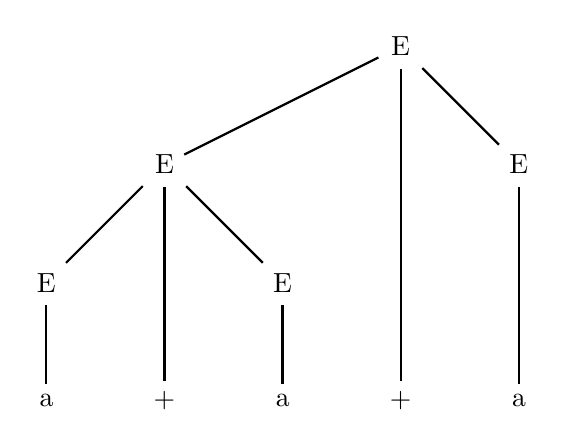
\begin{tikzpicture}[-,>=stealth,shorten >=1pt,auto,node distance=1.5cm,thick,main node/.style={scale=0.9,circle,draw,font=\sffamily\normalsize}]
    
                    \node (1) [] {a};
                    \node (2) [right of=1] {+};
                    \node (3) [right of=2] {a};
                    \node (4) [right of=3] {+};
                    \node (5) [right of=4] {a};
                    
                    \node (6) [above of=1] {E};
                    \node (7) [above of=2] {};
                    \node (8) [above of=3] {E};
                    \node (9) [above of=4] {};
                    \node (10) [above of=5]{};
    
                    \node (11) [above of=6] {};
                    \node (12) [above of=7] {E};
                    \node (13) [above of=8] {};
                    \node (14) [above of=9] {};
                    \node (15) [above of=10]{E};
    
                    \node (16) [above of=11] {};
                    \node (17) [above of=12] {};
                    \node (18) [above of=13] {};
                    \node (19) [above of=14] {E};
                    \node (20) [above of=15] {};
    
                    \path[every node/.style={font=\sffamily\small}]
                    (1) edge (6)
                    (2) edge (12)
                    (3) edge (8)
                    (4) edge (19)
                    (5) edge (15)

                    (6) edge (12)
                    (8) edge (12)

                    (12) edge (19)
                    (15) edge (19)
                    ;
                \end{tikzpicture}
            \end{tabular}

            & \qquad\qquad &

            \begin{tabular}{c}
                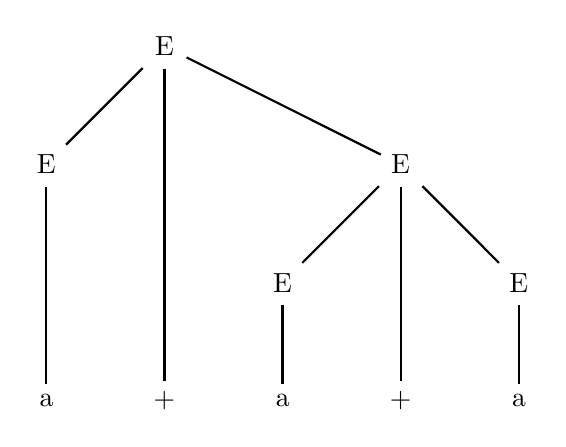
\begin{tikzpicture}[-,>=stealth,shorten >=1pt,auto,node distance=1.5cm,thick,main node/.style={scale=0.9,circle,draw,font=\sffamily\normalsize}]
    
                    \node (1) [] {a};
                    \node (2) [right of=1] {+};
                    \node (3) [right of=2] {a};
                    \node (4) [right of=3] {+};
                    \node (5) [right of=4] {a};
                    
                    \node (6) [above of=1] {};
                    \node (7) [above of=2] {};
                    \node (8) [above of=3] {E};
                    \node (9) [above of=4] {};
                    \node (10) [above of=5] {E};
    
                    \node (11) [above of=6] {E};
                    \node (12) [above of=7] {};
                    \node (13) [above of=8] {};
                    \node (14) [above of=9] {E};
                    \node (15) [above of=10] {};
    
                    \node (16) [above of=11] {};
                    \node (17) [above of=12] {E};
                    \node (18) [above of=13] {};
                    \node (19) [above of=14] {};
                    \node (20) [above of=15] {};
    
                    \path[every node/.style={font=\sffamily\small}]
                    (1) edge (11)
                    (2) edge (17)
                    (3) edge (8)
                    (4) edge (14)
                    (5) edge (10)
                    
                    (8) edge (14)
                    (10) edge (14)
    
                    (11) edge (17)
                    (14) edge (17)
                        ;
                \end{tikzpicture}
            \end{tabular}
        \end{tabular}
    \end{center}

    \begin{frameddefn}{Derivazione a sinistra}
        Data una \CFG $G = (V, \Sigma, R,S)$, definiamo la derivazione $S \derives w$ come \textbf{derivazione sinistra} se ad ogni produzione interna alla derivazione viene valutata la variabile più a sinistra
    \end{frameddefn}

    \textbf{Esempio:}

    \begin{itemize}
        \item Riprendiamo la \CFG dell'esempio precedente:
        \[E \to E+E \smid E \cdot E \smid (E) \smid a\]

        \item Per maggior chiarezza, riscriviamo tali regole come:
        \[E \to E+F \smid E \cdot E \smid (E) \smid a\]
        \[F \to E\]
        ottenendo una \CFG del tutto equivalente alla precedente

        \item Una derivazione sinistra della stringa $a+a+a$ corrisponde a:
        \[E \yields E+F \yields E+F+F \yields a+F+F \yields a+E+F \yields a+a+F \yields a+a+E \yields a+a+a\]
    \end{itemize}

    \begin{framedobs}{}
        L'uso delle derivazioni a sinistra permette di fissare un "ordine", rimuovendo la maggior parte delle derivazioni multiple per una stessa stringa.

        Tuttavia, in alcune grammatiche possono esistere più di una derivazione a sinistra per la stessa stringa.
    \end{framedobs}

    \begin{frameddefn}{Grammatica ambigua}
        Definiamo una grammatica $G$ come \textbf{ambigua} se $\exists w \in L(G)$ tale che esistono almeno due derivazioni a sinistra per $w$
    \end{frameddefn}
    
    \quad
    
    \section{Linguaggi acontestuali ad estensione dei regolari}

    \begin{frameddefn}{Classe dei linguaggi acontestuali}
        Dato un alfabeto $\Sigma$, definiamo come \textbf{classe dei linguaggi acontestuali di $\Sigma$} il seguente insieme:
        \[\CFL = \{L \subseteq \Sigma^* \mid \exists \; \CFG \; G \text{ t.c } L = L(G)\}\]
    \end{frameddefn}

    \begin{framedlem}[label=DFAtoCFG]{Conversione da \DFA a \CFG}
        Date le due classi dei linguaggi $\mathrm{\REG}$ e $\CFL$, si ha che:
        \[\mathrm{\REG} \subseteq \CFL\]
    \end{framedlem}

    \proofenv{
        \begin{itemize}
            \item Dato $L \in \mathrm{\REG}$, sia $D = (Q, \Sigma, \delta, q_0, F)$ il \DFA tale che $L = L(D)$
            \item Consideriamo quindi la \CFG $G = (V, \Sigma, R, S)$ tale che:
            \begin{itemize}
                \item Esiste una funzione biettiva $\funcmap{\varphi}{Q}{V}{q_i}{V_i}$
                \item $S = \varphi(q_0) = V_0$
                \item Dati $q_i,q_j \in Q$ e $a \in \Sigma$, si ha che:
                \[\delta(q_i, a) = q_j \implies \varphi(q_i) \to a \varphi(q_j) \implies V_i \to a V_j\]
                \item $q_f \in F \implies \varphi(q_f) \to \varepsilon \implies V_f \to \varepsilon$
            \end{itemize}

            \item A questo punto, per costruzione stessa di $G$ si ha che:
            \[w \in L(D) \iff w \in L(G)\]
            implicando dunque che $L(D) \in \CFL$ e di conseguenza che:
            \[\mathrm{\REG} \subseteq \CFL\]
        \end{itemize}
    }

    \textbf{Esempio:}

    \begin{itemize}
        \item Consideriamo il seguente \DFA
        
        \begin{center}
            \begin{tikzpicture}[->,>=stealth,shorten >=1pt,auto,node distance=2.5cm,thick,main node/.style={scale=0.9,circle,draw,font=\sffamily\normalsize}]
                \node[initial, state] (1) {$q_1$};
                \node[state] (2) [right of=1] {$q_2$};
                \node[state] (3) [right of=2] {$q_3$};
                \node[state, accepting] (4) [right of=3] {$q_4$};
     
                \path[every node/.style={font=\sffamily\small}]
                    (1) edge [loop above] node {\ttt 0} (1)
                    (2) edge [loop above] node {\ttt 0} (2)
                    (3) edge [loop above] node {\ttt 0} (3)
                    (4) edge [loop above] node {\ttt{0,1}} (4)
                    (1) edge [bend left] node {\ttt 1} (2)
                    (2) edge [bend left] node {\ttt 1} (3)
                    (3) edge [bend left] node {\ttt 1} (4)
                 ;
             \end{tikzpicture}
        \end{center}

        \item Una \CFG $G = (V,\Sigma, R,S)$ equivalente è costituita da:
        \begin{itemize}
            \item $V = \{V_1, V_2, V_3, V_4\}$
            \item $S = V_1$
            \item $R$ definito come:
            \[\begin{array}{l}
                V_1 \to 0V_1 \smid 1 V_2\\
                V_2 \to 0V_2 \smid 1 V_3\\
                V_3 \to 0V_3 \smid 1 V_4\\
                V_4 \to 0V_4 \smid 1 V_4 \smid \varepsilon
            \end{array}\]
        \end{itemize}

        \item Difatti, sia il \DFA sia la \CFG descrivono il seguente linguaggio:
        \[L = \{w \in \Sigma^* \mid \abs{w}_1 \geq 3\}\]
    \end{itemize}

    \newpage

    \begin{framedthm}[label={cfl_reg}]{Ling. acontestuali estensione dei ling. regolari}
        Date le due classi dei linguaggi $\mathrm{\REG}$ e $\CFL$, si ha che:
        \[\mathrm{\REG} \subsetneq \CFL\]
    \end{framedthm}

    \proofenv{
        \begin{itemize}
            \item Tramite la \nameref{DFAtoCFG}, sappiamo che $\mathrm{\REG} \subseteq \CFL$
            \item Consideriamo quindi il linguaggio $L = \{0^n1^n \mid n \in \N\}$
            \item Tale linguaggio è generabile dalla grammatica $G = (\{S\}, \{0,1\}, R, S)$, dove:
            \[S \to 0S1 \smid \varepsilon\]
            dunque abbiamo che $L = L(G) \in \CFL$
            \item Tuttavia, abbiamo già dimostrato nella sezione \ref{non_reg} che $L$ non sia regolare, dunque abbiamo che $L \notin \mathrm{\REG}$
            \item Di conseguenza, concludiamo che:
            \[\mathrm{\REG} \subsetneq \CFL\]
        \end{itemize}
    }

    \quad

    \section{Forma normale di Chomsky}

    \begin{frameddefn}{Chomsky's Normal Form (CNF)}
        Una \CFG $G = (V,\Sigma,R,S)$ viene detta in \textbf{Chomsky's Normal Form (CNF)} (o \textit{Forma Normale di Chomsky}) se tutte le regole in $R$ assumono una delle seguenti tre forme:
        \[A \to BC \qquad\qquad A \to a \qquad\qquad S \to \varepsilon\]
        dove $A \in V$, $a \in \Sigma$ e $B,C \in V-\{S\}$
    \end{frameddefn}

    \begin{framedthm}{Conversione in Forma Normale di Chomsky}
        Per ogni \CFG $G$, si ha che:
        \[\exists \text{ \CFG }\; G' \text{ in CNF } \mid L(G) = L(G')\]
    \end{framedthm}

    \newpage

    \proofenv{
        \begin{itemize}
            \item Data una \CFG $G = (V, \Sigma, R, S)$, costruiamo una \CFG $G'$ in CNF equivalente a $G$:

            \begin{enumerate}
                \item Vengono aggiunte una variabile $S_0$ e una regola $S_0 \to S$, dove $S_0$ è la \textbf{nuova variabile iniziale}
                \item Finché in $R$ esiste una \textbf{$\varepsilon$-regola} $A \to \varepsilon$ dove $A \in V-\{S_0\}$, tale regola viene \textbf{eliminata} e per ogni regola in $R$ contenente delle occorrenze di $A$ vengono \textbf{aggiunte} delle regole in cui vengono eliminate tutte le possibili combinazioni di occorrenze di $A$
                
                (es: se viene rimossa $A \to \varepsilon$ e in $R$ esiste $B \to uAvAw \mid u,v,w \in (V \cup \Sigma)^*$, vengono aggiunte le regole $B \to uvAw \smid uAvw \smid uvw$)
    
                \item Ogni regola nella forma $A \to B$ (dette \textbf{regole unitarie}) viene \textbf{eliminata} e ogni regola nella forma $B \to u$, dove $u \in (V \cup \Sigma)^*$, viene \textbf{sostituita} da una regola $A \to u$ 
                \item Per ogni regola $A \to u_1 \ldots u_k$ dove $k \geq 3$ e $\forall i \in [1,k] \;\; u_i \in (V \cup \Sigma)$, vengono \textbf{aggiunte} le variabili $A_1, \ldots, A_{k-2}$ e le seguenti regole:
                \[A \to u_1A_1 \qquad A_1 \to u_2A_2 \qquad \ldots \qquad A_{k-3} \to u_{k-2}A_{k-2} \qquad A_{k-2} \to u_{k-1}u_k\]
                per poi \textbf{eliminare} la regola iniziale $A \to u_1u_2 \ldots u_k$
                \item Per ogni regola rimanente nella forma $A \to u_1u_2$ dove $u_1,u_2 \in (V \cup \Sigma)$, se $u_1 \in \Sigma$ allora viene \textbf{aggiunta} una variabile $U_1$ ed una regola $U_1 \to u_1$, \textbf{sostituendo} la regola $A \to u_1u_2$ con la regola $A \to U_1u_2$. Analogamente, lo stesso viene svolto se $u_2 \in \Sigma$.
            \end{enumerate}

            \item Poiché le operazioni svolte dall'algoritmo non modificano le stringhe generabili dalla \CFG, ne segue automaticamente che $L(G) = L(G')$
        \end{itemize}
    }


    \textbf{Esempio:}

    \begin{itemize}
        \item Consideriamo la seguente grammatica $G$ non in CNF, dove $S$ è la variabile iniziale:
        \[\begin{array}{llll}
            G:  & S & \to & ASA \smid aB \\
                & A & \to & B \smid S \\
                & B & \to & b \smid \varepsilon
        \end{array}\]

        \item Aggiungiamo la nuova variabile iniziale $S_0$ e la regola $S_0 \to S$:
        \[\begin{array}{llll}
            G:  & \bm{S_0} & \bm{\to} & \bm{S} \\
                & S & \to & ASA \smid aB \\
                & A & \to & B \smid S \\
                & B & \to & b \smid \varepsilon
        \end{array}\]

        \item Eliminiamo la $\varepsilon$-regola $B \to \varepsilon$:
        \[\begin{array}{llll}
            G:  & S_0 & \to & S \\
                & S & \to & ASA \smid aB \smid \bm{a}\\
                & A & \to & B \smid S \smid \bm{\varepsilon}\\
                & B & \to & b \smid \text{\sout{$\varepsilon$}}
        \end{array}\]

        \item Eliminiamo la $\varepsilon$-regola $A \to \varepsilon$:
        \[\begin{array}{llll}
            G:  & S_0 & \to & S \\
                & S & \to & ASA \smid aB \smid a \smid \bm{SA} \smid \bm{AS} \smid \bm{S}\\
                & A & \to & B \smid S \smid \text{\sout{$\varepsilon$}}\\
                & B & \to & b
        \end{array}\]

        \item Eliminiamo la regola unitaria $S \to S$:
        \[\begin{array}{llll}
            G:  & S_0 & \to & S \\
                & S & \to & ASA \smid aB \smid a \smid SA \smid AS \smid \text{\sout{$S$}}\\
                & A & \to & B \smid S\\
                & B & \to & b
        \end{array}\]
        \item Eliminiamo la regola unitaria $S_0 \to S$:
        \[\begin{array}{llll}
            G:  & S_0 & \to & \text{\sout{$S$}} \smid \bm{ASA} \smid \bm{aB} \smid \bm{a} \smid \bm{SA} \smid \bm{AS}\\
                & S & \to & ASA \smid aB \smid a \smid SA \smid AS \\
                & A & \to & B \smid S\\
                & B & \to & b
        \end{array}\]
        \item Eliminiamo le regole unitarie $A \to B$ e $A \to S$:
        \[\begin{array}{llll}
            G:  & S_0 & \to & ASA \smid aB \smid a \smid SA \smid AS\\
                & S & \to & ASA \smid aB \smid a \smid SA \smid AS \\
                & A & \to & \text{\sout{$B$}} \smid \text{\sout{$S$}} \smid \bm{b} \smid \bm{ASA} \smid \bm{aB} \smid \bm{a} \smid \bm{SA} \smid \bm{AS}\\
                & B & \to & b
        \end{array}\]

        \item Separiamo ogni regola con tre o più elementi a destra in regole con massimo due elementi a destra:
        \[\begin{array}{llll}
            G:  & S_0 & \to & \text{\sout{$ASA$}} \smid \bm{AA_1} \smid aB \smid a \smid SA \smid AS\\
                & S & \to & \text{\sout{$ASA$}} \smid \bm{AA_1} \smid aB \smid a \smid SA \smid AS \\
                & A & \to & b \smid \text{\sout{$ASA$}} \smid \bm{AA_1} \smid aB \smid a \smid SA \smid AS\\
                & \bm{A_1} & \bm{\to} & \bm{SA}\\
                & B & \to & b
        \end{array}\]

        \item Infine, convertiamo tutte le regole aventi due elementi a destra di cui almeno uno è un terminale:
        \[\begin{array}{llll}
            G:  & S_0 & \to &  AA_1 \smid \text{\sout{$aB$}} \smid \bm{UB} \smid a \smid SA \smid AS\\
                & S & \to & AA_1 \smid \text{\sout{$aB$}} \smid \bm{UB} \smid a \smid SA \smid AS \\
                & A & \to & b \smid AA_1 \smid \text{\sout{$aB$}} \smid \bm{UB} \smid a \smid SA \smid AS\\
                & A_1 & \to & SA\\
                & \bm{U} & \bm{\to} & \bm{a} \\
                & B & \to & b
        \end{array}\]

        \item La grammatica finale ottenuta risulta sia equivalente a quella iniziale sia in forma normale di Chomsky:
        
        \[\begin{array}{llll}
            G:  & S_0 & \to &  AA_1 \smid UB \smid a \smid SA \smid AS\\
                & S & \to & AA_1 \smid UB \smid a \smid SA \smid AS \\
                & A & \to & b \smid AA_1 \smid UB \smid a \smid SA \smid AS\\
                & A_1 & \to & SA\\
                & U & \to & a \\
                & B & \to & b
        \end{array}\]
    \end{itemize}

    \quad

    \section{Automi a pila}

    \begin{frameddefn}{Pushdown Automaton (\PDA)}
        Un \textbf{Pushdown Automaton (\PDA)} (o \textit{Automa a pila}) è una sestupla $(Q, \Sigma, \Gamma, \delta, q_0, F)$ dove:
        \begin{itemize}
            \item $Q$ è l'\textbf{insieme finito degli stati} dell'automa
            \item $\Sigma$ è l'\textbf{alfabeto} dell'automa
            \item $\Gamma$ è l'\textbf{alfabeto} dello stack (o \textit{pila}) dell'automa
            \item $q_0 \in Q$ è lo \textbf{stato iniziale} dell'automa
            \item $F \subseteq Q$ è l'\textbf{insieme degli stati accettanti} dell'automa 
            \item $\func{\delta}{Q \times \Sigma_{\varepsilon} \times \Gamma_{\varepsilon}}{\mathcal{P}(Q \times \Gamma_{\varepsilon})}$ è la \textbf{funzione di transizione} dell'automa, dove se $(q,c) \in \delta(p,a,b)$ si ha che:
            \begin{itemize}
                \item Viene letto il simbolo $a$ dalla stringa in input e se il simbolo $b$ è in cima allo stack allora l'automa passa dallo stato $p$ allo stato $q$ e il simbolo $b$ viene sostituito dal simbolo $c$
                \item L'etichetta della transizione da $p$ a $q$ viene indicata come $a; \; b \to c$
            \end{itemize}
        \end{itemize}
    \end{frameddefn}

    \begin{framedobs}{}
        Dato $(q,c) \in \delta(p,a,b)$ dove $\delta$ è la funzione di transizione di un \PDA, si ha che:
        \begin{itemize}
            \item Se $b,c = \varepsilon$ (dunque $a; \; \varepsilon \to \varepsilon$) allora l'automa leggerà $a$ dalla stringa e passerà direttamente dallo stato $p$ allo stato $q$, senza modificare lo stack
            \item Se $b = \varepsilon$ e $c \neq \varepsilon$ (dunque $a; \; \varepsilon \to c$) allora l'automa leggerà $a$ dalla stringa, passerà direttamente dallo stato $p$ allo stato $q$ e in cima allo stack viene aggiunto il simbolo $c$ (\textbf{push})
            \item Se $b \neq \varepsilon$ e $c = \varepsilon$ (dunque $a; \; b \to \varepsilon$) allora l'automa leggerà $a$ e se in cima allo stack vi è $b$, l'automa passerà dallo stato $p$ allo stato $q$ e rimuoverà $b$ dalla cima dello stack (\textbf{pop})
        \end{itemize}
    \end{framedobs}

    \textbf{Esempio:}

    \begin{itemize}
        \item Consideriamo il seguente \PDA:
        \begin{center}
            \begin{tikzpicture}[->,>=stealth,shorten >=1pt,auto,node distance=3cm,thick,main node/.style={scale=0.9,circle,draw,font=\sffamily\normalsize}]
    
                \node[initial,state] (1) {$q_1$};
                \node[state, accepting] (2) [right of=1] {$q_2$};
    
                \path[every node/.style={font=\sffamily\small}]
                    (1) edge [loop above] node {\ttt{a; $\varepsilon \to$ c}} (1)
                    (1) edge [] node {\ttt{b; $\varepsilon \to \varepsilon$}} (2)
                    (2) edge [loop above] node {\ttt{$\varepsilon$; $c \to \varepsilon$}} (2)
                    ;
            \end{tikzpicture}
        \end{center}

        \item Data la stringa \ttt{aab}, uno dei possibili rami di computazione del \PDA procede nel seguente ordine:
        \begin{enumerate}
            \item Viene letta la prima \ttt{a} e viene inserita la prima \ttt{c} in cima allo stack, rimanendo nello stato $q_1$.
            \item Viene letta la seconda \ttt{a} e viene inserita la seconda \ttt{c} in cima allo stack, rimanendo nello stato $q_1$.
            \item Viene letta la \ttt{b}, passando da $q_1$ a $q_2$ e lasciando lo stack inalterato
            \item Viene "letta" la prima $\varepsilon$, rimuovendo la seconda \ttt{c} dallo stack (poiché essa è in cima), rimanendo nello stato $q_2$.
            \item Viene "letta" la seconda $\varepsilon$, rimuovendo la prima \ttt{c} dallo stack (poiché essa è in cima), rimanendo nello stato $q_2$.
            \item Sia la stringa che lo stack sono vuoti, dunque la computazione termina necessariamente poiché non vi sono transizioni percorribili
        \end{enumerate}

        \item Notiamo in particolare che, in tal caso, la stringa verrebbe accettata anche se la computazione si fermasse al terzo passo
        \item Difatti, lo stack non deve necessariamente esser vuoto affinché la stringa possa essere accettata 
    \end{itemize}

    \begin{framedprop}{Stringa accettata in un \PDA}
        Sia $P := (Q, \Sigma, \Gamma, \delta, q_0, F)$ un \PDA. Data una stringa $w := w_0 \ldots w_{k} \in \Sigma^*$, dove $w_0, \ldots, w_k \in \Sigma_{\varepsilon}$, diciamo che $w$ è \textbf{accettata da $P$} se esiste una sequenza di stati $r_0, r_1, \ldots, r_{k+1} \in Q$ ed una sequenza di stringhe $s_1, \ldots, s_n \in \Gamma^*$ tali che:
        \begin{itemize}
            \item $r_0 = q_0$
            \item $r_{k+1} \in F$
            \item $s_0 = \varepsilon$, dunque lo stack è inizialmente vuoto
            \item $\forall i \in [0,k]$ si abbia che:
            \begin{itemize}
                \item $(r_{i+1}, b) \in \delta(r_i, w_i, a)$
                \item $s_i = at$
                \item $s_{i+1} = bt$ 
            \end{itemize}
            dove $a,b \in \Gamma_{\varepsilon}$ e dove $t \in \Gamma^*$ è la stringa composta dai caratteri nello stack 
        \end{itemize}
    \end{framedprop}

    \textbf{Esempi:}

    \begin{itemize}
        \item Il seguente automa riconosce il linguaggio $L = \{0^n1^n \mid n \in \N\}$
        
        \quad
        
        \begin{center}
            \begin{tikzpicture}[->,>=stealth,shorten >=1pt,auto,node distance=3cm,thick,main node/.style={scale=0.9,circle,draw,font=\sffamily\normalsize}]
    
                \node[initial,state,accepting] (1) {$q_1$};
                \node[state] (2) [right of=1] {$q_2$};
                \node[state] (3) [below of=2] {$q_3$};
                \node[state,accepting] (4) [left of=3] {$q_4$};
    
                \path[every node/.style={font=\sffamily\small}]
                    (1) edge [] node {\ttt{$\varepsilon$; $\varepsilon \to$ \$}} (2)
                    (2) edge [loop right] node {\ttt{0; $\varepsilon \to$ 0}} (2)
                    (2) edge [] node {\ttt{1; 0 $\to \varepsilon$}} (3)
                    (3) edge [loop right] node {\ttt{1; 0 $\to \varepsilon$ }} (2)
                    (3) edge [] node {\ttt{$\varepsilon$; \$ $\to \varepsilon$}} (4)
                    ;
            \end{tikzpicture}
        \end{center}

        \item Il seguente automa riconosce il linguaggio $L = \{ww^R \mid w \in \{0,1\}^*\}$
        
        \quad
        
        \begin{center}
            \begin{tikzpicture}[->,>=stealth,shorten >=1pt,auto,node distance=3cm,thick,main node/.style={scale=0.9,circle,draw,font=\sffamily\normalsize}]
    
                \node[initial,state,accepting] (1) {$q_1$};
                \node[state] (2) [right of=1] {$q_2$};
                \node[state] (3) [below of=2] {$q_3$};
                \node[state, accepting] (4) [left of=3] {$q_4$};
    
                \path[every node/.style={font=\sffamily\small}]
                    (1) edge [] node {\ttt{$\varepsilon$; $\varepsilon \to$ \$}} (2)
                    (2) edge [loop right] node[align=center]{\ttt{0; $\varepsilon \to$ 0}\\\ttt{1; $\varepsilon \to$ 1}} (2)
                    (2) edge [] node {\ttt{$\varepsilon$;  $\varepsilon \to \varepsilon$}} (3)
                    (3) edge [loop right] node[align=center]{\ttt{0; 0 $\to \varepsilon$}\\\ttt{1; 1 $\to \varepsilon$}} (2)
                    (3) edge [] node {\ttt{$\varepsilon$; \$ $\to \varepsilon$}} (4)
                    ;
            \end{tikzpicture}
        \end{center}
    \end{itemize}

    \quad

    \subsection{Equivalenza tra \CFG e \PDA}

    \begin{frameddefn}{Classe dei linguaggi riconosciuti da un \PDA}
        Dato un alfabeto $\Sigma$, definiamo come \textbf{classe dei linguaggi di $\Sigma$ riconosciuti da un \PDA} il seguente insieme:
        \[\mathcal{L}(\text{\PDA}) = \{L \subseteq \Sigma^* \mid \exists \; \PDA \; P \text{ t.c } L = L(P)\}\]
    \end{frameddefn}

    \begin{framedprop}{Scrittura di una stringa sullo stack}
        Sia $P = (Q, \Sigma, \Gamma, \delta, q_0, F)$ un \PDA. Dati $u_1, \ldots, u_k \in \Gamma$, introduciamo una notazione per cui $\delta$ possa ammettere la scrittura diretta sullo stack della stringa $u := u_1 \ldots u_k$.
        
        Formalmente, diciamo che:
        \[(q, u_1 \ldots u_k) \in \delta(p,a,b) \iff \exists r_1, \ldots, r_{k-1} \in Q \text{ tali che:}\]
        \begin{itemize}
            \item $\delta(p,a,b) \ni (r_1, u_k)$
            \item $\delta(r_1, \varepsilon, \varepsilon) = \{(r_2, u_{k-1})\} $
            \item $\ldots$
            \item $\delta(r_{k-1}, \varepsilon, \varepsilon) = \{(q, u_1)\}$
        \end{itemize}
    \end{framedprop}

    \textbf{Esempio:}

    \begin{itemize}
        \item Dato $(q, xyz) \in \delta(p,a,b)$ si ha che:
        
        \quad

        \begin{center}
            \begin{tikzpicture}[->,>=stealth,shorten >=1pt,auto,node distance=3cm,thick,main node/.style={scale=0.9,circle,draw,font=\sffamily\normalsize}]
    
                \node[state] (1) {$p$};
                \node[state] (2) [right of=1]{$r_1$};
                \node[state] (3) [right of=2]{$r_2$};
                \node[state] (4) [right of=3]{$q$};
    
                \path[every node/.style={font=\sffamily\small}]
                    (1) edge [] node {\ttt{a; b $\to$ z}} (2)
                    (2) edge [] node {\ttt{$\varepsilon$; $\varepsilon \to$ y}} (3)
                    (3) edge [] node {\ttt{$\varepsilon$; $\varepsilon \to$ x}} (4)
                    ;
            \end{tikzpicture}
        \end{center}
    \end{itemize}

    \begin{framedlem}[label=cfg_to_pda]{Conversione da \CFG a \PDA}
        Date le due classi dei linguaggi $\CFL$ e $\mathcal{L}(\PDA)$, si ha che:
        \[\CFL \subseteq \mathcal{L}(\PDA)\]
    \end{framedlem}

    \proofenv{
        \begin{itemize}
            \item Dato $L \in \CFL$, sia $G = (V, \Sigma, R,S)$ la \CFG tale che $L = L(G)$
            \item Consideriamo quindi il \PDA $P = (Q, \Sigma, \Gamma, \delta, q_{\mathrm{start}}, F)$ tale che:
            
            \begin{itemize}
                \item $Q = \{q_{\mathrm{start}}, q_{\mathrm{loop}}, q_{\mathrm{accept}}\} \cup Q_{\delta}$, dove $Q_{\delta}$ sono i minimi stati aggiunti affinché la sua funzione $\delta$ sia ben definita (vedi i punti successivi)
                \item $\Gamma = V \cup \Sigma$
                \item $F = \{q_{\mathrm{accept}}\}$
                \item Dato $q_{\mathrm{start}} \in Q$ si ha che
                \[\delta(q_{\mathrm{start}}, \varepsilon, \varepsilon) = \{(q_{\mathrm{loop}}, S\$)\}\]
                \item $\forall A \in V$ si ha che
                \[\delta(q_{\mathrm{loop}}, \varepsilon, A) = \{(q_{\mathrm{loop}}, u) \mid (A \to u) \in R, \; u \in \Gamma^*\}\]
                \item $\forall a \in \Sigma$ si ha che
                \[\delta(q_{\mathrm{loop}}, a, a) = \{(q_{\mathrm{loop}}, \varepsilon)\}\]
                \item Dato $q_{\mathrm{accept}} \in Q$ si ha che
                \[\delta(q_{\mathrm{loop}}, \varepsilon, \$) = \{(q_{\mathrm{accept}}, \varepsilon)\}\]
            \end{itemize}

            \item A questo punto, per costruzione stessa di $P$ si ha che:
            \[w \in L = L(G) \iff w \in L(P)\]
            dunque che $L = L(P) \in \mathcal{L}(\text{\PDA})$
        \end{itemize}
    }

    \textbf{Esempio:}

    \begin{itemize}
        \item Consideriamo la seguente grammatica:
        \[\begin{array}{ll}
            G:  & S \to aTb \smid b\\
                & T \to Ta \smid \varepsilon
        \end{array}\]

        \item Il \PDA in grado di riconoscere $L(G)$ corrisponde a:
    \end{itemize}

    \begin{center}
        \begin{tikzpicture}[->,>=stealth,shorten >=1pt,auto,node distance=3.5cm,thick,main node/.style={scale=0.9,circle,draw,font=\sffamily\normalsize}]

            \node[initial, state] (1) {$q_{\mathrm{start}}$};
            \node[state] (2) [right of=1]{$r_1$};
            \node[state] (3) [right of=2]{$q_{\mathrm{loop}}$};
            \node[state, accepting] (4) [right of=3]{$q_{\mathrm{accept}}$};

            \node[state] (5) [below of=1]{$r_2$};
            \node[state] (6) [below of=2]{$r_3$};
            \node[state] (7) [below of=4]{$r_4$};

            \path[every node/.style={font=\sffamily\small}]
                (1) edge [] node {\ttt{$\varepsilon$; $\varepsilon \to$ \$}} (2)
                (2) edge [] node {\ttt{$\varepsilon$; $\varepsilon \to$ S}} (3)
                (3) edge [] node {\ttt{$\varepsilon$; \$ $\to \varepsilon$}} (4)

                (3) edge [loop above] node[align=center]{
                    \ttt{$\varepsilon$; S $\to$ b}\\
                    \ttt{$\varepsilon$; T $\to \varepsilon$}\\
                    \ttt{a; a $\to \varepsilon$}\\
                    \ttt{b; b $\to \varepsilon$}
                } (3)

                (3) edge [left] node {\ttt{$\varepsilon$; S $\to$ b $\;$}} (5)
                (5) edge [below] node {\ttt{$\varepsilon$; $\varepsilon \to$ T}} (6)
                (6) edge [right] node[near start]{\ttt{ $\varepsilon$; $\varepsilon \to$ a}} (3)

                (3) edge [bend left] node[near end]{\ttt{$\varepsilon$; T $\to$ a}} (7)
                (7) edge [bend left] node[near start]{\ttt{$\varepsilon$; $\varepsilon \to$ T}} (3)

                ;
        \end{tikzpicture}
    \end{center}


    \begin{framedlem}{Conversione da \PDA a \CFG}
        Date le due classi dei linguaggi $\mathcal{L}(\PDA)$ e $\CFL$, si ha che:
        \[\mathcal{L}(\PDA) \subseteq \CFL\]
    \end{framedlem}

    \proofenv{
        \begin{itemize}
            \item Dato $L \in \mathcal{L}(\PDA)$, sia $P = (Q, \Sigma, \Gamma, \delta, q_0, F)$ il \PDA tale che $L = L(P)$
            \item Consideriamo il \PDA $P' = (Q', \Sigma, \Gamma, \delta', q_0, \{q_{\mathrm{accept}}\})$ tale che:
            \begin{itemize}
                \item Ogni transizione effettua solo un'operazione di push o di pop, ma mai una sostituzione diretta:
                \[(q,c) \in \delta(p,a,b) \implies \exists r \in Q' \mid (r, \varepsilon) \in \delta'(p,a,b) \land \delta'(r, \varepsilon, \varepsilon) = \{(q,c)\}\]
                \item $Q' = Q \cup Q_{\delta'} \cup \{q_{\mathrm{accept}}\}$, dove $Q_{\delta'}$ sono gli stati aggiunti per il punto precedente
                \item $q_{\mathrm{accept}} \in Q'$ è il nuovo unico stato accettante:
                \[\forall q \in F \;\; (q_{\mathrm{accept}}, \varepsilon) \in \delta'(q, \varepsilon, \varepsilon)\]
                \item Lo stack deve essere svuotato prima di poter accettare una stringa:
                \[\forall q \in F, a \in \Sigma \;\; (q, \varepsilon) \in \delta'(q, \varepsilon, a)\]
            \end{itemize}

            \item A questo punto, per costruzione stessa di $P'$ si ha che:
            \[w \in L(P) \iff w \in L(P')\]
            dunque che $L = L(P) = L(P')$

            \item Consideriamo quindi la \CFG $G = (V, \Sigma, R, S)$ tale che:
            \begin{itemize}
                \item $V = \{A_{p,q} \mid p,q \in Q'\}$
                \item $S = A_{q_0, q_{\mathrm{accept}}}$
                \item Ogni variabile $A_{p,q}$ è grado di derivare tutte le stringhe generabili passando dallo stato $p$ allo stato $q$:
                \begin{itemize}
                    \item $\forall p \in Q'$ si ha che:
                    \[(A_{p,p} \to \varepsilon) \in R\]
                    \item $\forall p,q,r,s \in Q', u \in \Gamma$ e $a,b \in \Sigma_{\varepsilon}$ si ha che:
                    \[(r, u) \in \delta'(p,a,\varepsilon) \land (q,\varepsilon) \in \delta(s,b,u) \iff (A_{p,q} \to aA_{r,s}b) \in R\]
                    \item $\forall p,q,r \in Q'$ si ha che:
                    \[(A_{p,q} \to A_{p,r}A_{r,q}) \in R\]
                \end{itemize}
            \end{itemize}

            \item \textbf{Affermazione}: dati $p,q \in Q'$ e $x \in \Sigma^*$, se $A_{p,q} \derives x$ allora $x$ porta il \PDA $P'$ dallo stato $p$ allo stato $q$ con uno stack vuoto:
            
            \textit{Dimostrazione.}

            Procediamo per induzione sul numero $n$ di produzioni che compongono la derivazione $A_{p,q} \derives x$

            \begin{enumerate}[label=]
                \item \textit{Caso base.}
                
                \begin{itemize}
                    \item Per $n=1$, la derivazione è composta da una sola produzione. Di conseguenza, l'unica regola possibile affinché $A_{p,q} \yields x$ è la regola $A_{p,q} \to \varepsilon$, implicando che $p = q$ e che $x = \varepsilon$, dunque la stringa $x$ porta correttamente il \PDA $P'$ dallo stato $p$ allo stato $q$ con uno stack vuoto 
                \end{itemize}

                \item \textit{Ipotesi induttiva forte.}
                
                \begin{itemize}
                    \item Assumiamo che per ogni stringa $x \in \Sigma^*$ derivabile da $A_{p,q}$ (dunque tale che $A_{p,q} \derives x$) tramite $k \leq n$ produzioni, tale stringa $x$ porti il \PDA $P'$ da $p$ a $q$ con uno stack vuoto
                \end{itemize}

                \item \textit{Passo induttivo.}
                
                \begin{itemize}
                    \item Consideriamo la derivazione $A_{p,q} \derives x$ composta da $n+1$ produzioni. Poiché tale derivazione è composta da almeno due produzioni, la prima produzione deve essere necessariamente data dalla regola $A_{p,q} \to aA_{r,s}b$ o dalla regola $A_{p,q} \to A_{p,r}A_{r,q}$
                    
                    \begin{enumerate}
                        \item Consideriamo il caso in cui $A_{p,q} \yields aA_{r,s}b \derives x$.
                        
                        Sia $x = ayb$, dove $A_{r,s} \derives y$. Poiché $A_{r,s} \derives y$ è composta da $n$ produzioni, per ipotesi induttiva la stringa $y$ porta il \PDA $P'$ da $r$ ad $s$ con uno stack vuoto.

                        Inoltre, per costruzione stessa di $G$, tale regola di derivazione si ha che:
                        \[(r, u) \in \delta'(p,a,\varepsilon) \land (q,\varepsilon) \in \delta(s,b,u) \iff (A_{p,q} \to aA_{r,s}b) \in R\]
                        dunque concludiamo che:
                        \[\left . \begin{array}{l}
                            a \text{ porta } P' \text{ da } p \text{ in } r\\
                            y \text{ porta } P' \text{ da } r \text{ in } s\\
                            b \text{ porta } P' \text{ da } s \text{ in } q\\
                        \end{array} \right \} \implies x = ayb \text{ porta } P' \text{ da } p \text{ in } q\]

                        \item Consideriamo il caso in cui $A_{p,q} \yields A_{p,r}A_{r,q}\derives x$.
                        
                        Sia $x = yz$, dove $A_{p,r} \derives y$ e $A_{r,q} \derives z$. Poiché $A_{p,r} \derives y$ è composta da $m \leq n$ produzioni e $A_{r,q} \derives z$ da $n-m \leq n$ produzioni, per ipotesi induttiva le stringhe $y$ e $z$ portano il \PDA $P'$ rispettivamente da $p$ ad $r$ e da $r$ a $q$ con uno stack vuoto, dunque concludiamo che:
                        \[\left . \begin{array}{l}
                            y \text{ porta } P' \text{ da } p \text{ in } r\\
                            z \text{ porta } P' \text{ da } r \text{ in } q\\
                        \end{array} \right \} \implies x = yz \text{ porta } P' \text{ da } p \text{ in } q\]
                    \end{enumerate}
                \end{itemize}
            \end{enumerate}

            \item \textbf{Affermazione}: dati $p,q \in Q'$ e $x \in \Sigma^*$, se la stringa $x$ porta il \PDA $P'$ dallo stato $p$ allo stato $q$ con uno stack vuoto allora $A_{p,q} \derives x$
            
            \textit{Dimostrazione.}

            Procediamo per induzione sul numero $n$ di transizioni percorse da $P'$ durante la lettura di $x$

            \begin{enumerate}[label=]
                \item \textit{Caso base.}
                
                \begin{itemize}
                    \item Per $n=0$, il \PDA percorre zero transizioni, dunque $x = \varepsilon$ e $x$ porta il \PDA da $p$ a $p$. Pertanto, la regola $A_{p,p} \to \varepsilon$ soddisfa la derivazione $A_{p,p} \yields x$
                \end{itemize}

                \item \textit{Ipotesi induttiva forte.}
                
                \begin{itemize}
                    \item Assumiamo che per ogni stringa $x \in \Sigma^*$ che porta il \PDA $P'$ da $p$ a $q$ con uno stack vuoto percorrendo $k \leq n$ transizioni, si abbia che $A_{p,q} \derives x$
                \end{itemize}

                \item \textit{Passo induttivo.}
                
                \begin{itemize}
                    \item Consideriamo la stringa $x \in \Sigma^*$ che porta il \PDA $P'$ da $p$ a $q$ con uno stack vuoto percorrendo $n+1$ transizioni. A seconda dell'evolvere dello stack durante la computazione, abbiamo due casi:
                    \begin{enumerate}
                        \item Se lo stack risulta vuoto solo all'inizio e alla fine della computazione, ciò implica che $\exists u \in \Gamma$ inserito nella prima transizione e rimosso solo nell'ultima.
                        
                        Sia quindi $a \in \Sigma_{\varepsilon}$ il simbolo letto durante tale prima transizione. In tal caso, $\exists r,s \in Q'$ tali che:
                        \[(r,u) \in \delta(p,a,\varepsilon) \land (q,\varepsilon) \in \delta(s,b,u)\]

                        Sia quindi $x = ayb$, dove $y$ è una stringa che porta $P'$ da $r$ a $s$. Affinché la computazione di $x$ termini con lo stack vuoto, è necessario che ciò valga anche per la computazione di $y$.
                        
                        Poiché la computazione di $y$ percorre $n-1$ transizioni, per ipotesi induttiva abbiamo che $A_{r,s} \derives y$, dunque data la regola $A_{p,q} \to aA_{r,s}b$ concludiamo che:
                        \[A_{p,q} \yields aA_{r,s}b \derives ayb = x\]

                        \item Se lo stack si svuota durante la computazione, ciò implica che $\exists r \in Q'$ percorso durante la computazione di $x$ in cui ciò accade.
                        
                        Sia quindi $x = yz$, dove $y$ e $z$ sono due stringhe che portano $P'$ rispettivamente da $p$ a $r$ e da $r$ a $q$.
                        
                        Poiché le computazioni di $y$ e $z$ percorrono rispettivamente $m \leq n$ e $n-m \leq n$ transizioni, per ipotesi induttiva abbiamo che $A_{p,r} \derives y$ e $A_{r,q} \derives z$, dunque data la regola $A_{p,q} \to A_{p,r}A_{r,q}$ concludiamo che:
                        \[A_{p,q} \yields A_{p,r}A_{r,q} \derives yz = x\]
                    \end{enumerate}
                \end{itemize}
                
            \end{enumerate}
            
            \item Tramite le due affermazioni, abbiamo che:
            \[A_{q_0, q_{\mathrm{accept}}} \derives x \iff x \text{ porta } P' \text{ da } q_0 \text{ in } q_{\mathrm{accept}} \text{ con uno stack vuoto}\]
            da cui concludiamo che:
            \[x \in L(G) \iff A_{q_0, q_{\mathrm{accept}}} \derives x \iff x \in L(P')\]
            dunque che $L = L(P) = L(P') = L(G) \in \CFL$
        \end{itemize}
    }

    \begin{framedthm}{Equivalenza tra \CFG e \PDA}
        Date le due classi dei linguaggi $\mathcal{L}(\PDA)$ e $\CFL$, si ha che:
        \[\mathcal{L}(\PDA) = \CFL\]

        (\textit{segue dai due lemmi precedenti})
    \end{framedthm}
    
    \quad

    \section{Pumping lemma per i linguaggi acontestuali}

    \begin{framedprop}{Altezza delle derivazioni in una \CFG in CNF}
        Sia $G = (V, \Sigma, R,S)$ una \CFG in CNF. Data $x \in L(G)$ e data l'altezza $h$ dell'albero di derivazione di $x$, si ha che $\abs{x} \leq 2^{h-1}$
    \end{framedprop}

    \proofstrind{
        Procediamo per induzione sul'altezza $h$ dell'albero di $S \derives x$
    }{
        \begin{itemize}
            \item Per $h = 1$, la derivazione è composta da una sola produzione. Essendo $G$ in CNF, l'unica regola applicabile è nella forma $S \to a$, dove $x = a \in \Sigma$, implicando che $\abs{x} = 1 \leq 2^{1-1} = 1$
        \end{itemize}
    }{
        \begin{itemize}
            \item Assumiamo che data $x \in L(G)$ tale che il suo albero di derivazione abbia altezza $k \leq h$ si abbia che $\abs{x} \leq 2^{h-1}$
        \end{itemize}
    }{
        \begin{itemize}
            \item Consideriamo la stringa $x$ il cui albero di derivazione ha altezza $h+1$. Poiché $G$ è in CNF, la prima produzione di tale derivazione deve essere ottenuta tramite una regola nella forma $S \to AB$.
            \item Sia quindi $x = yz$, dove $A \derives y$ e $B \derives z$. Poiché la derivazione $S \yields AB \derives yz = x$ ha altezza $h+1$, ne segue che l'altezza dei due sottoalberi delle derivazioni $A \derives y$ e $B \derives z$ sia $h$
            \item Di conseguenza, per ipotesi induttiva si ha che $\abs{y} \leq 2^{h-1}$ e $\abs{z} \leq 2^{h-1}$, implicando che:
            \[\abs{x} = \abs{y}+ \abs{z} \leq 2^{h-1} + 2^{h-1} = 2^{h} = 2^{(h+1)-1}\]
        \end{itemize}
    }

    \begin{framedlem}[label=pumpCFL]{Pumping lemma per i linguaggi acontestuali}
        Dato un linguaggio $L$, se $L \in \CFL$ allora $\exists p \in \N$, detto \textbf{lunghezza del pumping}, tale che $\forall w := uvxyz \in L$, con $\abs{w} \geq p$ e $u,v,x,y,z \in \Sigma^*$ (ossia sono sue sottostringhe), si ha che:
        \begin{itemize}
            \item $\forall i \in \N \;\; uv^ixy^iz \in L$
            \item $\abs{vy} > 0$, dunque $v \neq \varepsilon$ o $y \neq \varepsilon$
            \item $\abs{vxy} \leq p$
        \end{itemize}
    \end{framedlem}

    \proofenv{
        \begin{itemize}
            \item Dato $L \in \CFL$, sia $G = (V, \Sigma, R,S)$ la \CFG in CNF tale che $L = L(G)$
            \item Sia $p = 2^{\abs{V}}$. Data una stringa $w \in L$ tale che $\abs{w} \geq p$, per la proposizione precedente l'albero di derivazione di $w$ deve avere un'altezza $h \geq \abs{V}+1$, poiché altrimenti $w$ non sarebbe generabile da esso
            \item Consideriamo quindi un cammino di lunghezza $h$ di tale albero, dunque passante per almeno $k \geq \abs{V}+2$ nodi. Trattandosi di un cammino all'interno di un albero di derivazione, solo l'ultimo nodo del cammino corrisponderà ad un terminale, implicando che in tale cammino vi siano $k-1 \geq \abs{V}+1$ variabili.
            \item Sia quindi $A_1, \ldots, A_{k-1}$ la sequenza di variabili del cammino (dove $S = A_1$). Poiché  $k-1 \geq \abs{V}+1 \geq \abs{V}$, ne segue necessariamente che $\exists i, j \mid k-\abs{V}-2 \leq i < j \leq k-1 \land A_i = A_j$, ossia che tra le ultime $\abs{V}+1$ variabili del cammino vi sia almeno una variabile ripetuta
            \item Consideriamo quindi le cinque sottostringhe $u,v,x,y,z \in \Sigma^*$ tali che:
            \begin{itemize}
                \item $w = uvxyz$
                \item $S \derives u A_i z$
                \item $A_i \derives vA_jy$
                \item $A_j \derives x$
            \end{itemize}

            \newpage

            \item Poiché $A_i = A_j$, all'interno di ogni derivazione $A_i \derives vA_jy$ possiamo sostituire $A_j$ con $A_i$ stesso. Ripetendo tale procedimento $i \in \N$ volte ricorsivamente, otteniamo che:
            \[A_i \derives vA_jy = vA_iy \derives v^i A_j y^i \yields v^ixy^i\]
            implicando dunque che $\forall i \in \N \;\; S \derives uv^ixy^iz$ e quindi che $uv^ixy^iz \in L(G) = L$
            \item Poiché $G$ è in CNF, dunque al suo interno non possono esserci $\varepsilon$-regole o regole unitarie, la derivazione $A_i \derives vA_jy$ deve necessariamente aver utilizzato una regola del tipo $A_i \to BC$ dove $B \derives vA_j$ e $C \derives y$ oppure $B \derives v$ e $C \derives A_jy$. Poiché non vi sono $\varepsilon$-regole, in entrambi i casi si ha che $v \neq \varepsilon$ o $y \neq \varepsilon$, implicando che $\abs{vy} > 0$
            \item Poiché $A_i$ si trova tra le ultime $\abs{V}+1$ variabili del cammino, ne segue che il suo sottoalbero abbia altezza $h' \leq \abs{V}+1$ (contando anche il terminale finale). Per la proposizione precedente, dunque, ne segue che:
            \[\abs{vxy} \leq 2^{h'-1} \leq 2^{\abs{V}} = p\]
        \end{itemize}
    }

    \begin{center}
        \includegraphics[scale=0.55]{images/pumpCFL.png}

        \textit{Rappresentazione grafica della dimostrazione}
    \end{center}

    \newpage

    \textbf{Esempio:}

    \label{non_cfl}

    \begin{enumerate}
        \item \begin{itemize}
            \item Consideriamo il linguaggio $L = \{0^n1^n2^n \mid n \in \N\}$
            \item Supponiamo per assurdo che $L \in \CFL$. In tal caso, ne segue che per esso debbia valere il pumping lemma, dove $p$ è la lunghezza del pumping
            \item Consideriamo quindi la stringa $w := 0^p1^p2^p$. Poiché $\abs{w} \geq p$, possiamo suddividerla in cinque sottostringhe $u,v,x,y,z \in \Sigma^*$ tali che $w = uvxyz$.
            \item Poiché la terza condizione del pumping lemma impone che $\abs{vxy} \leq p$, le uniche possibilità sono:
            \begin{enumerate}
                \item Se $vxy = 0^m$ con $1 \leq m \leq p$, si ha che $u = 0^h$ e $z = 0^{p-m-h}1^p2^p$, dove $1 \leq m+h \leq p$. Inoltre, poiché la seconda condizione impone che $\abs{vy} > 0$, si ha che $v$ e/o $y$ contengono almeno uno 0
                
                \item Se $vxy = 1^m$ con $1 \leq m \leq p$, si ha che $u = 0^p1^h$ e $z = 1^{p-m-h}2^p$, dove $1 \leq m+h \leq p$. Inoltre, poiché la seconda condizione impone che $\abs{vy} > 0$, si ha che $v$ e/o $y$ contengono almeno un 1
                
                \item Se $vxy = 2^m$ con $1 \leq m \leq p$, si ha che $u = 0^p1^p$ e $z = 2^{p-m-h}$, dove $\ leq m+h \leq p$. Inoltre, poiché la seconda condizione impone che $\abs{vy} > 0$, si ha che $v$ e/o $y$ contengono almeno un 2
                
                \item Se $vxy = 0^m1^h$ con $1 \leq m+h \leq p$, si ha che $u = 0^{p-m}$ e $z = 1^{p-h}2^{p}$. Inoltre, poiché la seconda condizione impone che $\abs{vy} > 0$, si ha che $v$ contiene almeno uno 0 e/o $y$ contiene almeno un 1 
                
                \item Se $vxy = 1^m2^h$ con $1 \leq m+h \leq p$, si ha che $u = 0^{p}1^{p-m}$ e $z = 2^{p-h}$. Inoltre, poiché la seconda condizione impone che $\abs{vy} > 0$, si ha che $v$ contiene almeno uno 1 e/o $y$ contiene almeno un 2
            \end{enumerate}
    
            \item In tutti i casi possibili descritti, risulta automatico che
            \[\nexists n \in \N \mid n = \abs{uv^0xy^0z}_0 = \abs{uv^0xy^0z}_1 = \abs{uv^0xy^0z}_2 \implies uv^0xy^0z \notin L\]
            contraddicendo quindi la prima condizione del pumping lemma
            \item Di conseguenza, ne segue necessariamente che $L \notin \CFL$
        \end{itemize}

        \quad
        \item \begin{itemize}
            \item Consideriamo il linguaggio $L = \{ww \mid w \in \{0,1\}^*\}$
            \item Supponiamo per assurdo che $L \in \CFL$. In tal caso, ne segue che per esso debbia valere il pumping lemma, dove $p$ è la lunghezza del pumping
            \item Consideriamo quindi la stringa $w := 0^p1^p0^p1^p$. Poiché $\abs{w} \geq p$, possiamo suddividerla in cinque sottostringhe $u,v,x,y,z \in \Sigma^*$ tali che $w = uvxyz$.

            \newpage

            \item Poiché la terza condizione del pumping lemma impone che $\abs{vxy} \leq p$, le uniche possibilità sono:
            \begin{enumerate}
                \item Se $u = 0^h$, $vxy = 0^m$ e $z = 0^{p-m-h}1^p0^p1^p$, dove $1 \leq m+h \leq p$, poiché la seconda condizione impone che $\abs{vy} > 0$, si ha che $v$ e/o $y$ contengono almeno uno 0, dunque si ha che:
                \[\exists k < m \mid v^0xy^0 = 0^k \implies uv^0xy^0z = 0^h0^k0^{p-m-h}1^p0^p1^p = 0^{p-m+k}1^p0^p1^p\]
                dove $k < m \implies p-m-k < p$ e dunque che $uv^0xy^0z \notin L$

                \item Se $u = 0^p1^p0^h$, $vxy = 0^m$ e $z = 0^{p-m-h}1^p$, dove $1 \leq m+h \leq p$, procedendo analogamente al caso $(a)$ otteniamo che $uv^0xy^0z \notin L$

                \item Se $u = 0^p1^h$, $vxy = 1^m$ e $z = 1^{p-m-h}0^p1^p$, dove $1 \leq m+h \leq p$, procedendo analogamente al caso $(a)$ otteniamo che $uv^0xy^0z \notin L$

                \item Se $u = 0^p1^p0^p1^h$, $vxy = 1^m$ e $z = 1^{p-m-h}$, dove $1 \leq m+h \leq p$, procedendo analogamente al caso $(a)$ otteniamo che $uv^0xy^0z \notin L$

                \item Se $u = 0^{p-h}$, $vxy = 0^h1^m$ e $z = 1^{p-m}0^p1^p$, dove $1 \leq m+h \leq p$, poiché la seconda condizione impone che $\abs{vy} > 0$, si ha che $v$ contiene almeno uno 0 e/o $y$ contiene almeno un 1, dunque si ha che:
                \[\exists j < h, j < m \mid v^0xy^0 = 0^j1^k \implies\]
                \[uv^0xy^0z = 0^{p-h}0^j1^k1^{p-m}0^p1^p = 0^{p-h+j}1^{p-m+k}0^p1^p\]
                dove $j < h, k < m \implies p-h+j, p-m+k < p$ e dunque che $uv^0xy^0z \notin L$ 

                \item Se $u = 0^p1^p0^{p-h}$, $vxy = 0^h1^m$ e $z = 1^{p-m}$, dove $1 \leq m+h \leq p$, procedendo analogamente al caso $(e)$ otteniamo che $uv^0xy^0z \notin L$

                \item Se $u = 0^p1^{p-h}$, $vxy = 1^h0^m$ e $z = 0^{p-m}1^p$, dove $1 \leq m+h \leq p$, poiché la seconda condizione impone che $\abs{vy} > 0$, si ha che $v$ contiene almeno uno 1 e/o $y$ contiene almeno un 0, dunque si ha che:
                \[\exists j < h, j < m \mid v^0xy^0 = 1^j0^k \implies\]
                \[uv^0xy^0z = 0^p1^{p-h}1^j0^k0^{p-m}1^p = 0^p1^{p-h+j}0^{p-m+k}1^p\]
                dove $j < h, k < m \implies p-h+j, p-m+k < p$ e dunque che $uv^0xy^0z \notin L$ 
            \end{enumerate}

            \item Di conseguenza, poiché il pump down non può essere effettuato nè in un blocco di soli 0 o soli 1 (casi $a, b, c, d$), nè a cavallo tra degli 0 ed 1 (casi $e,f$), nè al centro della stringa (caso $g$), ne segue che la prima condizione del pumping lemma venga contraddetta
            \item Di conseguenza, ne segue necessariamente che $L \notin \CFL$
        \end{itemize}
    \end{enumerate}
    
    \newpage

    \section{Chiusure dei linguaggi acontestuali}

    \begin{framedthm}{Chiusura dell'unione in $\CFL$}
        L'operatore unione è \textbf{chiuso in $\CFL$}, ossia:
        \[\forall L_1, \ldots, L_n \in \CFL \;\; L_1 \cup \ldots \cup L_n \in \CFL\]
    \end{framedthm}

    \proofenv{
        \begin{itemize}
            \item Dati $L_1, \ldots, L_n \in \CFL$, siano $G_1, \ldots, G_n$ le grammatiche tali che $\forall i \in [1,n] \; G_i = (V_i, \Sigma_i, R_i, S_i)$, dove $L_i = L(G_i)$ e $\forall i \neq j$ si ha che $V_i \cap V_j = \varepsilon$.
    
            \item Consideriamo quindi la \CFG $G = (V, \Sigma, R, S)$ tale che:
            \begin{itemize}
                \item $S$ è una nuova variabile iniziale
                \item $V = \rbk{\bigcup\limits_{i = 0}^n V_i} \cup \{S\}$
                \item $\Sigma = \bigcup\limits_{i = 0}^n \Sigma_i$
                \item $R = \rbk{\bigcup\limits_{i = 0}^n R_i} \cup \{ S \to S_j \mid j \in [1,n]\}$
            \end{itemize}

            \item Data $w \in \bigcup\limits_{i = 0}^n L(G_i)$, si ha che $\exists j \in [1,n] \mid w \in L(G_j)$
            
            Di conseguenza, poiché $(S \to S_j) \in R$, ne segue che 
            \[w \in L(G_j) \iff S_j \derives w \implies S \yields S_j \derives w \implies w \in L(G)\]

            \item Data $w \in L(G)$, invece, dove $w \in L(G) \iff S \derives w$, poiché le uniche regole applicabili su $S$ sono $\{ S \to S_j \mid j \in [1,n]\}$, ne segue necessariamente che:
            \[w \in L(G) \implies \exists j \in [0,n] \mid S \yields S_j \derives w \implies w \in L(G_j) \subseteq \bigcup_{i = 0}^n L(G_i)\]

            \item Di conseguenza, concludiamo che:
            \[L_1 \cup \ldots \cup L_n = L(G_1) \cup \ldots \cup L(G_n) = L(G) \in \CFL\]
        \end{itemize}
    }

    \newpage

    \begin{framedthm}{Chiusura della concatenazione in $\CFL$}
        L'operatore concatenazione è \textbf{chiuso in $\CFL$}, ossia:
        \[\forall L_1, \ldots, L_n \in \CFL \;\; L_1 \circ \ldots \circ L_n \in \CFL\]
    \end{framedthm}

    \proofenv{
        \begin{itemize}
            \item Dati $L_1, \ldots, L_n \in \CFL$, siano $G_1, \ldots, G_n$ le grammatiche tali che $\forall i \in [1,n] \; G_i = (V_i, \Sigma_i, R_i, S_i)$, dove $L_i = L(G_i)$ e $\forall i \neq j$ si ha che $V_i \cap V_j = \varepsilon$.
    
            \item Consideriamo quindi la \CFG $G = (V, \Sigma, R, S)$ tale che:
            \begin{itemize}
                \item $S$ è una nuova variabile iniziale
                \item $V = \rbk{\bigcup\limits_{i = 0}^n V_i} \cup \{S\}$
                \item $\Sigma = \bigcup\limits_{i = 0}^n \Sigma_i$
                \item $R = \rbk{\bigcup\limits_{i = 0}^n R_i} \cup \{ S \to S_1\ldots S_n\}$
            \end{itemize}

            \item Sia $w := w_1\ldots w_n \in L(G_1) \circ \ldots \circ L(G_n)$, dove $\forall j \in [1,n] \;\; w_j \in L(G_j)$
            
            Poiché $(S \to S_1 \ldots S_n) \in R$, ne segue che 
            \[\forall j \in [1,n]\;\; w_i \in L(G_j) \iff S_j \derives w_j\]
            dunque abbiamo che:
            \[S \yields S_1 \ldots S_n \derives w_1 \ldots w_n = w \implies w \in L(G)\]

            \item Data $w \in L(G)$, invece, dove $w \in L(G) \iff S \derives w$, poiché l'unica regola applicabile su $S$ è $S \to S_1 \ldots S_n$, ne segue necessariamente che:
            \[w \in L(G) \implies S \yields S_1 \ldots S_n \derives w\]
            dunque $\exists w_1 \in L(G_1), \ldots, w_n \in L(G_n)$ tali che:
            \[S \yields S_1 \ldots S_n \derives w_1 S_2 \ldots S_n \derives w_1 w_2 \ldots w_n = w\]
            implicando che:
            \[w = w_1 w_2 \ldots w_n \in L(G_1) \circ \ldots \circ L(G_n)\]

            \item Di conseguenza, concludiamo che:
            \[L_1 \circ \ldots \circ L_n = L(G_1) \circ \ldots \circ L(G_n) = L(G) \in \CFL\]
        \end{itemize}
    }

    \newpage

    \textbf{Esempio:}

    \begin{itemize}
        \item Consideriamo i seguenti linguaggi:
        \[L_1 = \{0^n1^n \mid n \in \N\} \qquad L_2 = \{1^m0^m \mid m \in \N\}\]
        \item Consideriamo quindi le due grammatiche:
        \[G_1 : A \to 0A1 \smid \varepsilon\]
        \[G_2 : B \to 1A0 \smid \varepsilon\]
        tali che $L_1 = L(G_1)$ e $L_2 = L(G_2)$
        \item La grammatica $G$ tale che $L(G) = L_1 \cup L_2$, corrisponderà a:
        \[\begin{array}{ll}
            G:  & S \to A \smid B \\
                & A \to 0A1 \smid \varepsilon\\
                & B \to 0B1 \smid \varepsilon
        \end{array}\]
        \item La grammatica $G'$ tale che $L(G') = L_1 \circ L_2$, corrisponderà a:
        \[\begin{array}{ll}
            G:  & S \to AB \\
                & A \to 0A1 \smid \varepsilon\\
                & B \to 0B1 \smid \varepsilon
        \end{array}\]
    \end{itemize}

    \quad

    \begin{framedthm}{Chiusura di star in $\CFL$}
        L'operatore star è \textbf{chiuso in $\CFL$}, ossia:
        \[\forall L \in \CFL \;\; L^* \in \CFL\]
    \end{framedthm}

    \proofenv{
        \begin{itemize}
            \item Dato $L \in \CFL$, sia $G = (V, \Sigma, R, S)$ la \CFG tale che $L = L(G)$.
    
            \item Consideriamo quindi la \CFG $G' = (V, \Sigma, R', S_0)$ tale che:
            \begin{itemize}
                \item $S_0$ è una nuova variabile iniziale
                \item $R' = R \cup \{S_0 \to \varepsilon, S_0 \to S, S_0 \to S_0S_0\}$
            \end{itemize}

            \item Data $w := w_1\ldots w_n \in L^*$, abbiamo che:
            
            \begin{itemize}
                \item Se $w = \varepsilon$, poiché $(S_0 \to \varepsilon) \in R$, ne segue che 
                \[S_0 \yields \varepsilon = w \implies w = \varepsilon \in L(G')\]

                \newpage

                \item Se $w \neq \varepsilon$, invece, si ha che $\forall j \in [1,n] \;\; w_j \in L = L(G) \iff S \derives w_j$. Dunque si ha che:
                \begin{itemize}
                    \item Se $n = 1$, dunque $w = w_1$, tramite la regola $(S_0 \to S) \in R$ ne segue che:
                    \[S_0 \yields S \derives w_1 = w \implies w \in L(G')\]
                    
                    \item Se invece $n > 1$, tramite $(S_0 \yields S_0S_0) \in R$ ne segue che:
                    \[S_0 \yields S_0S_0 \derives S_0^n \derives S^n \derives w_1 \ldots w_n = w \implies w \in L(G')\]
                \end{itemize}
            \end{itemize}

            \item Data $w \in L(G')$, dove $w \in L(G') \iff S_0 \derives w$, poiché le uniche regole applicabili su $S_0$ sono $\{S_0 \to \varepsilon, S_0 \to S, S_0 \to SS\}$, ne segue necessariamente che:
            \begin{itemize}
                \item Se $S_0 \yields \varepsilon = w$, ne segue direttamente che $w = \varepsilon \in L^0$
                \item Se $S_0 \yields S \derives w$, ne segue direttamente che $w \in L(G) = L^1$
                \item Se $S_0 \yields S_0S_0 \derives w$, dato $n \geq 2$ si ha che:
                \[S_0 \yields S_0S_0 \derives S_0^n \derives S^n\]
                Siano quindi $w_1, \ldots, w_n \in L(G) = L$. Poiché $\forall j \in [1,n] \;\; w_j \in L(G) = L \iff S \derives w_j$, ne segue automaticamente che:
                \[S_0 \derives S^n \derives w_1 \ldots w_n = w \implies w \in L^n\]
            \end{itemize}

            Dunque, dato $n \geq 2$, abbiamo che:
            \[w \in L^0 \cup L^1 \cup L^n = L^*\]

            \item Di conseguenza, concludiamo che:
            \[L^* = L(G') \in \CFL\]
        \end{itemize}
    }

    \textbf{Esempio:}

    \begin{itemize}
        \item Consideriamo il seguente linguaggio e la sua grammatica generante:
        \[L = \{0^n1^n \mid n \in \N\} \qquad\qquad G : A \to 0A1 \smid \varepsilon\]
        \item La grammatica $G'$ tale che $L(G) = L(G)^*$, corrisponderà a:
        \[\begin{array}{ll}
            G': & S \to \varepsilon \smid A \smid SS\\
                & A \to 0A1 \smid \varepsilon\\
        \end{array}\]
    \end{itemize}

    \begin{framedthm}{Non chiusura dell'intersezione in $\CFL$}
        L'operatore intersezione \textbf{\underline{non} è chiuso in $\CFL$}, ossia:
        \[\exists L_1, L_2 \in \CFL \mid L_1 \cap L_2 \notin \CFL\]
    \end{framedthm}

    \proofenv{
        \begin{itemize}
            \item Consideriamo i seguenti due linguaggi:
            \[L_1 = \{a^ib^ic^j \mid i,j \in \N\} \qquad\qquad L_2 = \{a^ib^jc^j \mid i,j \in \N\}\]
            \item Tali linguaggi sono descritti dalle seguenti due grammatiche:
            \[\begin{array}{ll}
                G_1:& S \to TV\\
                    & T \to aTb \smid \varepsilon\\
                    & V \to cV \smid \varepsilon\\
            \end{array}
            \qquad\qquad
            \begin{array}{ll}
                G_2:& S \to VT\\
                    & T \to bTc \smid \varepsilon\\
                    & V \to aV \smid \varepsilon\\
            \end{array}\]

            dove $L_1 = L(G_1)$ e $L_2 = L_2(G_2)$

            \item L'intersezione di tali linguaggi risulta essere:
            \[L_1 \cap L_2 = \{a^nb^nc^n \mid n \in \N\}\]
            il quale abbiamo già dimostrato non essere un linguaggio acontestuale (sezione \ref{non_cfl})

            \item Di conseguenza, concludiamo che $L_1, L_2 \in \CFL$ ma $L_1 \cap L_2 \notin \CFL$
        \end{itemize}
    }

    \begin{framedthm}{Non chiusura del complemento in $\CFL$}
        L'operatore complemento \textbf{\underline{non} è chiuso in $\CFL$}, ossia:
        \[\exists L \in \CFL \mid \overline{L} \notin \CFL\]
    \end{framedthm}

    \proofenv{
        \begin{itemize}
            \item Consideriamo il seguente linguaggio:
            \[L = \{a,b\}^* - \{ww \mid w \in \{a,b\}^*\}\]
            \item Consideriamo quindi la seguente grammatica:
            \[\begin{array}{ll}
                G:  & S \to A \smid B \smid AB \smid BA\\
                    & A \to a \smid aAa \smid aAb \smid bAa \smid bAb\\
                    & B \to b \smid aBa \smid aBb \smid bBa \smid bBb
            \end{array}\]
            \newpage

            \item Data $x \in L$ tale che $\abs{x}$ sia dispari, notiamo che:
            \begin{itemize}
                \item Se il simbolo centrale di $x$ è $a$, allora $S \yields A \derives x$
                \item Se il simbolo centrale di $x$ è $b$, allora $S \yields B \derives x$
            \end{itemize}
            dunque ne segue che $x \in L(G)$

            \item Viceversa, data $x \in L(G)$ tale che $\abs{x}$ sia dispari, ne segue immediatamente che $\nexists w \in \{a,b\}^* \mid x = ww \implies x \in L$
            \item Sia quindi $x \in L$ tale che $\abs{x}$ sia pari.
            
            Dati $x_1, \ldots, x_n \in \{a,b\}$ tali che $x = x_1 \ldots x_n$, ne segue che:
            \[x \in L \implies \exists i \in [1,n] \mid x_i \neq x_{\frac{n}{2}+i}\]

            \item Siano quindi $u := x_1 \ldots x_{2i-1}$ e $v := x_{2i} \ldots x_n$. Notiamo che il simbolo centrale di $u$ corrisponde a $x_{\frac{1+2i-1}{2}} = x_i$, mentre quello di $v$ corrisponde a $x_{\frac{2i+n}{2}} = x_{\frac{n}{2}+i}$, da cui traiamo che:
            \[x_i \neq x_{\frac{n}{2}+i} \implies x_{\frac{1+2i-1}{2}} = x_i \neq x_{\frac{n}{2}+i} = x_{\frac{2i+n}{2}} \implies u \neq v\]

            \item Inoltre, notiamo che $\abs{u}$ e $\abs{v}$ siano dispari, dunque si ha che $u,v \in L(G)$. Di conseguenza, otteniamo che:
            \[S \yields AB \derives uv = x \text{ oppure } S \yields BA \derives uv = x\]
            implicando quindi che $x \in L(G)$

            \item Sia quindi $x \in L(G)$ tale che $\abs{x}$ sia pari.
            
            Poiché $\abs{x}$ è pari, ne segue necessariamente che:
            \[S \yields AB \derives x \text{ oppure } S \yields BA \derives x\]

            Poiché i due casi sono analoghi, senza perdita di generalità consideriamo il caso in cui $S \yields AB \derives x$

            \item Siano quindi $u := x_1 \ldots x_{k}$ e $v := x_{k+1} \ldots v_{n}$ tali che $x = uv$, $S \yields A \derives u$ e $S \yields B \derives v$.
            
            \item Poiché $S \yields A \derives u$ e $S \yields B \derives v$, otteniamo che:
            \begin{itemize}
                \item $\abs{u} = k$ e $\abs{v} = n-k$ sono dispari
                \item $S \yields A \derives u$ implica che il simbolo centrale di $u$ sia $a$, ossia che $x_{\frac{1+k}{2}} = a$
                \item $S \yields B \derives v$ implica che il simbolo centrale di $v$ sia $b$, ossia che $x_{\frac{k+1+n}{2}} = b$
            \end{itemize}

            \newpage

            \item Siano quindi che $w := w_1 \ldots w_h$ e $w' := w'_1 \ldots w'_h$ tali che $\abs{w} = \abs{w'} = h$ e che $u = ww'$, implicando dunque che $h = \frac{n}{2}$. Per il risultato precedente, ne segue automaticamente che:
            \[w_{\frac{1+h}{2}} = x_{\frac{1+k}{2}} = a \neq b = x_{\frac{k+1+n}{2}} = w'_{\frac{1+h}{2}} \implies w \neq w' \implies x = ww' \in L\]

            \item Dunque, abbiamo ottenuto $L = L(G) \in \CFL$
            \item Il complemento di tale linguaggio risulta essere $\overline{L} = \{ww \mid w \in \{a,b\}^*\}$, il quale abbiamo già dimostrato non essere un linguaggio acontestuale (sezione \ref{non_cfl}). Di conseguenza, concludiamo che $L \in \CFL$, ma $\overline{L} \notin \CFL$
        \end{itemize}
    }
    
    \quad

    \section{Esercizi svolti}

    \begin{framedprob}{Conversione da esp. reg a \CFG}
        Si consideri l'espressione regolare $1\Sigma^*$, dove $\Sigma = \{0,1\}$. Convertire tale espressione in una grammatica acontestuale e dimostrarne la correttezza
    \end{framedprob}

    \proofenv[Dimostrazione I]{
        \begin{itemize}
            \item Sia $R = 1\Sigma^* = 1(0 \cup 1)^*$
            \item Sia $G = (V,\Sigma,R,S)$ la \CFG definita come:
            \[\begin{array}{ll}
                G : & S \to 1A\\
                    & A \to 0A \smid 1A \smid \varepsilon
            \end{array}\]

            \item Dalle regole di $G$, risulta evidente che se $A \derives w$ allora $w \in \Sigma^*$

            \item Procediamo quindi per induzione sulla lunghezza $n$ di $w \in \Sigma^*$:
            
            \textit{Caso base} ($n = 0$):

            \begin{itemize}
                \item Se $n = 0$, allora $w = \varepsilon$, implicando che $w \in \Sigma^*$ e che $A \yields w = \varepsilon$
            \end{itemize}

            \textit{Ipotesi induttiva}:

            \begin{itemize}
                \item Per ogni stringa $w \in \Sigma^*$ tale che $\abs{w} = n$, vale che:
                \[w \in \Sigma^* \implies A \derives w\]
            \end{itemize}

            \textit{Passo induttivo}:

            \begin{itemize}
                \item Data una stringa $w = a_1 \ldots a_{n+1} \in \Sigma^*$, poiché $\abs{a_2 \ldots a_{n+1}} = n$, per ipotesi induttiva si ha che:
                \[a_2 \ldots a_{n+1} \in \Sigma^* \implies A \derives a_2 \ldots a_{n+1}\]

                \item A questo punto, notiamo che:
                \begin{itemize}
                    \item Se $w_1 = 0$, allora $A \yields 0A \derives 0a_2 \ldots a_{n+1} = w$
                    \item Se $w_1 = 1$, allora $A \yields 1A \derives 1a_2 \ldots a_{n+1}= w$
                \end{itemize}
                dunque concludiamo che $A \derives w$
            \end{itemize}

            \item Di conseguenza, otteniamo che $w \in \Sigma^* \iff A \derives w$

            \item Per le regole di $G$, otteniamo che:
            \[w \in L(G) \iff S \derives w \iff S \yields 1A \derives 1y = w \iff w \in L(R)\]
            dove $A \derives y$, implicando che $L(G) = L(R)$
        \end{itemize}
    }

    \proofenv[Dimostrazione II]{
        \begin{itemize}
            \item Sia $R = 1\Sigma^* = 1(0 \cup 1)^*$
            \item Sia $D = (Q, \Sigma, \delta, q_1, \{q_2\})$ il \DFA definito come:
            
            \begin{center}
                \begin{tikzpicture}[->,>=stealth,shorten >=1pt,auto,node distance=3cm,thick,main node/.style={scale=0.9,circle,draw,font=\sffamily\normalsize}]
        
                    \node[initial above,state,] (1) {$q_1$};
                    \node[state, accepting] (2) [right of=1] {$q_2$};
                    \node[state] (3) [left of=1] {$q_3$};

                    \path[every node/.style={font=\sffamily\small}]
                        (1) edge [] node {\ttt{1}} (2)
                        (1) edge [swap] node {\ttt{0}} (3)
                        (2) edge [loop right] node {\ttt{0,1}} (2)
                        (3) edge [loop left] node {\ttt{0,1}} (3)
                        ;
                \end{tikzpicture}
            \end{center}

            \item Notiamo che:
            \[w \in L(R) \implies \exists y \in \Sigma^* \mid w = 1y \implies \delta^*(q_0, 1y) = \delta^*(\delta(q_0, 1), y) =\]
            \[\delta^*(q_2, y) = q_2 \implies w \in L(D)\]
            e inoltre che:
            \[w \notin L(R) \implies \exists y \in \Sigma^* \mid w = 0y \implies \delta^*(q_0, 0y) = \delta^*(\delta(q_0, 0), y) =\]
            \[\delta^*(q_3, y) = q_3 \implies w \notin L(D)\]

            \item Di conseguenza, si ha che:
            \[w \in L(R) \iff w \in L(D)\]
            implicando che $L(R) = L(D)$

            \item A questo punto, tramite la \nameref{DFAtoCFG}, definiamo la seguente grammatica $G$ tale che $L(G) = L(D)$:
            \[\begin{array}{ll}
                G : & V_1 \to 1V_2 \smid 0V_3 \\
                    & V_2 \to 1V_2 \smid 0V_2 \smid \varepsilon\\
                    & V_3 \to 1V_3 \smid 0V_3
            \end{array}\]
        \end{itemize}
    }

    \newpage

    \begin{framedprob}{}
        Mostrare che la seguente grammatica è ambigua:
        \[\begin{array}{ll}
            G : & S \to TbT \\
                & T \to aTbT \smid bTaT \smid \varepsilon\\
        \end{array}\]
    \end{framedprob}

    \textit{Soluzione:}

        \begin{itemize}
            \item Ricordiamo che per mostrare che una grammatica sia ambigua dobbiamo dimostrare che esistono due derivazioni sinistre per la stessa parola. Mostriamo quindi di poter derivare in due modi la parola $bab$.
            \item Primo modo: dopo aver applicato $S \to TbT$, applichiamo prima la regola $T \to bTaT$ sulla $T$ più a sinistra per poi applicare la regola $T \to \varepsilon$ su tutte le $T$ rimanenti:
            \[S \yields TbT \yields bTaTbT \yields baTbT \yields babT \yields bab\]
            \item Secondo modo: dopo aver applicato $S \to TbT$, applichiamo prima la regola $T \to \varepsilon$ sulla $T$ più a sinistra per poi applicare la regola $T \to \varepsilon$ sulla prima $T$ rimanente a sinistra ed infine la regola $T \to \varepsilon$ su tutte le $T$ rimanenti:
            \[S \yields TbT \yields bT \yields baTbT \yields babT \yields bab\]
        \end{itemize}

    \begin{framedprob}{}
        Data la seguente grammatica:
        \[\begin{array}{ll}
            G : & S \to WbT \\
                & T \to aWbT \smid bVaT \smid \varepsilon \\
                & W \to aWbW \smid \varepsilon\\
                & V \to bVaV \smid \varepsilon\\
        \end{array}\]
        Mostrare che $aabbbbaab \in L(G)$. Descrivere un PDA $P$ tale che $L(G) = L(P)$
    \end{framedprob}

    \textit{Soluzione:}

    \begin{itemize}
        \item Analizzando la stringa $aabbbbaab$ e la prima regola $S \to WbT$, notiamo che una delle $b$ presenti nel centro della stringa debba necessariamente essere dovuta alla $b$ introdotta da tale prima regola.
        \item A questo punto, notiamo che:
        \[W \yields aWbW \yields aaWbWbW \derives aabb\]
        e che:
        \[T \yields bVaT \yields baT \yields baaWbT \derives baab\]
        dunque otteniamo che:
        \[S \yields WbT \derives aabbbT \derives aabbbbaab\]

        \item Tramite la \nameref{cfg_to_pda} otteniamo che il PDA $P$ tale che $L(G) = L(P)$ corrisponda a:
    \end{itemize}
    \begin{center}
        \begin{tikzpicture}[->,>=stealth,shorten >=1pt,auto,node distance=3.5cm,thick,main node/.style={scale=0.9,circle,draw,font=\sffamily\normalsize}]

            \node[initial above, state] (1) {$q_{\mathrm{start}}$};
            \node[state] (2) [below of=1]{$q_1$};
            \node[state] (3) [below of=2]{$q_{\mathrm{loop}}$};
            \node[state, accepting] (4) [below of=3]{$q_{\mathrm{accept}}$};

            \node[] (x) [above right of=3]{};
            \node[] (y) [below right of=x]{};
            \node[] (z) [right of=y]{};
            
            \node[state] (5) [above right of=z, yshift = -30]{$s_1$};
            \node[state] (6) [below right of=z, yshift =  30]{$s_2$};

            \node[state] (7) [above left of=z]{$t_4$};
            \node[state] (8) [above right of=7, xshift =  20, yshift = -20]{$t_5$};
            \node[state] (9) [above right of=8, xshift = -20, yshift =  20]{$t_6$};

            \node[state] (10) [above left of=7]{$t_1$};
            \node[state] (11) [above right of=10]{$t_2$};
            \node[state] (12) [above right of=11]{$t_3$};

            \node[state] (13) [below left of=z]{$w_1$};
            \node[state] (14) [below right of=13, xshift =  20, yshift =  20]{$w_2$};
            \node[state] (15) [below right of=14, xshift = -20, yshift = -20]{$w_3$};

            \node[state] (16) [below left of=13]{$v_1$};
            \node[state] (17) [below right of=16]{$v_2$};
            \node[state] (18) [below right of=17]{$v_3$};

            \path[every node/.style={font=\sffamily\small}]
                (1) edge [left] node {\ttt{$\varepsilon$; $\varepsilon \to$ \$}} (2)
                (2) edge [left] node {\ttt{$\varepsilon$; $\varepsilon \to$ S}} (3)
                (3) edge [left] node {\ttt{$\varepsilon$; \$ $\to \varepsilon$}} (4)

                (3) edge [loop left] node[align=center]{
                    \ttt{$\varepsilon$; T $\to \varepsilon$}\\
                    \ttt{$\varepsilon$; W $\to \varepsilon$}\\
                    \ttt{$\varepsilon$; V $\to \varepsilon$}\\
                    \ttt{a; a $\to \varepsilon$}\\
                    \ttt{b; b $\to \varepsilon$}
                } (3)

                (3) edge [right] node [xshift = 45]{\ttt{$\varepsilon$; S $\to$ T}} (5)
                (5) edge [left] node {\ttt{$\varepsilon$; $\varepsilon \to$ b}} (6)
                (6) edge [right] node [xshift = 45]{\ttt{$\varepsilon$; $\varepsilon \to$ W}} (3)

                (3) edge [right] node [xshift = 10]{\ttt{$\varepsilon$; T $\to$ T}} (7)
                (7) edge [right] node [xshift = 5]{\ttt{$\varepsilon$; $\varepsilon \to$ b}} (8)
                (8) edge [right] node [xshift = 5]{\ttt{$\varepsilon$; $\varepsilon \to$ W}} (9)
                (9) edge [left] node [near start, xshift = -5]{\ttt{$\varepsilon$; $\varepsilon \to$ a}} (3)

                (3) edge [right] node [near end]{\ttt{$\varepsilon$; T $\to$ T}} (10)
                (10) edge [right] node [xshift = 5]{\ttt{$\varepsilon$; $\varepsilon \to$ a}} (11)
                (11) edge [right] node [xshift = 5]{\ttt{$\varepsilon$; $\varepsilon \to$ V}} (12)
                (12) edge [bend right, left] node [near start, xshift = -5]{\ttt{$\varepsilon$; $\varepsilon \to$ b}} (3)

                (3) edge [right] node [xshift = 10]{\ttt{$\varepsilon$; W $\to$ W}} (13)
                (13) edge [right] node [xshift = 5]{\ttt{$\varepsilon$; $\varepsilon \to$ b}} (14)
                (14) edge [right] node [xshift = 5]{\ttt{$\varepsilon$; $\varepsilon \to$ W}} (15)
                (15) edge [left] node [near start, xshift = -5]{\ttt{$\varepsilon$; $\varepsilon \to$ a}} (3)

                (3) edge [right] node [near end]{\ttt{$\varepsilon$; V $\to$ V}} (16)
                (16) edge [right] node [xshift = 5]{\ttt{$\varepsilon$; $\varepsilon \to$ a}} (17)
                (17) edge [right] node [xshift = 5]{\ttt{$\varepsilon$; $\varepsilon \to$ V}} (18)
                (18) edge [bend left, left] node [near start, xshift = -5]{\ttt{$\varepsilon$; $\varepsilon \to$ b}} (3)

                ;
        \end{tikzpicture}
    \end{center}

    \begin{framedprob}{}
        Classificare ognuno dei seguenti tre linguaggi come (a) regolare, (b) acontestuale ma non regolare, (c) non acontestuale:
        \begin{enumerate}
            \item $L_1 = \{w \# u \mid w,u \in \{0,1\}^* \text{ e } \abs{w} = \abs{u}\}$
            \item $L_2 = \{w \in \{0,1\}^* \mid \abs{w}_0 \text{ è dispari e } \abs{w}_1 = 1\}$
            \item $L_3 = \{w \in \{0,1,2\}^* \mid \abs{w}_0 > \abs{w}_1 \text{ e } \abs{w}_0 > \abs{w}_2\}$
        \end{enumerate}
    \end{framedprob}

    \textit{Soluzione:}

    \begin{enumerate}
        
        \item
        \begin{itemize}
            \item Il linguaggio è facilmente riconoscibile da un PDA che memorizza nello stack ogni carattere della prima stringa, per poi rimuovere un carattere dallo stack ogni volta che ne viene letto un simbolo della seconda stringa. Questo conclude che $L_1 \in \mathrm{CFG}$.
            
            \item Utilizziamo il pumping lemma per linguaggi regolari per dimostrare che $L_1 \notin \mathrm{REG}$. Consideriamo la stringa $0^p\#0^p \in L_1$, dove $p$ è la lunghezza del pumping. Siano $x,y,z$ le tre sottostringhe tali che $xyz = 0^p\#0^p$.
            
            \item Per la terza condizione del lemma abbiamo che $\mid x \mid \leq p$, dunque $x = 0^k$ per qualche $k \leq p$, mentre $yz = 0^{p-k}\# 0^p$. Poiché per la seconda condizione del lemma abbiamo che $\mid y \mid > 0$, la sottostringa $y$ deve o contenere solo simboli 0 oppure contenere anche il simbolo $\#$.
            
            \item In entrambi i casi, abbiamo che $xy^0z \notin L_1$, dunque $L_1$ non può essere regolare. Questo conclude che $L_1 \notin \mathrm{REG}$.    
        \end{itemize}

        \item 
        \begin{itemize}
            \item Siano $L = \{ w \in \{0,1\}^* \mid w \text{ contiene un numero dispari di } 0\}$ e $L' = \{ w \in \{0,1\}^* \mid w \text{ contiene un singolo } 1\}$.
            \item Notiamo che $L$ e $L'$ siano entrambi facilmente riconoscibili da un DFA, dunque $L, L' \in \mathrm{REG}$.
            \item Dunque, poiché $L_2 = L \cap L'$ e i linguaggi regolari sono chiusi nell'intersezione, concludiamo che $L_2 \in \mathrm{REG}$.
        \end{itemize}

        \item 
        \begin{itemize}
            \item Utilizziamo il pumping lemma per linguaggi acontestuali per dimostrare che $L_3 \notin \mathrm{CFG}$. Consideriamo stringa $0^{p+1}1^{p}2^{p} \in L_3$, dove $p$ è il primo numero dispari che sia maggiore della lunghezza del pumping $q$. Siano $u,v,x,y,z$ le cinque sottostringhe tali che $uvxyz = 0^{p+1}1^{p}2^{p}$.
            
            \item Abbiamo tre casi:
            \begin{enumerate}
                \item $vxy$ contiene solo 0. In questo caso, poiché la seconda condizione del lemma impone che $\mid vy \mid > 0$, almeno una tra $v$ e $y$ dovrà contenere almeno uno 0, concludendo che il numero di 0 in $uv^0xy^0z$ sia minore di $p$ e dunque che $uv^0xy^0z \notin L_3$
                \item $vxy$ non contiene alcun 0. In questo caso, poiché la seconda condizione del lemma impone che $\mid vy \mid > 0$, almeno una tra $v$ e $y$ dovrà contenere almeno un 1 o un 2, concludendo che il numero di 1 o 2 in $uv^ixy^iz$ sia maggiore del numero di 0 (per qualche $i$ sufficientemente grande), dunque $uv^ixy^iz \notin L_3$
                
                \item $vxy$ contiene  qualche 0 ma non solo. In questo caso, la terza condizione del lemma impone che $\mid vxy \mid \leq p$, dunque $vxy$ non può contenere alcun 2. Inoltre, la seconda condizione impone che $\mid vy \mid > 0$. Per tanto, se $vy$ contiene più 0 che 1 allora la stringa $uv^0xy^0z$ conterrà più 1 che 0, mentre se $vy$ contiene più 1 che 0 allora la stringa $uv^ixy^iz$ per un $i$ sufficientemente grade conterrà più 1 che 0 (ricordiamo che $p$ è dispari per scelta, dunque non esiste in caso in cui abbiano lo stesso numero di 0 e 1). In entrambi i casi, concludiamo che la stringa ottenuta non appartenga a $L_3$.
            \end{enumerate}
        \item In tutti e tre i casi, otteniamo che $L_3$ non possa essere acontestuale. Questo conclude che $L_3 \notin \mathrm{CFG}$.
        \end{itemize}
    \end{enumerate}

    \begin{framedprob}{}
        Definire una CFG per il seguente linguaggio:
        \[L = \{0^n 1^m 2^p 3^q  \mid  n, m, p, q \geq 0 \text{ con } n > m \text{ e } p < q\}\]
    \end{framedprob}

    \textit{Soluzione:}

    \begin{itemize}
        \item Consideriamo la seguente grammatica $G$:
            \[\begin{split}
            G :& S \to AB \\
            & A \to 0A1 \mid 0A \mid 0 \\
            & B \to 2B3 \mid B3 \mid 3
            \end{split}\]
        \item Osserviamo come la regola $S$ divida la generazione della stringa in due parti: la creazione della sottostringa $0^n1^m$ con $n > m$ e la sottostringa $2^p3^q$ con $p < q$.
        \item In particolare, la regola $A \to 0A1$ garantisce che ogni qual volta venga generato un 1 venga anche generato uno 0 alla sua sinistra. Inoltre, la regola $A \to 0$ garantisce che la variabile $A$ possa essere eliminata solo aggiungendo uno 0 senza un 1 associato, forzando $n > m$.
        
        \item Un'idea speculare viene fornita dalle regole della variabile $B$. Per tanto, abbiamo che $L(G) = L$.
    \end{itemize}

    \chapter{Calcolabilità}
    
    \section{Macchine di Turing}

    Nel 1936, il pioniere dell'informatica Alan Turing sviluppò un modello di calcolo simile ad un automa a stati finiti ma dotato di una memoria illimitata e senza alcuna restrizione. Sebbene essa richieda una grande mole di tempo, la \textbf{macchina di Turing} è in grado di elaborare tutto ciò che un reale computer è in grado di elaborare. Per tanto, essa costituisce un perfetto modello astratto di un reale computer, implicando che ogni problema per essa \textbf{irrisolvibile} lo sarà anche per un computer.

    Il modello di Turing utilizza un \textbf{nastro infinito (solo a destra)} come memoria illimitata ed è dotata di una \textbf{testina di lettura-scrittura}. Il nastro è formato da celle, le quali, inizialmente, contengono solo una stringa data in input (tutte le altre celle sono vuote). Inoltre, il nastro viene continuamente \textbf{spostato} a sinistra e destra, in modo che la testina possa leggere o scrivere sulle varie celle. La macchina continua la sua computazione finché essa non raggiungerà lo stato di \textbf{accettazione} o lo stato di \textbf{rifiuto} della stringa in input. Se la macchina non è in grado di raggiungere nessuno dei due stati, essa rimarrà in un \textbf{loop infinito}, non terminando mai l'esecuzione. 

    Ad esempio, consideriamo il linguaggio $L = \{w\#w \mid w \in \{0,1\}^*\}$. Descriviamo in modo informale una macchina di Turing $M$ in grado di accettare le stringhe di tale linguaggio:
    
    \label{wSw_lang}
    $M$ = "Data la stringa $w$ in input:
    \begin{enumerate}
        \item Muoviti a zig-zag lungo il nastro tra tutte le posizioni corrispondenti su entrambi i lati del simbolo \#. Se i due simboli combaciano, cancella entrambi sovrascrivendoli con una $x$. Se i due simboli non combaciano o se non viene mai trovato il simbolo \#, rifiuta la stringa.
        \item Quando tutti i simboli a sinistra del simbolo \# sono stati cancellati, controlla se a destra del simbolo \# vi sono simboli diversi da $x$. Se vi sono, rifiuta la stringa, altrimenti accettala."
    \end{enumerate}

    Data la stringa in input \ttt{011000\#011000}, l'esecuzione della macchina procede come:

    \[\begin{array}{ccccccccccccccc}
        \downarrow &  &  &  &  &  &  &  &  &  &  &  & \\
        0 & 1 & 1 & 0 & 0 & 0 & \# & 0 & 1 & 1 & 0 & 0 & 0 & $\blankchar$ & $\ldots$ \\
        \\
         & \downarrow &  &  &  &  &  &  &  &  &  &  & &  & \\
        x & 1 & 1 & 0 & 0 & 0 & \# & 0 & 1 & 1 & 0 & 0 & 0 & $\blankchar$ & $\ldots$ \\
        \\

         &  &  &  &  &  &  & \downarrow &  &  &  &  & &  & \\
        x & 1 & 1 & 0 & 0 & 0 & \# & x & 1 & 1 & 0 & 0 & 0& $\blankchar$ & $\ldots$ \\
        \\

        \downarrow &  &  &  &  &  &  & &  &  &  &  & &  & \\
        x & 1 & 1 & 0 & 0 & 0 & \# & x & 1 & 1 & 0 & 0 & 0& $\blankchar$ & $\ldots$ \\
        \\

         & \downarrow &  &  &  &  &  & &  &  &  &  & &  & \\
        x & x & 1 & 0 & 0 & 0 & \# & x & 1 & 1 & 0 & 0 & 0& $\blankchar$ & $\ldots$ \\
        \\

         &  &  &  &  &  & ... &  &  &  &  &  &\\

        &  &  &  &  &  &  & &  &  &  &  & & \downarrow  & \\
        x & x & x & x & x & x & \# & x & x & x & x & x & x& $\blankchar$ & $\ldots$ \\
    \end{array}\]

    dove il simbolo $\blankchar$ indica una \textbf{cella vuota}

    \begin{frameddefn}{Turing Machine (\TM)}
        Una \textbf{Turing Machine (\TM)} è una settupla $(Q, \Sigma, \Gamma, \delta, q_{\mathrm{start}}, q_{\mathrm{accept}}, q_{\mathrm{reject}})$ dove:
        \begin{itemize}
            \item $Q$ è l'\textbf{insieme finito degli stati} della macchina
            \item $\Sigma$ è l'\textbf{alfabeto della macchina}, dove $\blankchar \notin \Sigma$
            \item $\Gamma$ è l'\textbf{alfabeto del nastro}, dove $\blankchar \in \Gamma$ e $\Sigma \subseteq \Gamma$
            \item $q_{\mathrm{start}} \in Q$ è lo \textbf{stato iniziale} dell'automa
            \item $q_{\mathrm{accept}} \in Q$ è lo \textbf{stato accettante} dell'automa
            \item $q_{\mathrm{reject}} \in Q$ è lo \textbf{stato rifiutante} dell'automa, dove $q_{\mathrm{reject}} \neq q_{\mathrm{accept}}$
            \item $\func{\delta}{(Q -\{q_{\mathrm{accept}}, q_{\mathrm{reject}}\})\times \Gamma}{Q \times \Gamma \times \{L,R\}}$ è la \textbf{funzione di transizione} della macchina, dove se $\delta(p,a) = (q,b,X)$ si ha che:
            \begin{itemize}
                \item Viene letto il simbolo $a$ dal nastro, sostituendolo con $b$ e la macchina passa dallo stato $p$ allo stato $q$. Inoltre, il nastro viene spostato a sinistra se $X = L$ e a destra se $X = R$
                \item L'etichetta della transizione da $p$ a $q$ viene indicata come $a \to b; \; X$
                \item Se viene raggiunto lo stato $q_\mathrm{accept}$, la \TM accetta \underline{immediatamente}
            \end{itemize}
        \end{itemize}
    \end{frameddefn}

    \newpage

    \begin{frameddefn}{Configurazione di una \TM}
        Sia $M = (Q, \Sigma, \Gamma, \delta, q_{\mathrm{start}}, q_{\mathrm{accept}}, q_{\mathrm{reject}})$ una \TM. Definiamo la stringa $uqav$ come \textbf{configurazione di $M$}, dove:
        \begin{itemize}
            \item $q \in Q$ è lo stato attuale della macchina
            \item $a \in \Gamma$ è il simbolo del nastro su cui si trova attualmente la testina della macchina
            \item $u \in \Gamma^*$ è composta dai simboli precedenti ad $a$ sul nastro
            \item $v \in \Gamma^*$ è composta dai simboli successivi ad $a$ sul nastro
        \end{itemize}
    \end{frameddefn}

    \begin{frameddefn}{Passo di computazione in una \TM}
        Data una \TM $M = (Q, \Sigma, \Gamma, \delta, q_{\mathrm{start}}, q_{\mathrm{accept}}, q_{\mathrm{reject}})$, si ha che:
        \[uaq_ibv \;\text{ produce }\; uq_jacv \iff \delta(q_i,b) = (q_j,c,L)\]
        \[uaq_ibv \;\text{ produce }\; uacq_jv \iff \delta(q_i,b) = (q_j,c,R)\]
    \end{frameddefn}

    \begin{framedprop}{Stringa accettata in una \TM}
        Sia $M = (Q, \Sigma, \Gamma, \delta, q_{\mathrm{start}}, q_{\mathrm{accept}}, q_{\mathrm{reject}})$ una \TM. Data un stringa $w \in \Sigma^*$, diciamo che $w$ è \textbf{accettata da $M$} se esiste una sequenza di configurazioni $c_1, \ldots, c_k$ tali che:
        \begin{itemize}
            \item $c_1 = q_{\mathrm{start}}w$
            \item $\forall i \in [1,k-1] \;\; c_i\;$ produce $\;c_{i+1}$
            \item $q_{\mathrm{accept}} \in c_k$
        \end{itemize}

    \end{framedprop}

    \textbf{Esempio:}

    \begin{enumerate}
        \item \begin{itemize}
            \item La seguente \TM riconosce il linguaggio $L = \{01^n0 \mid n \in \N\}$:
            
            \begin{center}
                \begin{tikzpicture}[->,>=stealth,shorten >=1pt,auto,node distance=3.5cm,thick,main node/.style={scale=0.9,circle,draw,font=\sffamily\normalsize}]
    
                    \node[initial,state] (1) {$q_1$};
                    \node[state] (2) [right of=1] {$q_2$};
                    \node[state] (3) [right of=2] {$q_3$};
                    \node[state,accepting] (4) [right of=3] {$q_{\mathrm{accept}}$};
                    \node[state] (5) [below of=2] {$q_{\mathrm{reject}}$};
    
                    \path[every node/.style={font=\sffamily\small}]
                        (1) edge [] node {\ttt{0 $\to$ x; R}} (2)
                        (1) edge [bend right, below left] node[near end, align=center]{\ttt{1 $\to$ 1; R}\\\ttt{$\blankchar$ $\to$ $\blankchar$; R}} (5)
                        (2) edge [] node {\ttt{0 $\to$ x; R}} (3)
                        (2) edge [loop above] node {\ttt{1 $\to$ y; R}} (2)
                        (2) edge [] node {\ttt{$\blankchar$ $\to$ $\blankchar$; R}} (5)
                        (3) edge [] node {\ttt{$\blankchar$ $\to$ $\blankchar$; R}} (4)
                        (3) edge [bend left] node[near end, align=center]{\ttt{1 $\to$ 1; R}\\\ttt{0 $\to$ 0; R}} (5)
                        ;
                \end{tikzpicture}
            \end{center}
    
            \newpage
    
            \item Difatti, durante la lettura della stringa \ttt{01110}, la macchina assume le seguenti configurazioni:
            \[\begin{array}{l}
                q_1 \; 0 \; 1 \; 1 \; 1 \; 0 \\
                x \; q_2 \; 1 \; 1 \; 1 \; 0 \\
                x \; y \; q_2 \; 1 \; 1 \; 0 \\
                x \; y \; y \; q_2 \; 1 \; 0 \\
                x \; y \; y \; y \; q_2 \; 0 \\
                x \; y \; y \; y \; x \; q_3 \; \blankchar \\
                x \; y \; y \; y \; x  \; \blankchar \; q_{\mathrm{accept}} \; \blankchar \\
            \end{array}\]
        \end{itemize}

        \item \begin{itemize}
            \item La seguente \TM riconosce il linguaggio $L = \{0^n1^n \mid n \in \N\}$:
            
            \begin{center}
                \begin{tikzpicture}[->,>=stealth,shorten >=1pt,auto,node distance=4cm,thick,main node/.style={scale=0.9,circle,draw,font=\sffamily\normalsize}]
    
                    \node[initial,state] (1) {$q_1$};
                    \node[state] (2) [right of=1] {$q_2$};
                    \node[state] (3) [right of=2] {$q_3$};
                    \node[state] (4) [below of=2] {$q_4$};
                    \node[accepting, state] (5) [below of=1] {$q_{\mathrm{accept}}$};
    
                    \path[every node/.style={font=\sffamily\small}]
                        (1) edge [] node {\ttt{0 $\to$ x; R}} (2)
                        (1) edge [] node[near end]{\ttt{y $\to$ y; R}} (4)
                        (1) edge [left] node {\ttt{$\blankchar$ $\to$ $\blankchar$; R}} (5)
                        
                        (2) edge [loop above] node[align=center]{\ttt{y $\to$ y; R}\\\ttt{0 $\to$ 0; R}} (2)
                        (2) edge [] node {\ttt{1 $\to$ y; L}} (3)

                        (3) edge [bend left] node {\ttt{x $\to$ x; R}} (1)
                        (3) edge [loop above] node[align=center]{\ttt{y $\to$ y; L}\\\ttt{0 $\to$ 0; L}} (2)

                        (4) edge [loop right] node {\ttt{y $\to$ y; R}} (4)
                        (4) edge [] node{\ttt{$\blankchar$ $\to$ $\blankchar$; R}} (5)
                        ;
                \end{tikzpicture}

                (\textit{tutte le transizioni omesse vanno allo stato $q_{\mathrm{reject}}$})
            \end{center}

            \quad
    
            \item Difatti, durante la lettura della stringa \ttt{000111}, la macchina assume le seguenti configurazioni:
        \end{itemize}

        \[\begin{array}{lllllll}
            \begin{array}{l}
                q_1 \; 0 \; 0 \; 0 \; 1 \; 1 \; 1 \\
                x \; q_2 \; 0 \; 0 \; 1 \; 1 \; 1 \\
                x \; 0 \; q_2 \; 0 \; 1 \; 1 \; 1 \\
                x \; 0 \; 0 \; q_2 \; 1 \; 1 \; 1 \\
                x \; 0 \; q_3 \; 0 \; y \; 1 \; 1 \\
                x \; q_3 \; 0 \; 0 \; y \; 1 \; 1 \\
                q_3 \; x \; 0 \; 0 \; y \; 1 \; 1 \\
            \end{array}

            & \qquad &

            \begin{array}{l}
                x \; q_1 \; x \; 0 \; y \; 1 \; 1 \\
                x \; x \; q_2 \; 0 \; y \; 1 \; 1 \\
                x \; x \; 0 \; q_2 \; y \; 1 \; 1 \\
                x \; x \; 0 \; y \; q_2 \; 1 \; 1 \\
                x \; x \; 0 \; q_3 \; y \; y \; 1 \\
                x \; x \; q_3 \; 0 \; y \; y \; 1 \\
                x \; q_3 \; x \; 0 \; y \; y \; 1 \\
            \end{array}

            & \qquad &

            \begin{array}{l}
                x \; x \; q_1 \; 0 \; y \; y \; 1 \\
                x \; x \; x \; q_2 \; y \; y \; 1 \\
                x \; x \; x \; y \; q_2 \; y \; 1 \\
                x \; x \; x \; y \; y \; q_2 \; 1 \\
                x \; x \; x \; y \; q_3 \; y \; y \\
                x \; x \; x \; q_3 \; y \; y \; y \\
                x \; x \; q_3 \; x \; y \; y \; y \\
            \end{array}

            & \qquad &

            \begin{array}{l}
                x \; x \; x \; q_3 \; y \; y \; y \\
                x \; x \; x \; y \; q_4 \; y \; y \\
                x \; x \; x \; y \; y \; q_4 \; y \\
                x \; x \; x \; y \; y \; y \; q_4 \; $\blankchar$\\
                x \; x \; x \; y \; y \; y \; $\blankchar$ \; q_{\mathrm{accept}} \; $\blankchar$\\
            \end{array}
        \end{array}\]
    \end{enumerate}

    \newpage

    \begin{frameddefn}{\TM Decisore}
        Data una \TM $M = (Q, \Sigma, \Gamma, \delta, q_{\mathrm{start}}, q_{\mathrm{accept}}, q_{\mathrm{reject}})$, definiamo $M$ come \textbf{decisore} se essa termina sempre la sua esecuzione (ossia non può entrare in un loop infinito).

        Inoltre, se $M$ è un decisore diciamo che $M$ \textbf{decide} $L(M)$
    \end{frameddefn}

    \begin{frameddefn}{Classe dei linguaggi Turing-riconoscibili}
        Dato un alfabeto $\Sigma$, definiamo come \textbf{classe dei linguaggi Turing-riconoscibili di $\Sigma$} il seguente insieme:
        \[\REC = \{L \subseteq \Sigma^* \mid \exists \; \TM \; M \text{ t.c } L = L(M)\}\]
    \end{frameddefn}

    \begin{frameddefn}{Classe dei linguaggi Turing-decidibili}
        Dato un alfabeto $\Sigma$, definiamo come \textbf{classe dei linguaggi Turing-decidibili di $\Sigma$} il seguente insieme:
        \[\DEC = \{L \subseteq \Sigma^* \mid \exists \; \text{ decisore } M \text{ t.c } L = L(M) \}\]
    \end{frameddefn}

    \textbf{Esempio:}
    \begin{itemize}
        \item Entrambi i linguaggi dei due esempi precedenti sono Turing-decidibili in quanto nessuna delle due \TM mostrate è in grado di entrare in un loop infinito
    \end{itemize}

    \begin{framedobs}{Descrizione informale delle \TM}
        Negli esempi e dimostrazioni successive, le \TM verranno descritte in modo informale, poiché la loro descrizione formale richiederebbe una grande quantità di stati e transizioni.

        Ovviamente, tali descrizioni informali conterranno solo operazioni eseguibili dalle \TM
    \end{framedobs}

    \begin{frameddefn}{Codifica di un oggetto}
        Dato un oggetto $O$, indichiamo come $\abk{O}$ la sua \textbf{codifica}, ossia una stringa che ne descriva le caratteristiche
    \end{frameddefn}

    \textbf{Esempi:}
    \begin{itemize}
        \item Dato un polinomio $p = a_0 + a_1x_1 + \ldots + a_nx_n$, possiamo immaginare la sua codifica come una stringa composta dai suoi coefficienti, ossia $\abk{p} =$ \ttt{\#a$_1$,a$_2$,$\ldots$,a$_n$\#} 
        \item Dato un grafo $G$, possiamo immaginare la sua codifica $\abk{G}$ come una stringa formata da una serie di coppie \ttt{(x,y)} rappresentanti gli archi del grafo
    \end{itemize}

    \newpage

    \subsection{Equivalenze tra modelli di calcolo}

    \begin{frameddefn}{Stay-put \TM}
        Una \textbf{Stay-put \TM} è una \TM $M = (Q, \Sigma, \Gamma, \delta, q_{\mathrm{start}}, q_{\mathrm{accept}}, q_{\mathrm{reject}})$ la cui \textbf{funzione di transizione} è definita come:
        \[\func{\delta}{Q -\{q_{\mathrm{accept}}, q_{\mathrm{reject}}\}\times \Gamma}{Q \times \Gamma \times \{L,R,S\}}\]
        dove il simbolo $S$ indica che il nastro possa anche rimanere \textbf{immobile}
    \end{frameddefn}

    \begin{framedthm}[label={stay_eq}]{Equivalenza tra \TM e Stay-put \TM}
        Dato un linguaggio $L \subseteq \Sigma^*$ si ha che:
        \[L \in \REC \iff \exists \; \text{Stay-put } \TM \; M \text{ t.c } L = L(M)\]

        In altre parole, le \TM e le Stay-put \TM sono equivalenti tra loro
    \end{framedthm}

    \proofiff{
        \begin{itemize}
            \item Dato $L \in \REC$, sia $M$ la \TM tale che $L = L(M)$
            \item Poiché una \TM è una particolare Stay-put \TM le cui transizioni con non rimangono mai immobili, ne segue automaticamente che essa stessa sia la Stay-put \TM in grado di riconoscere $L = L(M)$
        \end{itemize}
    }{
        \begin{itemize}
            \item Sia $M = (Q, \Sigma, \Gamma, \delta, q_{\mathrm{start}}, q_{\mathrm{accept}}, q_{\mathrm{reject}})$ la Stay-put \TM tale che $L = L(M)$
            \item Consideriamo la \TM $M' = (Q', \Sigma, \Gamma, \delta', q_{\mathrm{start}}, q_{\mathrm{accept}}, q_{\mathrm{reject}})$ tale che:
            \[\delta(p,a) = (q,b,S) \iff \exists r \in Q \mid \forall c \in \Gamma \;\; \delta'(p,a) = (r,b,R) \land \delta'(r, c) = (q, c, L)\]

            \item Per costruzione stessa di $M'$, si ha che:
            \[x \in L = L(M) \iff x \in L(M')\]
            implicando che $L = L(M) = L(M') \in \REC$
        \end{itemize}
    }
    

    \begin{frameddefn}{\TM multinastro}
        Una \textbf{\TM multinastro a $k$ nastri} è una \TM $M = (Q, \Sigma, \Gamma, \delta, q_{\mathrm{start}}, q_{\mathrm{accept}}, q_{\mathrm{reject}})$ la cui \textbf{funzione di transizione} è definita come:
        \[\func{\delta}{Q -\{q_{\mathrm{accept}}, q_{\mathrm{reject}}\}\times \Gamma^k}{Q \times \Gamma^k \times \{L,R,S\}}\]
        dove il simbolo $S$ indica che il nastro possa anche rimanere \textbf{immobile}
    \end{frameddefn}

    \begin{framedthm}[label={multi_eq}]{Equivalenza tra \TM e \TM multinastro}
        Dato un linguaggio $L \subseteq \Sigma^*$ si ha che:
        \[L \in \REC \iff \exists \; \text{Multitape } \TM \; M \text{ t.c } L = L(M)\]

        In altre parole, le \TM e le \TM multinastro sono equivalenti tra loro
    \end{framedthm}

    \proofiff{
        \begin{itemize}
            \item Dato $L \in \REC$, sia $M$ la \TM tale che $L = L(M)$
            \item Poiché una \TM è una particolare \TM multinastro ad 1 nastro le cui transizioni non rimangono mai immobili, ne segue automaticamente che essa stessa sia la \TM multinastro in grado di riconoscere $L = L(M)$
        \end{itemize}
    }
    {
        \begin{itemize}
            \item Sia $M$ la \TM multinastro a $k$ nastri tale che $L = L(M)$
            \item Consideriamo la Stay-put \TM $S$ definita come:
            
            $S$ = "Date in input le stringhe $a_1 \ldots a_n, b_1 \ldots b_m, \ldots, k_1 \ldots k_h$ rappresentati gli input dei $k$ nastri:
            \begin{enumerate}[label={\arabic*. }]
                \item $S$ pone il nastro uguale a
                \[\ttt{\#} \stackrel{\bullet}{a_1} \ldots a_n \; \ttt{\#} \stackrel{\bullet}{b_1} \ldots b_m \; \ttt{\#} \; \ldots \; \ttt{\#} \stackrel{\bullet}{k_1} \ldots k_h \ttt{\#}\]

                dove il simbolo $\ttt{\#}$ separa i vari $k$ nastri simulati e il marcatore $\bullet$ indica le testine virtuali di ogni nastro

                \item Per simulare una mossa di $M$, $S$ scansiona il nastro dal primo \ttt{\#} fino al $(k+1)$-esimo \ttt{\#}, ossia dall'estremità sinistra fino all'estremità destra, determinando i simboli puntati dalle testine virtuali. Successivamente, $S$ esegue un secondo passaggio per aggiornare i nastri simulati in base alla funzione di transizione di $M$
                
                \newpage
                \item Se in qualsiasi momento una delle testine virtuali finisce su un \ttt{\#} durante uno spostamento a destra, $S$ scrive un simbolo $\blankchar$ e sposta di una posizione a destra l'intero contenuto del nastro di $S$ successivo al simbolo scritto, per poi riprendere la normale esecuzione"
            \end{enumerate}

            \item Per costruzione stessa di $S$, si ha che:
            \[x \in L(M) \iff x \in L(S)\]
            implicando che $L = L(M) = L(S)$

            \item Infine, per l'\nameref{stay_eq}, ne segue automaticamente che $L = L(M) = L(S) \in \REC$
        \end{itemize}
    }

    \begin{frameddefn}{Non deterministic \TM}
        Una \textbf{Non deterministic \TM (\NTM)} è una \TM $N = (Q, \Sigma, \Gamma, \delta, q_{\mathrm{start}}, q_{\mathrm{accept}}, q_{\mathrm{reject}})$ la cui \textbf{funzione di transizione} è definita come:
        \[\func{\delta}{Q -\{q_{\mathrm{accept}}, q_{\mathrm{reject}}\}\times \Gamma}{\mathcal{P}(Q \times \Gamma \times \{L,R\})}\]
    \end{frameddefn}

    \begin{framedthm}[label={ntm_eq}]{Equivalenza tra \TM e \NTM}
        Dato un linguaggio $L \subseteq \Sigma^*$ si ha che:
        \[L \in \REC \iff \exists \; \NTM \; N \text{ t.c } L = L(N)\]

        In altre parole, le \TM e le \NTM sono equivalenti tra loro
    \end{framedthm}

    \proofiff{
        \begin{itemize}
            \item Dato $L \in \REC$, sia $M$ la \TM tale che $L = L(M)$
            \item Poiché una \TM è una particolare \NTM le cui transizioni sono tutte deterministiche, ne segue automaticamente che essa stessa sia la \NTM in grado di riconoscere $L = L(M)$
        \end{itemize}
    }{
        \begin{itemize}
            \item Sia $N = (Q, \Sigma, \Gamma, \delta, q_{\mathrm{start}}, q_{\mathrm{accept}}, q_{\mathrm{reject}})$ la \NTM tale che $L = L(N)$
            
            \item Consideriamo l'albero di computazione non deterministica di $N$. Ad ogni nodo di tale albero associamo un indirizzo:
            \begin{itemize}
                \item Sia $b$ il numero di transizioni uscenti dello stato di $N$ avente il maggior numero di transizioni uscenti
                \item Se il nodo è la radice dell'albero, il suo indirizzo è $\varepsilon$
                \item Se il nodo non è la radice, il suo indirizzo è $xa$, dove $x$ è l'indirizzo del padre di tale nodo ed $a \in \{1, \ldots, b\}$ è l'identificatore associato a tale nodo tra i figli del suo padre
            \end{itemize}

            \item Consideriamo quindi la seguente \TM multinastro $M$ a 3 nastri, dove:
            \begin{itemize}
                \item Il nastro 1 contiene la stringa $w$ in input ad $N$
                \item Il nastro 2 è il nastro su cui viene simulata $N$ con $w$ in input
                \item Il nastro 3 contiene l'indirizzo del nodo dell'albero di computazione fino a cui simulare $N$
            \end{itemize}
            
            \item $M$ è definita come:
            
            $M$ = "Data la stringa $w$ in input:
            \begin{enumerate}[label={\arabic*. }]
                \item Scrivi $\varepsilon$ sul nastro 3
                \item Ripeti gli step successivi:
                \begin{enumerate}[label={\arabic*. }, start=3]
                    \item Copia il nastro 1 sul nastro 2
                    \item Simula $N$ sul nastro 2 eseguendo un suo ramo di computazione in modo deterministico, dove ad ogni scelta la computazione viene eseguita in base al prossimo simbolo presente sul nastro 3
                    \item Se la simulazione accetta la stringa, anche $M$ \textit{accetta}
                    \item Se invece non rimangono più simboli sul nastro 3 o se la simulazione \textit{rifiuta}, sostituisci la stringa sul nastro 3 con l'indirizzo del nodo direttamente a destra del nodo precedente all'interno dell'albero di computazione
                    \item Se non vi è un nodo a destra, viene scelto il nodo più a sinistra del livello successivo. Se non rimangono più nodi, \textit{rifiuta}"
                \end{enumerate}
            \end{enumerate}

            \item Per costruzione stessa di $M$, si ha che:
            \[x \in L(N) \iff x \in L(M)\]
            implicando che $L = L(N) = L(M)$

            \item Infine, per l'\nameref{multi_eq}, ne segue automaticamente che $L = L(N) = L(M) \in \REC$
        \end{itemize}
    }

    \newpage

    \begin{center}
        \includegraphics[scale=0.5]{images/tree_address.png}

        \textit{Rappresentazione grafica della dimostrazione}
    \end{center}

    \quad

    \begin{frameddefn}{Enumeratore}
        Un \textbf{enumeratore} è una \TM $E = (Q, \Sigma, \Gamma, \delta, q_{\mathrm{start}}, q_{\mathrm{accept}}, q_{\mathrm{reject}})$ connessa ad una "stampante" (ad esempio un nastro secondario), la quale stampa le stringhe di un linguaggio in ordine casuale e con eventuali ripetizioni. 
        
        Inoltre, il nastro di input dell'enumeratore è vuoto e diciamo che $E$ \textbf{enumera} $L(E)$
    \end{frameddefn}

    \begin{framedthm}[label={enum_eq}]{Equivalenza tra \TM e Enumeratori}
        Dato un linguaggio $L \subseteq \Sigma^*$ si ha che:
        \[L \in \REC \iff \exists \; \text{enumeratore } E \text{ t.c } L = L(E)\]

        In altre parole, le \TM e gli enumeratori sono equivalenti tra loro
    \end{framedthm}

    \proofiff{
        \begin{itemize}
            \item Dato $L \in \REC$, sia $M$ la \TM tale che $L = L(M)$. Siano inoltre $w_1, w_2, \ldots \in \Sigma^*$ tutte le stringhe di $\Sigma^*$
            \item Consideriamo l'enumeratore $E$ definito come:
            
            $E$ = "Dato nulla in input:
            \begin{enumerate}[label={\arabic*.}]
                \item Ripeti lo step seguente per $i = 1, 2, 3, \ldots$:
                
                \begin{enumerate}[label={\arabic*.}, start=2]
                    \item Ripeti lo step seguente per $j = 1, \ldots, i$:
                    
                    \begin{enumerate}[label={\arabic*.}, start=3]
                        \item Simula $M$ per $i$ passi con $w_j$ in input. Se la simulazione accetta $w_j$, stampa $w_j$
                    \end{enumerate}
                \end{enumerate}
            \end{enumerate}

            \item Per costruzione stessa di $E$, si ha che:
            \[x \in L(M) \iff x \in L(E)\]
            implicando che $L = L(M) = L(E)$
        \end{itemize}
    }{
        \begin{itemize}
            \item Sia $E$ l'enumeratore tale che $L = L(E)$
            \item Consideriamo la \TM $M$ definita come:
            
            $M$ = "Data la stringa $w$ in input:
            \begin{enumerate}[label={\arabic*.}]
                \item Simula $E$. Ogni volta che $E$ stampa una stringa, comparala con $w$.
                \item Se $w$ appare almeno una volta nell'output di $E$, $M$ \textit{accetta}
            \end{enumerate}

            \item Per costruzione stessa di $M$, si ha che:
            \[x \in L(E) \iff x \in L(M)\]
            implicando che $L = L(E) = L(M) \in \REC$
        \end{itemize}
    }


    \begin{framedprop}{Tesi di Church-Turing}
        Data una funzione $f$, si ha che:
        \[f \text{ computabile da un algoritmo} \iff f \text{ computabile da una \TM}\]

        In altre parole, le \TM e gli algoritmi sono equivalenti tra loro, implicando che \textbf{qualsiasi tipo di computazione possa essere svolto tramite una \TM}. Dunque, la tesi di Church-Turing può essere vista come una formalizzazione del concetto di algoritmo.
    \end{framedprop}

    \begin{frameddefn}{\TM universale}
        Una \textbf{\TM universale} è una \TM $M$ in grado di simulare qualsiasi altra \TM
    \end{frameddefn}

    \begin{frameddefn}{Turing-completezza}
        Definiamo un modello di calcolo come \textbf{Turing-completo} se esso è equivalente ad una \TM universale
    \end{frameddefn}

    \newpage

    \textbf{Esempi:}
    \begin{itemize}
        \item Ogni computer moderno è un modello di calcolo Turing-completo
        \item Il \textit{lambda calcolo non tipato} è un modello di calcolo Turing-completo
        \item Il gioco di carte \textit{Magic: The Gathering} è un modello di calcolo Turing-completo (più info qui: \href{https://arxiv.org/abs/1904.09828}{https://arxiv.org/abs/1904.09828})
    \end{itemize}

    \quad

    \section{Problemi decidibili}

    \begin{frameddefn}{Problema dell'accettazione per \DFA}
        Definiamo il linguaggio del \textbf{problema dell'accettazione per i \DFA} come:
        \[A_\DFA = \{\abk{D,w} \mid D \text{ \DFA}, w \in L(D)\}\]
    \end{frameddefn}

    \begin{framedthm}[label={A_DFA}]{$A_\DFA$ decidibile}
        Il linguaggio $A_\DFA$ è \textbf{decidibile}, ossia $A_\DFA \in \DEC$
    \end{framedthm}

    \proofenv{
        \begin{itemize}
            \item Sia $M$ la \TM definita come:
            
            $M$ = "Data in input la codifica $\abk{D,w}$, dove $D$ è un \DFA e $w$ una stringa:
            \begin{enumerate}[label={\arabic*. }]
                \item Se la codifica in input è errata, $M$ \textit{rifiuta}
                \item $M$ simula $D$ con input $w$
                \item Se la simulazione termina su uno stato accettante di $D$, allora $M$ \textit{accetta}, altrimenti \textit{rifiuta}."
            \end{enumerate}

            \item Per costruzione stessa di $M$, si ha che:
            \[\abk{D,w} \in L(M) \iff w \in L(D) \iff \abk{D,w} \in A_\DFA\]
            implicando che $L(M) = A_\DFA$

            \item Inoltre, poiché un \DFA termina sempre, anche la simulazione terminerà sempre, implicando che $M$ sia un decisore, concludendo che $A_\DFA = L(M) \in \DEC$.
        \end{itemize}
    }

    \begin{frameddefn}{Problema dell'accettazione per \NFA}
        Definiamo il linguaggio del \textbf{problema dell'accettazione per gli \NFA} come:
        \[A_\NFA = \{\abk{N,w} \mid N \text{ \NFA}, w \in L(N)\}\]
    \end{frameddefn}

    \begin{framedthm}[label={A_NFA}]{$A_\NFA$ decidibile}
        Il linguaggio $A_\NFA$ è \textbf{decidibile}, ossia $A_\NFA \in \DEC$
    \end{framedthm}

    \proofenv{
        \begin{itemize}
            \item Sia $M_\DFA$ il decisore tale che $L(M_\DFA) = A_\DFA$ (teorema \nameref{A_DFA})
            
            \item Sia $M$ la \TM definita come:
            
            $M$ = "Data in input la codifica $\abk{N,w}$, dove $N$ è un \NFA e $w$ una stringa:
            \begin{enumerate}[label={\arabic*. }]
                \item Se la codifica in input è errata, $M$ \textit{rifiuta}
                \item $M$ converte $N$ in un \DFA $D$ tale che $L(N) = L(D)$
                \item $M$ esegue il programma di $M_\DFA$ con input $\abk{D,w}$
                \item Se l'esecuzione accetta, allora $M$ \textit{accetta}, altrimenti \textit{rifiuta}"
            \end{enumerate}

            \item Per costruzione stessa di $M$, si ha che:
            \[\abk{N,w} \in A_\NFA \iff \abk{D,w} \in A_\DFA = L(M_\DFA) \iff \abk{N,w} \in L(M)\]

            implicando che $L(M) = A_\NFA$

            \item Inoltre, poiché $M_\DFA$ è un decisore, dunque la sua esecuzione termina sempre, anche $M$ terminerà sempre, concludendo che $A_\NFA = L(M) \in \DEC$.
        \end{itemize}
    }

    \begin{frameddefn}{Problema dell'accettazione per esp. reg.}
        Definiamo il linguaggio del \textbf{problema dell'accettazione per le espressioni regolari} come:
        \[A_\REX = \{\abk{R,w} \mid R \in \mathrm{re}(\Sigma), w \in L(R)\}\]
    \end{frameddefn}

    \begin{framedthm}[label={A_REX}]{$A_\REX$ decidibile}
        Il linguaggio $A_\REX$ è \textbf{decidibile}, ossia $A_\REX \in \DEC$
    \end{framedthm}

    \proofenv{
        \begin{itemize}

            \item Sia $M_\NFA$ il decisore tale che $L(M_\NFA) = A_\NFA$ (teorema \nameref{A_NFA})
            
            \item Sia $M$ la \TM definita come:
            
            $M$ = "Data in input la codifica $\abk{R,w}$, dove $R \in \mathrm{re}(\Sigma)$ e $w$ una stringa:
            \begin{enumerate}[label={\arabic*. }]
                \item Se la codifica in input è errata, $M$ \textit{rifiuta}
                \item $M$ converte $R$ in un \NFA $N$ tale che $L(R) = L(N)$
                \item $M$ esegue il programma di $M_\NFA$ con input $\abk{N,w}$
                \item Se l'esecuzione accetta, allora $M$ \textit{accetta}, altrimenti \textit{rifiuta}"
            \end{enumerate}

            \item Per costruzione stessa di $M$, si ha che:
            \[\abk{R,w} \in A_\REX \iff \abk{N,w} \in A_\NFA = L(M_\NFA) \iff \abk{R,w} \in L(M)\]

            implicando che $L(M) = A_\REX$

            \item Inoltre, poiché $M_\NFA$ è un decisore, dunque la sua esecuzione termina sempre, anche $M$ terminerà sempre, concludendo che $A_\REX = L(M) \in \DEC$.
        \end{itemize}
    }

    \begin{frameddefn}{Problema del vuoto per \DFA}
        Definiamo il linguaggio del \textbf{problema del vuoto per i \DFA} come:
        \[E_\DFA = \{\abk{D} \mid D \text{ \DFA}, L(D) = \varnothing\}\]
    \end{frameddefn}

    \begin{framedthm}[label={E_DFA}]{$E_\DFA$ decidibile}
        Il linguaggio $E_\DFA$ è \textbf{decidibile}, ossia $E_\DFA \in \DEC$
    \end{framedthm}

    \proofenv{
        \begin{itemize}
            \item Sia $M$ la \TM definita come:
            
            $M$ = "Data in input la codifica $\abk{D}$, dove $D = (Q,\Sigma,\delta, q_0, F)$ è un \DFA:
            \begin{enumerate}[label={\arabic*. }]
                \item Se la codifica in input è errata, $M$ \textit{rifiuta}
                \item Marca lo stato iniziale di $D$
                \item Ripeti lo step seguente finché vengono marcati dei nuovi stati
                
                \begin{enumerate}[label={\arabic*. }, start=4]
                    \item Marca ogni stato avente una transizione entrante da uno stato già marcato
                \end{enumerate}
            \end{enumerate}
            \begin{enumerate}[label={\arabic*. }, start=5]
                \item Se tra gli stati marcati vi è uno stato accettante di $D$, allora $M$ \textit{rifiuta}, altrimenti \textit{accetta}"
            \end{enumerate}
            
            \item A questo punto, notiamo che:
            \[\abk{D} \in E_\DFA \iff L(D) = \varnothing \iff \nexists w \in L(D) \iff\]
            \[\forall w \in \Sigma^* \;\; \delta^*(q_0,w) \notin F \iff \abk{D} \in L(M)\]
            implicando che $L(M) = E_\DFA$

            \item Inoltre, poiché il numero di stati marcabili da $M$ è finito, ne segue che $M$ termini sempre, concludendo che $E_\DFA = L(M) \in \DEC$
        \end{itemize}
    }

    \newpage

    \begin{frameddefn}{Problema dell'equivalenza tra \DFA}
        Definiamo il linguaggio del \textbf{problema dell'equivalenza tra due \DFA} come:
        \[EQ_\DFA = \{\abk{A,B} \mid A,B \text{ \DFA}, L(A) = L(B)\}\]
    \end{frameddefn}

    \begin{framedthm}[label={EQ_DFA}]{$EQ_\DFA$ decidibile}
        Il linguaggio $EQ_\DFA$ è \textbf{decidibile}, ossia $EQ_\DFA \in \DEC$
    \end{framedthm}

    \proofenv{
        \begin{itemize}
            \item Consideriamo la \textit{differenza simmetrica} tra $L(A)$ e $L(B)$, definita come:
            \[L(A) \; \Delta \; L(B) := (L(A) \cap \overline{L(B)}) \cup (L(B) \cap \overline{L(A)})\]

            ossia tutti gli elementi presenti in $L(A)$ o $L(B)$, ma non in $L(A) \cap L(B)$

            \item Poiché le operazioni di unione, intersezione e complemento sono chiuse in \REG (Teoremi \ref{UnionREG}, \ref{InterREG} e \ref{CompREG}), ne segue automaticamente che:
            \[L(A), L(B) \in \REG \implies L(A) \; \Delta \; L(B) \in \REG\]
            dunque $\exists C \text{ \DFA} \mid L(C) = L(A) \; \Delta \; L(B)$
            
            \item Inoltre, mostriamo che:
            \[L(A) \; \Delta \; L(B) = \varnothing \iff\]
            \[(L(A) \cap \overline{L(B)}) \cup (L(B) \cap \overline{L(A)}) = \varnothing \iff\]
            \[\nexists x \in \Sigma^* \mid (x \in L(A) \land x \notin L(B)) \lor (x \in L(B) \land x \notin L(A)) \iff\]
            \[\forall x \in \Sigma^* \;\; (x \in L(A) \iff x \in L(B)) \iff\]
            \[L(A) = L(B)\]
            
            \item Sia $M_E$ il decisore tale che $L(M_E) = E_\DFA$ (teorema \nameref{E_DFA})
            \item Sia $M$ la \TM definita come:

            $M$ = "Data in input la codifica $\abk{A,B}$, dove $A$ e $B$ sono due \DFA:
            \begin{enumerate}[label={\arabic*. }]
                \item Se la codifica in input è errata, $M$ rifiutante
                \item $M$ costruisce il \DFA $C$ tale che $L(C) = L(A) \; \Delta \; L(B)$ tramite le procedure dei teoremi \ref{NFAeqDFA}, \ref{UnionREG}, \ref{InterREG} e \ref{CompREG}
                \item $M$ esegue il programma di $M_E$ con input $\abk{C}$
                \item Se l'esecuzione accetta, $M$ \textit{accetta}, altrimenti \textit{rifiuta}."
            \end{enumerate}

            \item A questo punto, notiamo che:
            \[\abk{A,B} \in EQ_\DFA \iff L(A) = L(B) \iff L(C) = L(A) \; \Delta \; L(B) = \varnothing \iff\]
            \[\abk{C} \in L(M_E) \iff \abk{A,B} \in L(M)\]
            implicando che $L(M) = EQ_\DFA$
        \end{itemize}
    }


    \begin{frameddefn}{Problema dell'accettazione per \CFG}
        Definiamo il linguaggio del \textbf{problema dell'accettazione per le grammatiche acontestuali} come:
        \[A_\CFG = \{\abk{G,w} \mid G \text{ \CFG}, w \in L(G)\}\]
    \end{frameddefn}

    \begin{framedthm}[label={A_CFG}]{$A_\CFG$ decidibile}
        Il linguaggio $A_\CFG$ è \textbf{decidibile}, ossia $A_\CFG \in \DEC$
    \end{framedthm}

    \proofenv{
        \begin{itemize}
            \item \textbf{Affermazione}: Sia $G = (V,\Sigma,R,S)$ una \CFG in CNF. Data $w \in L(G)$, se $\abs{w} \geq 1$, la sua derivazione è composta da esattamente $2 \cdot \abs{w} -1$ produzioni
            
            \textit{Dimostrazione.}

            Procediamo per induzione sulla lunghezza $n$ di $w$

            \begin{enumerate}[label=]
                \item \textit{Caso base.}
                
                \begin{itemize}
                    \item Per $n=1$, si ha che $w = a$, dove $a \in \Sigma$. Di conseguenza la sua derivazione è composta solo dalla regola $S \yields a = w$, ossia da $2 \cdot 1 -1 = 1$ produzioni
                \end{itemize}

                \item \textit{Ipotesi induttiva forte.}
                
                \begin{itemize}
                    \item Assumiamo che per ogni stringa $w \in L(G)$  tale che $1 \leq \abs{w} \leq n$ sia derivabile tramite tramite $2\abs{w}-1$ produzioni
                \end{itemize}

                \item \textit{Passo induttivo.}
                
                \begin{itemize}
                    \item Sia $w \in L(G)$ tale che $\abs{w} = n+1$. Essendo $G$ in CNF, ne segue che la derivazione di $w$ sia nella forma $S \yields AB \derives w$.
                    \item Siano quindi $x,y \in \Sigma^*$ tali che $w = xy$, dove $A \derives x$ e $B \derives y$.
                    
                    \item Poiché $G$ è in CNF, ne segue che $x,y \neq \varepsilon$, implicando che $1 \leq \abs{x} \leq n$ e $1 \leq \abs{y} \leq n$
                    
                    \item Siano quindi $\abs{x} = k$ e $\abs{y} = n+1-k$. Per ipotesi induttiva, $x$ e $y$ sono derivabili tramite esattamente $2k-1$ produzioni e $2(n+1-k)-1$ produzioni
                    
                    \item Di conseguenza, poiché $S \yields AB \derives xy =w$, ne segue che il numero di produzioni della derivazione di $w$ sia esattamente:
                    \[1 + 2k-1 + 2(n+1-k)-1 = 2n+2-1 = 2(n+1)-1 = 2\abs{w}-1\]
                \end{itemize}
            \end{enumerate}

            \item Sia $M$ la \TM definita come:

            $M$ = "Data in input la codifica $\abk{G,w}$, dove $G$ è un \CFG e $w$ una stringa:
            \begin{enumerate}[label={\arabic*. }]
                \item Se la codifica in input è errata, $M$ \textit{rifiuta}
                \item $M$ converte $G$ in una \CFG $G'$ in CNF tale che $L(G) = L(G')$
                \item Se $\abs{w} \neq 0$, $M$ lista tutte le derivazioni di $G$ composte da $2n-1$ produzioni, dove $\abs{w} = n$. Altrimenti, $M$ lista tutte le derivazioni composte da 1 produzione
                \item Se almeno una delle derivazioni genera $w$, $M$ \textit{accetta}, altrimenti \textit{rifiuta}"
            \end{enumerate}

            \item Per costruzione stessa di $M$, si ha che:
            \[\abk{G,w} \in L(M) \iff w \in L(G) \iff \abk{G,w} \in A_\CFG\]

            implicando che $L(M) = A_\CFG$

            \item Inoltre, poiché la lista utilizzata da $M$ sarà sempre composta da un numero finito di derivazioni, ne segue che $M$ terminerà sempre, concludendo che $A_\CFG = L(M) \in \DEC$.
        \end{itemize}
    }

    \begin{frameddefn}{Problema del vuoto per \CFG}
        Definiamo il linguaggio del \textbf{problema del vuoto per le grammatiche acontestuali} come:
        \[E_\CFG = \{\abk{G} \mid G \text{ \CFG}, L(G) = \varnothing\}\]
    \end{frameddefn}

    \begin{framedthm}[label={E_CFG}]{$E_\CFG$ decidibile}
        Il linguaggio $E_\CFG$ è \textbf{decidibile}, ossia $E_\CFG \in \DEC$
    \end{framedthm}

    \proofenv{
        \begin{itemize}
            \item Sia $M$ la \TM definita come:
            
            $M$ = "Data in input la codifica $\abk{G}$, dove $G = (V,\Sigma,R,S)$ è una \CFG:
            \begin{enumerate}[label={\arabic*. }]
                \item Se la codifica in input è errata, $M$ \textit{rifiuta}
                \item Marca tutti i terminali in $\Sigma$
                \item Ripeti lo step seguente finché vengono marcate delle nuove variabili
                
                \begin{enumerate}[label={\arabic*. }, start=4]
                    \item Marca ogni variabile $A \in V$ per cui in $R$ esiste una regola $A \to u_1 \ldots u_k$ tale che $u_1, \ldots, u_k$ sono variabili o terminali già marcati
                \end{enumerate}
            \end{enumerate}
            \begin{enumerate}[label={\arabic*. }, start=5]
                \item Se la variabile $S$ è marcata, $M$ \textit{rifiuta}, altrimenti \textit{accetta}."
            \end{enumerate}
            
            \item A questo punto, notiamo che:
            \[\abk{G} \in E_\CFG \iff L(G) = \varnothing \iff \nexists w \in L(G) \iff\]
            \[\forall w \in \Sigma^* \;\; S \not\derives w \iff \abk{G} \in L(M)\]
            implicando che $L(M) = E_\CFG$

            \item Inoltre, poiché il numero di variabili marcabili da $M$ è finito, ne segue che $M$ termini sempre, concludendo che $E_\CFG = L(M) \in \DEC$
        \end{itemize}
    }


    \begin{framedcor}[label={dec_cfl}]{Ling. decidibili estensione dei ling. acontestuali}
        Date le classi dei linguaggi $\CFL$ e $\DEC$, si ha che:
        \[\CFL \subsetneq \DEC\]
    \end{framedcor}

    \proofenv{
        \begin{itemize}
            \item Sia $M_\CFG$ il decisore tale che $L(M_\CFG) = A_\CFG$ (teorema \nameref{A_CFG})
            \item Dato $L \in \CFL$, sia $G$ la \CFG tale che $L = L(G)$
            
            \item Consideriamo quindi la \TM $M$ definita come:
            
            $M$ = "Data la stringa $w$ in input:
            \begin{enumerate}[label={\arabic*.}]
                \item $M$ esegue il programma di $M_\CFG$ con input $\abk{G,w}$
                \item Se l'esecuzione accetta, $M$ \textit{accetta}, altrimenti \textit{rifiuta}"
            \end{enumerate}

            \item Per costruzione stessa di $M$, si ha che:
            \[w \in L(M) \iff \abk{G,w} \in A_\CFG \iff w \in L(G)\]
            implicando che $L(M) = L(G)$. Inoltre, poiché $A_\CFG$ è un decisore, anche $M$ è un decisore, implicando che $\CFG \subseteq \DEC$

            \item Consideriamo quindi il linguaggio $L = \{ww \mid w \in \{a,b\}^*\}$. Per dimostrazione precedente (sezione \ref{non_cfl}), sappiamo che $L \notin \CFL$. Tuttavia, possiamo facilmente definire un decisore $M$ (simile a quella vista nella sezione \ref{wSw_lang}) per cui $L = L(M) \in \DEC$
            \item Di conseguenza, concludiamo che:
            \[\CFL \subsetneq \DEC\]
        \end{itemize}
    }
    
    \newpage

    \newpage

    \section{Argomento diagonale di Cantor}

    \begin{framedthm}{Insiemi con stessa cardinalità}
        Dati due insiemi $A$ e $B$ si ha che:
        \[\exists \func{f}{A}{B} \text{ biettiva} \implies \abs{A} = \abs{B}\]
        
        (\textit{dimostrazione omessa})
    \end{framedthm}

    \begin{frameddefn}{Insiemi infiniti numerabili}
        Un insieme $A$ viene detto \textbf{numerabile} se $\abs{A} < +\infty$ o se $\abs{A} = \abs{\N}$
    \end{frameddefn}

    \textbf{Esempio:}

    \begin{itemize}
        \item Dato l'insieme $2\N = \{2n \mid n \in \N\}$, consideriamo la seguente funzione:
        \[\funcmap{f}{\N}{2\N}{n}{2n}\]
        \item Tale funzione risulta essere sia iniettiva:
        \[f(n)=f(m) \implies 2n = 2m \implies n = m\]
        sia suriettiva:
        \[\forall 2n \in 2\N \;\; \exists n \in \N \mid f(n) = 2n\]
        \item Di conseguenza, poiché $f$ è biettiva, concludiamo che $\abs{\N} = \abs{2\N}$ nonostante $2\N \subsetneq \N$
    \end{itemize}

    \begin{framedmeth}{Argomento diagonale di Cantor}
        L'\textbf{argomento diagonale di Cantor} è una tecnica dimostrativa atta a dimostrare l'\textbf{esistenza o inesistenza} di una funzione biettiva tra due insiemi $A$ e $B$ disponendo i loro elementi in forma tabellare, per poi concludere la tesi.
    \end{framedmeth}

    \begin{framedthm}{Razionali positivi numerabili}
        L'insieme $\Q_{\geq 0}$ dei numeri razionali non negativi è \textbf{numerabile}
    \end{framedthm}

    \proofenv{
        \begin{itemize}
            \item Siano $\N_{>0}$ e $\Q_{>0}$ gli insiemi dei numeri naturali e razionali positivi
            \item Consideriamo la matrice $A$ avente righe e colonne infinite le cui entrate sono definite come:
            \[a_{i,j} = \frac{i}{j}\]
            dove $i,j \in \N$

            \item Costruiamo una lista di elementi di tale matrice procedendo diagonale per diagonale, partendo dalla diagonale composta dall'entrata $a_{1,1}$ e saltando tutti gli elementi che sono già stati inseriti nella lista (ad esempio, poiché $a_{1,1} = \frac{1}{1} = \frac{2}{2} = a_{2,2}$, l'entrata $a_{2,2}$ non verrà inserita nella lista):
            \begin{center}
                \includegraphics[scale=0.7]{images/diag_N_Q.png}

                \textit{Rappresentazione grafica del processo di creazione della lista}
            \end{center}

            \item Procedendo all'infinito, otterremo la lista $\frac{1}{1}, \frac{2}{1}, \frac{1}{2}, \frac{3}{1}, \frac{1}{3}, \ldots$ contenente tutti gli elementi di $Q_{>0}$, senza alcuna ripetizione. Inoltre, aggiungiamo all'inizio di tale lista il numero $0$.
            \item A questo punto, consideriamo la funzione $\func{f}{\N}{\Q_{\geq 0}}$ definita come:
            \[f(n) = \text{$n$-esimo elemento della lista}\]

            \begin{center}
                \begin{tabular}{c|ccccccc}
                    $n$ & 0 & 1 & 2 & 3 & 4 & 5 & $\ldots$\\
                    \hline
                    $f(n)$ & 0 & $\frac{1}{1}$ & $\frac{2}{1}$ & $\frac{1}{2}$ & $\frac{3}{1}$ & $\frac{1}{3}$ & $\ldots$
                \end{tabular}
            \end{center}

            \item Poiché la lista contiene tutti gli elementi di $Q_{>0}$ senza alcuna ripetizione, ogni $n$-esimo elemento della lista sarà mappato esclusivamente dal numero $n \in \N$.
            
            \item Di conseguenza, otteniamo che $f$ sia biettiva, concludendo che $\abs{\N} = \abs{\Q_{\geq 0}}$ e quindi che $\Q_{\geq 0}$ sia numerabile
        \end{itemize}
    }

    \newpage

    \begin{framedthm}{Reali non numerabili}
        L'insieme $\R$ dei numeri reali \textbf{non è numerabile}
    \end{framedthm}

    \proofenv{
        \begin{itemize}
            \item Dato $[0,1] \subseteq \R$, supponiamo per assurdo che $\exists \func{f}{\N}{[0,1]}$ biettiva
            \item Consideriamo il numero $x$ definito come:
            \[\forall i \geq 1 \quad \text{ $i$-esima cifra decimale di $x$} \neq \text{$i$-esima cifra decimale di $f(i)$}\]

            \item Per definizione stessa di $x$, ne segue che $\nexists n \in \N \mid f(n) = x$, implicando che $f$ non sia suriettiva, contraddicendo l'ipotesi per cui essa sia biettiva
            
            \item Di conseguenza, ne segue necessariamente che $\nexists \func{f}{\N}{[0,1]}$ biettiva, implicando che $\abs{\N} < \abs{[0,1]} \leq \abs{\R}$ e dunque che $\R$ non sia numerabile
        \end{itemize}
    }

    \begin{center}
        \begin{tabular}{c|c}
            $n$ & $f(n)$\\
            \hline
            0 & $0.\underline{1}18285101\ldots$ \\
            1 & $0.2\underline{1}3812941\ldots$ \\
            2 & $0.12\underline{3}124112\ldots$ \\
            3 & $0.945\underline{8}53164\ldots$ \\
            4 & $0.3924\underline{8}1412\ldots$ \\
            $\vdots$ & $\vdots$ 
        \end{tabular}
        $\implies x = 0.67392\ldots$

        \quad

        \textit{Rappresentazione grafica della dimostrazione}
    \end{center}

    \begin{framedthm}{Sequenze binarie infinite non numerabili}
        L'insieme $\mathcal{B}$ di tutte le stringhe binarie infinite \textbf{non è numerabile}
    \end{framedthm}

    \proofenv{
        \begin{itemize}
            \item Supponiamo per assurdo che $\exists \func{f}{\N}{\mathcal{B}}$ biettiva
            \item Consideriamo la sequenza binaria $x$ definita come:
            \[\forall i \geq 1 \quad \text{ $i$-esima cifra di $x$} \neq \text{$i$-esima cifra di $f(i)$}\]

            \item Per definizione stessa di $x$, ne segue che $\nexists n \in \N \mid f(n) = x$, implicando che $f$ non sia suriettiva, contraddicendo l'ipotesi per cui essa sia biettiva
            
            \item Di conseguenza, ne segue necessariamente che $\nexists \func{f}{\N}{\B}$ biettiva, implicando che $\abs{\N} < \abs{\mathcal{B}}$ e dunque che $\mathcal{B}$ non sia numerabile
        \end{itemize}
    }

    \newpage

    \begin{center}
        \begin{tabular}{c|c}
            $n$ & $f(n)$\\
            \hline
            0 & $\underline{1}0101010101\ldots$ \\
            1 & $1\underline{1}101101011\ldots$ \\
            2 & $01\underline{0}10100001\ldots$ \\
            3 & $000\underline{0}1010100\ldots$ \\
            4 & $1111\underline{1}111111\ldots$ \\
            $\vdots$ & $\vdots$ 
        \end{tabular}
        $\implies x = 00110\ldots$

        \quad

        \textit{Rappresentazione grafica della dimostrazione}
    \end{center}

    \quad

    \subsection{Esistenza di linguaggi non riconoscibili}

    \begin{framedthm}[label={all_rec}]{Esistenza di linguaggi non riconoscibili}
        Dato un alfabeto $\Sigma$, si ha che:
        \[\exists L \subseteq \Sigma^* \mid L \notin \REC\]
    \end{framedthm}

    \proofenv{
        \begin{itemize}
            \item Sia $<_\ell$ la relazione definita su $\Sigma^*$ tale che:
            \[\forall x,y \in \Sigma^* \;\; x <_\ell y \iff x \text{ precede } y \text{ lessico-graficamente }\]

            \item Sia inoltre $\prec$ la relazione definita su $\Sigma^*$ tale che:
            \[\forall x,y \in \Sigma^* \;\; x \prec y \iff (\abs{x} < \abs{y}) \lor (\abs{x} = \abs{y} \land x <_\ell y)\]
            ossia che ordina le stringhe di $\Sigma^*$ in base alla loro lunghezza e, a parità di lunghezza, in base al loro ordine lessico-grafico

            Dalla definizione stessa di $\prec$, risulta evidente che tale relazione sia un ordine totale.
            
            \item Sia quindi $\func{f}{\N}{\Sigma^*}$ la funzione definita come:
            \[f(i) = \text{$i$-esima stringa di $\Sigma^*$ secondo $\prec$}\]
            
            Tale funzione risulta intuitivamente essere biettiva, implicando che $\abs{\N} = \abs{\Sigma^*}$, dunque che $\Sigma^*$ sia numerabile

            \item Consideriamo quindi il linguaggio $\mathcal{M} \subseteq \Sigma^*$ definito come:
            \[\mathcal{M} = \{\abk{M} \mid M \text{ è una \TM}\}\]
            Poiché $\mathcal{M} \subseteq \Sigma^*$ e $\Sigma^*$ è numerabile, ne segue automaticamente che anche $\mathcal{M}$ sia numerabile

            \item Consideriamo inoltre l'insieme $\mathcal{L} = \mathcal{P}(\Sigma^*)$, corrispondente alla classe di tutti i linguaggi definiti su $\Sigma$
            \item Dato un linguaggio $L \in \mathcal{L}$, definiamo la sequenza binaria $\chi_L = b_1b_2\ldots$, detta \textit{sequenza caratteristica di $L$}, come:
            \[b_i = \soe{ll}{
                1 & \text{ se } s_i \in L\\
                0 & \text{ se } s_i \notin L\\
            }\]

            dove $s_1, s_2, \ldots$ sono tutte le stringhe di $\Sigma^*$ ordinate secondo $\prec$

            \item Consideriamo quindi la seguente funzione:
            \[\funcmap{g}{\mathcal{L}}{\mathcal{B}}{L}{\chi_Ldefinita}\]

            Tale funzione risulta intuitivamente essere biettiva, implicando che $\abs{\mathcal{L}} = \abs{\mathcal{B}}$. Di conseguenza, poiché $\mathcal{B}$ non è numerabile, ne segue che anche $\mathcal{L}$ non sia numerabile

            \item A questo punto, poiché $\mathcal{M}$ è numerabile e $\mathcal{L}$ no, concludiamo che la seguente funzione:
            \[\funcmap{h}{\mathcal{M}}{\mathcal{L}}{M}{L(M)}\]
            non sia biettiva, implicando che $\exists L \in \mathcal{L} \mid \nexists M \in \mathcal{M} \text{ t.c } L = L(M)$
        \end{itemize}
    }

    \section{Problemi indecidibili}
    
    \begin{frameddefn}{Problema dell'accettazione per \TM}
        Definiamo il linguaggio del \textbf{problema dell'accettazione per le \TM} come:
        \[A_\TM = \{\abk{M,w} \mid M \text{ \TM}, w \in L(M)\}\]
    \end{frameddefn}

    \begin{framedthm}[label={A_TM}]{$A_\TM$ riconoscibile ma non decidibile}
        Il linguaggio $A_\TM$ è \textbf{riconoscibile} ma \textbf{non decidibile}, ossia $A_\TM \in \REC - \DEC$
    \end{framedthm}

    \proofenv[Dimostrazione riconoscibilità]{
        \begin{itemize}
            \item Sia $U$ una \TM universale a 2 nastri definita come:
            
            $U$ = "Data in input la codifica $\abk{M,w}$, dove $M = (Q, \Sigma, \Gamma, \delta, q_\mathrm{start}, q_\mathrm{accept}, q_\mathrm{reject})$ è una \TM e $w$ una stringa:
            \begin{enumerate}[label={\arabic*. }]
                \item Se la codifica in input è errata, $U$ \textit{rifiuta}
                \item $M$ scrive $\abk{M,w}$ sul nastro 1
                \item $M$ scrive $\abk{q_\mathrm{start}, w}$ sul nastro 2
                \item Ripeti lo step seguente:
                
                \begin{enumerate}[label={\arabic*. }, start=5]
                    \item Sia $\abk{(x,q,y)}$ la stringa attuale sul nastro 2, dove $x,y \in \Sigma^*$.
                    
                    $M$ scansiona il nastro 1 in cerca di $\abk{\delta}$. Una volta trovato, $M$ cerca una stringa $\abk{(q,a),(r,b,Z)}$, dove $\delta(q,a) = (r,b,Z)$ e $Z \in \{L,R\}$
                    \item Se $a \neq y[i]$, $M$ cerca la prossima regola valida
                    \item Se $a = y[i]$, $M$ scrive sul nastro due la configurazione prodotta dalla configurazione $xqy$ passando per la transizione $\delta(q,a) = (r,b,Z)$
                    \item Se nel nastro 2 è scritto $\abk{q_\mathrm{accept}}$, $M$ \textit{accetta}. Se è scritto $\abk{q_\mathrm{reject}}$, $M$ \textit{rifiuta}"
                \end{enumerate}
            \end{enumerate}

            \item Per costruzione stessa di $U$, si ha che:
            \[\abk{M,w} \in L(U) \iff w \in L(M) \iff \abk{M,w} \in A_\TM\]
            implicando che $A_\TM = L(U) \in \REC$.
            
            \textbf{Nota}: poiché $M$ potrebbe andare in loop, anche $U$ può andare in loop, implicando che essa non sia un decisore.
        \end{itemize}
    }

    \proofenv[Dimostrazione indecidibilità]{
        \begin{itemize}
            \item Supponiamo per assurdo che $A_\TM \in \DEC$. Sia quindi $H$ il decisore tale che $L(H) = A_\TM$
            \item Sia $D$ la \TM definita come:
            
            $D$ = "Data in input la codifica $\abk{M,w}$, dove $M$ è una \TM e $w$ una stringa:
            \begin{enumerate}[label={\arabic*. }]
                \item Esegui il programma di $H$ con input $\abk{M,w}$
                \item Se l'esecuzione accetta, $D$ \textit{rifiuta}, altrimenti \textit{accetta}"
            \end{enumerate}

            \item Per costruzione stessa di $D$, si ha che:
            \[\abk{M,w} \in L(D) \iff \abk{M,w} \notin L(H) = A_\TM \iff w \notin L(M)\]

            Inoltre, poiché $H$ è un decisore, ne segue che anche $D$ sia un decisore, implicando che essa possa solo accettare o rifiutare, senza altre opzioni

            \item Consideriamo quindi la codifica $\abk{D, \abk{D}}$. Notiamo che:
            \[\abk{D, \abk{D}} \in L(D) \iff \abk{D, \abk{D}} \notin L(H) = A_\TM\]
            \[\iff \abk{D} \notin L(D) \iff \abk{D, \abk{D}} \notin L(D)\]

            ottenendo quindi una contrazione in quanto $D$ possa solo accettare o rifiutare

            \item Di conseguenza, ne segue necessariamente che $A_\TM \notin \DEC$
        \end{itemize}
    }

    \newpage

    \begin{framedcor}{Gerarchia dei linguaggi di Chomsky}
        Dato un alfabeto $\Sigma$, si ha che:
        \[\mathrm{\REG} \subsetneq \CFL \subsetneq \DEC \subsetneq \REC \subsetneq \mathcal{P}(\Sigma^*)\]

        (\textit{segue dai teoremi }\ref{cfl_reg}, \ref{dec_cfl}, \ref{all_rec} \textit{e} \ref{A_TM})
    \end{framedcor}

    \begin{frameddefn}{Classe dei linguaggi coTuring-riconoscibili}
        Dato un alfabeto $\Sigma$, definiamo come \textbf{classe dei linguaggi coTuring-riconoscibili di $\Sigma$} il seguente insieme:
        \[\coREC = \{L \subseteq \Sigma^* \mid \overline{L} \in \REC\}\]

        \textbf{Nota}: $\coREC \neq \mathcal{P}(\Sigma^*) - \REC$
    \end{frameddefn}

    \begin{framedthm}[label={dec_rec_corec}]{$\DEC = \REC \cap \coREC$}
        Un linguaggio $L$ è \textbf{decidibile} se e solo se è \textbf{riconoscibile} e \textbf{co-riconoscibile}.
        
        In altre parole, si ha che:
        \[\DEC = \REC \cap \coREC\]
    \end{framedthm}

    \proofiff{
        \begin{itemize}
            \item Dato $L \in \DEC$, sia $M$ il decisore tale che $L = L(M)$
            \item Sia $\overline{M}$ la \TM definita come:

            $\overline{M}$ = "Data la stringa $w$ in input:
            \begin{enumerate}[label={\arabic*. }]
                \item Esegui il programma di $M$ con input $w$
                \item Se l'esecuzione accetta, $\overline{M}$ \textit{rifiuta}, altrimenti \textit{accetta}"
            \end{enumerate}

            \item Per costruzione stessa di $\overline{M}$, si ha che:
            \[w \in L(\overline{M}) \iff w \notin L(M)\]
            implicando che $\overline{L} = \overline{L(M)} = L(\overline{M}) \in \REC$

            \item Dunque, poiché $L \in \DEC \subseteq \REC$ e $\overline{L} \in \REC$, ne segue che $L \in \REC \cap \coREC$
        \end{itemize}

        \newpage
    }{
        \begin{itemize}
            \item Dato $L \in \REC \cap \coREC$, siano $M$ e $\overline{M}$ le \TM tali che $L = L(M)$ e $\overline{L} = L(\overline{M})$
            \item Sia $D$ la \TM definita come:
            
            $D$ = "Data la stringa $w$ in input:
            \begin{enumerate}[label={\arabic*. }]
                \item Esegui in parallelo, ossia alternando ad ogni istruzione le loro esecuzioni, i programmi di $M$ e $\overline{M}$ con input $w$
                \item Se l'esecuzione di $M$ accetta, $D$ \textit{accetta}. Se l'esecuzione di $\overline{M}$ accetta, $D$ \textit{rifiuta}"
            \end{enumerate}
            \item Per costruzione stessa di $D$, si ha che:
            \[w \in L(D) \iff w \in L(M)\]
            implicando che $L(D) = L(M) = L$

            \item Inoltre, per definizione stessa si ha che:
            \[w \in L = L(M) \iff w \notin \overline{L} = L(\overline{M})\]
            Di conseguenza, una delle due esecuzioni parallele accetterà qualsiasi stringa in input, implicando che $D$ non vada mai in loop e quindi che $L = L(D) \in \DEC$
        \end{itemize}
    }

    \begin{framedcor}{$\overline{A_\TM}$ non riconoscibile}
        Il linguaggio $\overline{A_\TM}$ è \textbf{irriconoscibile}

        (\textit{segue dai teoremi \ref{A_TM} e \ref{dec_rec_corec}})
    \end{framedcor}

    \quad

    \begin{center}
        \resizebox{0.5\hsize}{!}{
            \begin{tikzpicture}
                \draw (0,0.8) circle [x radius=3.6, y radius=2.4] (0,2.65) node {$\powerset(\Sigma^*)$};
                \draw (0,-0.25) circle [x radius=0.5, y radius=0.5] (0,-0.22) node {\REG};
                \draw (0,0) circle [x radius=1, y radius=1] (0,0.6) node {\CFL};
                \draw (-0.9,0.55) circle [x radius=2.4, y radius=1.75, rotate=-20] (-2.1,1) node {\REC};
                \draw (0.9,0.55) circle [x radius=2.4, y radius=1.75, rotate=20] (2.2,1) node {\coREC};
                \draw (0,0) circle [x radius=0, y radius=0] (0, 1.45) node {\DEC};
            \end{tikzpicture}
        }

        \textit{Gerarchia delle classi dei linguaggi studiate fino ad ora}
    \end{center}

    \newpage

    \section{Riducibilità}

    \begin{framedmeth}{Riducibilità}
        Dati due problemi $A$ e $B$, definiamo come \textbf{riduzione} il metodo dimostrativo tramite cui sapendo la soluzione di $B$ è possibile risolvere $A$.
    \end{framedmeth}

    \begin{frameddefn}{Problema della terminazione per le \TM}
        Definiamo il linguaggio del \textbf{problema della terminazione per le \TM} come:
        \[HALT_\TM = \{\abk{M,w} \mid M \text{ \TM e } M(w) \text{ termina} \}\]
    \end{frameddefn}

    \begin{framedthm}[label={HALT_TM}]{$HALT_\TM$ non decidibile}
        Il linguaggio $HALT_\TM$ è \textbf{indecidibile}, ossia $HALT_\TM \notin \DEC$
    \end{framedthm}

    \proofenv{
        \begin{itemize}
            \item Supponiamo per assurdo che $HALT_\TM \in \DEC$. Sia quindi $H$ il decisore tale che $L(H) = HALT_\TM$
            \item Sia $D$ la \TM definita come:
            
            $D$ = "Data la stringa $\abk{M,w}$ in input:
            \begin{enumerate}[label={\arabic*. }]
                \item Se la codifica in input è errata, $D$ \textit{rifiuta}
                \item Esegui il programma di $H$ con input $\abk{M,w}$. Se l'esecuzione rifiuta, allora $D$ \textit{rifiuta}
                \item Altrimenti, $D$ simula $M$ con input $w$.
                \item Se la simulazione accetta, $D$ \textit{accetta}. Se rifiuta, $D$ \textit{rifiuta}"
            \end{enumerate}

            \item Per costruzione stessa di $D$, si ha che:
            \[\abk{M,w} \in L(D) \iff \abk{M,w} \in L(H), w \in L(M) \iff \abk{M,w} \in A_\TM\]
            implicando che $L(D) = A_\TM$.
            
            \item A questo punto, notiamo che se $\abk{M,w} \in L(H)$, allora la simulazione terminerà sempre. Di conseguenza, poiché $H$ è un decisore e la simulazione termina sempre, ne segue che anche $D$ sia un decisore, implicando che $A_\TM = L(D) \in \DEC$. Tuttavia, ciò risulta assurdo in quanto $A_\TM \notin \DEC$ (\nameref{A_TM}) Di conseguenza, ne segue necessariamente che $HALT_\TM \notin \DEC$
        \end{itemize}
    }

    \begin{frameddefn}{Problema del vuoto per le \TM}
        Definiamo il linguaggio del \textbf{problema del vuoto per le \TM} come:
        \[E_\TM = \{\abk{M,w} \mid M \text{ \TM}, L(M) = \varnothing \}\]
    \end{frameddefn}

    \begin{framedthm}[label={E_TM}]{$E_\TM$ non decidibile}
        Il linguaggio $E_\TM$ è \textbf{indecidibile}, ossia $E_\TM \notin \DEC$
    \end{framedthm}

    \proofenv{
        \begin{itemize}
            \item Supponiamo per assurdo che $E_\TM \in \DEC$. Sia quindi $E$ il decisore tale che $L(E) = E_\TM$
            \item Sia $D$ la \TM definita come:
            
            $D$ = "Data la stringa $\abk{M,w}$ in input :
            \begin{enumerate}[label={\arabic*. }]
                \item Se la codifica in input è errata, $D$ \textit{rifiuta}
                \item Costruisci una \TM $M'$ definita come:
                
                $M'$ = "Data la stringa $x$ in input:
                \begin{enumerate}[label={\roman*. }]
                    \item Se $x \neq w$, allora \textit{rifiuta}
                    \item Se $x = w$, esegui il programma di $M$ con input $x$
                    \item Se l'esecuzione accetta, $M'$ \textit{accetta}"
                \end{enumerate}

                \item Esegui il programma di $E$ con input $\abk{M'}$
                \item Se l'esecuzione accetta, $D$ \textit{rifiuta}. Altrimenti, $D$ \textit{accetta}"
            \end{enumerate}

            \item Per costruzione stessa di $D$, si ha che:
            \[\abk{M,w} \in L(D) \iff \abk{M'} \notin L(E) \iff L(M') = \{w\} \]
            \[\iff w \in L(M) \iff \abk{M,w} \in A_\TM\]
            implicando che $L(D) = A_\TM$.
            
            \item Tuttavia, poiché $E$ è un decisore, anche $D$ risulta esserlo, implicando che $A_\TM = L(D) \in \DEC$. Tuttavia, ciò risulta assurdo in quanto $A_\TM \notin \DEC$. Di conseguenza, ne segue necessariamente che $E_\TM \notin \DEC$
        \end{itemize}
    }

    \newpage

    \begin{frameddefn}{Problema della regolarità per le \TM}
        Definiamo il linguaggio del \textbf{problema della regolarità per le \TM} come:
        \[REG_\TM = \{\abk{M} \mid M \text{ \TM}, L(M) \in \REG \}\]
    \end{frameddefn}

    \begin{framedthm}[label={REG_TM}]{$REG_\TM$ non decidibile}
        Il linguaggio $REG_\TM$ è \textbf{indecidibile}, ossia $REG_\TM \notin \DEC$
    \end{framedthm}

    \proofenv{
        \begin{itemize}
            \item Supponiamo per assurdo che $REG_\TM \in \DEC$. Sia quindi $R$ il decisore tale che $L(R) = REG_\TM$
            \item Sia $D$ la \TM definita come:
            
            $D$ = "Data la stringa $\abk{M}$ in input:
            \begin{enumerate}[label={\arabic*. }]
                \item Se la codifica in input è errata, $D$ \textit{rifiuta}
                \item Costruisci una \TM $M'$ definita come:
                
                $M'$ = "Data la stringa $x$ in input:
                \begin{enumerate}[label={\roman*. }]
                    \item Se $x \in \{0^n1^n \mid n \in \N\}$, allora \textit{accetta}.
                    \item Altrimenti, esegui il programma di $M$ con input $w$.
                    \item Se l'esecuzione accetta, $M'$ \textit{accetta}, altrimenti \textit{rifiuta}"
                \end{enumerate}
                \item Esegui il programma di $R$ con input $\abk{M'}$.
                \item Se l'esecuzione accetta, $D$ \textit{accetta}. Altrimenti, $D$ \textit{rifiuta}"
            \end{enumerate}
            
            \item Supponiamo che $w \in L(M)$. In tal caso, $M'$ accetterà qualsiasi stringa $x$, implicando che $L(M') = \Sigma^* \in \REG$

            \item Supponiamo ora che $w \notin L(M)$. In tal caso, abbiamo che:
            \begin{itemize}
                \item Se $x \in \{0^n1^n \mid n \in \N\}$, allora $x \in L(M')$
                \item Se $x \notin \{0^n1^n \mid n \in \N\}$, allora $x \notin L(M')$ poiché $M'$ andrà in loop
            \end{itemize}
            di conseguenza, otteniamo che $L(M') = \{0^n1^n \mid n \in \N\} \notin \REG$ (sezione \ref{non_reg})
            
            \item Di conseguenza, concludiamo che $w \in L(M) \iff L(M') \in \REG$
            \item A questo punto, per costruzione stessa di $D$, si ha che:
            \[\abk{M,w} \in L(D) \iff \abk{M'} \in L(R) \iff L(M') \in \REG\]
            \[\iff w \in L(M) \iff \abk{M,w} \in A_\TM\]
            implicando che $L(D) = A_\TM$.
            
            \newpage

            \item Tuttavia, poiché $R$ è un decisore, anche $D$ risulta esserlo, implicando che $A_\TM = L(D) \in \DEC$. Tuttavia, ciò risulta assurdo in quanto $A_\TM \notin \DEC$. Di conseguenza, ne segue necessariamente che $REG_\TM \notin \DEC$
        \end{itemize}
    }

    \begin{frameddefn}{Problema dell'equivalenza per le \TM}
        Definiamo il linguaggio del \textbf{problema del'equivalenza per le \TM} come:
        \[EQ_\TM = \{\abk{M,M'} \mid M,M' \text{ \TM}, L(M) = L(M')\}\]
    \end{frameddefn}

    \begin{framedthm}[label={EQ_TM}]{$EQ_\TM$ non decidibile}
        Il linguaggio $EQ_\TM$ è \textbf{indecidibile}, ossia $EQ_\TM \notin \DEC$
    \end{framedthm}

    \proofenv{
        \begin{itemize}
            \item Supponiamo per assurdo che $EQ_\TM \in \DEC$. Sia quindi $E$ il decisore tale che $L(E) = EQ_\TM$
            \item Sia $D$ la \TM definita come:
            
            $D$ = "Data la stringa $\abk{M,w}$ in input:
            \begin{enumerate}[label={\arabic*. }]
                \item Se la codifica in input è errata, $D$ \textit{rifiuta}
                \item Costruisci una \TM $M'$ definita come:
                
                $M'$ = "Data la stringa $x$ in input:
                \begin{enumerate}[label={\roman*. }]
                    \item \textit{Rifiuta}"
                \end{enumerate}
                \item Esegui il programma di $E$ con input $\abk{M,M'}$.
                \item Se l'esecuzione accetta, $D$ \textit{accetta}. Altrimenti, $D$ \textit{rifiuta}"
            \end{enumerate}
            
            \item Per costruzione stessa di $D$, si ha che:
            \[\abk{M,w} \in L(D) \iff \abk{M, M'} \in L(R) \iff L(M) = L(M') = \varnothing  \iff \abk{M} \in E_\TM\]
            implicando che $L(D) = E_\TM$.
            
            \item Tuttavia, poiché $E$ è un decisore, anche $D$ risulta esserlo, implicando che $E_\TM = L(D) \in \DEC$. Tuttavia, ciò risulta assurdo in quanto sappiamo che $E_\TM \notin \DEC$ (\nameref{E_TM})
            \item Di conseguenza, ne segue necessariamente che $EQ_\TM \notin \DEC$
        \end{itemize}
    }

    \newpage

    \subsection{Riducibilità tramite mappatura}

    \begin{frameddefn}{Funzione calcolabile}
        Data $\func{f}{\Sigma^*}{\Sigma^*}$, definiamo $f$ come \textbf{calcolabile} se esiste una \TM $F$ tale che:
        \[\forall w \in \Sigma^* \;\; F(w) \text{ termina con solo $f(w)$ sul nastro}\]
        \textbf{Nota}: dalla definizione risulta implicito che $F$ debba terminare sempre
    \end{frameddefn}

    \begin{frameddefn}{Riducibilità tramite mappatura}
        Dati due linguaggi $A$ e $B$, con $A,B \neq \varnothing, \Sigma^*$, diciamo che $A$ è \textbf{riducibile a $B$ tramite mappatura}, indicato come $A \leq_m B$, se esiste una funzione calcolabile $\func{f}{\Sigma^*}{\Sigma^*}$, detta \textbf{riduzione da $A$ a $B$}, tale che:
        \[w \in A \iff f(w) \in B\]
    \end{frameddefn}

    \begin{framedthm}[label={dec_rid}]{Decidibilità tramite riduzione}
        Dati due linguaggi $A$ e $B$ tali che $A \leq_m B$, si ha che:
        \[B \in \DEC \implies A \in \DEC\]
    \end{framedthm}

    \proofenv{
        \begin{itemize}
            \item Dato $B \in \DEC$, sia $D_B$ il decisore tale che $L(D_B) = B$
            \item Sia $D_A$ la \TM definita come:
            
            $D_A$ = "Data la stringa $w$ in input:
            \begin{enumerate}[label={\arabic*. }]
                \item Calcola $f(w)$
                \item Esegui il programma di $D_B$ con input $f(w)$.
                \item Se l'esecuzione accetta, $D$ \textit{accetta}. Altrimenti, $D$ \textit{rifiuta}"
            \end{enumerate}

            \item Per costruzione stessa di $D_A$, si ha che:
            \[w \in L(D_A) \iff f(w) \in L(D_B) = B \iff w \in A\]
            implicando che $L(D_A) = A$. Inoltre, poiché $D_B$ è un decisore e poiché $f$ è calcolabile, ne segue che anche $D_A$ sia un decisore e quindi che $A = L(D_A) \in \DEC$
        \end{itemize}
    }

    \begin{framedcor}{Indecidibilità tramite riduzione}
        Dati due linguaggi $A$ e $B$ tali che $A \leq_m B$, si ha che:
        \[A \notin \DEC \implies B \notin \DEC\]
    \end{framedcor}

    \newpage

    \textbf{Esempi:}

    \begin{enumerate}
        \item \begin{itemize}
            \item Sia $\func{f}{\Sigma^*}{\Sigma^*}$ la funzione calcolata dalla seguente \TM $F$ definita come:
            
            $F$ = "Data la stringa $\abk{M,w}$ in input:
            \begin{enumerate}[label={\arabic*. }]
                \item Costruisci una \TM $M'$ definita come:
                
                $M'$ = "Data la stringa $x$ in input:
                \begin{enumerate}[label={\roman*. }]
                    \item Esegui il programma di $M$ con input $x$.
                    \item Se l'esecuzione accetta, $M'$ \textit{accetta}. Altrimenti, $M'$ muove la testina a destra per sempre (va in loop)"
                \end{enumerate}

                \item Restituisci in output la stringa $\abk{M',w}$"
            \end{enumerate}


            \item Notiamo che:
            \[\abk{M,w} \in A_\TM \iff w \in L(M) \implies w \in L(M')\]
            \[\implies f(\abk{M,w}) = \abk{M',w} \in HALT_\TM\]

            e inoltre che:
            \[\abk{M,w} \notin A_\TM \iff w \notin L(M) \implies M'(w) \text{ va in loop }\]
            \[\implies f(\abk{M,w}) = \abk{M',w} \notin HALT_\TM\]

            \item Di conseguenza, poiché:
            \[\abk{M,w} \in A_\TM \iff f(\abk{M,w}) \in HALT_\TM\]
            ne segue che $A_\TM \leq_m HALT_\TM$

            \item Infine, poiché $A_\TM \notin \DEC$, concludiamo che $HALT_\TM \notin \DEC$
        \end{itemize}

        \item \begin{itemize}
            \item Sia $\func{f}{\Sigma^*}{\Sigma^*}$ la funzione calcolata dalla seguente \TM $F$ definita come:
            
            $F$ = "Data la stringa $\abk{M}$ in input:
            \begin{enumerate}[label={\arabic*. }]
                \item Costruisci una \TM $M'$ definita come:
                
                $M'$ = "Data la stringa $x$ in input:
                \begin{enumerate}[label={\roman*. }]
                    \item \textit{Rifiuta}"
                \end{enumerate}

                \item Restituisci in output la stringa $\abk{M,M'}$"
            \end{enumerate}

            \item Notiamo che:
            \[\abk{M} \in E_\TM \iff L(M) = \varnothing = L(M') \iff f(\abk{M}) = \abk{M,M'} \in EQ_\TM\]

            \item Di conseguenza, poiché:
            \[\abk{M} \in E_\TM \iff f(\abk{M}) \in EQ_\TM\]
            ne segue che $E_\TM \leq_m EQ_\TM$

            \item Infine, poiché $E_\TM \notin \DEC$, concludiamo che $EQ_\TM \notin \DEC$
        \end{itemize}
    \end{enumerate}

    \newpage

    \begin{framedthm}{Riconoscibilità tramite riduzione}
        Dati due linguaggi $A$ e $B$ tali che $A \leq_m B$, si ha che:
        \[B \in \REC \implies A \in \REC\]
        (\textit{dimostrazione analoga al teorema} \ref{dec_rid})
    \end{framedthm}

    \begin{framedcor}{Irriconoscibilità tramite riduzione}
        Dati due linguaggi $A$ e $B$ tali che $A \leq_m B$, si ha che:
        \[A \notin \REC \implies B \notin \REC\]
    \end{framedcor}

    \begin{framedthm}[label={ric_comp}]{Riducibilità complementare}
        Dati due linguaggi $A$ e $B$, si ha che:
        \[A \leq_m B \iff \overline{A} \leq_m \overline{B}\]
    \end{framedthm}

    \proofenv{
        \begin{itemize}
            \item Data la riduzione $f$ tale che $A \leq_m B$, si ha che:
            \[w \in \overline{A} \iff w \notin A \iff f(w) \notin B \iff f(w) \in \overline{B}\]
        \end{itemize}
    }

    \begin{framedthm}{$EQ_\TM$ non riconoscibile e non co-riconoscibile}
        Il linguaggio $EQ_\TM$ non è né riconoscibile né co-riconoscibile 
    \end{framedthm}

    \proofenv{
        \begin{itemize}
            \item Sia $\func{f}{\Sigma^*}{\Sigma^*}$ la funzione calcolata dalla seguente \TM $F$ definita come:
            
            $F$ = "Data la stringa $\abk{M,w}$ in input:
            \begin{enumerate}[label={\arabic*. }]
                \item Costruisci una \TM $M_1$ definita come:
                
                $M_1$ = "Data la stringa $x$ in input:
                \begin{enumerate}[label={\roman*. }]
                    \item \textit{Rifiuta}"
                \end{enumerate}
                \item Costruisci una \TM $M_2$ definita come:
                
                $M_2$ = "Data la stringa $x$ in input:
                \begin{enumerate}[label={\roman*. }]
                    \item Esegui il programma di $M$ con input $w$. Se l'esecuzione accetta, $M_2$ \textit{accetta}. Altrimenti, \textit{rifiuta}"
                \end{enumerate}

                \item Restituisci in output la stringa $\abk{M_1,M_2}$"
            \end{enumerate}

            \newpage

            \item Notiamo che:
            \[\abk{M,w} \in A_\TM \implies L(M_1) = \varnothing, L(M_2) = \Sigma^* \implies L(M_1) \neq L(M_2) \]
            \[\iff f(\abk{M,w}) = \abk{M_1,M_2} \notin EQ_\TM  \iff f(\abk{M,w}) \in \overline{EQ}_\TM\]
            e inoltre che:
            \[\abk{M,w} \notin A_\TM \implies L(M_1) = \varnothing, L(M_2) = \varnothing \implies L(M_1) = L(M_2) \]
            \[\iff f(\abk{M,w}) = \abk{M_1,M_2} \in EQ_\TM  \iff f(\abk{M,w}) \notin \overline{EQ_\TM}\]

            \item Di conseguenza, poiché:
            \[\abk{M,w} \in A_\TM \iff f(\abk{M,w}) \in \overline{EQ_\TM}\]
            ne segue che $A_\TM \leq_m \overline{EQ_\TM}$

            \item Sia inoltre $\func{g}{\Sigma^*}{\Sigma^*}$ la funzione calcolata dalla seguente \TM $G$ definita come:
            
            $G$ = "Data la stringa $\abk{M,w}$ in input:
            \begin{enumerate}[label={\arabic*. }]
                \item Costruisci una \TM $M_1$ definita come:
                
                $M_1$ = "Data la stringa $x$ in input:
                \begin{enumerate}[label={\roman*. }]
                    \item \textit{Accetta}"
                \end{enumerate}
                \item Costruisci una \TM $M_2$ definita come:
                
                $M_2$ = "Data la stringa $x$ in input:
                \begin{enumerate}[label={\roman*. }]
                    \item Esegui il programma di $M$ con input $w$. Se l'esecuzione accetta, $M_2$ \textit{accetta}. Altrimenti, \textit{rifiuta}"
                \end{enumerate}

                \item Restituisci in output la stringa $\abk{M_1,M_2}$"
            \end{enumerate}

            \item Notiamo che:
            \[\abk{M,w} \in A_\TM \implies L(M_1) = \Sigma^*, L(M_2) = \Sigma^* \implies L(M_1) = L(M_2) \]
            \[\iff g(\abk{M,w}) = \abk{M_1,M_2} \in EQ_\TM\]
            e inoltre che:
            \[\abk{M,w} \notin A_\TM \implies L(M_1) = \Sigma^*, L(M_2) = \varnothing \implies L(M_1) \neq L(M_2) \]
            \[\iff g(\abk{M,w}) = \abk{M_1,M_2} \notin EQ_\TM\]

            \item Di conseguenza, poiché:
            \[\abk{M,w} \in A_\TM \iff g(\abk{M,w}) \in EQ_\TM\]
            ne segue che $A_\TM \leq_m EQ_\TM$

            \item A questo punto, per la \nameref{ric_comp}, si ha che:
            \[A_\TM \leq_m \overline{EQ_\TM} \iff \overline{A_\TM} \leq_m EQ_\TM\]
            \[A_\TM \leq_m EQ_\TM \iff \overline{A_\TM} \leq_m \overline{EQ_\TM}\]

            \item Infine, poiché $\overline{A_\TM} \notin \REC$, ne segue automaticamente che $\overline{EQ_\TM} \notin \REC$
        \end{itemize}
    }

    \newpage

    \section{Teoremi di incompletezza di Gödel}

    Agli inizi del XIX secolo, David Hilbert -- uno dei matematici più influenti del suo tempo -- tenne durante il Congresso Internazionale dei Matematici a Parigi una conferenza di importanza storica, denominata \curlyquotes{Conferenza dei 23 problemi}. All'interno di tale conferenza, Hilbert mostrò le sue idee riguardo il futuro della matematica, ponendo particolare attenzione su 23 problemi -- tutti al tempo irrisolti -- su cui sosteneva si sarebbe basata l'intera ricerca matematica del prossimo secolo.
    
    Tra tali problemi, vi era anche l'obiettivo di \textbf{formalizzare} la matematica tramite un \textbf{logica}, riformulare tutte le fondamenta della matematica in termini di verità logiche e regole rigorose che eliminassero ogni forma di ambiguità e arbitrarietà al fine di sviluppare un \textbf{sistema logico}, un sistema di regole tramite cui generare nuove verità -- una sorta di procedura algoritmica che partendo dalle basi possa generare ogni possibile teorema. Tra i suoi obiettivi principali c'era quello di \textit{assiomatizzare} le fondamenta matematiche tramite un sistema logico adatto e di \textit{dimostrare} che tale sistema logico fosse:
    \begin{itemize}
        \item \textbf{Consistente}, ossia che non possa generare contraddizioni
        \item \textbf{Completo}, ossia che sia in grado di dimostare ogni affermazione vera
        \item \textbf{Decidibile}, ossia che esista un algoritmo per determianare la verità o falsità di ogni proposizione
    \end{itemize}
    
    Questo obiettivo ciò che diventò noto come \textit{Programma di Hilbert}: la speranza che la matematica potesse essere messa su fondamenta perfettamente solide e meccanicamente verificabili.

    Nel 1931, dopo aver assistito ad una conferenza di Hilbert dove esponeva nuovamente il suo programma, il logico austriaco Kurt Gödel dimostrò in un solo giorno un risultato che distrusse immediatamente il sogno di Hilbert: non esiste un sistema logico abbastanza potente da contenere l'aritmetica (ossia ogni sistema che possa essere di nostro interesse) che sia contemporaneamente consistente e completo. Questo risultato è noto come \textbf{primo teorema di incompletezza}.

    Negli anni successivi, come già sappiamo, Alan Turing dimostrerà come non esista alcun un sistema logico che sia decidibile, altrimenti potremmo utilizzare tale sistema per decidere il problema della terminazione per le TM. Per tanto, ogni sistema logico abbastanza potente è \textbf{indecidibile}, eliminando direttamente la terza caratteristica voluta da Hilbert. Tra le due caratteristiche rimanenti, ossia la \textit{consistenza} e la \textit{completezza}, siamo decisamente più interessati alla prima proprietà: possiamo accettare (a malincuore) che alcune affermazioni vere non siano dimostrabili, l'importante è che il nostro sistema non vada a dedurre che una affermazione contemporaneamente vera e falsa.
    
    Tuttavia, nell'arco di poco tempo Gödel dimostrò un \textbf{secondo teorema di incompletezza}, il quale afferma che nessun sistema consistente possa dimostrare la propria consistenza. Tale risultato implica che non possiamo far altro che \textit{sperare} che il sistema logico attualmente utilizzato per le fondamenta della matematica, ossia il sistema ZFC (Zermelo-Fraenkel + Assioma della Scelta), sia consistente, il che ovviamente lo rende incompleto per via del primo teorema.


    Nonostante le dimostrazioni originali di Gödel siano molto lunghe e complesse, tramite il risultato di Turing è possibile dimostrare entrambi i teoremi in modo molto facile.

    \begin{frameddefn}{Sistema di prova}
        Definiamo un sistema logico $\Pi$ come \textbf{sistema di dimostrazione} se:
        \begin{itemize}
            \item $\Pi$ possiede un insieme di regole logiche tramite cui effettuare deduzioni.
            \item Per ogni dimostrazione $w$ producibile da $\Pi$ tramite applicazioni successive delle regole di $\Pi$ esiste una codifica $\abk{w}$ che descrive $w$
            \item Esiste un decisore $V_\Pi$ tale che $\forall \abk{x,w} \in \Sigma^*$ si ha che $\abk{x,w} \in L(V_\Pi)$ se e solo se $w$ è una dimostrazione in $\Pi$ per l'affermazione $x$ 
        \end{itemize}
    \end{frameddefn}

    Un'affermazione $\abk{x} \in \Sigma^*$ è detta:
    \begin{itemize}
        \item \textbf{Dimostrabile} in $\Pi$ se e solo se $\exists \abk{w} \in \Sigma^*$ tale che $\abk{x,w} \in L(V_\Pi)$. 
        \item \textbf{Indipendente} da $\Pi$ se e solo se né $x$ né $\lnot x$ sono dimostrabili in $\Pi$, dove $\lnot x$ è l'affermazione esprimente l'opposto di $x$.
    \end{itemize}

    Un sistema di prova $\Pi$ è detto:
    \begin{itemize}
        \item \textbf{Consistente} se per ogni affermazione $\abk{x} \in \Sigma^*$ al massimo una tra $x$ e $\lnot x$ è dimostrabile
        \item \textbf{Valido} se ogni affermazione dimostrabile è vera
        \item \textbf{Completo} se ogni affermazione vera è dimostrabile
        \item \textbf{Incompleto} se esiste un'affermazione indipendente
    \end{itemize}

    \begin{framedobs}{}
        Se un sistema è valido allora esso è anche consistente poichè se $x$ è dimostrabile allora essa è anche vera, implicando che $\lnot x$ sia falsa e quindi non dimostrabile. Viceversa, un sistema consistente non è garantito essere valido.
    \end{framedobs}

    Per dare un'idea di come dimostrare i teoremi di Gödel tramite le \TM, dimostriamo un caso speciale del primo teorema sostituendo la consistenza con la validità.

    \begin{framedprop}{}
        Sia $\Pi$ un sistema di dimostrazione abbastanza potente da comprendere l'aritmentica. Allora, $\Pi$ non può essere sia valido che completo.
    \end{framedprop}

    \proofenv{
        \begin{itemize}
            \item Sia $\Pi$ un sistema abbastanza potente da comprendere l'aritmentica. Allora, tale sistema è in grado di descrivere il funzionamento di una \TM. 
            \item Definiamo quindi la seguente \TM $P_\Pi$.

            $P_\Pi$ = "Data la stringa $\abk{x}$ in input:
            \begin{enumerate}[label={\arabic*. }]
                \item Verifica che $x$ sia un'affermazione. Se falso, rifiuta.
                \item Ripeti per ogni $k = 1, 2, 3, \ldots$:
                \begin{enumerate}[label={\arabic*. }, start = 3]
                    \item Ripeti per ogni $\abk{w} \in \Sigma^*$ con $\abs{w} = k$:
                    \begin{enumerate}[label={\arabic*. }, start = 4]
                        \item Se $V_\Pi(x,w)$ accetta, $P_\Pi$ accetta"
                        \item Se $V_\Pi(\lnot x,w)$ accetta, $P_\Pi$ rifiuta"
                    \end{enumerate}
                \end{enumerate}
            \end{enumerate}

            \item Supponiamo per assurdo che $\Pi$ sia valido e completo. Osserviamo che le due proprietà assieme implicano che un'affermazione $x$ sia vera se e solo se esiste una sua dimostrazione in $\Pi$.
            \item Per il principio del \textit{tertium non datur}, almeno una tra $x$ e $\lnot x$ deve essere vera. Abbiamo quindi che:
            \begin{itemize}
                \item Se $x$ è vera ciò può accadere se e solo se esiste una dimostrazione $w$ per cui $V_\Pi(x,w)$ accetta, dunque $\abk{x} \in L(P_\Pi)$
                \item Se $\lnot x$ è vera ciò può accadere se e solo se esiste una dimostrazione $w$ per cui $V_\Pi(\lnot x,w)$ accetta, dunque $\abk{x} \notin L(P_\Pi)$
            \end{itemize}

            Per tanto, le due proprietà implicano che $P_\Pi$ sia un decisore e che $L(P_\Pi) = \{\abk{x} \mid x \text{ è vera}\}$.
            \item Data una \TM $M$ e un input $y \in \Sigma^*$, consideriamo la seguente affermazione:
            \[\phi_{M,y} = \text{\curlyquotes{$M(y)$ termina}}\]
            
            \item Sia $D$ la \TM definita come $D(\abk{M,w}) = P_\Pi(\abk{\phi_{M,y}})$. Poiché $P_{\Pi}$ è un decisore, anche $D$ risulta esserlo. Tuttavia, notiamo che $L(D) = \mathrm{HALT}_{\TM}$, contraddicendo \nameref{HALT_TM}. Per tanto, $\Pi$ non può essere sia valido che completo.
        \end{itemize}
    }

    \begin{framedlem}{}
        Sia $\Pi$ un sistema di dimostraazione abbastanza potente da comprendere l'aritmetica. Sia $M$ una \TM e sia $x \in \Sigma^*$ un input. Se $M(x)$ ha una traccia di esecuzione il cui comportamento è noto, allora esiste una dimostrazione in $\Pi$ che descrive ciò
    \end{framedlem}

    \proofenv{
        \begin{itemize}
            \item Sia $\Pi$ un sistema abbastanza potente da comprendere l'aritmentica. Allora, tale sistema è in grado di descrivere il funzionamento di una \TM. Per tanto, se il comportamento di $M(x)$ è noto allora è possibile dimostrare tale fatto tramite una dimostrazione che emula gli spostamenti della testina tramite le regole di $\Pi$
        \end{itemize}
    }
    \newpage

    \begin{framedobs}{}
        Il comportamento della traccia di esecuzione di $M(x)$ può essere noto non solo se la \TM $M$ termina sull'input $x$, ma anche se $M(x)$ va in loop volontariamente 
    \end{framedobs}

    \begin{framedthm}{Primo Teorema di Incompletezza}
        Sia $\Pi$ un sistema di dimostrazione abbastanza potente da comprendere l'aritmentica. Se $\Pi$ è consistente allora $\Pi$ non è completo.
    \end{framedthm}

    \proofenv{
        \begin{itemize}
            \item Sia $\Pi$ un sistema abbastanza potente da comprendere l'aritmentica. Allora, tale sistema è in grado di descrivere il funzionamento di una \TM. 
            \item Data una \TM $P_{\Pi}$, consideriamo la seguente affermazione:
            \[\phi_{M} = \text{\curlyquotes{$M(\abk{M})$ termina}}\]
            \item Definiamo quindi la seguente \TM $P_{\Pi}$.

            $P_{\Pi}$ = "Data la stringa $\abk{x}$ in input:
            \begin{enumerate}[label={\arabic*. }]
                \item Verifica che $x$ sia un'affermazione. Se falso, rifiuta.
                \item Ripeti per ogni $k = 1, 2, 3, \ldots$:
                \begin{enumerate}[label={\arabic*. }, start = 3]
                    \item Ripeti per ogni $\abk{w} \in \Sigma^*$ con $\abs{w} = k$:
                    \begin{enumerate}[label={\arabic*. }, start = 4]
                        \item Se $V_\Pi(\phi_{P_{\Pi}},w)$ accetta, $P_{\Pi}$ va in loop volontariamente"
                        \item Se $V_\Pi(\lnot \phi_{P_{\Pi}},w)$ accetta, $P_{\Pi}$ termina"
                    \end{enumerate}
                \end{enumerate}
            \end{enumerate}

            \item \textbf{Affermazione}: se $\phi_{P_{\Pi}}$ o $\lnot \phi_{P_{\Pi}}$ è dimostrabile allora $\Pi$ è inconsistente

            \textit{Dimostrazione:}

            \begin{itemize}
                \item Supponiamo che $\lnot \phi_{P_{\Pi}}$ sia dimostrabile. Dunque, esiste una dimostrazione $w$ tale che $V_\Pi(\lnot \phi_{P_{\Pi}},w)$ accetti, implicando che $P_{\Pi}(\abk{P_{\Pi}})$ termina.
                \item Poichè l'esecuzione termina, il comportamento della traccia è noto. Dunque, per il lemma precedente, esiste una dimostrazione che descrive la traccia di esecuzione di $P_{\Pi}$, la quale è anche una dimostrazione per $\phi_{P_{\Pi}}$.
                \item Similmente, supponiamo che $\phi_{P_{\Pi}}$ sia dimostrabile. Dunque, esiste una dimostrazione $w$ tale che $V_\Pi(\phi_{P_{\Pi}},w)$ accetti, implicando che $P_{\Pi}(\abk{P_{\Pi}})$ va in loop volontariamente
                \item Poiché l'esecuzione va in loop volontariamente, il comportamento della traccia noto anche in questo caso. Dunque, per il lemma precedente, esiste una dimostrazione che descrive la traccia di esecuzione di $P_{\Pi}$, la quale è anche una dimostrazione per $\lnot \phi_{P_{\Pi}}$.
            \end{itemize}

            \item Assumiamo che $\Pi$ sia consistente. Per contronominale dell'affermazione, otteniamo che né $\phi_{P_{\Pi}}$ né $\lnot \phi_{P_{\Pi}}$ sia dimostrabile in $\Pi$.
            \item Per costruzione di $P_{\Pi}$, dunque, la computazione $P_{\Pi}(\abk{P_{\Pi}})$ non troverà mai una dimostrazione valida, andando in loop. Ciò implica che $\lnot \phi_{P_{\Pi}}$ sia un'affermazione vera ma non dimostrabile, concludendo che $\Pi$ non sia completo.
        \end{itemize}
    }

    \begin{framedthm}{Secondo Teorema di Incompletezza}
        Sia $\Pi$ un sistema di dimostrazione abbastanza potente da comprendere l'aritmentica. Se $\Pi$ è consistente allora esso non può dimostrare l'affermazione \curlyquotes{$\Pi$ è consistente}
    \end{framedthm}

    \proofenv{
        \begin{itemize}
            \item Sia $\Pi$ un sistema abbastanza potente da comprendere l'aritmentica. Allora, tale sistema è in grado di descrivere il funzionamento di una \TM.
            \item Sia $P_{\Pi}$ la \TM definita tramite $\phi_{P_{\Pi}}$ esattamente come nella dimostrazione del teorema precedente.
            
            \item \textbf{Affermazione}: se $\phi_{P_{\Pi}}$ o $\lnot \phi_{P_{\Pi}}$ è dimostrabile allora $\Pi$ è inconsistente
            
            \textit{Dimostrazione:} Analoga al teorema precedente

            \item Assumiamo che $\Pi$ sia consistente. Per contronominale dell'affermazione, otteniamo che né $\phi_{P_{\Pi}}$ né $\lnot \phi_{P_{\Pi}}$ sia dimostrabile in $\Pi$.
            \item Supponiamo quindi per assurdo che l'affermazione \curlyquotes{$\Pi$ è consistente} sia dimostrabile tramite $w \in \Sigma^*$. Allora, unendo $w$ alla dimostrazione dell'affermazione precedente, otteniamo una dimostrazione per l'affermazione \curlyquotes{né $\phi_{P_{\Pi}}$ né $\lnot \phi_{P_{\Pi}}$ sia dimostrabile in $\Pi$}
            \item Tuttavia, per costruzione di $P_{\Pi}$, ciò corrisponde anche ad una dimostrazione per $\lnot \phi_{P_{\Pi}}$ in quanto è garantito che la macchina vada in loop, creando una contraddizione. Concludiamo quindi che \curlyquotes{$\Pi$ è consistente} non sia dimostrabile in $\Pi$. 
        \end{itemize}
        
    }

    \begin{framedcor}{}
        Sia $\Pi$ un sistema di dimostrazione abbastanza potente da comprendere l'aritmentica. Se $\Pi$ è consistente allora esso non è completo e non può dimostrare la sua consistenza.
    \end{framedcor}

    \newpage

    \section{Esercizi svolti}

    \begin{framedprob}{}
        Descrivere formalmente una \TM che riconosca il linguaggio delle stringhe binarie contenenti lo stesso numero di 0 ed 1. Dimostrare la correttezza della soluzione proposta
    \end{framedprob}

    \proofenv{
        \begin{itemize}
            \item Sia $L$ il linguaggio richiesto, dove:
            \[L = \{w \in \{0,1\}^* \mid \abs{w}_0 = \abs{w}_1\}\]

            \item Sia $M = (Q,\Sigma, \Gamma, \delta, q_\mathrm{start}, q_\mathrm{accept}, q_\mathrm{reject})$ la \TM  definita come:
            \begin{itemize}
                \item $\Sigma = \{0,1\}$
                \item $\Gamma = \{0,1,x,y,\blankchar\}$
                \item Gli stati di $Q$ e le transizioni di $\delta$ sono definiti dal seguente diagramma:
            \end{itemize}
        \end{itemize}
        \begin{center}
            \begin{tikzpicture}[->,>=stealth,shorten >=1pt,auto,node distance=4.5cm,thick,main node/.style={scale=0.9,circle,draw,font=\sffamily\normalsize}]

                \node[initial above, state] (1) {$q_\mathrm{start}$};
                \node[accepting, state, node distance=4cm] (2) [below of = 1]{$q_\mathrm{accept}$};
                \node[state] (3) [left of=2] {$q_1$};
                \node[state] (4) [below of=3] {$q_2$};
                \node[state] (5) [right of=2] {$q_3$};
                \node[state] (6) [below of=5] {$q_4$};

                \path[every node/.style={font=\sffamily\small}]
                    (1) edge [near end] node {\ttt{$\blankchar \to \blankchar$; R}} (2)
                    (1) edge [loop above, distance=3.5cm, out=135, in=45, looseness=20] node [align=center]{\ttt{x $\to$ x; R}\\ \ttt{y $\to$ y; R}} (1)

                    (1) edge [bend right] node {\ttt{0 $\to$ x; R}} (3)
                    (1) edge [bend left, swap] node {\ttt{1 $\to$ y; R}} (5)

                    (3) edge [loop right] node [align=center]{\ttt{y $\to$ y; R}\\\ttt{0 $\to$ 0; R}} (3)
                    (5) edge [loop left] node [align=center]{\ttt{x $\to$ x; R}\\\ttt{1 $\to$ 1; R}} (5)

                    (3) edge [] node {\ttt{1 $\to$ y; L}} (4)
                    (5) edge [swap] node []{\ttt{0 $\to$ x; L}} (6)

                    (4) edge [loop right] node [align=center]{\ttt{y $\to$ y; L}\\\ttt{0 $\to$ 0; L}} (4)
                    (6) edge [loop left] node [align=center]{\ttt{x $\to$ x; L}\\\ttt{1 $\to$ 1; L}} (6)

                    (4) edge [out=140, in=165] node []{\ttt{x $\to$ x; R}} (1)
                    (6) edge [swap, out=40, in=15] node []{\ttt{y $\to$ y; R}} (1)
                    ;
            \end{tikzpicture}

            (\textit{tutte le transizioni omesse vanno a $q_\mathrm{reject}$})
        \end{center}

        \newpage

        \begin{itemize}
            \item Notiamo che, se lo stato attuale è $q_\mathrm{start}$, si verifica che:
            \begin{itemize}
                \item Se viene letto uno 0, il cammino $C := q_\mathrm{start} \to q_1 \to q_2 \to q_\mathrm{start}$ marca tale 0 con una $x$, per poi scorrere la testina a destra fino al primo 1 presente sul nastro, il quale verrà marcato con una $y$. Successivamente, la testina scorrerà a sinistra fino alla prima $x$ presente sul nastro, la quale corrisponderà esattamente con lo 0 precedentemente marcato
                \item Se viene letto un 1, il cammino $C' := q_\mathrm{start} \to q_3 \to q_4 \to q_\mathrm{start}$ marca tale 1 con una $y$, per poi scorrere la testina a destra fino al primo 0 presente sul nastro, il quale verrà marcato con una $x$. Successivamente, la testina scorrerà a sinistra fino alla prima $y$ presente sul nastro, la quale corrisponderà esattamente con l'1 precedentemente marcato
                \item Il cammino $q_\mathrm{start} \to q_\mathrm{start}$ assicura che, ad ogni lettura di uno 0, un 1 o un $\blankchar$ non vi siano $x$ o $y$ a destra del simbolo letto
            \end{itemize}

            \item Supponiamo che $w \in L$. Poiché $\abs{w}_0 = \abs{w}_1$, ad ogni 0 in $w$ corrisponderà un 1 in $w$. Di conseguenza, la computazione di $w$ su $M$ può percorrere correttamente i cammini $C$ e $C'$ rispettivamente per $n$ ed $m$ volte, tornando sempre allo stato $q_\mathrm{start}$. Infine, verrà letto il simbolo $\blankchar$, portando la computazione nello stato $q_\mathrm{accept}$, implicando che $w \in L(M)$
            
            \item Supponiamo invece che $w \in L(M)$. Essendo una stringa accettata da $M$, ne segue che la sua computazione percorra correttamente i cammini $C$ e $C'$ per rispettivamente $i$ e $j$ volte. Di conseguenza, poiché ad ogni passaggio su uno dei due cammini vengono marcati uno 0 ed un 1, ne segue che:
            \[\abs{w}_0 = i+j = \abs{w}_1 \implies w \in L\]

            \item Dunque, concludiamo che:
            \[w \in L \iff w \in L(M)\]
            implicando che $L = L(M)$
        \end{itemize}
    }

    \newpage
    
    \begin{framedprob}{\TM a nastro infinito in entrambe le direzioni}
        Una Bi-\TM è una \TM in cui il nastro di lavoro è infinito in entrambe le direzioni. Dato un linguaggio $L \subseteq \Sigma^*$ dimostrare che:
        \[L \in \REC \iff \exists \text{ Bi-\TM } M \text{ t.c. } L = L(M)\]
    \end{framedprob}

    \proofiff{
        \begin{itemize}
            \item Dato $L \in \REC$, sia $M$ la \TM tale che $L = L(M)$
            \item Poiché una \TM è una particolare Bi-\TM il cui lato infinito sinistro del nastro non viene mai utilizzato, ne segue automaticamente che essa stessa sia la Bi-\TM in grado di riconoscere $L = L(M)$ 
        \end{itemize}
    }{
        \begin{itemize}
            \item Sia $M$ la Bi-\TM tale che $L = L(M)$
            \item Consideriamo la \TM $M'$ definita come:
            
            $M'$ = "Data in input la stringa $w$:
            \begin{enumerate}[label={\arabic*.}]
                \item Marca con \# la cella più a sinistra (ossia la prima cella del nastro)
                \item Esegui il programma di $M$ su input $w$
                \item Ogni volta che l'esecuzione raggiunge la cella contenente \#, scorri di una cella a destra tutto il contenuto del nastro e riprendi l'esecuzione"
            \end{enumerate}

            \item Per costruzione stessa di $M'$, si ha che:
            \[w \in L = L(M) \iff w \in L(M')\]
            concludendo che $L = L(M) = L(M') \in \REC$
        \end{itemize}
    }

    \newpage

    \begin{framedprob}{Insieme di linguaggi distinti}
        Dato un alfabeto $\Sigma$, siano $L_1, \ldots, L_k \subseteq \Sigma^*$, dove $k \in \N$, dei linguaggi tali che:
        \begin{enumerate}
            \item $\forall i \neq j \;\; L_i \cap L_j = \varnothing$
            \item $L_1 \cup \ldots \cup L_k = \Sigma^*$
            \item $\forall i \in [1,k] \;\; L_i \in \REC$, ossia sono Turing-riconoscibili
        \end{enumerate}
        Dimostrare che $L_1, \ldots, L_k \in \DEC$, ossia sono decidibili
    \end{framedprob}

    \proofenv{
        \begin{itemize}
            \item Le prime due proprietà dei linguaggi $L_1, \ldots, L_k$ implicano che essi siano una partizione di $\Sigma^*$
            \item Difatti, tramite esse, $\forall i \in [1,k]$ si ha che:
            \[w \in \overline{L_i} \iff w \in \Sigma^*-L_i \iff \exists h \neq i \in [1,k], w \in L_h \iff w \in \bigcup_{j \neq i} L_j\]
            implicando che:
            \[\forall i \in [1,k] \;\; \overline{L_i} = \bigcup_{j \neq i} L_j\]

            \item Poiché $L_1, \ldots, L_k \in \REC$, siano $M_1, \ldots, M_k$ le \TM tali che $\forall i \in [1,k]\;\; L_i = L(M_i)$ 
            
            \item Dato $i \in [1,k]$, consideriamo una \TM $\overline{M_i}$ definita come:
            
            $\overline{M_i}$ = "Data la stringa $w$ in input:

            \begin{enumerate}
                \item Esegui in parallelo, ossia alternando ad ogni istruzione le loro esecuzioni, i programmi di $M_1, \ldots, M_{i-1}, M_{i+1}, \ldots, M_k$ con input $w$
                \item Se una delle esecuzioni accetta, $\overline{M_i}$ \textit{accetta}"
            \end{enumerate}

            \item Per costruzione stessa di $\overline{M_i}$, si ha che:
            \[w \in L(\overline{M_i}) \iff \overline{L_i} = \bigcup_{j \neq i} L_j \iff w \in \overline{L_i}\]
            implicando che $\overline{L_i} = L(\overline{M_i}) \in \REC$, ossia che $L_i$ sia coTuring-riconoscibile

            \item Di conseguenza, poiché:
            \[L_i \in \DEC \iff L_i \in \REC, L_i \in \coREC \iff L_i \in \REC, \overline{L_i} \in \REC\]
            ne segue automaticamente che $L_1, \ldots, L_k$ siano decidibili
        \end{itemize}
    }

    \newpage

    \begin{framedprob}{Riducibilità al proprio complemento}
        Dato un linguaggio $A$ tale che $A \leq _m \overline{A}$, dimostrare che:
        \[A \in \REC \implies A \in \DEC\]
    \end{framedprob}

    \proofenv{
        \begin{itemize}
            \item Poiché $A \leq _m \overline{A}$, per la \nameref{ric_comp} abbiamo che:
            \[A \leq _m \overline{A} \iff \overline{A} \leq _m \overline{\overline{A}} = A\]
            \item Supponiamo quindi che $A \in \REC$. In tal caso, ne segue che:
            \[\overline{A} \leq _m A, A \in \REC \implies \overline{A} \in \REC \implies A \in \coREC\]
            \item Di conseguenza, poiché \nameref{dec_rec_corec}, concludiamo che:
            \[A \in \REC \cap \coREC \iff A \in \DEC\]
        \end{itemize}
    }


    \begin{framedprob}{$START\text{-}\,0_\TM$ indecidibile}
        Dato il seguente linguaggio:
        \[START\text{-}\,0_\TM = \{\abk{M} \mid M \text{ \TM}, L(M) = \{0y \mid y \in \Sigma^*\}\}\]
        dimostrare che è \textbf{indecidibile}, ossia che $START\text{-}\,0_\TM \notin \DEC$
    \end{framedprob}

    \proofenv{
        \begin{itemize}
            \item Sia $\func{f}{\Sigma^*}{\Sigma^*}$ la funzione calcolata dalla seguente \TM $F$ definita come:
            
            $F$ = "Data la stringa $\abk{M,w}$ in input:
            \begin{enumerate}[label={\arabic*. }]
                \item Costruisci una \TM $M'$ definita come:
                
                $M'$ = "Data la stringa $x$ in input:
                \begin{enumerate}[label={\roman*. }]
                    \item Se $x \notin \{0y \mid y \in \Sigma^*\}$, \textit{rifiuta}. Altrimenti, esegui il programma di $M$ su input $w$ 
                    \item Se l'esecuzione accetta, allora $M'$ \textit{accetta}, altrimenti \textit{rifiuta}"
                \end{enumerate}
                \item Restituisci in output la stringa $\abk{M'}$"
            \end{enumerate}
            \item Supponiamo che $w \notin L(M)$. In tal caso, $M'$ rifiuterà qualsiasi stringa, implicando che $L(M') = \varnothing$ e dunque che $\abk{M'} \notin START\text{-}\,0_\TM$
            
            \newpage
            
            \item Supponiamo ora che $w \in L(M)$. In tal caso, abbiamo che:
            \begin{itemize}
                \item Se $x \notin \{0w \mid w \in \Sigma^*\}$, allora $x \notin L(M')$
                \item Se $x \in \{0w \mid w \in \Sigma^*\}$, allora $x \in L(M')$ poiché $w \in L(M)$ 
            \end{itemize}
            di conseguenza, otteniamo che:
            \[x \in L(M') \iff x \in \{0w \mid w \in \Sigma^*\}\]
            implicando che $\abk{M'} \in START\text{-}\,0_\TM$
            \item Di conseguenza, concludiamo che $w \in L(M) \iff L(M') \in START\text{-}\;0_\TM$
            \item A questo punto, notiamo che:
            \[\abk{M,w} \in A_\TM \iff w \in L(M) \iff f(\abk{M,w}) = \abk{M'} \in START\text{-}\,0_\TM\]
            implicando quindi che $A_\TM \leq_m START\text{-}\,0_\TM$

            \item Infine, poiché $A_\TM \notin \DEC$, concludiamo che $START\text{-}\,0_\TM \notin \DEC$
        \end{itemize}
    }

    \begin{framedprob}{$W_\TM$ indecidibile}
        Dato il seguente linguaggio:
        \[W_\TM = \cbk{\abk{M,w,a} \left | \begin{array}{c}
            M = (Q, \Sigma_M, \Gamma_M, \delta, q_s, q_a, q_r) \text{ \TM},\\
            w \in \Sigma_M^*,\; a \in \Gamma_M,\\
            M \text{ scrive $a$ su input $w$}
        \end{array}\right .}\]
        dimostrare che è \textbf{indecidibile}, ossia che $W_\TM \notin \DEC$
    \end{framedprob}

    \proofenv{
        \begin{itemize}
            \item Sia $\func{f}{\Sigma^*}{\Sigma^*}$ la funzione calcolata dalla seguente \TM $F$ definita come:
            
            $F$ = "Data la stringa $\abk{M,w}$ in input:
            \begin{enumerate}[label={\arabic*. }]
                \item Costruisci una \TM $M'$ definita come:
                
                $M'$ = "Data la stringa $x$ in input:
                \begin{enumerate}[label={\roman*. }]
                    \item Esegui il programma di $M$ su input $x$
                    \item Se l'esecuzione accetta, scrivi $a$ sul nastro, dove $a$ è un simbolo non appartenente all'alfabeto di nastro di $M$, e \textit{accetta}
                    \item Altrimenti, \textit{rifiuta}"
                \end{enumerate}
                \item Restituisci in output la stringa $\abk{M',w,a}$"
            \end{enumerate}

            \item Notiamo che:
            \[\abk{M,w} \in A_\TM \iff w \in L(M) \iff \text{$M'(w)$ scrive $a$ sul nastro }\]
            \[\iff f(\abk{M,w}) = \abk{M',w,a} \in W_\TM\]

            implicando quindi che $A_\TM \leq_m W_\TM$

            \item Infine, poiché $A_\TM \notin \DEC$, concludiamo che $W_\TM \notin \DEC$
        \end{itemize}
    }


    \begin{framedprob}{$UNION\text{-}ALL_\TM$ indecidibile}
        Dato il seguente linguaggio:
        \[UNION\text{-}ALL_\TM = \{\abk{T,T'} \mid T,T' \text{ \TM}, L(T) \cup L(T') = \Sigma^*\}\]
        dimostrare che è \textbf{indecidibile}, ossia che $UNION\text{-}ALL_\TM \notin \DEC$
    \end{framedprob}

    \proofenv{
        \begin{itemize}
            \item Sia $\func{f}{\Sigma^*}{\Sigma^*}$ la funzione calcolata dalla seguente \TM $F$ definita come:
            
            $F$ = "Data la stringa $\abk{M,w}$ in input:
            \begin{enumerate}[label={\arabic*. }]
                \item Costruisci una \TM $T$ definita come:
                
                $T$ = "Data la stringa $x$ in input:
                \begin{enumerate}[label={\roman*. }]
                    \item \textit{Rifiuta}"
                \end{enumerate}

                \item Costruisci una \TM $T'$ definita come:
                
                $T'$ = "Data la stringa $x$ in input:
                \begin{enumerate}[label={\roman*. }]
                    \item Esegui il programma di $M$ con input $w$.
                    \item Se l'esecuzione accetta, $T'$ \textit{accetta}, altrimenti \textit{rifiuta}"
                \end{enumerate}
                \item Restituisci in output la stringa $\abk{T,T'}$"
            \end{enumerate}

            \item Notiamo che:
            \[\abk{M,w} \in A_\TM \iff w \in L(M) \implies L(T) = \varnothing, L(T') = \Sigma^* \implies L(T) \cup L(T') = \Sigma^*\]
            \[\iff f(\abk{M,w}) = \abk{T,T'} \in UNION\text{-}ALL_\TM\]
            e inoltre che:
            \[\abk{M,w} \notin A_\TM \iff w \notin L(M) \implies L(T) = \varnothing, L(T') = \varnothing \implies L(T) \cup L(T') = \varnothing\]
            \[\implies f(\abk{M,w}) = \abk{T,T'} \notin UNION\text{-}ALL_\TM\]
            implicando quindi che $A_\TM \leq_m UNION\text{-}ALL_\TM$

            \item Infine, poiché $A_\TM \notin \DEC$, concludiamo che $UNION\text{-}ALL_\TM$
        \end{itemize}
    }
    \newpage

    \begin{framedprob}{$ODD_\TM$ indecidibile}
        Dato il seguente linguaggio:
        \[ODD_\TM = \{\abk{M} \mid M \text{ \TM}, L(M) = \{w \in \Sigma^* \mid \abs{w} \text{ dispari}\}\}\]
        dimostrare che è \textbf{indecidibile}, ossia che $ODD_\TM \notin \DEC$
    \end{framedprob}

    \proofenv{
        \begin{itemize}
            \item Sia $\func{f}{\Sigma^*}{\Sigma^*}$ la funzione calcolata dalla seguente \TM $F$ definita come:
            
            $F$ = "Data la stringa $\abk{M,w}$ in input:
            \begin{enumerate}[label={\arabic*. }]
                \item Costruisci una \TM $M'$ definita come:
                
                $M'$ = "Data la stringa $x$ in input:
                \begin{enumerate}[label={\roman*. }]
                    \item Se $\abs{x}$ è pari, \textit{rifiuta}. Altrimenti, esegui il programma di $M$ su input $w$ 
                    \item Se l'esecuzione accetta, allora $M'$ \textit{accetta}, altrimenti \textit{rifiuta}"
                \end{enumerate}
                \item Restituisci in output la stringa $\abk{M'}$"
            \end{enumerate}
            \item Supponiamo che $w \notin L(M)$. In tal caso, $M'$ rifiuterà qualsiasi stringa, implicando che $L(M') = \varnothing$ e dunque che $\abk{M'} \notin ODD_\TM$
            
            \item Supponiamo ora che $w \in L(M)$. In tal caso, abbiamo che:
            \begin{itemize}
                \item Se $\abs{x}$ è pari, allora $x \notin L(M')$
                \item Se $\abs{x}$ è dispari, allora $x \in L(M')$ poiché $M(w)$ accetta
            \end{itemize}
            di conseguenza, otteniamo che:
            \[x \in L(M') \iff \abs{x} \text{ dispari}\]
            implicando che $\abk{M'} \in ODD_\TM$
            \item Di conseguenza, concludiamo che $w \in L(M) \iff L(M') \in ODD_\TM$
            \item A questo punto, notiamo che:
            \[\abk{M,w} \in A_\TM \iff w \in L(M) \iff f(\abk{M,w}) = \abk{M'} \in ODD_\TM\]
            implicando quindi che $A_\TM \leq_m ODD_\TM$

            \item Infine, poiché $A_\TM \notin \DEC$, concludiamo che $ODD_\TM \notin \DEC$
        \end{itemize}
    }

    \newpage

    \begin{framedprob}{$ODD_\TM$ irriconoscibile}
        Dato il seguente linguaggio:
        \[ODD_\TM = \{\abk{M} \mid M \text{ \TM}, L(M) = \{w \in \Sigma^* \mid \abs{w} \text{ dispari}\}\}\]
        dimostrare che è \textbf{irriconoscibile}, ossia che $ODD_\TM \notin \REC$
    \end{framedprob}

    \proofenv{
        \begin{itemize}
            \item Sia $\func{f}{\Sigma^*}{\Sigma^*}$ la funzione calcolata dalla seguente \TM $F$ definita come:
            
            $F$ = "Data la stringa $\abk{M,w}$ in input:
            \begin{enumerate}[label={\arabic*. }]
                \item Costruisci una \TM $M'$ definita come:
                
                $M'$ = "Data la stringa $x$ in input:
                \begin{enumerate}[label={\roman*. }]
                    \item Se $\abs{x}$ è dispari, \textit{accetta}. Altrimenti, esegui il programma di $M$ su input $w$ 
                    \item Se l'esecuzione accetta, allora $M'$ \textit{accetta}, altrimenti \textit{rifiuta}"
                \end{enumerate}
                \item Restituisci in output la stringa $\abk{M'}$"
            \end{enumerate}
            \item Supponiamo che $w \in L(M)$. In tal caso, $M'$ accetterà qualsiasi stringa, implicando che $L(M') = \Sigma^*$ e dunque che $\abk{M'} \notin ODD_\TM$
            
            \item Supponiamo ora che $w \notin L(M)$. In tal caso, abbiamo che:
            \begin{itemize}
                \item Se $\abs{x}$ è dispari, allora $x \in L(M')$
                \item Se $\abs{x}$ è pari, allora $x \notin L(M')$ poiché $M(w)$ va in loop o rifiuta
            \end{itemize}
            di conseguenza, otteniamo che:
            \[x \in L(M') \iff \abs{x} \text{ dispari}\]
            implicando che $\abk{M'} \in ODD_\TM$
            \item Di conseguenza, concludiamo che $w \in L(M) \iff L(M') \notin ODD_\TM$
            \item A questo punto, notiamo che:
            \[\abk{M,w} \in \overline{A_\TM} \iff \abk{M,w} \notin A_\TM \iff w \notin L(M)\]
            \[\iff f(\abk{M,w}) = \abk{M'} \in ODD_\TM\]
            implicando quindi che $\overline{A_\TM} \leq_m ODD_\TM$

            \item Infine, poiché $\overline{A_\TM} \notin \REC$, concludiamo che $ODD_\TM \notin \REC$
        \end{itemize}
    }

    \newpage

    \begin{framedprob}{$DECIDABLE_\TM$ irriconoscibile}
        Dato il seguente linguaggio:
        \[DECIDABLE_\TM = \cbk{\abk{M} \left | \begin{array}{c}
            M \text{ \TM}, L(M) \in \DEC
        \end{array}\right .}\]
        dimostrare che è \textbf{irriconoscibile}, ossia che $DECIDABLE_\TM \notin \REC$
    \end{framedprob}

    \proofenv{
        \begin{itemize}
            \item Sia $\func{f}{\Sigma^*}{\Sigma^*}$ la funzione calcolata dalla seguente \TM $F$ definita come:
            
            $F$ = "Data la stringa $\abk{M,w}$ in input:
            \begin{enumerate}[label={\arabic*. }]
                \item Costruisci una \TM $M'$ definita come:
                
                $M'$ = "Data la stringa $x$ in input:
                \begin{enumerate}[label={\roman*. }]
                    \item Esegui il programma di $M$ su input $w$.
                    \item Se l'esecuzione rifiuta, $M'$ \textit{rifiuta}
                    \item Altrimenti, interpreta $x = \abk{M'', y}$ ed esegui $M''$ su input $y$.
                    \item Se l'esecuzione accetta, $M'$ \textit{accetta}. Altrimenti, $M'$ \textit{rifiuta}.
                \end{enumerate}
                \item Restituisci in output la stringa $\abk{M'}$"
            \end{enumerate}

            \item Supponiamo che $\abk{M,w} \in A_\TM$. In tal caso, la macchina $M'$ salterà le prime due istruzioni, comportandosi come un normalissimo riconoscitore di $A_{\TM}$, linguaggio che sappiamo essere indecidibile.
            \[\abk{M,w} \in A_\TM \implies L(M) = A_\TM \implies f(\abk{M,w}) = \abk{M'} \notin DECIDABLE_\TM\]

            \item Viceversa, se $\abk{M,w} \notin A_\TM$ allora l'esecuzione $M(w)$ all'interno di $M'$ andrà o in loop o rifiuterà. In entrambi i casi, $M'$ non accetterà alcuna stringa, dunque $L(M) = \varnothing$, linguaggio decidibile da una macchina che rifiuta sempre.  
            \[\abk{M,w} \notin A_\TM \implies L(M) = \varnothing \implies f(\abk{M,w}) = \abk{M'} \in DECIDABLE_\TM\]
            
            \item Di conseguenza, abbiamo che:
            \[\abk{M,w} \in \overline{A_\TM} \iff \abk{M,w} \in A_\TM \iff f(\abk{M,w}) = \abk{M'} \in DECIDABLE_\TM\]
            implicando quindi che $\overline{A_\TM} \leq_m DECIDABLE_\TM$. Poiché $\overline{A_\TM} \notin \REC$, concludiamo che $DECIDABLE_\TM \notin \REC$
        \end{itemize}
    }

    \newpage

    \begin{framedprob}{$USELESS_\TM$ indecidibile}
        Dato il seguente linguaggio:
        \[USELESS_\TM = \cbk{\abk{M} \left | \begin{array}{c}
            M \text{ \TM con almeno uno stato inutile}
        \end{array}\right .}\]
        dimostrare che è \textbf{indecidibile}, ossia che $USELESS_\TM \notin \DEC$

        \textbf{Nota:} uno stato di un \TM è detto \textit{inutile} se non esiste un input per cui tale stato venga raggiunto almeno una volta durante l'esecuzione 
    \end{framedprob}

    \proofenv{
        \begin{itemize}
            \item Sia $\func{f}{\Sigma^*}{\Sigma^*}$ la funzione calcolata dalla seguente \TM $F$ definita come:
            
            $F$ = "Data la stringa $\abk{M,w}$ in input:
            \begin{enumerate}[label={\arabic*. }]
                \item Costruisci una \TM $M'$ definita come:
                
                $M'$ = "Data la stringa $x$ in input:
                \begin{enumerate}[label={\roman*. }]
                    \item In $M'$ esistono solo tre stati: $q_\mathrm{start}, q_\mathrm{accept}$ e $q_\mathrm{reject}$
                    \item Se $x = w$, \textit{rifiuta}
                    \item Se $x \neq w$, esegui il programma di $M$ su input $w$
                    \item Se l'esecuzione accetta, $M'$ \tit{rifiuta}, altrimenti \textit{accetta}"
                \end{enumerate}
                \item Restituisci in output la stringa $\abk{M'}$"
            \end{enumerate}

            \item Essendo la \TM $M'$ dotata solo di tre stati, notiamo che:
            \begin{itemize}
                \item Lo stato $q_\mathrm{start}$ è raggiungibile da ogni esecuzione di $M'$, dunque non è mai considerabile uno stato inutile
                \item Lo stato $q_\mathrm{reject}$ è raggiungibile dalle esecuzioni di $M'$ su input $w$, dunque non è mai considerabile uno stato inutile
                \item Lo stato $q_\mathrm{accept}$ è raggiungibile se e solo se $w \notin L(M)$
            \end{itemize}
            
            di conseguenza, concludiamo che $w \in L(A) \iff \text{Esiste uno stato inutile in $M'$}$
            
            \item A questo punto, si ha che:
            \[\abk{M,w} \in A_\TM \iff w \in L(M) \iff \text{Esiste uno stato inutile in $M'$}\]
            \[\iff f(\abk{M,w}) = \abk{M'} \in USELESS_\TM\]
            implicando quindi che $A_\TM \leq_m USELESS_\TM$

            \item Infine, poiché $A_\TM \notin \DEC$, concludiamo che $USELESS_\TM \notin \DEC$
        \end{itemize}
    }

    \newpage

    \begin{framedprob}{$REJ_\TM$ riconoscibile ma indecidibile}
        Dato il seguente linguaggio:
        \[REJ_\TM = \{\abk{M,w} \mid M \text{ \TM che rifiuta $w$}\}\]
        dimostrare che sia \textbf{riconoscibile} ma \textbf{indecidibile}, ossia che $REJ_\TM \in \REC - \DEC$
    \end{framedprob}

    \proofenv[Dimostrazione riconoscibilità]{
        \begin{itemize}
            \item Sia $M'$ la \TM definita come:
            
            $M'$ = "Data la stringa $\abk{M,w}$ in input:
            \begin{enumerate}[label={\arabic*. }]
                \item Simula $M$ su input $w$
                \item Se la simulazione rifiuta, $M'$ \textit{accetta}. Se la simulazione accetta, \textit{rifiuta}"
            \end{enumerate}

            \item Per costruzione stessa di $M'$, si ha che:
            \[\abk{M,w} \in L(M') \iff M(w) \text{ rifiuta } \iff \abk{M,w} \in REJ_\TM\]
            concludendo che $REJ_\TM = L(M) \in \REC$
            
            \textbf{Nota}: poiché $M$ potrebbe andare in loop, anche $M'$ può andare in loop, implicando che essa non sia un decisore.
        \end{itemize}
    }

    \proofenv[Dimostrazione indecidibilità]{
        \begin{itemize}
            \item Sia $\func{f}{\Sigma^*}{\Sigma^*}$ la funzione calcolata dalla seguente \TM $F$ definita come:
            
            $F$ = "Data la stringa $\abk{M,w}$ in input:
            \begin{enumerate}[label={\arabic*. }]
                \item Costruisci una \TM $M'$ definita come:
                
                $M'$ = "Data la stringa $x$ in input:
                \begin{enumerate}[label={\roman*. }]
                    \item Esegui il programma di $M$ su input $w$
                    \item Se l'esecuzione accetta, $M'$ \tit{rifiuta}, altrimenti \textit{accetta}"
                \end{enumerate}
                \item Restituisci in output la stringa $\abk{M',w}$"
            \end{enumerate}

            \item Per costruzione di $M'$, risulta evidente che:
            \[\abk{M,w} \in A_\TM \iff M(w) \text{ accetta } \implies f(\abk{M,w}) = \abk{M',w} \in REJ_\TM\]
            e inoltre che:
            \[\abk{M,w} \notin A_\TM \iff M(w) \text{ va in loop o rifiuta } \implies f(\abk{M,w}) = \abk{M',w} \notin REJ_\TM\]
            implicando quindi che $A_\TM \leq_m REJ_\TM$

            \item Infine, poiché $A_\TM \notin \DEC$, concludiamo che $REJ_\TM \notin \DEC$
        \end{itemize}
    }


    \newpage

    \begin{framedprob}{$ALL_{\NFA}$ decidibile}
        Dato il seguente linguaggio:
        \[ALL_{\NFA} = \{\abk{N} \mid N \text{ NFA tale che } L(N) = \Sigma^*\}\]
        dimostrare che sia \textbf{decidibile}, ossia $ALL_{\NFA} \in \DEC$.
    \end{framedprob}

    \textit{Dimostrazione:}

    \begin{itemize}
        \item Prima di tutto ricordiamo che, il teorema \nameref{NFAeqDFA}, sappiamo che ogni \NFA abbia un \DFA equivalente ad esso.
        \item Inoltre, dato il seguente linguaggio:
        \[EQ_\DFA = \{\abk{A,B} \mid A,B \text{ \DFA}, L(A) = L(B)\}\]
        tramite il teorema \nameref{EQ_DFA} sappiamo che $EQ_\DFA \in \DEC$. Di conseguenza, esiste una \TM $E$ tale che tale che $L(E) = EQ_\DFA$.

        \item Sia quindi $M$ la \TM definita come:
        
        $M$ = "Data la stringa $\abk{N}$ in input, dove $N$ è un \NFA:
        \begin{enumerate}
            \item Converti $N$ in un \DFA $D$ tale che $L(N) = L(D)$, salvando il risultato in una stringa $\abk{D}$.
            \item Sia $\Sigma$ l'alfabeto descritto in $\abk{N}$. Costruisci il \DFA $D'$ dotato di un unico stato $q_0$, il quale è accettante, ed un'unica transizione $q_0 \to q_0$ avente per etichetta l'intero alfabeto $\Sigma$.
            \item Esegui la procedura $E$ su input $\abk{D, D'}$. Se la procedura accetta, anche $M$ \textit{accetta}, altrimenti \textit{rifiuta}."
        \end{enumerate}

        \item Per costruzione stessa di $M$ abbiamo che:
        \[\abk{N} \in L(M) \implies \abk{D, D'} \in L(E) = EQ_\DFA\]
        \[\implies L(N) = L(D) = L(D') = \Sigma^* \implies \abk{N} \in ALL_\NFA\]
        e viceversa che:
        \[\abk{N} \notin L(M) \implies \abk{D, D'} \notin L(E) = EQ_\DFA\]
        \[\implies L(N) = L(D) \neq L(D') = \Sigma^* \implies \abk{N} \notin ALL_\NFA\]
        concludendo che $L(D) = ALL_\NFA$ e dunque che $ALL_\NFA \in \DEC$.

    \end{itemize}


    \addtocontents{toc}{\protect\newpage}
    \chapter{Complessità}

    Finora abbiamo considerato possibili soluzioni a problemi senza considerare le \textbf{risorse} necessarie a risolvere tali problemi. Difatti, dire che un problema (dunque un linguaggio) sia decidibile equivale a dire che vi sia sempre una soluzione a tale problema, ma non che tale soluzione sia effettivamente utilizzabile.

    In particolare, quindi, vogliamo studiare:
    \begin{itemize}
        \item Le risorse necessarie ad una \TM per risolvere un problema, in particolare il \textbf{tempo}, ossia il numero di passi, e lo \textbf{spazio}, ossia la memoria necessaria
        \item \textbf{Classificare} i problemi in base alle risorse necessarie
    \end{itemize}

    \section{Complessità temporale}

    \begin{frameddefn}{Complessità temporale di una \TM}
        Sia $D$ un decisore. Definiamo come \textbf{\textbf{complessità temporale}} (o \textit{tempo di esecuzione}) di $D$ la funzione $\func{f}{\N}{\N}$ tale che $f(n)$ sia il massimo numero di passi necessari a $D$ per processare una stringa di lunghezza $n$.
    \end{frameddefn}

    \textbf{Esempio:}

    \begin{itemize}
        \item Sia $M$ il decisore definito come:
        
        $M$ = "Data la stringa $w$ in input:
        \begin{enumerate}[label={\arabic*. }]
            \item Muovi la testina a destra finché non viene letto il simbolo $\blankchar$
            \item \textit{Accetta}"
        \end{enumerate}

        \item Data in input una stringa $w$ tale che $\abs{w} = n$, la \TM $M$ impiega $n$ passi
        \item Di conseguenza, il suo tempo computazionale è $f(n) = n$
    \end{itemize}

    \begin{frameddefn}{O grande}
        Siano $\func{f,g}{\N}{\R^+}$. Diciamo che \textbf{$f(n)$ è in O grande di $g(n)$}, indicato come $f(n) = O(g(n))$, se:
        \[\exists c,n_0 \in \N_{>0} \mid \forall n \geq n_0 \;\;f(n) \leq c \cdot g(n)\]
        In altre parole, $g(n)$ corrisponde al \textbf{limite superiore asintotico} di $f(n)$
    \end{frameddefn}

    \textbf{Esempio:}

    \begin{itemize}
        \item Date le due funzioni $f(n) = 100n^2$ e $g(n) = n^3$, esistono $c = 10$ e $n_0 = 10$ tali che:
        \[\forall n \geq 100 \;\; f(n) = 100 n^2 \leq 10 \cdot n^3\]
        di conseguenza, si ha che $100n^2 = O(n^3)$
    \end{itemize}

    \begin{frameddefn}{o piccolo}
        Siano $\func{f,g}{\N}{\R^+}$. Diciamo che \textbf{$f(n)$ è in o piccolo di $g(n)$}, indicato come $f(n) = o(g(n))$, se:
        \[\lim_{n \to +\infty}\dfrac{f(n)}{g(n)} = 0\]
        
        In altre parole, si ha che:
        \[\forall c \in \R_{>0} \; \exists n_0 \in \N_{>0} \mid \forall n \geq n_0 \;\; f(n) < c \cdot g(n)\]
    \end{frameddefn}

    \textbf{Esempio:}

    \begin{itemize}
        \item Date le due funzioni $f(n) = 100n^2$ e $g(n) = n^3$, si ha che $100n^2 = o(n^3)$
    \end{itemize}

    \begin{framedobs}{}
        Date due funzioni $\func{f,g}{\N}{\R^+}$, si ha che:
        \[f(g) = o(g(n)) \implies f(g) = O(g(n))\]
    \end{framedobs}

    \begin{framedprop}{Algebra asintotica}
        Date le funzioni $\func{f,g,h}{\N}{\R^+}$, si ha che:
        \begin{itemize}
            \item $\forall c \in \R \;\; f(n) = c \cdot o(g(n)) \implies f(n) = o(g(n))$
            \item $f(n) = o(g(n)) + o(h(n)) \implies f(n) = o(m(n))$, dove $m(n) = \max(g(n), h(n))$
            \item $f(n) = o(g(n))\cdot o(h(n)) \implies f(n) = o(g(n) \cdot h(n))$
        \end{itemize}
        \textbf{Nota}: per l'osservazione precedente, ciò vale anche per O grande
    \end{framedprop}


    \begin{framedthm}{Rapporto di tempo tra \TM multinastro e \TM}
        Sia $t(n)$ una funzione tale che $t(n) \geq n$. Per ogni \TM multinastro $M$ con tempo $t(n)$ esiste una \TM $M'$ tale che $L(M) = L(M')$ avente tempo $O(t^2(n))$
    \end{framedthm}

    \proofenv{
        \begin{itemize}
            \item Consideriamo la \TM $S$ in grado di simulare una \TM multinastro vista nella dimostrazione dell'\nameref{multi_eq}
            \item Analizziamo quindi la complessità temporale di $S$:
            \begin{itemize}
                \item Il numero di nastri $k$ è indipendente dall'input
                \item Per preparare il nastro sono necessari $k \cdot O(n) = O(n)$ passi
                \item Per ogni passo simulato della \TM multinastro, $S$ richiede $k \cdot O(t(n)) = O(t(n))$ passi
                \item Il numero di passi della \TM multinastro è $t(n)$
            \end{itemize}

            \item Di conseguenza, la complessità temporale di $S$ risulta essere:
            \[t'(n) = O(n) + t(n) \cdot O(t(n)) = O(n) + O(t^2(n)) = O(t^2(n))\]
        \end{itemize}
    }

    \begin{frameddefn}{Complessità temporale di una \NTM}
        Sia $N$ un decisore non-deterministico. Definiamo come \textbf{\textbf{complessità temporale}} di $N$ la funzione $\func{f}{\N}{\N}$ tale che $f(n)$ sia il massimo numero di passi necessari ad ogni ramo dell'esecuzione di $D$ per processare una stringa di lunghezza $n$
    \end{frameddefn}

    \begin{framedthm}[label={ntm_to_tm_time}]{Rapporto di tempo tra \NTM  e \TM}
        Sia $t(n)$ una funzione tale che $t(n) \geq n$. Per ogni \NTM $N$ con tempo $t(n)$ esiste una \TM $M'$ tale che $L(M) = L(M')$ avente tempo $2^{O(t(n))}$
    \end{framedthm}

    \proofenv{
        \begin{itemize}
            \item Consideriamo la \TM $M$ in grado di simulare una \NTM vista nella dimostrazione dell'\nameref{ntm_eq}
            \item Analizziamo quindi la complessità temporale di $M$:
            \begin{itemize}
                \item Il numero massimo $b$ di figli di ogni nodo è indipendente dall'input
                \item Di conseguenza, il numero di foglie dell'albero computazionale risulta essere $k \leq b^{t(n)}$, implicando che il numero massimo di nodi sia $m \leq 2 \cdot b^{t(n)}$, dunque $m = O(b^{t(n)})$
                \item $M$ simula ogni nodo dell'albero computazionale ripartendo sempre dalla radice, dunque esegue $O(t(n) \cdot b^{t(n)})$ passi
            \end{itemize}

            \item A questo punto, notiamo che:
            \[t(n) \cdot b^{t(n)} = 2^{\log_2(t(n) \cdot b^{t(n)})} = 2^{\log_2(t(n)) + t(n) \cdot \log_2 b} = 2^{O(t(n))}\]
            
            \item Di conseguenza, la complessità temporale di $M$ risulta essere:
            \[t'(n) = O(t(n) \cdot b^{t(n)}) = O(2^{O(t(n))}) = 2^{O(t(n))}\]
        \end{itemize}
    }

    \section{Classe \Pclass}

    \begin{frameddefn}{Classe \DTIME}
        Data la funzione $\func{t}{\N}{\R^+}$, definiamo come \textbf{classe dei linguaggi decidibili in tempo $O(t(n))$} il seguente insieme:
        \[\DTIME(t(n)) = \{L \in \DEC \mid L \text{ decidibile da una \TM in tempo } O(t(n))\}\]

        \textbf{Nota}: nella definizione ammettiamo solo le \TM, dunque non le sue varianti
    \end{frameddefn}
    
    \textbf{Esempio:}

    \begin{itemize}
        \item Consideriamo il linguaggio $L = \{0^n1^n \mid n \in \N\}$
        \item Consideriamo il seguente decisore $M$:
        
        $M$ = "Data la stringa $w$ in input:
        \begin{enumerate}
            \item Scansiona l'input per vedere se sia nella forma $0^*1^*$. Se falso, \textit{rifiuta}
            \item Torna all'inizio del nastro. Esegui il seguente loop:
            \begin{enumerate}[label={\arabic*. }, start=3]
                \item Marca la cella attuale con $x$ e cerca il prossimo $1$ sul nastro.
                \item Se viene trovato, marcalo con $x$. Altrimenti, \textit{rifiuta}
                \item Torna all'inizio e cerca il primo $0$ sul nastro. Se non viene trovato, \textit{rifiuta}
            \end{enumerate}
        \end{enumerate}
        \begin{enumerate}[start=6]
            \item Se ci sono solo $x$ sul nastro, \textit{accetta}. Altrimenti, \textit{rifiuta}"
        \end{enumerate}

        implicando che $L = L(M)$

        \item Analizziamo quindi la complessità temporale di $M$:
        \begin{itemize}
            \item La prima e l'ultima istruzione richiedono entrambe $n$ passi, dunque hanno costo $O(2n) = O(n)$
            \item Il ritorno all'inizio del nastro richiede massimo $n$ passi, dunque ha costo $O(n)$
            \item Ogni iterazione del loop richiede massimo $n$ passi per cercare il simbolo $1$, massimo $n$ passi per tornare all'inizio del nastro e massimo $n$ passi per arrivare al primo $0$. Di conseguenza, ogni iterazione ha costo $O(3n) = O(n)$
            \item Il loop viene eseguito per massimo $\frac{n}{2}$ iterazioni
        \end{itemize}

        \item Di conseguenza, la complessità temporale di $M$ risulta essere:
        \[t(n) = O(n) + \frac{n}{2} \cdot O(n) = O(n^2)\]
        concludendo che $L \in \DTIME(n^2)$
    \end{itemize}

    \begin{frameddefn}{Classe \Pclass}
        Definiamo la \textbf{classe dei linguaggi decidibili in tempo polinomiale} come:
        \[\Pclass = \bigcup_{k = 0}^{+\infty} \DTIME(n^k)\]
    \end{frameddefn}

    \begin{frameddefn}{Problema dei cammini}
        Definiamo il linguaggio del \textbf{problema dei cammini} come:
        \[PATH = \{\abk{G,s,t} \mid G = (V_G, E_G) \text{ grafo diretto con un cammino }s \to t\}\]
    \end{frameddefn}

    \begin{framedthm}{$PATH$ polinomialmente decidibile}
        Il linguaggio $PATH$ è \textbf{polinomialmente decidibile}, ossia $PATH \in \Pclass$
    \end{framedthm}

    \proofenv{
        \begin{itemize}
            \item Sia $M$ la \TM definita come:
            
            $M$ = "Data la stringa $\abk{G,s,t}$ in input:
            \begin{enumerate}[label={\arabic*.}]
                \item Se la codifica in input è errata, $M$ \textit{rifiuta}
                \item Marca il vertice $s$
                \item Ripeti lo step seguente finché vengono marcati dei nuovi vertici:
                
                \begin{enumerate}[label={\arabic*. }, start=4]
                    \item Marca ogni vertice avente un arco entrante da un vertice già marcato
                \end{enumerate}
            \end{enumerate}
            \begin{enumerate}[label={\arabic*. }, start=5]
                \item Se tra i vertici marcati vi è $t$, allora $M$ \textit{accetta}, altrimenti \textit{rifiuta}"
            \end{enumerate}

            \item Di conseguenza, la complessità temporale di $M$ risulta essere:
            \[t(n) = O(n^k) + \abs{E_G} \cdot O(n^k) + O(n^k)= O(n^k)\]
            implicando che $PATH \in \DTIME(n^k) \subseteq \Pclass$
        \end{itemize}
    }

    \newpage

    \begin{frameddefn}{Classe \EXP}
        Definiamo la \textbf{classe dei linguaggi decidibili in tempo esponenziale} come:
        \[\EXP = \bigcup_{k = 1}^{\infty} \DTIME(2^{n^k})\]
    \end{frameddefn}

    \begin{frameddefn}{Problema dei cammini hamiltoniani}
        Definiamo il linguaggio del \textbf{problema dei cammini hamiltoniani} come:
        \[HAMPATH = \cbk{\abk{G,s,t} \left | \begin{array}{c}
            G = (V_G, E_G) \text{ grafo diretto con un}\\
            \text{cammino hamiltoniano } s \to t
        \end{array} \right .}\]
        dove un cammino è detto \textit{hamiltoniano} se passa una sola volta per ogni nodo del grafo di appartenenza
    \end{frameddefn}

    \begin{framedthm}{$HAMPATH$ esponenzialmente decidibile}
        Il linguaggio $HAMPATH$ è \textbf{esponenzialmente decidibile}, ossia $HAMPATH \in \EXP$
    \end{framedthm}

    \proofenv{
        \begin{itemize}
            \item Sia $M$ la \TM definita come:
            
            $M$ = "Data la stringa $\abk{G,s,t}$ in input:
            \begin{enumerate}[label={\arabic*.}]
                \item Ripeti per ogni cammino possibile in $G$:
                
                \begin{enumerate}[label={\arabic*. }, start=2]
                    \item Verifica se il cammino è hamiltoniano. Se lo è, \textit{accetta}
                \end{enumerate}
            \end{enumerate}
            \begin{enumerate}[label={\arabic*. }, start=3]
                \item \textit{Rifiuta}"
            \end{enumerate}

            \item Poiché il numero di cammini possibili in un grafo al massimo $2^{n^k}$ per qualche $k \in \N$ e poiché verificare se un cammino è hamiltoniamo richiede tempo $O(n^h)$ per qualche $h \in \N$, la complessità temporale di $M$ risulta essere:
            \[t(n) = O(n^h) \cdot O(2^{n^k}) = O(2^{n^k})\]

            implicando che $HAMPATH \in \DTIME(2^{n^k}) \subseteq \EXP$
        
        \end{itemize}
    }

    \newpage

    \section{Classe \NPclass}

    \begin{frameddefn}{Classe \NTIME}
        Data la funzione $\func{t}{\N}{\R^+}$, definiamo come \textbf{classe dei linguaggi decidibili non-deterministicamente in tempo $O(t(n))$} il seguente insieme:
        \[\NTIME(t(n)) = \{L \in \DEC \mid L \text{ decidibile da una \NTM in tempo } O(t(n))\}\]
    \end{frameddefn}

    \begin{framedprop}{}
        Dato un linguaggio $L$, si ha che:
        \[\NTIME(n^k) \subseteq \DTIME(2^{O(n^k)})\]
        (\textit{segue dal teorema} \ref{ntm_to_tm_time})
    \end{framedprop}

    \begin{frameddefn}{Classi \NPclass e \NEXP}
        Definiamo la \textbf{classe dei linguaggi decidibili non-deterministicamente in tempo polinomiale} come:
        \[\NPclass = \bigcup_{k = 1}^{\infty} \NTIME(n^k)\]
        Analogamente, definiamo la \textbf{classe dei linguaggi decidibili non-deterministi-\\camente in tempo esponenziale} come:
        \[\NEXP = \bigcup_{k = 1}^{\infty} \NTIME(2^{n^k})\]
    \end{frameddefn}

    \begin{framedcor}[label={temp_hier}]{Gerarchia temporale dei linguaggi}
        Date le classi \Pclass, \NPclass e \EXP, si ha che:
        \[\Pclass \subseteq \NPclass \subseteq \EXP \subseteq \NEXP\]
    \end{framedcor}

    \proofenv{
        \begin{itemize}
            \item Per definizione stessa, una \TM risulta essere anche una \NTM. Di conseguenza, ne segue automaticamente che $\Pclass \subseteq \NPclass$ e che $\EXP \subseteq \NEXP$
            \item Inoltre, per il corollario precedente, abbiamo che:
            \[L \in \NPclass \implies \exists k \in \N \mid L \in \NTIME(n^k) \implies L \in \DTIME(2^{O(n^k)}) \implies L \in \EXP\]
        \end{itemize}
    }

    \newpage

    \begin{frameddefn}{$CLIQUE$}
        Definiamo come $CLIQUE$ il seguente linguaggio:
        \[CLIQUE = \{\abk{G,k} \mid \text{$G$ grafo non diretto con una $k$-clique}\}\]
        dove una $k$-clique è un sottoinsieme di nodi dove ognuno di quest'ultimi è adiacente a tutti gli altri nodi del sottoinsieme 
    \end{frameddefn}

    \textbf{Esempio:}

    \begin{itemize}
        \item All'interno del seguente grafo, gli insiemi di nodi $C_1 = \{1,2,3\}$ e $C_2 = \{1,2,5\}$ formano due $3$-clique

        \begin{center}
            \begin{tikzpicture}[-,>=stealth,shorten >=1pt,auto,node distance=2.5cm,thick,main node/.style={scale=0.5,circle,draw,font=\sffamily\normalsize}]

                \node[state] (1) {$1$};
                \node[state] (2) [right of=1] {$2$};
                \node[state] (3) [below left of=1] {$3$};
                \node[state] (4) [right of=3] {$4$};
                \node[state] (5) [below right of=2] {$5$};

                \path[every node/.style={font=\sffamily\small}]
                    (1) edge (2)
                    (1) edge (3)
                    (2) edge (3)
                    (4) edge (3)
                    (4) edge (2)
                    (5) edge (1)
                    (5) edge (2)
                    ;
            \end{tikzpicture}
        \end{center}
    \end{itemize}

    \begin{framedthm}[label={CLIQUE_NP}]{$CLIQUE$ non deter. polinomialmente decibile}
        Il linguaggio $CLIQUE$ è \textbf{non deterministicamente polinomialmente decidibile}, ossia $CLIQUE \in \NPclass$
    \end{framedthm}

    \proofenv{
        \begin{itemize}
            \item Sia $N$ la \NTM definita come:
            
            $N$ = "Data la stringa $\abk{G,k}$ in input, dove $G = (V_G, E_G)$ è un grafo:
            \begin{enumerate}[label={\arabic*.}]
                \item Scegli non deterministicamente un sottoinsieme $C$ di $k$ nodi appartenenti a $G$
                \item Ripeti lo step successivo per ogni coppia di nodi $(v_i, v_j)$ in $C$
                \begin{enumerate}[label={\arabic*.}, start = 4]
                    \item Se $(v_i, v_j) \notin E_G$, allora \textit{rifiuta}
                \end{enumerate}
                \item \textit{Accetta}"
            \end{enumerate}

            \item Essendo $N$ una \NTM, l'esecuzione del primo passo genererà un albero computazionale in cui ogni ramo analizza uno solo tra tutti i possibili sottoinsiemi di $k$ nodi. In particolare, se almeno uno di questi rami analizzerà una $k$-clique valida, allora la stringa verrà accettata
            \item Di conseguenza, si ha che:
            \[\abk{G,k} \in CLIQUE \iff \text{Esiste una $k$-clique in $G$} \iff\]
            \[\text{Esiste un ramo di $N$ che accetta $\abk{G,k}$} \iff \abk{G,k} \in L(N)\]
            implicando che $CLIQUE = L(N)$

            \item Inoltre, poiché per ogni sottoinsieme di $k$ nodi le coppie possibili sono $\binom{k}{2} = \frac{k^2-k}{2}$, la verifica della $k$-clique richiede tempo polinomiale, implicando che $CLIQUE = L(N) \in \NTIME(n^h)$ per qualche $h \in \N$
        \end{itemize}
    }

    \begin{frameddefn}{Verificatore}
        Dato un linguaggio $L \in \DEC$, definiamo un decisore $V$ come \textbf{verificatore di $L$} se:
        \[L = \{w \in \Sigma^* \mid \exists c \in \Sigma^* \;\; \abk{w,c} \in L(V)\}\]
        dove la stringa $c$ viene detta \textbf{certificato di appartenenza}
    \end{frameddefn}

    \begin{framedobs}{Tempo di esecuzione di un verificatore}
        Sia $V$ un verificatore. Data una stringa $\abk{w,c} \in L(V)$, il \textbf{tempo di esecuzione di $V$} viene misurato in base alla \textbf{lunghezza di $w$}, ignorando la lunghezza del certificato.

        Se il tempo di esecuzione di un verificatore è $f(n)$, assumiamo che i suoi certificati siano di \textbf{lunghezza $O(f(n))$}, poiché altrimenti essi verrebbero solo parzialmente letti
    \end{framedobs}

    \begin{framedthm}{Classe \NPclass (definizione alternativa)}
        Data la classe \NPclass, si ha che:
        \[\NPclass = \{L \in \DEC \mid \exists \; V \text{ verificatore polinomiale per } L\}\]

        In altre parole, possiamo definire \NPclass anche come la \textbf{classe dei linguaggi verificabili in tempo polinomiale}
    \end{framedthm}

    \proofiff{
        \begin{itemize}
            \item Dato $L \in \NPclass$, sia $N$ la \NTM tale che $L = L(N)$
            \item Durante la sua computazione, $N$ effettuerà una serie di scelte, creando così il suo albero di computazione
            \item Sia $V$ la \TM definita come:
            
            $V$ = "Data la stringa $\abk{w,c}$ in input:
            \begin{enumerate}[label={\arabic*.}]
                \item Interpreta $c$ come una serie di scelte da effettuare
                \item Simula $N$ su input $w$ eseguendo le scelte dettate da $c$
                \item Se la simulazione accetta, $V$ \textit{accetta}. Altrimenti, \textit{rifiuta}"
            \end{enumerate}

            \newpage

            \item Per costruzione stessa di $V$, si ha che:
            \[w \in L = L(N) \iff \text{Esiste un ramo di $N$ che accetta $w$}\]
            \[\iff \exists c \in \Sigma^*, \abk{w,c} \in L(V)\]
            dunque $V$ risulta essere un verificatore di $L = L(N)$

            \item Inoltre, poiché $L = L(N) \in \NPclass$, la lunghezza massima dei rami dell'albero di computazione risulta essere $O(n^k)$. Di conseguenza, ogni certificato può avere al massimo $O(n^k)$ scelte, implicando che $V$ sia un verificatore polinomiale
        \end{itemize}
    }{
        \begin{itemize}
            \item Dato un linguaggio $L$, supponiamo che esista un verificatore $V$ che verifica $L$ in tempo polinomiale, implicando che:
            \[\exists k \in \N \mid V \text{ verifica $L$ in } O(n^k)\]
            \item Sia $N$ la \NTM definita come:
            
            $N$ = "Data la stringa $\abk{w}$ in input:
            \begin{enumerate}[label={\arabic*.}]
                \item Scegli non deterministicamente una stringa $c$ di lunghezza $O(n^k)$ 
                \item Simula $V$ su input $\abk{w,c}$
                \item Se la simulazione accetta, $B$ \textit{accetta}. Altrimenti, \textit{rifiuta}"
            \end{enumerate}

            \item Essendo $N$ una \NTM, l'esecuzione del primo passo genererà un albero computazionale in cui ogni ramo analizza una sola tra tutte le possibili stringhe di lunghezza $O(n^k)$. In particolare, almeno uno di questi rami analizzerà un certificato valido
            
            \item Di conseguenza, si ha che:
            \[w \in L \iff \exists c \in \Sigma^*, \abk{w,c} \in V \iff \]
            \[ \text{Esiste un ramo di $N$ che accetta $w$} \iff x \in L\]
            implicando che $L \in L(N) \in \NPclass$
        \end{itemize}
    }

    \begin{frameddefn}{Problema della tricolorazione dei grafi}
        Definiamo il linguaggio del \textbf{problema della tricolorazione dei grafi} come:
        \[3COL = \{\abk{G} \mid G=(V_G, E_G) \text{ grafo 3-colorabile}\}\]
        dove un grafo è detto \textit{3-colorabile} se ad ogni suo nodo è possibile assegnare un colore diverso dai suoi nodi adiacenti utilizzando massimo tre colori
    \end{frameddefn}

    \begin{framedthm}{$3COL$ polinomialmente verificabile}
        Il linguaggio $3COL$ è \textbf{polinomialmente verificabile}, ossia $3COL \in \NPclass$
    \end{framedthm}

    \proofenv{
        \begin{itemize}
            \item Sia $V$ la \TM definita come:
            
            $V$ = "Data la stringa $\abk{\abk{G},c}$ in input, dove $G = (V_G, E_G)$ è un grafo:
            \begin{enumerate}[label={\arabic*.}]
                \item Interpreta $c$ come $c = \abk{c_1, \ldots, c_m}$, dove $m = \abs{V_G}$ e $\forall k \in [1,m] \;\; c_k \in \{R,G,B\}$
                \item Ripeti lo step successivo per ogni arco $(v_i, v_j) \in {E_G}$:
                \begin{enumerate}[label={\arabic*.}, start = 4]
                    \item Se $c_i = c_j$, allora \textit{rifiuta}
                \end{enumerate}
            \end{enumerate}
            \begin{enumerate}[label={\arabic*.}, start = 5]
                \item \textit{Accetta}"
            \end{enumerate}

            \item Per costruzione stessa di $V$, si ha che:
            \[\abk{G} \in 3COL \iff \text{Esiste una colorazione valida $c_1, \ldots, c_n$}\]
            \[\iff \exists c = \abk{c_1, \ldots, c_n} \in \Sigma^*, \abk{\abk{G},c} \in V\]
            dunque $V$ risulta essere un verificatore di $3COL$
            
            \item Analizziamo quindi il costo di $V$:
            \begin{itemize}
                \item La prima istruzione è eseguibile in $O(\abs{w}) = O(n)$
                \item La seconda istruzione è eseguibile in $O(n^k)$ per qualche $k \in \N$ 
                \item Il ciclo viene eseguito per $O(\abs{E_G}) = O(m^2) = O(n^2)$ iterazioni, dove ognuna di quest'ultime richiede $O(1)$
            \end{itemize}

            \item Di conseguenza il costo computazione di $V$ risulta essere:
            \[t(n) = O(n) + O(n^k) + O(n^2) \cdot O(1) = O(n^k)\]
            implicando che $V$ sia un verificatore polinomiale e quindi che $3COL \in \NPclass$
        \end{itemize}
    }
    
    \newpage

    \section{Riducibilità in tempo polinomiale}

    \begin{frameddefn}{Riducibilità in tempo polinomiale}
        Dati due linguaggi $A$ e $B$, diciamo che $A$ è \textbf{riducibile in tempo polinomiale a $B$ tramite mappatura}, indicato come $A \leq_m^P B$, se esiste una funzione calcolabile $\func{f}{\Sigma^*}{\Sigma^*}$, detta \textbf{riduzione in tempo polinomiale da $A$ a $B$}, tale che:
        \[w \in A \iff f(w) \in B\]
        e $f$ è \textbf{calcolabile in tempo polinomiale}
    \end{frameddefn}

    \begin{framedthm}[label={dec_pol_rid}]{Decidibilità polinomiale tramite riduzione}
        Dati due linguaggi $A$ e $B$ tali che $A \leq_m^P B$, si ha che:
        \[B \in \Pclass \implies A \in \Pclass\]

        (\textit{dimostrazione analoga al teorema} \ref{dec_rid})
    \end{framedthm}

    \begin{framedthm}[label={ver_pol_rid}]{Verificabilità polinomiale tramite riduzione}
        Dati due linguaggi $A$ e $B$ tali che $A \leq_m^P B$, si ha che:
        \[B \in \NPclass \implies A \in \NPclass\]

        (\textit{dimostrazione analoga al teorema} \ref{dec_rid})
    \end{framedthm}

    \begin{frameddefn}{Problema della soddisfacibilità delle 3CNF}
        Definiamo il linguaggio del \textbf{problema della soddisfacibilità delle 3CNF} come:
        \[3SAT = \{\abk{\phi} \mid \text{$\phi$ è una 3CNF soddisfacibile}\}\]
        dove una \textit{3CNF} è una formula logica formata da un \textit{and logico} tra $n$ clausole, ciascuna formata da un \textit{or logico} tra 3 \textit{letterali}, ossia una variabile negata o non  
    \end{frameddefn}

    \begin{itemize}
        \item La seguente formula è una 3CNF:
        \[(x_1 \lor \overline{x_2} \lor \overline{x_3} ) \land (x_3 \lor \overline{x_5} \lor x_6 ) \land (x_3 \lor \overline{x_6} \lor x_4 ) \land (x_4 \lor x_5 \lor x_6 )\]
        \item Inoltre, tale formula è soddisfacibile dal seguente assegnamento:
        \[x_1 = 1, \;\; x_2 = 0, \;\; x_3 = 1, \;\; x_4 = 1, \;\; x_5 = 1, \;\; x_6 = 0\]
    \end{itemize}

    \begin{framedthm}[label={3SAT_CLIQUE}]{$3SAT$ poly-riducibile a $CLIQUE$}
        Dati i linguaggi $3SAT$ e $CLIQUE$, si ha che $3SAT \leq_m^P CLIQUE$
    \end{framedthm}

    \proofenv{
        \begin{itemize}
            \item Sia $\func{f}{\Sigma^*}{\Sigma^*}$ la funzione calcolata dalla seguente \TM $F$ definita come:
            
            $F$ = "Data la stringa $\abk{\phi}$ in input:
            \begin{enumerate}[label={\arabic*.}]
                \item Costruisci un grafo $G$ definito come:
                \begin{enumerate}[label={\roman*.}]
                    \item Conta il numero $k$ di clausole or in $\phi$
                    \item Per ogni clausola, crea un nodo $x_i$ per ogni letterale della clausola, creando dei doppioni se il letterale compare più volte
                    \item Organizza i nodi di $G$ in $k$ triple (una per clausola \textit{or}), dove tre nodi appartengono alla stessa tripla se e solo se i loro letterali compaiono all'interno di una stessa clausola or
                    \item Crea un arco tra ogni coppia di nodi fatta eccezione di nodi appartenenti alla stessa tripla e nodi rappresentanti letterali opposti tra loro (es: $x_i$ e $\overline{x_i}$)
                \end{enumerate}

                \item Restituisci in output la stringa $\abk{G,k}$"
            \end{enumerate}

            (\textit{si consiglia di guardare l'immagine riportata in seguito prima di proseguire con la dimostrazione})

            \item Supponiamo che $\abk{\phi} \in 3SAT$. Poiché $\phi$ è una 3CNF, affinché essa sia soddisfacibile ne segue che ogni clausola sia soddisfacibile, dunque che almeno uno dei letterali di ognuna di tali clausole sia vero
            \item Sia quindi $C = \{x_1, \ldots, x_k\}$ l'insieme dei nodi tali che $ \forall i \in [1,k] \;\; x_i$ è il nodo corrispondente al letterale vero della $i$-esima tripla
            \item Poiché tali nodi appartengono tutti a triple diverse e poiché $\nexists x_i, x_j \in C$ tali che $x_i = \overline{x_j}$ in quanto non possono essere entrambi veri, ne segue che essi siano tutti due a due adiacenti, implicando che $C$ sia una $k$-clique
            
            \item Di conseguenza, abbiamo che:
            \[\abk{\phi} \in 3SAT \implies f(\abk{\phi}) = \abk{G,k} \in CLIQUE\]

            \item Supponiamo ora che $f(\phi) = \abk{G,k} \in CLIQUE$, implicando che esista una $k$-clique al suo interno. Dunque, per costruzione di $G$, non esistono nodi all'interno della clique i cui letterali rappresentati appartengono alla stessa tripla

            \item A questo punto, poiché tali letterali non interferiscono tra loro trovandosi in triple diverse, esiste un un assegnamento che soddisfi ogni clausola. In particolare, tale assegnamento risulta sempre possibile in quanto all'interno della clique non possano appartenere sia $x_i$ che $\overline{x_i}$
            
            \newpage

            \item Di conseguenza, abbiamo che:
            \[f(\abk{\phi}) = \abk{G,k} \in CLIQUE \implies \abk{\phi} \in 3SAT\]
            implicando quindi che:
            \[\abk{\phi} \in 3SAT \iff f(\abk{\phi}) = \abk{G,k} \in CLIQUE\]

            \item Inoltre, poiché $F$ svolge solo operazioni eseguibili in tempo polinomiale, concludiamo che $3SAT \leq_m^P CLIQUE$
        \end{itemize}
    }

    \begin{center}
        \begin{tikzpicture}[-,>=stealth,shorten >=1pt,auto,node distance=2cm,thick,main node/.style={scale=0.9,circle,draw,font=\sffamily\normalsize}]
            \node[state] (1) {$x_1$};
            \node[state] (2) [below of=1]{$x_1$};
            \node[state] (3) [below of=2]{$x_2$};

            \node[state] (4) [above right of =1, xshift = 30, yshift = 30]{$\overline{x_1}$};
            \node[state] (5) [right of=4] {$\overline{x_2}$};
            \node[state] (6) [right of=5] {$\overline{x_2}$};

            \node[state] (7) [below right of =6, xshift = 30, yshift = -30]{$\overline{x_1}$};
            \node[state] (8) [below of=7] {$\overline{x_2}$};
            \node[state] (9) [below of=8] {$\overline{x_2}$};

            \path[every node/.style={font=\sffamily\small}]
                (1) edge (5)
                (1) edge (6)
                (1) edge (8)
                (1) edge (9)

                (2) edge (5)
                (2) edge (6)
                (2) edge (8)
                (2) edge (9)

                (3) edge (4)
                (3) edge (7)
                (3) edge (8)
                (3) edge (9)

                (4) edge (7)
                (4) edge (8)
                (4) edge (9)

                (5) edge (7)

                (6) edge (7)

             ;
         \end{tikzpicture}

        \textit{Grafo generato dalla funzione $f$ della dimostrazione a partire dalla formula $\phi = (x_1 \lor x_1 \lor x_2 ) \land (\overline{x_1} \lor \overline{x_2} \lor \overline{x_2}) \land (\overline{x_1} \lor x_2 \lor x_2 )$}
    \end{center}


    \begin{framedcor}{$3SAT$ polinomialmente verificabile}
        Il linguaggio $3SAT$ è \textbf{polinomialmente verificabile}, ossia $3SAT \in \NPclass$

        (\textit{segue dai teoremi} \ref{CLIQUE_NP}, \ref{ver_pol_rid} \textit{e} \ref{3SAT_CLIQUE})
    \end{framedcor}

    \begin{framedthm}{Riducibilità polinomiale transitiva}
        Dati tre linguaggi $A,B, C \subseteq \Sigma^*$, si ha che:
        \[A \leq_m^P B, B \leq_m^P C \implies A \leq_m^P C\]
        In altre parole, la relazione $\leq_m^P$ è \textbf{transitiva}
    \end{framedthm}

    \proofenv{
        \begin{itemize}
            \item Siano $\func{f,g}{\Sigma^*}{\Sigma^*}$ le due funzioni calcolabili polinomialmente per cui rispettivamente si ha che $A \leq_m^P B$ e $B \leq_m^P C$
            
            \newpage

            \item Sia quindi $H$ la \TM definita come:
            
            $H$ = "Data la stringa $w$ in input:

            \begin{enumerate}[label={\arabic*.}]
                \item Calcola $f(w)$. Sia $k$ l'output di tale calcolo.
                \item Calcola $g(k)$ e restituisci l'output"
            \end{enumerate}

            \item Risulta evidente che $H$ sia la \TM che calcola la funzione $g \circ f$ e che:
            \[w \in A \iff f(w) \in B \iff g(f(w)) = (g \circ f)(w) \in C\]
            
            \item Inoltre, poiché $f$ e $g$ sono calcolabili polinomialmente, ne segue automaticamente che $H$ svolga solo operazioni in tempo polinomiale, concludendo che $A \leq_m^P C$
        \end{itemize}
    }

    \begin{framedthm}[label={rid_pol_comp}]{Riducibilità polinomiale complementare}
        Dati due linguaggi $A$ e $B$, si ha che:
        \[A \leq_m^P B \iff \overline{A} \leq_m^P \overline{B}\]

        (\textit{dimostrazione analoga al teorema} \ref{ric_comp})
    \end{framedthm}

    \quad

    \section{Classe \NPComplete}

    \begin{frameddefn}{Classe \NPHard}
        Definiamo la \textbf{classe dei linguaggi \NPclass-Difficili} come:
        \[\NPHard = \{B \subset \Sigma^* \mid \forall A \in \NPclass \;\; A \leq_m^P B\}\]

        dove $B \neq \varnothing, \Sigma^*$.

        \textbf{Nota}: non è detto che un linguaggio \NPHard sia decidibile o riconoscibile 
    \end{frameddefn}

    \begin{frameddefn}{Classe \NPComplete}
        Definiamo la \textbf{classe dei linguaggi \NPclass-Completi} come:
        \[\NPComplete = \NPclass \cap \NPHard\]
    \end{frameddefn}

    \begin{framedthm}{Completezza transitiva}
        Dati due linguaggi $B$ e $C$ tali che $B \leq_m^P C$ e $C \in \NPclass$, si ha che:
        \[B \in \NPComplete \implies C \in \NPComplete\]
    \end{framedthm}

    \proofenv{
        \begin{itemize}
            \item Poiché la relazione $\leq_m^P$ è transitiva e poiché $B \in \NPComplete$, ne segue automaticamente che:
            \[\forall A \in \NPclass \;\; A \leq_m^P B \leq_m^P C\]
            implicando dunque che $C \in \NPclass \cap \NPHard = \NPComplete$
        \end{itemize}
    }

    \begin{framedthm}{Linguaggio \NPclass-completo in \Pclass}
        Dato un linguaggio $B \in \NPComplete$, si ha che:
        \[B \in \Pclass \iff \Pclass = \NPclass\]
    \end{framedthm}

    \proofiff{
        \begin{itemize}
            \item Per definizione stessa di \NPComplete, si ha che $\forall A \in \NPclass \;\; A \leq_m^P B$ 
            \item Di conseguenza, poiché $B \in \Pclass$, ne segue automaticamente che:
            \[\forall A \in \NPclass \;\; B \in \Pclass \implies A \in P\]
            implicando dunque che $\NPclass \subseteq \Pclass$
            \item Inoltre, poiché sappiamo già che $\Pclass \subseteq \NPclass$, concludiamo che $\Pclass = \NPclass$
        \end{itemize}
    }{
        \begin{itemize}
            \item Per definizione stessa di \NPComplete, si ha che $B \in \NPclass$
            \item Di conseguenza, se $\Pclass = \NPclass$, ne segue automaticamente che $B \in \Pclass$
        \end{itemize}
    }

    \newpage

    \subsection{Teorema di Cook-Levin}

    \begin{frameddefn}{Problema della soddisfacibilità}
        Definiamo il linguaggio del \textbf{problema della soddisfacibilità} come:
        \[SAT = \{\abk{\phi} \mid \phi \text{ è una formula soddisfacibile}\}\]
    \end{frameddefn}

    \begin{framedthm}[label={cook_levin}]{Teorema di Cook-Levin}
        Dato il linguaggio $SAT$, si ha che $SAT \in \NPComplete$
    \end{framedthm}

    \proofenv{
        \begin{itemize}
            \item Sia $V$ la \TM definita come:
            
            $V$ = "Data la stringa $\abk{\abk{\phi}, c}$ in input:
            \begin{enumerate}[label={\arabic*.}]
                \item Interpreta $c = \abk{x_1, \ldots, x_n}$ come un assegnamento di variabili
                \item Valuta l'assegnamento $\phi(x_1, \ldots, x_n)$
                \item Se vero, \textit{accetta}. Altrimenti, \textit{rifiuta}"
            \end{enumerate}

            \item Per costruzione stessa di $V$, si ha che:
            \[\abk{\phi} \in SAT \iff \text{Esiste un assegnamento che soddisfa } \phi \iff \]
            \[\exists c \in \Sigma^*, \abk{\abk{\phi},c} \in V\]
            implicando che $V$ sia un verificatore di $SAT$. Inoltre, il suo tempo di esecuzione risulta intuitivamente polinomiale, implicando che $SAT \in \NPclass$

            \item Dato un linguaggio $A \in \NPclass$, sia $N = (Q, \Sigma, \Gamma, \delta, q_\mathrm{start}, q_\mathrm{accept}, q_\mathrm{reject})$ la \NTM tale che $L(N) = A$ in tempo $O(n^k)$ per qualche $k \in \N$
            \item Definiamo un \textit{tableau di computazione} dell'esecuzione di $N$ su $w$ come una tabella $n^k \times n^k$ dove la $i$-esima riga contiene la $i$-esima configurazione assunta da $N$ durante la computazione, partendo dalla configurazione iniziale fino a quella finale.
            
            (\textit{si consiglia di guardare l'immagine riportata in seguito prima di proseguire con la dimostrazione})

            \textbf{Nota}: Essendo $N$ non-deterministica, ne segue che essa sia dotata di un tableau per ogni ramificazione dell'albero di computazione.

            \item In particolare, notiamo che:
            \[w \in L(N) \iff \exists \text{ tableau accettante per } N(w)\]
            dove un tableau è detto accettante se al suo interno esiste una riga con una cella contenente il simbolo $q_\mathrm{accept}$ 

            \newpage

            \item Sia $C = Q \cup \Gamma \cup \{\#\}$ e sia $T$ un tableau della computazione $N(w)$
            \item Per ogni $i,j \in [1,n^k]$ e per ogni $s \in C$, definiamo la variabile logica $x_{i,j,s}$ tale che:
            \[x_{i,j,s} = \mathrm{True} \iff T[i,j] = s\]

            \item Consideriamo quindi la seguente formula:
            \[\phi_\mathrm{cell} = \bigwedge_{0 \leq i,j \leq n^k} \sbk{\rbk{\bigvee_{s \in C} x_{i,j,s}} \land \rbk{\bigwedge_{\substack{s,t \in C \\ s \neq t}} \overline{x_{i,j,s} \land x_{i,j,t}}}} \]

            Notiamo che tale formula descriva esattamente la struttura delle celle di un tableau valido per la computazione $N(w)$:
            \begin{itemize}
                \item La prima parte della formula, ossia l'insieme di or, afferma in logica che per ogni cella $T[i,j]$ del tableau esista almeno un simbolo associato
                \item La seconda parte della formula, ossia l'insieme di and, afferma in logica che per ogni cella $T[i,j]$  del tableau non vi possano essere due o più simboli associati
            \end{itemize}

            \item Successivamente, consideriamo la seguente formula:
            \[\begin{array}{ll}
                \phi_\mathrm{start} =   & x_{1,1,\#} \land x_{1,2,q_0} \land \\
                                        & x_{1,3,w_1} \land x_{1,4,w_2} \land \ldots \land x_{1,n+2,w_n} \land \\
                                        & x_{1,n+3,\blankchar} \land \ldots \land x_{1,n^k-1,\blankchar} \land x_{1,n^k,\#}
            \end{array}\]

            la quale descrive la prima configurazione iniziale della computazione $N(w)$

            \item A seguire, consideriamo la successiva formula:
            \[\phi_\mathrm{accept} = \bigvee_{1 \leq i,j \leq n^k} x_{i,j,q_\mathrm{accept}}\]
            la quale risulta vera se e solo se esiste almeno una cella contenente il simbolo $q_\mathrm{accept}$

            \item A questo punto, definiamo come \textit{finestra} un insieme $2 \times 3$ di celle di un tableau. Una finestra è detta \textit{lecita} se le celle al suo interno rispettano la definizione della funzione di transizione $\delta$, ossia se esse possono apparire all'interno del tableau solo se la configurazione $(i+1)$-esima segue correttamente dalla configurazione $i$-esima.
            
            (\textit{si consiglia di guardare gli esempi riportati in seguito prima di proseguire con la dimostrazione})

            \item Consideriamo quindi la seguente formula:
        \end{itemize}
            \[\phi_\mathrm{move} = \bigwedge_{0 \leq i,j \leq n^k} \rbk{\; \bigvee_{\substack{(a_1, \ldots, a_6) \\ \text{è finestra lecita}}} x_{i,j-1,a_1} \land x_{i,j,a_2} \land x_{i,j+1,a_3} \land x_{i+1,j-1,a_4} \land x_{i+1,j,a_5} \land x_{i+1,j+1,a_6}}\]
        

        \begin{itemize}
            \item Tale formula descrive, tramite l'insieme di or, tutte le possibili combinazioni di finestre lecite imposte da $\delta$ partendo dalla configurazione iniziale, implicando che tale formula codifichi a tutti gli effetti ogni sequenza di configurazioni eseguibili dai rami di $N(w)$
            
            \item Infine, definiamo la formula:
            \[\phi = \phi_\mathrm{cell} \land \phi_\textrm{start} \land \phi_\mathrm{accept} \land \phi_\mathrm{move}\]

            \item Per costruzione di $\phi$, ogni suo assegnamento descriverà un tableau, il quale potrà essere invalido (dunque non descrivente alcun ramo di $N(w)$), valido ma non accettante o valido ma accettante
            \item In particolare, notiamo che le formule $\phi_\mathrm{cell}, \phi_\textrm{start}$ e $\phi_\mathrm{move}$ siano soddisfacibili assegnando le variabili al loro interno in modo che esse descrivano un qualsiasi tableau valido per $N(w)$, mentre l'intera formula $\phi$ risulti soddisfacibile solo se le variabili al suo interno sono assegnate in modo che esse descrivano un tableau accettante per $N(w)$
            
            \item Di conseguenza, otteniamo che:
            \[\exists \text{ tableau accettante per } N(w) \iff \phi \text{ soddisfacibile}\]

            \item Sia quindi $\func{f}{\Sigma^*}{\Sigma^*}$ la funzione calcolabile dalla seguente \TM $M$ definita come:
            
            $M$ = "Data la stringa $w$ in input:

            \begin{enumerate}[label={\arabic*.}]
                \item Costruisci la formula $\phi$ che descrive la computazione $N(w)$
                \item Restituisci in output la stringa $\abk{\phi}$"
            \end{enumerate}

            \item A questo punto, risulta evidente che:
            \[w \in A = L(N) \iff \exists \text{ tableau accettante per } N(w) \]
            \[\iff \phi \text{ soddisfacibile} \iff f(w) = \abk{\phi} \in SAT\]
            implicando che:
            \[w \in A \iff f(w) \in SAT\]

            \item Inoltre, poiché:
            \begin{itemize}
                \item La formula $\phi_\mathrm{start}$ è costruibile in $O(n^k)$ 
                \item Le formule $\phi_\mathrm{accept}$, $\phi_\mathrm{cell}$ e $\phi_\mathrm{move}$ sono costruibili in $O(n^{2k})$
            \end{itemize}

            \item Di conseguenza, concludiamo che:
            \[A \in \NPclass \implies A \leq_m^P SAT\]
        \end{itemize}
    }

    \begin{center}
        \includegraphics[scale=0.8]{images/tableau.png}

        \textit{Rappresentazione grafica di un tableau di computazione}
    \end{center}

    \quad

    \begin{center}
        \includegraphics[scale=0.75]{images/window.png}

        \textit{Esempi di finestre lecite nel caso in cui $\delta(q_1, a) = \{(q_1,b,R)\}$\\ e $\delta(q_1,b) = \{(q_2,c,L), (q_2,a,R)\}$}
    \end{center}

    \quad

    \begin{center}
        \includegraphics[scale=0.75]{images/window_2.png}

        \textit{Esempi di finestre illecite nel caso in cui $\delta(q_1, a) = \{(q_1,b,R)\}$\\ e $\delta(q_1,b) = \{(q_2,c,L), (q_2,a,R)\}$}
    \end{center}

    \newpage

    \begin{framedthm}[label={3SAT_CLIQUE}]{$SAT$ riducibile in tempo polinomiale a $3SAT$}
        Dati i linguaggi $SAT$ e $3SAT$, si ha che $SAT \leq_m^P 3SAT$
    \end{framedthm}

    \proofenv{
        \begin{itemize}
            \item Sia $\func{f}{\Sigma^*}{\Sigma^*}$ la funzione calcolata dalla \TM $F$ definita come:
            
            $F$ = "Data la stringa $\abk{\phi}$ in input:

            \begin{enumerate}[label={\arabic*.}]
                \item Interpreta $\phi$ come una CNF
                \item Costruisci una formula $\phi'$ definita come:
                \begin{enumerate}[label={\roman*.}]
                    \item Ripeti le seguenti istruzioni per ogni clausola \textit{or} $C_i$ in $\phi$:
                    \begin{enumerate}[label={\roman*.}, start=2]
                        \item Se $C_i = \alpha$, dove $\alpha$ è un letterale, allora crea in $\phi'$ le clausole $(\alpha \lor x \lor y), (\alpha \lor \overline{x} \lor y), (\alpha \lor x \lor \overline{y})$ e $(\alpha \lor \overline{x} \lor \overline{y})$, dove $x$ e $y$ sono due nuove variabili
                        \item Se $C_i = (\alpha \lor \beta)$, dove $\alpha$ e $\beta$ sono dei letterali, allora crea in $\phi'$ le clausole $(\alpha \lor \beta \lor x)$ e $(\alpha \lor \beta \lor \overline{x})$, dove $x$ è una nuova variabile
                        \item Se $C_i = (\alpha \lor \beta \lor \gamma)$, dove $\alpha, \beta$ e $\gamma$ sono letterali, copia tale clausola in $\phi'$
                        \item Se $C_i = (\ell_1 \lor \ldots \lor \ell_k)$, dove $k > 3$ e $\ell_1, \ldots, \ell_k$ sono dei letterali, crea in $\phi'$ le clausole $(\ell_1 \lor \ell_2 \lor x_1), (\overline{x_1} \lor \ell_3 \lor x_2), (\overline{x_2} \lor \ell_4 \lor x_3), \ldots, (\overline{x_{k-3}} \lor \ell_{k-2} \lor x_{k-2}), (\overline{x_{k-2}} \lor \ell_{k-1} \lor \ell_k)$, dove $x_1, \ldots, x_{k-2}$ sono delle nuove variabili
                    \end{enumerate}
                \end{enumerate}
                \item Restituisci in output la stringa $\abk{\phi'}$"
            \end{enumerate}

            \item Consideriamo quindi una formula $\phi$ espressa in CNF. Data una clausola \textit{or} $C_i$ in $\phi$, si ha che:
            \begin{itemize}
                \item Se $C_i = \alpha$, tramite le regole di semplificazione notiamo che:
                \[(\alpha \lor x \lor y) \land (\alpha \lor \overline{x} \lor y) \land (\alpha \lor x \lor \overline{y}) \land (\alpha \lor \overline{x} \lor \overline{y}) \equiv\]
                \[(\alpha \lor y) \land (\alpha \lor y) \land (\alpha \lor \overline{y}) \land (\alpha \lor \overline{y}) \equiv \alpha\]
                dunque si ha che:
                \[\alpha \text{ soddisfacibile in $\phi$} \iff\]
                \[(\alpha \lor x \lor y), (\alpha \lor \overline{x} \lor y), (\alpha \lor x \lor \overline{y}), (\alpha \lor \overline{x} \lor \overline{y}) \text{ soddisfacibili in $\phi'$}\]
                \item Se $C_i = (\alpha \lor \beta)$, tramite le regole di semplificazione notiamo che:
                \[(\alpha \lor \beta \lor x) \land  (\alpha \lor \beta \lor \overline{x})\equiv (\alpha \lor \beta)\]
                dunque si ha che:
                \[(\alpha \lor \beta) \text{ soddisfacibile in $\phi$} \iff (\alpha \lor \beta \lor x), (\alpha \lor \beta \lor \overline{x}) \text{ soddisfacibili in $\phi'$}\]
                \item Se  $C_i = (\alpha \lor \beta \lor \gamma)$ ne segue automaticamente che:
                \[(\alpha \lor \beta \lor \gamma) \text{ soddisfacibile in $\phi$} \iff (\alpha \lor \beta \lor \gamma) \text{ soddisfacibile in $\phi'$}\]
            \end{itemize}

            \item Consideriamo quindi il caso meno ovvio in cui $C_i = (\ell_1 \lor \ldots \lor \ell_k)$ e la seguente sottoformula di $\phi'$ ad essa corrispondente:
            \[(\ell_1 \lor \ell_2 \lor x_1) \land (\overline{x_1} \lor \ell_3 \lor x_2) \land (\overline{x_2} \lor \ell_4 \lor x_3) \land \ldots \land (\overline{x_{k-3}} \lor \ell_{k-2} \lor x_{k-2}) \land (\overline{x_{k-2}} \lor \ell_{k-1} \lor \ell_k)\]
            
            \item Supponiamo quindi che $\phi$ sia soddisfacibile. In tal caso, ogni $C_i$ deve esserlo, implicando che almeno un letterale tra $\ell_1, \ldots, \ell_k$ sia vero
            \item Di conseguenza, si ha che:
            \begin{itemize}
                \item Se $\ell_1 = \mathrm{True}$ o $\ell_2 = \mathrm{True}$, è sufficiente porre $x_1 = \ldots = x_{k-2} = \mathrm{False}$ affinché l'intera sottoformula di $\phi'$ sia soddisfacibile
                \item Se $\ell_{k-1} = \mathrm{True}$ o $\ell_{k} = \mathrm{True}$, è sufficiente porre $x_1 = \ldots = x_{k-2} = \mathrm{True}$ affinché l'intera sottoformula di $\phi'$ sia soddisfacibile
                \item Se $\ell_j = \mathrm{True}$, dove $j \in [2,k-2]$, è sufficiente porre $x_1 = \ldots = x_{j-2} = \mathrm{True}$ e $x_{j-1} = \ldots = x_{k-2} = \mathrm{False}$ affinché l'intera sottoformula di $\phi'$ sia soddisfacibile
            \end{itemize}

            \item Supponiamo invece che $\phi$ non sia soddisfacibile. In tal caso, almeno un $C_i$ deve esserlo, implicando che nessun letterale tra $\ell_1, \ldots, \ell_k$ sia vero
            \item Di conseguenza, notiamo che anche ponendo $x_1 = \ldots = x_{i-1} = x_{i-1} = \ldots = x_{k-2} = \mathrm{True}$, esisterà sempre una variabile $x_i$ che renderà tale sottoformula soddisfacibile se e solo se $\overline{x_{i}} = x_i = \mathrm{True}$, il che risulta impossibile
            \item Di conseguenza, otteniamo che:
            \[\phi \text{ soddisfacibile} \iff \phi' \text{ soddisfacibile}\]

            \item Inoltre, poiché $\phi'$ è una 3CNF, otteniamo che:
            \[\abk{\phi} \in SAT \iff f(\abk{\phi}) = \abk{\phi'} \in 3SAT\]
            e poiché $F$ svolge solo operazioni in tempo polinomiale, concludiamo che $SAT \leq_m^P 3SAT$
        \end{itemize}
    }

    \newpage

    \begin{framedcor}{\NPclass-Completezza di $3SAT$}
        Dato il linguaggio $3SAT$, si ha che $3SAT \in \NPComplete$
    \end{framedcor}

    \proofenv{
        \begin{itemize}
            \item Per il \nameref{cook_levin}, sappiamo che $SAT \in \NPComplete$
            \item Inoltre, per il teorema precedente, sappiamo che $SAT \leq_m^P 3SAT$
            \item Di conseguenza, per transitività si ha che:
            \[\forall A \in \NPclass \;\; A \leq_m^P SAT \leq_m^P 3SAT\]
            \item Infine, poiché $3SAT \in \NPclass$, concludiamo che $3SAT \in \NPComplete$
        \end{itemize}
    }

    \begin{framedcor}{\NPclass-Completezza di $CLIQUE$}
        Dato il linguaggio $CLIQUE$, si ha che $CLIQUE \in \NPComplete$
    \end{framedcor}

    \proofenv{
        \begin{itemize}
            \item Tramite il corollario precedente, sappiamo che $3SAT \in \NPComplete$
            \item Inoltre, abbiamo già mostrato che $3SAT \leq_m^P CLIQUE$
            \item Di conseguenza, per transitività si ha che:
            \[\forall A \in \NPclass \;\; A \leq_m^P 3SAT \leq_m^P CLIQUE\]
            \item Infine, poiché $CLIQUE \in \NPclass$, concludiamo che $CLIQUE \in \NPComplete$
        \end{itemize}
    }


    \newpage

    \section{Classi \coPclass, \coNPclass e \coEXP}

    \begin{frameddefn}{Classi \coPclass, \coNPclass e \coEXP}
        Definiamo le \textbf{classi dei linguaggi \coPclass, \coNPclass e \coPclass} come:
        \[\coPclass = \{A \in \DEC \mid \overline{A} \in \Pclass\}\]
        \[\coNPclass = \{A \in \DEC \mid \overline{A} \in \NPclass\}\]
        \[\coEXP = \{A \in \DEC \mid \overline{A} \in \EXP\}\]
    \end{frameddefn}

    \begin{framedthm}[label={P=COP}]{Chiusura del complemento di $\Pclass$}
        Date le classi $\Pclass$ e $\coPclass$, si ha che:
        \[\Pclass = \coPclass\]
        In altre parole, la classe $\Pclass$ è \textbf{chiusa nel complemento}
    \end{framedthm}

    \proofiff{
        \begin{itemize}
            \item Dato $A \in \Pclass$, sia $D$ il decisore polinomiale tale che $L(D) = A$
            \item Sia $\overline{D}$ la \TM definita come:
            
            $\overline{D}$ = "Data la stringa $w$ in input:

            \begin{enumerate}[label={\arabic*.}]
                \item Esegui il programma di $D$ su input $w$
                \item Se l'esecuzione accetta, \textit{rifiuta}. Altrimenti, \textit{accetta}"
            \end{enumerate}

            \item Per costruzione stessa di $\overline{D}$, abbiamo che:
            \[x \in L(\overline{D}) \iff x \notin L(D) = A\]
            implicando che $L(\overline{D}) = \overline{A}$
            \item Inoltre, poiché $D$ è un decisore polinomiale, ne segue che anche $\overline{D}$ lo sia, concludendo che $\overline{A} = L(\overline{D}) \in \Pclass$ e dunque che $A \in \coPclass$
        \end{itemize}
    }{
        \begin{itemize}
            \item Analogo alla prima implicazione
        \end{itemize}
    }

    \begin{framedthm}[label={EXP=COEXP}]{Chiusura del complemento di $\EXP$}
        Date le classi $\EXP$ e $\coEXP$, si ha che:
        \[\EXP = \coEXP\]
        In altre parole, la classe $\EXP$ è \textbf{chiusa nel complemento}

        (\textit{dimostrazione analoga al teorema precedente})
    \end{framedthm}

    \begin{framedcor}{$\Pclass \subseteq \coNPclass \subseteq \EXP$}
        Date le classi $\Pclass, \coNPclass$ e $\EXP$, si ha che:
        \[\Pclass \subseteq \coNPclass \subseteq \EXP\]
    \end{framedcor}

    \proofenv{
        \begin{itemize}
            \item Dato $A \in \Pclass$, per i teoremi della \nameref{temp_hier}, \nameref{P=COP} e \nameref{EXP=COEXP}, abbiamo che:
            \begin{itemize}
                \item $A \in \Pclass \implies \overline{A} \in \Pclass \subseteq \NPclass \implies A \in \coNPclass$
                \item $A \in \coNPclass \implies \overline{A} \in \NPclass \subseteq \EXP \implies A \in \EXP$
            \end{itemize}
            implicando che $\Pclass \subseteq \coNPclass \subseteq \EXP$
        \end{itemize}
    }

    \quad
    
    \begin{center}
        \resizebox{0.6\hsize}{!}{
            \begin{tikzpicture}
                \draw (0,0.9) circle [x radius=1.5, y radius=1.5] (0,1) node {$\Pclass = \coPclass$};
                \draw (-0.7,1.15) circle [x radius=2.9, y radius=2.3, rotate=-20] (-2.6,2) node {\NPclass};
                \draw (0.7,1.15) circle [x radius=2.9, y radius=2.3, rotate=20] (2.6,2) node {\coNPclass};
                \draw (0.0,1.75) circle [x radius=4.5, y radius=3.25] (0,4.45) node {$\EXP = \coEXP$};
                \draw (0.0,2.25) circle [x radius=5, y radius=4] (0,5.9) node {\NEXP};
                \draw (0.0,2.75) circle [x radius=5.5, y radius=4.75] (0,7.15) node {\DEC};
            \end{tikzpicture}
        }

        \textit{Gerarchia delle classi dei linguaggi decidibili studiate fino ad ora}
    \end{center}

    \begin{framedthm}{}
        Date le classi $\Pclass, \NPclass$ e $\coNPclass$, si ha che:
        \[\Pclass = \NPclass \implies \Pclass = \coNPclass\]
    \end{framedthm}

    \proofenv{
        \begin{itemize}
            \item Per il corollario precedente, sappiamo che $\Pclass \subseteq \coNPclass$
            \item Dato $A \in \coNPclass$, per l'ipotesi e per il teorema \nameref{P=COP}, si ha che:
            \[A \in \coNPclass \implies \overline{A} \in \NPclass = \Pclass \implies A \in \Pclass\]
            concludendo quindi che $\Pclass = \coNPclass$
        \end{itemize}
    }

    \begin{framedcor}{}
        Date le classi $\Pclass, \NPclass$ e $\coNPclass$, si ha che:
        \[\NPclass \neq \coNPclass \implies \Pclass \neq \NPclass\]
    \end{framedcor}

    \proofenv{
        \begin{itemize}
            \item Tramite il teorema precedente, si ha che:
            \[\Pclass = \NPclass \implies \Pclass = \coNPclass \implies \coNPclass = \NPclass\]
            \item Dunque, per contronominale, otteniamo che:
            \[\NPclass \neq \coNPclass \implies \Pclass \neq \NPclass\]
        \end{itemize}
    }

    \begin{frameddefn}{Classe \coNPComplete}
        Definiamo la \textbf{classe dei linguaggi \coNPclass-Completi} come:
        \[\coNPComplete = \{L \in \DEC \mid L \text{ è \coNPclass-Completo}\}\]
        dove un linguaggio $B$ è detto \textit{\coNPclass-Completo} se:
        \begin{itemize}
            \item $B \in \coNPclass$
            \item $\forall A \in \coNPclass \;\; A \leq_m^P B$
        \end{itemize}
    \end{frameddefn}


    \begin{framedthm}[label=npC_iff_conpC]{Completezza del complemento in $\NPComplete$}
        Dato un linguaggio $B$ si ha che:
        \[B \in \NPComplete \iff \overline{B} \in \coNPComplete\]
    \end{framedthm}

    \proofenv{
        \begin{itemize}
            \item Tramite la \nameref{rid_pol_comp}, si ha che:
            \[B \in \NPComplete \iff B \in \NPclass, \forall A \in \NPclass \;\; A \leq_m^P B \iff\]
            \[B \in \NPclass, \forall A \in \NPclass \;\; \overline{A} \leq_m^P \overline{B} \iff \overline{B} \in \coNPclass, \forall \overline{A} \in \coNPclass \;\; \overline{A} \leq_m^P \overline{B}\]
            \[\iff \overline{B} \in \coNPComplete\]
        \end{itemize}
    }

    \begin{framedthm}[label={NP=CONP}]{Ugualianza tra \NPclass e \coNPclass}
        Dato un linguaggio $B \in \NPComplete$, si ha che:
        \[B \in \coNPclass \iff \NPclass = \coNPclass \]
    \end{framedthm}

    \proofiff{
        \begin{itemize}
            \item Poiché $B \in \coNPclass \iff \overline{B} \in \NPclass$ e poiché $B \in \NPComplete$, si ha che:
            \[A \in \NPclass \implies A \leq_m^P B \iff \overline{A} \leq_m^P \overline{B} \implies \overline{A} \in \NPclass \iff A \in \coNPclass\]
            implicando che $\coNPclass \subseteq \NPclass$
            \item Viceversa, si ha che:
            \[A \in \coNPclass \implies \overline{A} \in \NPclass \implies \overline{A} \leq_m^P B \implies A \in \NPclass\]
            implicando che $\NPclass \subseteq \coNPclass$

        \end{itemize}
    }{
        \begin{itemize}
            \item Se $\NPclass = \coNPclass$, allora $B \in \NPComplete \subseteq \NPclass = \coNPclass$
        \end{itemize}
    }

    \begin{frameddefn}{Problema dell'insoddisfacibilità}
        Definiamo il linguaggio del \textbf{problema dell'insoddisfacibilità} come:
        \[UNSAT = \{\abk{\phi} \mid \phi \text{ è una formula insoddisfacibile}\}\]

        \textit{\underline{Attenzione}}: precisiamo che $UNSAT \neq \overline{SAT}$ poiché $\overline{SAT}$ contiene anche stringhe che non sono formule valide 
    \end{frameddefn}

    \begin{framedthm}{\coNPclass-Completezza di $UNSAT$}
        Dato il linguaggio $UNSAT$, si ha che $UNSAT \in \coNPComplete$.  
    \end{framedthm}

    \proofenv{
        
        \begin{itemize}
            \item Per il \nameref{cook_levin} sappiamo che $SAT$ sia NP-Completo. Di conseguenza, per la \nameref{npC_iff_conpC} sappiamo che $\overline{SAT}$ sia coNP-Completo.
            
            \item Sia quindi $f : \Sigma^* \to \Sigma^*$ la funzione calcolata dalla seguente \TM $F$:
            
            $F$ = "Data la stringa $x$ in input:
            \begin{enumerate}
                \item Verifica se $x = \langle \phi \rangle$ per qualche formula $\phi$.
                \item Se vero, restituisci $x$. Se falso, restituisci la stringa $\langle a \land \lnot a \rangle$ "
            \end{enumerate}
            
            \item Notiamo che se $x \notin \overline{SAT}$ allora $x \in SAT$ e dunque sicuramente $x = \langle \phi \rangle$ per qualche formula soddisfacibile $\phi$, implicando che $f(x) =   \langle \phi \rangle \notin UNSAT$. Invece, se $x \in \overline{SAT}$ allora abbiamo due opzioni:
            \begin{itemize}
                \item Se $x \in \overline{SAT}$ in quanto  $x$ è non è una formula valida allora $f(x) = \langle a \land \lnot a \rangle \in UNSAT$ in quanto la formula $a \land \lnot a$ è insoddisfacibile
                \item Se $x \in \overline{SAT}$ in quanto  $x$ è una formula valida allora $f(x) = \langle \phi \rangle \in UNSAT$ in quanto la formula $\phi$ è insoddisfacibile
            \end{itemize}
            
            \item Ciò conclude che $x \in \overline{SAT} \iff f(x) \in UNSAT$. Inoltre, la macchina $F$ richiede tempo polinomiale, concludendo che $\overline{SAT} \leq_m^P UNSAT$. Infine, poiché $\overline{SAT}$ è coNP-Completo ed è riducibile a $UNSAT$, concludiamo che anche $UNSAT$ sia coNP-Completo.
        \end{itemize}
    }
       

    \newpage

    \section{Complessità spaziale}

    \begin{frameddefn}{Complessità spaziale di una \TM e di una \NTM}
        Sia $D$ un decisore. Definiamo come \textbf{\textbf{complessità spaziale}} (o \textit{spazio di esecuzione}) di $D$ la funzione $\func{f}{\N}{\N}$ tale che $f(n)$ sia il massimo numero di celle utilizzate da $D$ per processare una stringa di lunghezza $n$.

        Analogamente, nel caso delle \NTM, $f(n)$ corrisponde al massimo numero di celle utilizzate da ogni ramo dell'esecuzione per processare una stringa di lunghezza $n$

        \textbf{Nota}: le celle della stringa in input \underline{non} vengono considerate all'interno del costo spaziale
    \end{frameddefn}

    \begin{framedthm}{Rapporto di spazio tra \TM multinastro e \TM}
        Sia $s(n)$ una funzione tale che $s(n) \geq n$. Per ogni \TM multinastro $M$ con tempo $s(n)$ esiste una \TM $M'$ tale che $L(M) = L(M')$ avente tempo $O(s(n))$

        \textit{(dimostrazione omessa)}
    \end{framedthm}

    \begin{framedobs}{\TM con input tape e work tape}
        Poiché le celle della stringa in input non vengono considerate nel costo spaziale, nell'ambito della complessità spaziale consideriamo l'\textbf{uso esclusivo} di \TM dotate di \textbf{due nastri di base}:
        \begin{itemize}
            \item \textbf{Input tape}: un nastro \textbf{read-only} contenente la stringa in input
            \item \textbf{Work tape}: un nastro \textbf{read-write} su cui la \TM lavora
        \end{itemize}

        Di conseguenza, all'interno del costo spaziale consideriamo \textbf{solo le celle utilizzate sul work tape}
    \end{framedobs}

    \textbf{Esempio:}
    \begin{itemize}
        \item Consideriamo il seguente linguaggio $L = \{0^n1^n \mid n \in \N\}$
        \item Sia $M$ il decisore definito come:
        
        $M$ = "Data la stringa $w$ in input:
        \begin{enumerate}[label={\arabic*. }]
            \item Controlla se $w$ è nella forma $0^*1^*$
            \item Sul nastro di lavoro, inizializza un contatore a 0 e torna all'inizio dell'input
            \item Leggendo l'input, incrementa in contatore finché viene letto il simbolo 0, per poi decrementarlo finché viene letto il simbolo 1
            \item Se a fine lettura il contatore è uguale a 0, \textit{accetta}. Altrimenti, \textit{rifiuta}"
        \end{enumerate}

        \newpage

        \item Innanzitutto, risulta evidente che $L = L(M)$ e che $M$ sia un decisore
        \item Per quanto riguarda il costo spaziale di $M$, le uniche celle utilizzate dalla \TM sono relative al contatore presente sul nastro di lavoro, il quale può facilmente essere realizzato in spazio $O(\log n)$ (si pensi ad un contatore binario, dunque costo $\log_2 n$, o un contatore decimale, dunque costo $\log_{10} n$)
        \item Di conseguenza, il suo spazio computazionale è $O(\log n)$
    \end{itemize}

    \begin{framedobs}{Differenza tra spazio e tempo}
        Poiché le celle del nastro possono essere riutilizzate, il costo spaziale tende ad essere "più flessibile" rispetto al costo temporale
    \end{framedobs}

    \textbf{Esempio:}
    \begin{itemize}
        \item Consideriamo il seguente linguaggio $L = \{ww^R \mid w \in \Sigma^*\}$
        \item Sia $M$ il decisore definito come:
        
        $M$ = "Data la stringa $w$ in input:
        \begin{enumerate}[label={\arabic*. }]
            \item Calcola $\abs{w} = n$
            \item Ripeti la seguente istruzione per $i = 1, \ldots, n$:
            \begin{enumerate}[label={\arabic*}, start=3]
                \item Verifica se $w_i = w_{n+1-i}$. Se falso, \textit{rifiuta}
            \end{enumerate}
        \end{enumerate}
        \begin{enumerate}[label={\arabic*. }, start=4]
            \item \textit{Accetta}."
        \end{enumerate}

        \item Innanzitutto, risulta evidente che $L = L(M)$ e che $M$ sia un decisore
        \item Analizziamo quindi il costo spaziale di $M$:
        \begin{itemize}
            \item Il calcolo di $\abs{w} = n$ può essere realizzato tramite un contatore, dunque ha costo $O(\log n)$
            \item Essendo $i$ un contatore, esso ha costo $O(\log n)$
            \item Per calcolare $n+1-i$ ad ogni iterazione, utilizziamo la seguente procedura:
            \begin{enumerate}
                \item Copio $n$ su un nastro secondario e $i$ su un nastro terziario, richiedente $2 \cdot O(\log n)$ spazio
                \item Incremento di 1 il nastro contenente $n$, riutilizzando le celle precedenti
                \item Decremento il nastro contenente $n+1$ e il nastro contenente $i$ finché non si ha che $i = 0$, riutilizzando le celle precedenti
            \end{enumerate}
        \end{itemize}
        \item Di conseguenza, il costo spaziale di $M$ risulta essere:
        \[s(n) = O(\log n) + 2 \cdot O(\log n) = O(\log n)\]
    \end{itemize}

    \begin{frameddefn}{Classi \DSPACE e \NSPACE}
        Data la funzione $\func{s}{\N}{\R^+}$, definiamo come \textbf{classe dei linguaggi decidibili in spazio $O(s(n))$} il seguente insieme:
        \[\DSPACE(s(n)) = \{L \in \DEC \mid L \text{ decidibile da una \TM in spazio } O(s(n))\}\]

        Analogamente, definiamo come \textbf{classe dei linguaggi decidibili non-deterministi-\\camente in spazio $O(s(n))$} il seguente insieme:
        \[\NSPACE(s(n)) = \{L \in \DEC \mid L \text{ decidibile da una \NTM in spazio } O(s(n))\}\]
    \end{frameddefn}

    \begin{framedthm}[label={path_log^2}]{$PATH$ decidibile in $O(\log^2 n)$}
        Il linguaggio $PATH$ è \textbf{decidibile in $O(\log^2 n)$}, ossia $PATH \in \DSPACE(\log^2 n)$
    \end{framedthm}

    \proofenv{
        \begin{itemize}
            \item Sia $G = (V,E)$ un grafo
            \item Consideriamo la seguente procedura ricorsiva definita su $G$:
            
            $\mathtt{Path?}(x,y,k)$:

            \begin{enumerate}[label={\arabic*.}]
                \item Se $k = 0$, verifica se $(x,y) \in E$ o se $x=y$. Se vero, \textit{accetta}. Altrimenti, \textit{rifiuta}
                \item Se $k > 0$, ripeti la seguente istruzione per ogni nodo $v$ in $V$:
                \begin{enumerate}[label={\arabic*.}, start=3]
                    \item Se $\mathtt{Path?}(x,v,k-1)$ accetta e $\mathtt{Path?}(v,y,k-1)$ accetta, allora la procedura \textit{accetta}. Altrimenti, essa \textit{rifiuta}
                \end{enumerate}
            \end{enumerate}

            \item Per costruzione stessa di $\mathtt{Path?}$, si ha che:
            \[\mathtt{Path?}(x,y,k) \text{ accetta} \iff \text{Esiste cammino $x \to y$ di massimo $2^k$ nodi}\]

            \item Sia quindi $M$ la \TM definita come:
            
            $M$ = "Data la stringa $\abk{G,s,t}$ in input;
            \begin{enumerate}[label={\arabic*.}]
                \item Esegui la procedura $\mathtt{Path?}(s,t, \ceil{\log n})$.
                \item Se la procedura accetta, \textit{accetta}. Altrimenti, \textit{rifiuta}"
            \end{enumerate}

            \item Notiamo quindi che:
            \[\abk{G,s,t} \in L(M) \iff \mathtt{Path?}(s,t, \ceil{\log n}) \text{ accetta} \iff\]
            \[\text{Esiste cammino $s \to t$ con massimo $2^{\ceil{\log n}}$ nodi} \iff\]
            \[\text{Esiste cammino $s \to t$ con massimo $n$ nodi} \iff \abk{G,s,t} \in PATH\]
            implicando che $L(M) = PATH$

            \newpage
            
            \item Le due chiamate della procedura necessitano di memorizzare i due nodi in input, richiedendo $2 \cdot O(\log n) = O(\log n)$ spazio. Tale spazio è riutilizzabile ad ogni iterazione del ciclo e ad ogni ricorsione. Inoltre, l'altezza dell'albero di ricorsione corrisponde a $\ceil{\log n} = O(\log n)$

            \item Di conseguenza, concludiamo che il costo spaziale di $M$ sia:
            \[s(n) = O(\log n) \cdot O(\log n) = O(\log^2 n)\]
            concludendo che $PATH = L(M) \in \DSPACE(\log^2 n)$
        \end{itemize}
    }

    \quad

    \subsection{Rapporto tra spazio e tempo}

    \begin{framedthm}[label={time_limit_space}]{Tempo limitante lo spazio}
        Data una funzione $f(n)$ tale che $f(n) \geq n$, si ha che:
        \[\DTIME(f(n)) \subseteq \DSPACE(f(n)) \]
        \[\NTIME(f(n)) \subseteq \NSPACE(f(n)) \]
    \end{framedthm}

    \proofenv{
        \begin{itemize}
            \item Sia $D$ una \TM tale che $L(D) \in \DTIME(f(n))$
            \item Poiché il tempo è $O(f(n))$, il numero massimo di passi che la \TM può effettuare sono $O(f(n))$
            \item Di conseguenza, anche se la \TM utilizzasse una nuova cella ad ogni passo, il massimo numero di celle utilizzabili sarebbe $O(f(n))$, implicando che $L(D) \in \DSPACE(f(n))$
            \item Per argomento analogo, concludiamo anche che $\NTIME(f(n)) \subseteq \NSPACE(f(n))$
        \end{itemize}
    }

    \begin{framedthm}[label={space_limit_time}]{Spazio limitante il tempo}
        Data una funzione $f(n)$ tale che $f(n) \geq \log n$, si ha che:
        \[\DSPACE(f(n)) \subseteq \DTIME(2^{O(f(n))})\]
    \end{framedthm}

    \proofenv{
        \begin{itemize}
            \item Sia $M$ una \TM tale che $L(M) \in \DSPACE(f(n))$
            \item Per comodità, assumiamo che $M$ sia dotata di un solo work tape
            \item Indichiamo le configurazioni di $M$ con la seguente notazione:
            \[\text{WORK$q_i$TAPE; $j$}\]

            dove:
            \begin{itemize}
                \item WORKTAPE è il contenuto attuale del work tape
                \item $q_i$ è lo stato attuale e il simbolo alla sua destra è il simbolo su cui si trova la testina del work tape
                \item $j$ indica che la testina dell'input tape si trova attualmente sulla $j$-esima cella
            \end{itemize}

            \item Sia $t(n)$ il tempo massimo di computazione di $M$
            \item Poiché $M$ è un decisore, le configurazioni di ogni computazione non possono ripetersi, poiché altrimenti essa andrebbe in loop infinito. Di conseguenza, $t(n)$ coinciderà con il numero massimo di configurazioni possibili
            \item Per via della notazione utilizzata per descrivere le configurazioni di $M$, tale numero massimo di configurazioni corrisponde al numero di disposizioni possibili per una configurazione, ossia:  
            \[t(n) = \abs{\Gamma}^{f(n)} \cdot \abs{Q} \cdot n\]
            \item Inoltre, poiché per ipotesi si ha che:
            \[f(n) \geq \log n \implies 2^{f(n)} \geq n\]
            ne segue che:
            \[t(n) = \abs{\Gamma}^{f(n)} \cdot \abs{Q} \cdot n \leq \abs{\Gamma}^{f(n)} \cdot \abs{Q} \cdot 2^{f(n)} = 2^{O(f(n))}\]
            concludendo che $L(M) \in \DTIME(2^{O(f(n))})$
        \end{itemize}
    }

    \quad

    \subsection{Teorema di Savitch}

    \begin{framedthm}[label={savitch}]{Teorema di Savitch}
        Data una funzione $f(n) \geq \log n$, si ha che:
        \[\NSPACE(f(n)) \subseteq \DSPACE(f^2(n))\]
    \end{framedthm}

    \proofenv{
        \begin{itemize}
            \item Sia $N$ una \NTM tale che $L(N) \in \NSPACE(f(n))$
            \item Per comodità, assumiamo che in $N$ vi sia un solo stato accettante $q_\mathrm{accept}$ (abbiamo visto in capitoli precedenti come ogni \NTM possa essere modificata senza alterare il suo linguaggio)
            
            \item Siano inoltre $q_\mathrm{start}$ e $\delta$ rispettivamente lo stato iniziale di $N$ e la sua funzione di transizione
            \item Consideriamo la notazione $\text{WORK$q_i$TAPE; $j$}$ per indicare le configurazioni di $N$ (come nella dimostrazione dello \nameref{space_limit_time}). Di conseguenza, il numero massimo di configurazioni durante una qualsiasi computazione di $N$ corrisponde a $2^{O(f(n))}$
            \item Consideriamo quindi il grafo $G_{N,w} = (V,E)$ definito come:
            \begin{itemize}
                \item Ad ogni nodo di $V$ corrisponde una configurazione possibile di $N$ durante la computazione di $w$
                \item Per ogni nodo $v_i, v_j \in V$, esiste un arco se e solo se la computazione può passare dalla configurazione $c_i$ alla configurazione $c_j$ tramite $\delta$
            \end{itemize}

            \item Per costruzione di $G_{N,w}$, si ha che:
            \[w \in L(N) \iff \text{Esiste cammino } c_\mathrm{start} \to c_\mathrm{accept} \text{ in } G_{N,w}\]

            \item Consideriamo quindi la procedura $PathG_{N,w}?$, una versione modificata della procedura $\mathtt{Path?}$ mostrata nella dimostrazione di \nameref{path_log^2}, dove il grafo $G_{N,w}$ viene costruito durante la ricorsione stessa.
            
            \item Sia quindi $M$ la \TM definita come:
            
            $M$ = "Data la stringa $w$ in input:

            \begin{enumerate}
                \item Esegui la procedura $PathG_{N,w}?(c_\mathrm{start}, c_\mathrm{accept}, \ceil{\log m})$
                \item Se la procedura accetta, \textit{accetta}. Altrimenti, \textit{rifiuta}"
            \end{enumerate}

            \item Per costruzione stessa di $M$, si ha che:
            \[w \in L(M) \iff PathG_{N,w}?(c_\mathrm{start}, c_\mathrm{accept}, \ceil{\log m}) \text{ accetta} \iff\]
            \[\text{Esiste cammino } c_\mathrm{start} \to c_\mathrm{accept} \text{ in } G_{N,w} \iff w \in L(N)\]
            implicando che $L(M) = L(N)$

            \item Notiamo quindi che la costruzione parziale del grafo richieda solo qualche "variabile" di appoggio, mantenendo il costo della chiamata $PathG_{N,w}?(c_\mathrm{start}, c_\mathrm{accept}, \ceil{\log m})$ inalterato, ossia pari a $O(\log^2 m)$, dove $m$ è la dimensione del grafo in input
            
            \item Di conseguenza, poiché la dimensione di $G_{N,w}$ risulta essere $m = 2^{O(f(n))}$, il costo spaziale di $M$ risulta essere:
            \[s(n) = O(\log^2 m) = O(\log^2 (2^{O(f(n))})) = O(f^2(n))\]
            concludendo che $L(N) = L(M) \in \DSPACE(f^2(n))$
        \end{itemize}
    }

    \newpage

    \section{Classe \PSPACE}

    \begin{frameddefn}{Classi \PSPACE e \NPSPACE}
        Definiamo la \textbf{classe dei linguaggi decidibili in spazio polinomiale} come:
        \[\PSPACE = \bigcup_{k = 1}^{\infty} \DSPACE(n^k)\]

        Analogamente, definiamo la \textbf{classe dei linguaggi decidibili non-deterministi-\\camente in spazio polinomiale} come:
        \[\NPSPACE = \bigcup_{k = 1}^{\infty} \NSPACE(n^k)\]
    \end{frameddefn}

    \begin{frameddefn}{Classi \EXPSPACE e \NEXPSPACE}
        Definiamo la \textbf{classe dei linguaggi decidibili in spazio esponenziale} come:
        \[\EXPSPACE = \bigcup_{k = 1}^{\infty} \DSPACE(2^{n^k})\]

        Analogamente, definiamo la \textbf{classe dei linguaggi decidibili non-deterministi-\\camente in spazio esponenziale} come:
        \[\NEXPSPACE = \bigcup_{k = 1}^{\infty} \NSPACE(2^{n^k})\]
    \end{frameddefn}

    \begin{framedthm}{Rapporto tra spazio e tempo}
        Dato un alfabeto $\Sigma$, si ha che:
        \[\Pclass \subseteq \NPclass \subseteq \PSPACE \subseteq \EXP  \subseteq \NEXP \subseteq \EXPSPACE\]
    \end{framedthm}

    \proofenv{
        \begin{itemize}
            \item Tramite il teorema \nameref{time_limit_space}, si ha che:
            \[\Pclass \subseteq \NPclass \subseteq \PSPACE \qquad\qquad \EXP \subseteq \NEXP \subseteq \EXPSPACE\]
            \item Tramite il teorema \nameref{space_limit_time}, invece, si ha che:
            \[\PSPACE \subseteq \EXP\]
        \end{itemize}
    }

    \newpage

    \begin{framedthm}{$\PSPACE = \NPSPACE$}
        Date le classi \PSPACE e \NPSPACE:
        \[\PSPACE = \NPSPACE\]
    \end{framedthm}

    \proofenv{
        \begin{itemize}
            \item Per definizione stessa, si ha che $\PSPACE \subseteq \NPSPACE$
            \item Inoltre, per il \nameref{savitch}, si ha che:
            \[L \in \NPSPACE \implies \exists k \in \N \mid L \in \NSPACE(n^k) \subseteq \DSPACE(n^{2k}) \implies L \in \PSPACE\]
            implicando che $\NPSPACE \subseteq \PSPACE$
        \end{itemize}
    }

    \begin{framedthm}{$\EXPSPACE = \NEXPSPACE$}
        Date le classi \EXPSPACE e \NEXPSPACE:
        \[\EXPSPACE = \NEXPSPACE\]

        \textit{(dimostrazione analoga al teorema precedente)}
    \end{framedthm}

    \begin{frameddefn}{Classi \coPSPACE e \coEXPSPACE}
        Definiamo le \textbf{classi dei linguaggi \coPSPACE e \coEXPSPACE} come:
        \[\coPSPACE = \{A \in \DEC \mid \overline{A} \in \PSPACE\}\]
        \[\coEXPSPACE = \{A \in \DEC \mid \overline{A} \in \EXPSPACE\}\]
    \end{frameddefn}

    \begin{framedthm}[label={PSPACE=COPSPACE}]{Chiusura del complemento di $\PSPACE$}
        Date le classi $\PSPACE$ e $\coPSPACE$, si ha che:
        \[\PSPACE = \coPSPACE\]
        In altre parole, la classe $\PSPACE$ è \textbf{chiusa nel complemento}

        \textit{(dimostrazione analoga al teorema \ref{P=COP})}
    \end{framedthm}

    \begin{framedthm}[label={EXP=COEXP}]{Chiusura del complemento di $\EXPSPACE$}
        Date le classi $\EXPSPACE$ e $\coEXPSPACE$, si ha che:
        \[\EXPSPACE = \coEXPSPACE\]
        In altre parole, la classe $\EXPSPACE$ è \textbf{chiusa nel complemento}

        \textit{(dimostrazione analoga al teorema \ref{P=COP})}
    \end{framedthm}

    \quad

    \begin{center}
        \resizebox{0.95\hsize}{!}{
            \begin{tikzpicture}
                \draw (0,0.9) circle [x radius=1.5, y radius=1.5] (0,1) node {$\Pclass = \coPclass$};
                \draw (-0.7,1.15) circle [x radius=4, y radius=2.3, rotate=-10] (-3.75,2) node {\NPclass};
                \draw (0.7,1.15) circle [x radius=4, y radius=2.3, rotate=10] (3.75,2) node {\coNPclass};
                \draw (0.0,1.8) circle [x radius=6, y radius=3.25] (0,4.1) node {$\PSPACE = \NPSPACE = \coPSPACE$};
                \draw (0.0,2.2) circle [x radius=6.5, y radius=3.8] (0,5.45) node {$\EXP = \coEXP$};
                \draw (0.0,2.5) circle [x radius=7, y radius=4.3] (0,6.4) node {\NEXP};
                \draw (0.0,3.15) circle [x radius=8.25, y radius=5.15] (0,7.25) node {$\EXPSPACE = \NEXPSPACE = \coEXPSPACE$};
                \draw (0,3.5) circle [x radius=9, y radius=5.7] (0,8.7) node {\DEC};
           \end{tikzpicture}
       }

       \textit{Gerarchia delle classi dei linguaggi decidibili studiate fino ad ora}
    \end{center}

    \newpage

    \section{Classe \LSPACE}

    \begin{frameddefn}{Classi \LSPACE e \NLSPACE}
        Definiamo la \textbf{classe dei linguaggi decidibili in spazio logaritmico} come:
        \[\LSPACE = \DSPACE(\log n)\]

        Analogamente, definiamo la \textbf{classe dei linguaggi decidibili non-deterministi-\\camente in spazio logaritmico} come:
        \[\NLSPACE = \NSPACE(\log n)\]
    \end{frameddefn}

    \begin{framedcor}{Rapporto tra \LSPACE e \Pclass}
        Date le classi \LSPACE, \NLSPACE e \Pclass, si ha che:
        \[\LSPACE \subseteq \NLSPACE \subseteq \Pclass\]

        (\textit{segue dal teorema} \ref{space_limit_time})
    \end{framedcor}

    \begin{framedobs}{$\NLSPACE \stackrel{?}{=} \LSPACE$}
        Tramite il \nameref{savitch}, abbiamo che:
        \[\NLSPACE = \NSPACE(\log n) \subseteq \DSPACE(\log^2 n)\]
        ma non sappiamo se $\NLSPACE = \LSPACE$. Spesso si dice che $\NLSPACE \subseteq \LSPACE^2$.
    \end{framedobs}

    A differenza delle classi \NPclass e \NEXP, nel caso della classe \NLSPACE la definizione alternativa tramite verificatore ha bisogno di un piccolo cambiamento al fine di poter rispettare i vincoli di spazio:
    \begin{itemize}
        \item Vincolando il certificato ad una lunghezza logaritmica otteniamo un sottoinsieme troppo ristretto di problemi in quanto il certificato risulta troppo piccolo, dunque l'insieme dei problemi verificabili in spazio logaritmi con un certificato logaritmico non coinciderebbe con \NLSPACE
        \item Mantenendo il certificato di lunghezza polinomiale, esso può essere utilizzato come \textit{memoria aggiuntiva}: potremmo leggere più volte la stessa informazione evitando di doverla memorizzare nel work tape, risparmiando una notevole quantità di spazio
    \end{itemize}

    In altre parole, nel primo caso otteniamo dei verificatori troppo deboli, mentre nel secondo sono troppo potenti. Per ottenere una via di mezzo tra le due cose, possiamo tuttavia imporre che il certificato sia \textbf{read-once}: il verificatore possiede un nastro aggiuntivo contenente il certificato le cui celle possono essere lette una sola volta (dunque la testina non può spostarsi a sinistra). In tal modo, preserviamo la possibilità che il certificato sia di lunghezza polinomiale ed impediamo che esso possa essere utilizzato come memoria aggiuntiva.

    \begin{framedthm}{Classe \NLSPACE (definizione alternativa)}
        Data la classe \NLSPACE, si ha che:
        \[\NLSPACE = \{A \in \DEC \mid \exists \text{ V verif. con cert. read-once in spazio logaritmico per }A\} \]
        In altre parole, possiamo definire \NLSPACE anche come la \textbf{classe dei linguaggi verificabili in spazio logaritmico con un certificato read-once}
    \end{framedthm}
    
    \proofiff{
        \begin{itemize}
            \item Dato $A \in \NLSPACE$, sia $N$ la \NTM tale che $A = L(N)$
            \item Durante la sua computazione, $N$ effettuerà una serie di scelte, creando così il suo albero di computazione
            \item Sia $V$ la \TM definita come:
            
            $V$ = "Data la stringa $\abk{w,c}$ in input:
            \begin{enumerate}[label={\arabic*.}]
                \item Interpreta $c$ come una serie di scelte da effettuare
                \item Simula $N$ su input $w$ eseguendo le scelte dettate da $c$ leggendole in sequenza
                \item Se la simulazione accetta, $V$ \textit{accetta}. Altrimenti, \textit{rifiuta}"
            \end{enumerate}

            \item Per costruzione stessa di $V$, si ha che:
            \[w \in L = L(N) \iff \text{Esiste un ramo di $N$ che accetta $w$}\]
            \[\iff \exists c \in \Sigma^*, \abk{w,c} \in L(V)\]
            dunque $V$ risulta essere un verificatore con certificato read-once di $L = L(N)$

            \item Inoltre, poiché $A = L(N) \in \NLSPACE$, lo spazio massimo utilizzato da ogni ramo dell'albero di computazione risulta essere $O(\log n)$ e poiché la lettura del certificato non influenza lo spazio, concludiamo che $V$ sia un verificatore in spazio logaritmico
        \end{itemize}
    }{
        \begin{itemize}
            \item Dato un linguaggio $A$, supponiamo che esista un verificatore con certificato read-once $V$ che verifica $A$ in spazio logaritmico, implicando che:
            \[\exists k \in \N \mid V \text{ verifica $L$ in spazio } O(\log n)\]
            \item Sia $N$ la \NTM definita come:
            
            $N$ = "Data la stringa $\abk{w}$ in input:
            \begin{enumerate}[label={\arabic*.}]
                \item Scegli non deterministicamente una stringa $c$
                \item Simula $V$ su input $\abk{w,c}$
                \item Se la simulazione accetta, $B$ \textit{accetta}. Altrimenti, \textit{rifiuta}"
            \end{enumerate}

            \item Per costruzione stessa di $N$, si ha che
            \[w \in A \iff \exists c \in \Sigma^*, \abk{w,c} \in V \iff \]
            \[ \text{Esiste un ramo di $N$ che accetta $w$} \iff x \in A\]
            implicando che $A = L(N)$

            \item Notiamo che le prime due operazioni di $N$ possano essere svolte in contemporanea, generando il prossimo simbolo della stringa ad ogni passo di computazione. Inoltre, poiché $V$ è un verificatore read-once in spazio logaritmico, non è sufficiente mantenere memorizzate le celle precedentemente generate. Dunque, è sufficiente memorizzare un solo simbolo per volta, richiedendo spazio $O(\log n)$. Dunque, concludiamo che $A = L(N) \in \NLSPACE$
        \end{itemize}
    }
    
    \begin{frameddefn}{Classe \coLSPACE}
        Definiamo la \textbf{classe dei linguaggi \coLSPACE} come:
        \[\coLSPACE = \{A \in \DEC \mid \overline{A} \in \LSPACE\}\]
    \end{frameddefn}

    \begin{framedthm}[label={L=COL}]{Chiusura del complemento di $\LSPACE$}
        Date le classi $\LSPACE$ e $\coLSPACE$, si ha che:
        \[\LSPACE = \coLSPACE\]
        In altre parole, la classe $\LSPACE$ è \textbf{chiusa nel complemento}

        \textit{(dimostrazione analoga al teorema \ref{P=COP})}
    \end{framedthm}
    
    \newpage

    \section{Riduzione in spazio logaritmico}

    \begin{frameddefn}{Riducibilità in spazio logaritmico}
        Dati due linguaggi $A$ e $B$, diciamo che $A$ è \textbf{riducibile in spazio logaritmico a $B$ tramite mappatura}, indicato come $A \leq_m^L B$, se esiste una funzione calcolabile $\func{f}{\Sigma^*}{\Sigma^*}$, detta \textbf{riduzione in spazio logaritmico da $A$ a $B$}, tale che:
        \[w \in A \iff f(w) \in B\]
        e $f$ è \textbf{calcolabile in spazio logaritmico}
    \end{frameddefn}

    \begin{framedthm}[label={dec_log_rid}]{Decidibilità logaritmica tramite riduzione}
        Dati due linguaggi $A$ e $B$ tali che $A \leq_m^L B$, si ha che:
        \[B \in \LSPACE \implies A \in \LSPACE\]
    \end{framedthm}

    \proofenv{
        \begin{itemize}
            \item Dato $B \in \DEC$, sia $D_B$ il decisore tale che $L(D_B) = B$
            \item Sia $D_A$ la \TM definita come:
            
            $D_A$ = "Data la stringa $w$ in input:
            \begin{enumerate}[label={\arabic*.}]
                \item Calcola $f(w)$
                \item Esegui il programma di $D_B$ con input $f(w)$.
                \item Se l'esecuzione accetta, $D$ \textit{accetta}. Altrimenti, $D$ \textit{rifiuta}"
            \end{enumerate}

            \item Per costruzione stessa di $D_A$, si ha che:
            \[w \in L(D_A) \iff f(w) \in L(D_B) = B \iff w \in A\]
            implicando che $L(D_A) = A$.
            
            \item Tuttavia, notiamo che, poiché $f(w)$ potrebbe richiedere spazio $O(\log n)$, è necessario eseguire le prime due operazioni in contemporanea, calcolando il prossimo simbolo di $f(w)$ ad ogni passo di computazione di $D_B$. Inoltre, poiché $D_B$ computa in spazio logaritmico, concludiamo che $A= L(D_A) \in \LSPACE$
        \end{itemize}
    }
    
    \begin{framedthm}[label={ver_log_rid}]{Verificabilità logaritmica tramite riduzione}
        Dati due linguaggi $A$ e $B$ tali che $A \leq_m^L B$, si ha che:
        \[B \in \NLSPACE \implies A \in \NLSPACE\]

        (\textit{dimostrazione analoga al teorema precedente})
    \end{framedthm}

    \begin{framedthm}{Riducibilità logaritmica transitiva}
        Dati tre linguaggi $A,B, C \subseteq \Sigma^*$, si ha che:
        \[A \leq_m^L B, B \leq_m^L C \implies A \leq_m^L C\]
        In altre parole, la relazione $\leq_m^L$ è \textbf{transitiva}
    \end{framedthm}

    \proofenv{
        \begin{itemize}
            \item Siano $\func{f,g}{\Sigma^*}{\Sigma^*}$ le due funzioni calcolabili polinomialmente per cui rispettivamente si ha che $A \leq_m^L B$ e $B \leq_m^L C$
            
            \item Sia quindi $H$ la \TM definita come:
            
            $H$ = "Data la stringa $w$ in input:

            \begin{enumerate}[label={\arabic*.}]
                \item Calcola $f(w)$. Sia $k$ l'output di tale calcolo.
                \item Calcola $g(k)$ e restituisci l'output"
            \end{enumerate}

            \item Risulta evidente che $H$ sia la \TM che calcola la funzione $g \circ f$ e che:
            \[w \in A \iff f(w) \in B \iff g(f(w)) = (g \circ f)(w) \in C\]
            
            \item Eseguendo contemporaneamente le due operazioni, ossia il prossimo simbolo di $f(w)$ assieme al prossimo simbolo di $g(k)$, è sufficiente utilizzare $2 \cdot O(\log n )$ spazio, concludendo che $A \leq_m^L C$
        \end{itemize}
    }


    \begin{framedthm}[label={rid_pol_comp}]{Riducibilità logaritmica complementare}
        Dati due linguaggi $A$ e $B$, si ha che:
        \[A \leq_m^L B \iff \overline{A} \leq_m^L \overline{B}\]

        (\textit{dimostrazione analoga al teorema} \ref{ric_comp})
    \end{framedthm}

    \newpage

    \section{Classe \NLComplete}

    \begin{frameddefn}{Classe \NLComplete}
        Definiamo la \textbf{classe dei linguaggi \NLSPACE-Completi} come:
        \[\NLComplete = \{L \in \DEC \mid L \text{ è \NLSPACE-Completo}\}\]
        dove un linguaggio $B$ è detto \textit{\NLSPACE-Completo} se:
        \begin{itemize}
            \item $B \in \NLSPACE$
            \item $\forall A \in \NLSPACE \;\; A \leq_m^L B$
        \end{itemize}
    \end{frameddefn}

    \begin{framedthm}{\NLSPACE-Completezza di $PATH$}
        Dato il linguaggio $PATH$, si ha che $PATH \in \NLComplete$
    \end{framedthm}

    \proofenv{
        \begin{itemize}
            \item Sia $N$ la \NTM definita come:
            
            $N$ = "Data la stringa $\abk{G,s,t}$ in input, dove $G = (V,E)$ è un grafo:

            \begin{enumerate}[label={\arabic*.}]
                \item Se $s = t$, \textit{accetta}
                \item Calcola $\abs{V} = m$
                \item Inizializza $currNode = s$ su un nastro secondario
                \item Ripeti le seguenti istruzioni per $i = 1, \ldots, m$
                \begin{enumerate}[label={\arabic*.}, start=5]
                    \item Seleziona non deterministicamente un nodo $u \in V$
                    \item Se $(currNode, u) \notin E$, \textit{rifiuta}
                    \item Se $u = t$ \textit{accetta}, altrimenti poni $currNode = u$
                \end{enumerate}
            \end{enumerate}
            \begin{enumerate}[label={\arabic*.}, start=8]
                \item \textit{Rifiuta}"
            \end{enumerate}

            \item Per costruzione stessa di $N$, si ha che:
            \[\abk{G,s,t} \in L(N) \iff \text{Esiste cammino $s \to t$ in $G$} \iff \abk{G,s,t} \in PATH\]
            implicando che $L(N) = PATH$

            \item Inoltre, poiché i cammini vengono letti nodo per nodo senza tenere traccia dei precedenti, lo spazio richiesto risulta essere $O(\log n)$, concludendo che $PATH = L(N) \in \NLSPACE$
            
            \item Sia quindi $A \in \NLSPACE$ e sia $N'$ una \NTM tale che $A = L(N)$ in spazio $O(\log n)$
            
            \newpage
            
            \item Sia inoltre $\func{f}{\Sigma^*}{\Sigma^*}$ la funzione calcolata dalla seguente \TM $F$ definita come:
            
            $F$ = "Data la stringa $w$ in input:

            \begin{enumerate}[label={\arabic*.}]
                \item Costruisci il grafo $G_{N,w}$ delle configurazioni della computazione di $N$ su input $w$ come nella dimostrazione del teorema \ref{path_log^2}
                \item Restituisci in output la stringa $\abk{G_{N,w}, c_\mathrm{start}, c_\mathrm{accept}}$ 
            \end{enumerate}

            \item Notiamo che:
            \[w \in L(N') \iff \text{Esiste cammino $c_\mathrm{start} \to c_\mathrm{accept}$ in $G_{N,w}$}\]
            \[\iff f(w) = \abk{G_{N,w}, c_\mathrm{start}, c_\mathrm{accept}} \in PATH \]
            \item Inoltre, poiché la computazione contemporanea di $f(w)$ assieme a $\abk{G_{N,w}, c_\mathrm{start}, c_\mathrm{accept}} \in PATH$ richiede spazio $O(\log n)$, concludiamo che $A \leq_m^L PATH$
        \end{itemize}
    }

    \quad

    \subsection{Teorema di Immerman-Szelepcsényi}

    \begin{framedlem}[label={NL=CONL}]{Ugualianza tra \NLSPACE e \coNLSPACE}
        Dato un linguaggio $B \in \NLComplete$, si ha che:
        \[B \in \coNLSPACE \iff \NLSPACE = \coNLSPACE \]

        (\textit{dimostrazione analoga al teorema } \ref{NP=CONP})
    \end{framedlem}

    \begin{framedthm}{Teorema di Immerman-Szelepcsényi}
        Date le classi $\NLSPACE$ e $\coNLSPACE$, si ha che:
        \[\NLSPACE = \coNLSPACE\]
        In altre parole, la classe \NLSPACE è \textbf{chiusa nel complemento}
    \end{framedthm}


    \proofenv{
        \begin{itemize}

            \item Poiché $PATH \in \NLComplete$, tramite il lemma precedente abbiamo che:
            \[\overline{PATH} \in \NLSPACE \iff PATH \in \coNLSPACE \iff \NLSPACE = \coNLSPACE\]

            \item Vogliamo quindi dimostrare che $\overline{PATH}$ sia in $\NLSPACE$. L'idea dietro la seguente dimostrazione risiede nella possibilità di abusare la lunghezza polinomiale del certificato: non possiamo leggere più volte le stesse celle, ma possiamo inserire nel certificato un numero adeguato di copie delle celle precedenti. 
            
            \item Sia $m = \abs{V(G)}$ e siano $R_0, \ldots, R_{m-1}$ gli insiemi di vertici raggiungibili da $s$ con il massimo di $i \in [0,m-1]$ passi:
            \[R_i = \{v \in V(G) \mid s \to v \text{ con il massimo di $i$ archi}\}\]

            \item Supponiamo anche che i vertici di $G$ siano identificati da un numero in $[0, m-1]$. Questa sarà un'assunzione \underline{chiave}: la procedura deve essere valida per \textit{qualche} certificato, quindi possiamo sempre supporre che il nostro certificato segua la nostra idea. Tuttavia, ciò implica anche che dobbiamo preservare la nostra assunzione rifiutando i certificati che non si basano su questa idea.

            \item L'idea alla base della seguente dimostrazione è che la lunghezza polinomiale del certificato può essere abusata: non possiamo leggere le stesse celle più volte, ma possiamo inserire un numero adeguato di copie delle stesse informazioni. In particolare, il nostro certificato di input sarà una sequenza di sotto-certificati definiti ricorsivamente. Il nostro verificatore sarà basato su quattro sotto-procedure. Ogni chiamata di queste procedure avrà un certificato di input ricorsivo. Per dare un'idea di ciò che stiamo cercando di ottenere, inizieremo definendo il verificatore finale:

            $V$ = "Data la stringa $\abk{\abk{G,s,t}, c}$ come input:
            \begin{enumerate}[label={\arabic*.}]
            \item Controlla se $s \neq t$. Se falso, \textit{rifiuta}.
            \item Interpreta $c = \abk{(\ell_1, c_1), \ldots, (\ell_{k}, c_k),c_t}$
            \item Imposta $\mathrm{prev} = 1$
            \Comment $\ell_0$ è uguale a 1
            \item Imposta $i = 1$ e ripeti mentre $i \leq k$:
            \begin{enumerate}[label={\arabic*.}, start=5]
            \item Imposta $\mathrm{curr} = \ell_i$
            \item Esegui la sottoprocedura $\mathtt{certify\_\abs{R_{i}}\_with\_\abs{R_{i-1}}\,}(i, \mathrm{curr}, c_i, \mathrm{prev},)$. Se la sottoprocedura rifiuta, anche $V$ \textit{rifiuta}.
            \item Imposta $\mathrm{prev} = \mathrm{curr}$.
            \end{enumerate}
            \end{enumerate}
            \begin{enumerate}[label={\arabic*.}, start=8]
            \item Controlla se $k = m-1$. Se falso, \textit{rifiuta}. \item Esegui la sottoprocedura $\mathtt{certify\_v\_not\_in\_R_i\_with\_\abs{R_{i}}\,}(m, t, c_t, \mathrm{curr})$. Se la sottoprocedura accetta, anche $V$ \textit{accetta}. Altrimenti $V$ \textit{rifiuta}.
            \end{enumerate}

            \item Qui, ogni input $\ell_i$ è un valore intero verificato dal sottocertificato $c_i$: la procedura $\mathtt{certify\_\abs{R_{i}}\_with\_\abs{R_{i-1}}}$ verifica che $\abs{R_i} = \ell_i$ utilizzando il valore verificato in precedenza $\ell_{i-1}$. In altre parole, i valori $\ell_0, \ldots, \ell_m$ vengono utilizzati per verificarsi induttivamente a vicenda. In particolare, notiamo che $\abs{R_0} = \ell_0 = 1$ è sempre vero poiché $R_0 = \{s\}$. Dopo aver verificato che $\abs{R_m} = \ell_m$, la procedura $\mathtt{certify\_v\_not\_in\_R_i\_with\_\abs{R_{i}}}$ verificherà se $t \notin R_n$ è vero. Quando ciò è vero, possiamo concludere che non esiste alcun percorso da $s$ a $t$. Notiamo inoltre che, grazie ai valori memorizzati, ogni cella del certificato di input viene letta una volta.

            \item Per ora, ci concentreremo sull'ultima procedura, la quale utilizza un sotto-certificato per testimoniare l'appartenenza di $\abs{R_i}$ nodi diversi nell'insieme $R_i$. Se tutti questi nodi sono diversi dal nodo di input $v$ allora possiamo concludere che $v \notin R_i$.

            $\mathtt{certify\_v\_not\_in\_R_i\_with\_\abs{R_{i}}\,}\rbk{i, v, \abk{c_{u_{1}}, \ldots, c_{u_{{k}}}}, \ell_i}$:

            \begin{enumerate}[label={\arabic*.}]
            \item Imposta $i' = i$
            \item Imposta $v' = v$
            \item Imposta $\mathrm{prev} = -\infty$. \item Imposta $h = 1$ e ripeti mentre $h \leq k$:
            \begin{enumerate}[label={\arabic*.}, start=3]
            \item Imposta $\mathrm{curr} = u_h$
            \item Controlla se $\mathrm{curr} \neq v'$. Se falso, \textit{rifiuta}.
            \item Controlla se $\mathrm{prev} < \mathrm{curr}$. Se falso, \textit{rifiuta}.
            \item Controlla se $\mathrm{next} \in R_i$ usando la sottoprocedura $\mathtt{certify\_v\_in\_R_i\,}(c_{\mathrm{curr}}, i', \mathrm{curr})$. Se la sottoprocedura rifiuta, anche questa procedura \textit{rifiuta}. \item Imposta $\mathrm{prev} = \mathrm{curr}$.
            \item Incrementa $h$ di 1.
            \end{enumerate}
            \end{enumerate}
            \begin{enumerate}[label={\arabic*.}, start=6]
            \item Controlla se $h = \ell_i$. Se è vero, \textit{accetta}, altrimenti \textit{rifiuta}.
            \end{enumerate}

            \item Ogni sotto-certificato $c_{u_k}$ viene utilizzato per testimoniare che $u_k \in R_i$. Il controllo $\mathrm{prev} < \mathrm{curr}$ assicura che il certificato con cui stiamo lavorando rispetti la nostra ipotesi. In particolare, questo ci consente di utilizzare la transitività per garantire che tutti i nodi testimoniati siano diversi tra loro.

            \item Per ogni vertice $v \in V(G)$, verificare che $v \in R_i$ sia vero è molto semplice: basta un singolo certificato $\abk{u_1, \ldots u_k}$ che descrive un percorso da $s$ a $v$ con al massimo $i$ archi. Notiamo che, poiché $u_1, \ldots, u_k$ non sono sotto-certificati, questa procedura è una foglia della procedura di verifica ricorsiva.

            $\mathtt{certify\_v\_in\_R_i\,}(v, \abk{u_1, \ldots, u_k}, i)$:

            \begin{enumerate}[label={\arabic*.}]
            \item Imposta $v' = v$.
            \item Imposta $\mathrm{prev} = u_1$.
            \item Controlla se $\mathrm{prev} \neq v'$. Se falso, \textit{rifiuta}. \item Imposta $h = 2$ e ripeti mentre $h \leq k$:
            \begin{enumerate}[label={\arabic*.}, start=5]
            \item Imposta $\mathrm{curr} = u_h$
            \item Controlla se $\mathrm{curr} \neq v'$. Se falso, \textit{rifiuta}.
            \item Controlla se $\mathrm{prev} < \mathrm{curr}$. Se falso, \textit{rifiuta}.
            \item Controlla se $(\mathrm{prev}, \mathrm{curr}) \in E(G)$. Se falso, \textit{rifiuta}
            \item Imposta $\mathrm{prev} = \mathrm{curr}$. \item Incrementa $h$ di 1.
            \end{enumerate}
            \end{enumerate}
            \begin{enumerate}[label={\arabic*.}, start=11]
            \item Controlla se $h \leq i$. Se è vero, \textit{accetta}, altrimenti \textit{rifiuta}.
            \end{enumerate}

            \item Passiamo ora alla procedura $\mathtt{certify\_\abs{R_{i}}\_with\_\abs{R_{i-1}}}$. Questa procedura controllerà che ogni nodo testimoniato dal suo sotto-certificato sia all'interno di $R_i$, dove il numero previsto di nodi in $\ell_i$. In particolare, per ogni nodo $u_h$ dovremo eseguire due sotto-procedure. Per prima cosa, controlliamo se $u_h \in R_i$. Se falso, controlliamo anche se $u_h \notin R_i$ usando $\mathrm{R_{i-1}}$. Questo secondo controllo è necessario: la prima procedura potrebbe anche rifiutare quando il certificato ha il formato previsto sbagliato.

            $\mathtt{certifica\_\abs{R_{i}}\_con\_\abs{R_{i-1}}}\rbk{i, {\ell_{i-1}}, \abk{c_{u_{1}}, \ldots, c_{u_{{\ell_{k}}}}}, \ell_{i}, }$:

            \begin{enumerate}[label={\arabic*.}]
            \item Imposta $i' = i$
            \item Imposta $\ell_{i-1}' = \ell_{i-1}$
            \item Imposta $v' = v$
            \item Imposta $\mathrm{prev} = -\infty$. \item Imposta $h = 1$ e ripeti mentre $h \leq k$:
            \begin{enumerate}[label={\arabic*.}, start=3]
            \item Imposta $\mathrm{curr} = u_h$
            \item Controlla se $\mathrm{prev} < \mathrm{curr}$. Se falso, \textit{rifiuta}.
            \item Controlla se $\mathrm{next} \in R_i$ usando la sottoprocedura $\mathtt{certify\_v\_in\_R_i\,}(c_{\mathrm{curr}}, i', \mathrm{curr})$. \item Se la prima sottoprocedura rifiuta, controlla se $\mathrm{next} \notin R_i$ usando la procedura $\mathtt{certify\_v\_not\_in\_R_i\_with\_\abs{R_{i-1}}\,}\rbk{i', u_h, c_\mathrm{curr}, \ell_{i-1}'}$. Se la seconda sottoprocedura rifiuta, anche questa procedura \textit{rifiuta}.
            \item Imposta $\mathrm{prev} = \mathrm{curr}$.
            \item Incrementa $h$ di 1.
            \end{enumerate}
            \end{enumerate}
            \begin{enumerate}[label={\arabic*.}, start=6]
            \item Controlla se $h = \ell_i$. Se vero, \textit{accetta}, altrimenti \textit{rifiuta}.
            \end{enumerate}

            \item La sottoprocedura $\mathtt{certify\_v\_not\_in\_R_i\_with\_\abs{R_{i-1}}\,}$ qui utilizzata è molto simile alla sottoprocedura $\mathtt{certify\_v\_not\_in\_R_i\_with\_\abs{R_{i}}\,}$: dopo aver verificato che il sottocertificato di input testimonia i nodi di $R_{i-1}$, questa nuova sottoprocedura controllerà se i nodi adiacenti a $R_{i-1}$ contengono $v$.

            $\mathtt{certifica\_v\_non\_in\_R_i\_con\_\abs{R_{i-1}}\,}\rbk{i, v, \abk{c_{u_{1}}, \ldots, c_{u_{{k}}}}, \ell_{i-1}}$:

            \begin{enumerate}[label={\arabic*.}]
            \item Imposta $i' = i$
            \item Imposta $v' = v$
            \item Imposta $\mathrm{prev} = -\infty$.
            \item Imposta $h = 1$ e ripeti mentre $h \leq k$:
            \begin{enumerate}[label={\arabic*.}, start=3]
            \item Imposta $\mathrm{curr} = u_h$
            \item Controlla se $\mathrm{curr} \neq v'$. Se falso, \textit{rifiuta}.
            \item Controlla se $\mathrm{prev} < \mathrm{curr}$. Se falso, \textit{rifiuta}.
            \item Controlla se $\mathrm{curr} \in R_i$ usando la sottoprocedura $\mathtt{certify\_v\_in\_R_i\,}(c_{\mathrm{curr}}, i', \mathrm{curr})$. Se la sottoprocedura rifiuta, anche questa procedura \textit{rifiuta}.
            \item Controlla se $v'$ è un vicino di $\mathrm{curr}$. Se vero, \textit{rifiuta}.
            \item Imposta $\mathrm{prev} = \mathrm{curr}$. \item Incrementa $h$ di 1.
            \end{enumerate}
            \end{enumerate}
            \begin{enumerate}[label={\arabic*.}, start=6]
            \item Controlla se $h = \ell_{i-1}$. Se è vero, \textit{accetta}, altrimenti \textit{rifiuta}.
            \end{enumerate}

            \item Dopo aver definito ogni procedura in modalità read-once, possiamo calcolare la complessità spaziale di tali procedure. Il numero di celle richieste dalla sottoprocedura $\mathtt{certify\_v\_in\_R_i\,}$ è chiaramente $O(\log n)$ since abbiamo 5 variabili che memorizzano valori interi (ricorda che lo spazio può essere riutilizzato). Analogamente, per le altre procedure è sufficiente uno spazio di $O(\log n)$ poiché possiamo riutilizzare le celle precedenti a ogni chiamata ricorsiva. Quindi, la macchina $V$ verifica correttamente $\overline{\mathrm{PATH}}$ con uno spazio di $O(\log n)$.

            \item Infine, poiché stiamo lavorando con molti certificati ricorsivi, dobbiamo assicurarci che il certificato di input abbia una dimensione polinomiale. Il certificato di input utilizzato dalla procedura $\mathtt{certify\_v\_in\_R_i\,}$ è chiaramente di dimensione $O(m \log n)$. Pertanto, otteniamo anche che i certificati di input delle procedure $\mathtt{certify\_v\_not\_in\_R_i\_with\_\abs{R_{i}}\,}$ e $\mathtt{certify\_v\_not\_}$ $\mathtt{in\_R_i\_with\_\abs{R_{i-1}}\,}$ hanno dimensione $O(m^2 \log n)$ poiché abbiamo al massimo $m$ sotto-certificati utilizzati da $\mathtt{certify\_v\_in\_R_i\,}$. Allo stesso modo, $\mathtt{certify\_\abs{R_{i}}\_with\_\abs{R_{i-1}}}$ ha un certificato di dimensione $O(m^3 \log n)$, mentre il certificato finale utilizzato da $V$ ha dimensione $O(m^4 \log n)$. Poiché $m \leq n$, otteniamo che il certificato ricorsivo totale ha dimensione $O(n^4 \log n)$.
        \end{itemize}
    }

    \newpage

    \section{Teoremi di gerarchia}

    \subsection{Teorema di gerarchia di spazio}

    \begin{frameddefn}{Funzione spazio-costruibile}
        Definiamo una funzione $\func{f}{\N}{\N}$, dove $f(n) \geq \log n$, come \textbf{spazio-costruibile} se la seguente funzione:
        \[\funcmap{g}{\Sigma^*}{\Sigma^*}{1^n}{f(n)_2}\]
        è calcolabile in spazio $O(f(n))$, dove $f(n)_2$ è la codifica binaria di $f(n)$

        \textbf{Nota}: se $f$ è una funzione a valori non interi (es: $n \log n$ o $\sqrt{n}$), il risultato viene arrotondato all'intero precedente
    \end{frameddefn}

    \textbf{Esempi:}

    \begin{enumerate}[label={(\alph*)}]
        \item \begin{itemize}
            \item Consideriamo la funzione $f(n) = n^2$
            \item Sia $\func{g}{\Sigma^*}{\Sigma^*}$ la funzione calcolata dalla seguente \TM $G$ definita come:
            
            $G$ = "Data la stringa $1^n$ in input:
            \begin{enumerate}[label={\arabic*.}]
                \item Calcola $\abs{1^n} = n$ tramite un contatore binario
                \item Calcola $k = n \cdot n$ tramite una moltiplicazione binaria
                \item Restituisci in output la stringa $k$"
            \end{enumerate}

            \item Notiamo facilmente che $g(1^n) = f(n)_2$ e che lo spazio richiesto da $G$ sia $O(\log (n^2)) = O(\log n)$, implicando che esso sia anche $O(n^2)$, concludendo che $f$ sia spazio-costruibile
        \end{itemize}
        
        \item \begin{itemize}
            \item Consideriamo la funzione $f(n) = n \log_2 n$
            \item Sia $\func{g}{\Sigma^*}{\Sigma^*}$ la funzione calcolata dalla seguente \TM $G$ definita come:
            
            $G$ = "Data la stringa $1^n$ in input:
            \begin{enumerate}[label={\arabic*.}]
                \item Calcola $\abs{1^n} = n$ tramite un contatore binario
                \item Inizializza $i = 1$ e $j = 0$
                \item Ripeti la seguente istruzione finché $i < n$:
                \begin{enumerate}[label={\arabic*.}, start=4]
                    \item Incrementa $j$
                    \item Moltiplica $i$ per 2
                \end{enumerate}
                \item Moltiplica $j$ per $n$
                \item Restituisci in output la stringa $j$"
            \end{enumerate}

            \item Notiamo facilmente che $g(1^n) = f(n)_2$ e che lo spazio richiesto da $G$ sia $O(\log(n) + \log(n 2^j))$, dove $j < n$, implicando che esso sia anche $O(n \log n) = O(f(n))$, concludendo che $f$ sia spazio-costruibile
        \end{itemize}
    \end{enumerate}

    \begin{framedthm}[label={space_hier}]{Teorema di gerarchia di spazio}
        Data una funzione spazio-costruibile $\func{f}{\N}{\N}$, esiste un linguaggio $L$ decidibile da una \TM in spazio $O(f(n))$ ma non in spazio $o(f(n))$
    \end{framedthm}

    \proofenv{
        \begin{itemize}
            \item Sia $D$ la \TM definita come:
            
            $D$ = "Data la stringa $w$ in input:

            \begin{enumerate}[label={\arabic*.}]
                \item Calcola $\abk{w} = n$
                \item Calcola $f(n)$ in modo spazio-costruibile
                \item Marca la cella numero $f(n)$ e ritorna all'inizio del nastro. Se tale cella viene superata durante le istruzioni successive, $D$ \textit{rifiuta}
                \item Interpreta $w = \abk{M}10^*$, dove $M$ è una \TM. Se l'interpretazione fallisce, $D$ \textit{rifiuta}
                \item Simula $M$ su input $w$ contando il numero di passi effettuati nella simulazione. Se tale numero di passi supera $2^{f(n)}$, $D$ \textit{rifiuta}
                \item Se $M$ accetta, $D$ \textit{rifiuta}. Altrimenti, $D$ \textit{accetta}"
            \end{enumerate}

            \item In particolare, notiamo che:
            \begin{itemize}
                \item $M$ può avere un alfabeto di nastro diverso da $D$. In tal caso, codifichiamo i simboli aggiuntivi di $M$ tramite una codifica scelta a priori, introducendo un fattore costante $d$ sullo spazio utilizzato da $D$ per rappresentare ognuno dei simboli di $M$.
                
                In altre parole, se $M$ computa in spazio $g(n)$, allora $D$ simula $M$ in spazio $d \cdot g(n)$

                \item Anche nel caso in cui $M$ vada in loop infinito, l'esecuzione di $D$ verrà terminata una volta effettuati $2^{f(n)}$ passi, implicando che $D$ sia un decisore
                
                \item Utilizzando un contatore binario per il numero di passi della simulazione, lo spazio massimo necessario sarà $O(\log(2^{f(n)})) = O(f(n))$
            \end{itemize}

            \item Sia quindi $A$ il linguaggio decidibile da $D$. Poiché l'esecuzione di $D$ richiede $d \cdot g(n)$ spazio, ne segue che $D$ decida $A$ in spazio $d \cdot O(f(n)) = O(f(n))$
            \item Supponiamo quindi per assurdo che esista una \TM $M$ che decida $A$ in spazio $g(n) = o(f(n))$. Per definizione stessa di o-piccolo, si ha che:
            \[\forall c \in \R_{>0} \; \exists n_0 \in \N_{>0} \mid \forall n \geq n_0 \;\; g(n) < c \cdot f(n)\]

            Di conseguenza, dato $\frac{1}{d} \in R_{>0}$, si ha che:
            \[\exists n_0 \in \N \mid \forall n \geq n_0 \;\; g(n) < \frac{1}{d} f(n) \implies d \cdot g(n) < f(n)\]

            \item Tuttavia, essendo $o(f(n))$ un comportamento asintotico, ciò risulta vero solo se $n \geq n_0$. Assumiamo quindi che $w = \abk{M}10^{n_0}$, ossia che la stringa contenga un sufficiente numero di simboli $0$. 
            
            \item Poiché la simulazione effettuata da $D$ richiede $d \cdot g(n) < f(n)$ spazio, il limite imposto dall'istruzione 3 non verrà mai superato. Di conseguenza, la simulazione verrà terminata, eseguendo l'istruzione finale e implicando dunque che $w \in L(D) = A \iff w \notin L(M) = A$, il che risulta assurdo
            
            \item Dunque, concludiamo necessariamente che tale \TM non possa esistere e dunque che $A$ sia decidibile in spazio $O(f(n))$ ma non in spazio $o \rbk{\frac{f(n)}{\log(f(n))}}$
        \end{itemize}
    }

    \begin{framedcor}[label={dist_space}]{Distinzione spaziale tra le classi}
        Date due funzioni $\func{f,g}{\N}{\N}$, se $f(n) = o(g(n))$ e $g$ è spazio-costruibile, si ha che:
        \[\DSPACE(f(n)) \subsetneq \DSPACE(g(n))\]
    \end{framedcor}

    \proofenv{
        \begin{itemize}
            \item Poiché $f(n) = o(g(n))$ implica anche che $f(n) = O(g(n))$, si ha che:
            \[\DSPACE(f(n)) \subseteq \DSPACE(g(n))\]
            \item Inoltre, per il \nameref{space_hier}, poiché $g$ è spazio-costruibile ne segue che esista un linguaggio $L$ decidibile in $O(g(n))$ ma non in $f(n) = o(g(n))$, concludendo che:
            \[\DSPACE(f(n)) \subsetneq \DSPACE(g(n))\]
        \end{itemize}
    }

    \begin{framedthm}{Rapporto tra \NLSPACE e \PSPACE}
        Date le classi \NLSPACE e \PSPACE, si ha che:
        \[\NLSPACE \subsetneq \PSPACE\]
    \end{framedthm}

    \proofenv{
        \begin{itemize}
            \item Consideriamo la funzione $f(n) = n$
            \item Sia $\func{g}{\Sigma^*}{\Sigma^*}$ la funzione calcolata dalla seguente \TM $G$ definita come:
            
            $G$ = "Data la stringa $1^n$ in input:
            \begin{enumerate}[label={\arabic*.}]
                \item Calcola $\abs{1^n} = n$ tramite un contatore binario
                \item Restituisci in output la stringa $n$"
            \end{enumerate}

            \newpage

            \item Notiamo facilmente che $g(1^n) = f(n)_2$ e che lo spazio richiesto da $G$ sia $O(\log n)$, implicando che esso sia anche $O(n) = O(f(n))$, concludendo che $f$ sia spazio-costruibile
            
            \item Per il \nameref{savitch}, abbiamo che $\NLSPACE \subseteq \DSPACE(\log^2 n)$. Notiamo quindi che:
            \[\lim_{n \to + \infty} \frac{\log n}{n} = 0\]
            implicando che $\log n = o(n)$

            \item Di conseguenza, per la \nameref{dist_space}, concludiamo che:
            \[\NLSPACE \subseteq \DSPACE(\log^2 n) \subsetneq \DSPACE(n) \subseteq \PSPACE\]
        \end{itemize}
    }

    \begin{framedthm}{Rapporto tra \PSPACE e \EXPSPACE}
        Date le classi \PSPACE e \EXPSPACE, si ha che:
        \[\PSPACE \subsetneq \EXPSPACE\]
    \end{framedthm}

    \proofenv{
        \begin{itemize}
            \item Consideriamo la funzione $f(n) = 2^n$
            \item Sia $\func{g}{\Sigma^*}{\Sigma^*}$ la funzione calcolata dalla seguente \TM $G$ definita come:
            
            $G$ = "Data la stringa $1^n$ in input:
            \begin{enumerate}[label={\arabic*.}]
                \item Calcola $\abs{1^n} = n$ tramite un contatore binario
                \item Calcola $k = 2^n$ tramite un contatore binario
                \item Restituisci in output la stringa $k$"
            \end{enumerate}

            \item Notiamo facilmente che $g(1^n) = f(n)_2$ e che lo spazio richiesto da $G$ sia $O(\log(2^n)) = O(n)$, implicando che esso sia anche $O(2^n)$, concludendo che $f$ sia spazio-costruibile
            
            \item Notiamo inoltre che:
            \[\forall k \in \N \;\; \lim_{n \to + \infty} \frac{n^k}{2^n} = \lim_{n \to + \infty} \frac{n^k}{n^{\log n}} \cdot \frac{n^{\log n}}{2^n} = 0 \cdot 0 = 0\]

            implicando che $\forall k \in \N$ si abbia che $n^k = o(2^n)$

            \item Di conseguenza, per la \nameref{dist_space}, otteniamo che:
            \[\forall k,j \in \N \;\; \DSPACE(n^k) \subsetneq \DSPACE(2^n) \subseteq \DSPACE(2^{n^j})\]
            concludendo che $\PSPACE \subsetneq \EXPSPACE$
        \end{itemize}
    }

    \newpage

    \subsection{Teorema di gerarchia di tempo}

    \begin{frameddefn}{Funzione tempo-costruibile}
        Definiamo una funzione $\func{f}{\N}{\N}$, dove $f(n) \geq \log n$, come \textbf{tempo-costruibile} se la seguente funzione:
        \[\funcmap{g}{\Sigma^*}{\Sigma^*}{1^n}{f(n)_2}\]
        è calcolabile in tempo $O(f(n))$, dove $f(n)_2$ è la codifica binaria di $f(n)$

        \textbf{Nota}: se $f$ è una funzione razionale (es: $n \log n$ o $\sqrt{n}$), il risultato viene arrotondato all'intero precedente
    \end{frameddefn}

    \begin{framedthm}[label={time_hier}]{Teorema di gerarchia di tempo}
        Data una funzione tempo-costruibile $\func{f}{\N}{\N}$, esiste un linguaggio $L$ decidibile da una \TM in tempo $O(f(n))$ ma non in tempo $o\rbk{\frac{f(n)}{\log(f(n))}}$
    \end{framedthm}

    \proofenv{
        \begin{itemize}
            \item Sia $D$ la \TM definita come:
            
            $D$ = "Data la stringa $w$ in input:

            \begin{enumerate}[label={\arabic*.}]
                \item Calcola $\abk{w} = n$
                \item Calcola $f(n)$ in modo tempo-costruibile
                \item Memorizza il valore $\ceil{\frac{f(n)}{\log (f(n))}}$ in un contatore. Se tale contatore raggiunge il valore 0 durante le istruzioni successive, $D$ \textit{rifiuta}
                \item Interpreta $w = \abk{M}10^*$, dove $M$ è una \TM. Se l'interpretazione fallisce, $D$ \textit{rifiuta}
                \item Simula $M$ su input $w$. Ad ogni passo della simulazione, decrementa il contatore.
                \item Se $M$ accetta, $D$ \textit{rifiuta}. Altrimenti, $D$ \textit{accetta}"
            \end{enumerate}

            \item In particolare, notiamo che:
            \begin{itemize}
                \item $M$ può avere un alfabeto di nastro diverso da $D$. In tal caso, codifichiamo i simboli aggiuntivi di $M$ tramite una codifica scelta a priori, introducendo un fattore costante $d$ sul tempo impiegato da $D$ per rappresentare ognuno dei simboli di $M$. 
                
                \item Inoltre, poiché ad ogni passo della simulazione $D$ deve decrementare il contatore avente dimensione pari a $\log \rbk{\ceil{\frac{f(n)}{\log (f(n))}}}$, operazione che può essere svolta in tempo $\log(f(n))$.
                
                In altre parole, se $M$ computa in tempo $g(n)$, allora $D$ simula $M$ in tempo $d \cdot g(n) \cdot \log(f(n))$

                \item Anche nel caso in cui $M$ vada in loop infinito, l'esecuzione di $D$ verrà terminata una volta che il contatore raggiungerà il valore 0, implicando che $D$ sia un decisore
                
            \end{itemize}

            \item Sia quindi $A$ il linguaggio decidibile da $D$. Poiché l'esecuzione di $D$ impiega  $d \cdot g(n) \cdot \log(f(n))$ tempo, ne segue che $D$ decida $A$ in tempo $d \cdot O \rbk{\frac{f(n)}{\log(f(n))}} \cdot \log(f(n)) = O(f(n))$
            \item Supponiamo quindi per assurdo che esista una \TM $M$ che decida $A$ in tempo $g(n) = o \rbk{\frac{f(n)}{\log(f(n))}}$. Per definizione stessa di o-piccolo, si ha che:
            \[\forall c \in \R_{>0} \; \exists n_0 \in \N_{>0} \mid \forall n \geq n_0 \;\; g(n) < c \cdot \frac{f(n)}{\log(f(n))}\]

            Di conseguenza, dato $\frac{1}{d} \in R_{>0}$, si ha che:
            \[\exists n_0 \in \N \mid \forall n \geq n_0 \;\; g(n) < \frac{1}{d} \cdot \frac{f(n)}{\log(f(n))} \implies d \cdot g(n) < \frac{f(n)}{\log(f(n))}\]

            \item Tuttavia, essendo $o \rbk{\frac{f(n)}{\log(f(n))}}$ un comportamento asintotico, ciò risulta vero solo se $n \geq n_0$. Assumiamo quindi che $w = \abk{M}10^{n_0}$, ossia che la stringa contenga un sufficiente numero di simboli $0$. 
            
            \item Poiché la simulazione effettuata da $D$ impiega $d \cdot g(n) < \frac{f(n)}{\log(f(n))}$ passi simulati (dunque escludendo il decremento del contatore poiché irrilevante in tal caso), il limite imposto dall'istruzione 3 non verrà mai superato. Di conseguenza, la simulazione verrà terminata, eseguendo l'istruzione finale e implicando dunque che $w \in L(D) = A \iff w \notin L(M) = A$, il che risulta assurdo
            
            \item Dunque, concludiamo necessariamente che tale \TM non possa esistere e dunque che $A$ sia decidibile in tempo $O(f(n))$ ma non in tempo $o \rbk{\frac{f(n)}{\log(f(n))}}$
        \end{itemize}
    }

    \begin{framedcor}[label={dist_time}]{Distinzione temporale tra le classi}
        Date due funzioni $\func{f,g}{\N}{\N}$, se $f(n) = o\rbk{\frac{g(n)}{\log(g(n))}}$ e $g$ è tempo-costruibile, si ha che:
        \[\DTIME(f(n)) \subsetneq \DTIME(g(n))\]
    \end{framedcor}

    \proofenv{
        \begin{itemize}
            \item Poiché $f(n) = o\rbk{\frac{g(n)}{\log(g(n))}}$ implica anche che $f(n) = O\rbk{g(n)}$, si ha che:
            \[\DTIME(f(n)) \subseteq \DTIME(g(n))\]
            \item Inoltre, per il \nameref{time_hier}, poiché $g$ è tempo-costruibile ne segue che esista un linguaggio $L$ decidibile in $O(g(n))$ ma non in $f(n) = o\rbk{\frac{g(n)}{\log(g(n))}}$, concludendo che:
            \[\DTIME(f(n)) \subsetneq \DTIME\rbk{\frac{g(n)}{\log(g(n))}} \subseteq \DTIME(g(n))\]
        \end{itemize}
    }

    \begin{framedthm}{Rapporto tra \Pclass e \EXP}
        Date le classi \Pclass e \EXP, si ha che:
        \[\Pclass \subsetneq \EXP\]
    \end{framedthm}

    \proofenv{
        \begin{itemize}
            \item Consideriamo la funzione $f(n) = 2^n$
            \item Sia $\func{g}{\Sigma^*}{\Sigma^*}$ la funzione calcolata dalla seguente \TM $G$ definita come:
            
            $G$ = "Data la stringa $1^n$ in input:
            \begin{enumerate}[label={\arabic*.}]
                \item Calcola $\abs{1^n} = n$ tramite un contatore binario
                \item Calcola $k = 2^n$ tramite un contatore binario
                \item Restituisci in output la stringa $k$"
            \end{enumerate}

            \item Notiamo facilmente che $g(1^n) = f(n)_2$ e che il tempo richiesto da $G$ sia $O(2^n)$, concludendo che $f$ sia spazio-costruibile
            
            \item Notiamo inoltre che:
            \[\forall k \in \N \;\; \lim_{n \to +\infty} \frac{n^{k+1}}{n^{\log n}} = n^{k+1- \log n} = 0\]
            poiché $k+1 - \log n$ tende a $-\infty$ per $n \to +\infty$, e analogamente che:
            \[\lim_{n \to +\infty} \frac{n^{\log n}}{2^n} = \lim_{n \to +\infty} \frac{2^{\log (n^{\log n})}}{2^n} = \lim_{n \to +\infty} \frac{2^{\log^2 n}}{2^n} = \lim_{n \to +\infty} 2^{\log^2 n - n} = 0\]
            poiché $\log^2 n -n$ tende a $-\infty$ per $n \to +\infty$

            \item Di conseguenza, si ha che:
            \[\forall k \in \N \;\; \lim_{n \to + \infty} \frac{n^k}{\frac{2^n}{\log 2^n}} = \lim_{n \to + \infty} \frac{n^k}{\frac{2^n}{n}} = \lim_{n \to + \infty} \frac{n^{k+1}}{2^n} = \lim_{n \to + \infty} \frac{n^{k+1}}{n^{\log n}} \cdot \frac{n^{\log n}}{2^n} = 0 \cdot 0 = 0\]

            implicando che $\forall k \in \N$ si abbia che $n^k = o \rbk{\frac{2^n}{\log 2^n}}$

            \item Di conseguenza, per la \nameref{dist_time}, otteniamo che:
            \[\forall k,j \in \N \;\; \DTIME(n^k) \subsetneq \DTIME(2^n) \subseteq \DTIME(2^{n^j})\]
            concludendo che $\Pclass \subsetneq \EXP$
        \end{itemize}
    }

    \newpage

    Concludiamo quindi il nostro viaggio dando la seguente gerarchia attualmente congetturata dagli studiosi della teoria della complessità:

    \quad
    
    \begin{center}
        \resizebox{0.95\hsize}{!}{
            \begin{tikzpicture}
                \draw (0,-0.2) circle [x radius=0.5, y radius=0.5] (0,-0.2) node {\LSPACE};
                \draw (0,0.4) circle [x radius=1.3, y radius=1.3] (0,0.8) node {$\NLSPACE = \coNLSPACE$};
                \draw (0,0.9) circle [x radius=1.95, y radius=1.95] (0,2.15) node {$\Pclass = \coPclass$};
                \draw (-0.7,1.15) circle [x radius=4, y radius=2.3, rotate=-10] (-3.75,2) node {\NPclass};
                \draw (0.7,1.15) circle [x radius=4, y radius=2.3, rotate=10] (3.75,2) node {\coNPclass};
                \draw (0.0,1.8) circle [x radius=6, y radius=3.25] (0,4.1) node {$\PSPACE = \NPSPACE = \coPSPACE$};
                \draw (0.0,2.2) circle [x radius=6.5, y radius=3.8] (0,5.45) node {$\EXP = \coEXP$};
                \draw (0.0,2.5) circle [x radius=7, y radius=4.3] (0,6.4) node {\NEXP};
                \draw (0.0,3.15) circle [x radius=8.25, y radius=5.15] (0,7.25) node {$\EXPSPACE = \NEXPSPACE = \coEXPSPACE$};
                \draw (0,3.5) circle [x radius=9, y radius=5.7] (0,8.7) node {\DEC};
           \end{tikzpicture}
       }

       \textit{Gerarchia delle classi dei linguaggi decidibili attualmente congetturate}
    \end{center}

    \newpage

    \section{Esercizi svolti}

    \begin{framedprob}{Riducibilità quasi-polinomiale}
        Sia \textsf{QP} la classe dei linguaggi decidibili in tempo quasi-polinomiale, definita come:
        \[\textsf{QP} = \bigcup_{k=1}^{\infty} \DTIME(n^{\log^k n})\]

        Dati due linguaggi $A$ e $B$ tali che $A \leq_m^P B$, stabilire se la seguente affermazione sia vera o falsa:
        \[B \in \textsf{QP} \implies A \in \textsf{QP}\]
    \end{framedprob}

    \proofenv{
        \begin{itemize}
            \item Sia $\func{f}{\Sigma^*}{\Sigma^*}$ la funzione tramite cui si ha che $A \leq_m^P B$, implicando che $\exists k \in \N$ tale che $f$ sia computabile in $O(n^k)$
            \item Dato $B \in \textsf{QP}$, sia $D_B$ il decisore che decide $B$ in tempo $O(n^{\log^j n})$, dove $j \in \N$
            \item Notiamo quindi che:
            \[\lim_{n \to +\infty} \frac{n^k}{n^{\log^j n}} = \lim_{n \to +\infty} n^{k-\log^j n} = 0\]
            poiché $k - \log^j n$ tende a $-\infty$ per $n \to +\infty$, implicando che $n^k = o(n^{\log^j n})$ e dunque che $n^k = O(n^{\log^j n})$

            \item Sia quindi $D_A$ la \TM definita come:
            
            $D_A$ = "Data la stringa $w$ in input:
            \begin{enumerate}[label={\arabic*.}]
                \item Calcola $f(w)$
                \item Esegui il programma di $D_B$ su input $f(w)$.
                \item Se l'esecuzione accetta, \textit{accetta}. Altrimenti, \textit{rifiuta}"
            \end{enumerate}

            \item Risulta evidente che:
            \[w \in L(D_A) \iff f(w) \in L(D_B) = B\]
            implicando che $A = L(D_A) \in \DEC$.
            \item Inoltre, poiché ogni istruzione di $D_A$ è eseguibile in tempo $O(n^{\log^j n})$, concludiamo che $A = L(D_A) \in \DTIME(n^{\log^j n}) \subseteq \textsf{QP}$
            
            \item Dunque, stabiliamo che l'affermazione sia vera
        \end{itemize}
    }

    \newpage
    
    \begin{framedprob}{$\Pclass = \NPclass = \NPComplete$}
        Escludendo i linguaggi $\varnothing$ e $\Sigma^*$ da qualsiasi classe, dimostrare che se $\Pclass = \NPclass$ allora $\NPclass = \NPComplete$ 

        \textbf{Nota}: l'esclusione di $\varnothing$ e $\Sigma^*$ è necessaria in quanto per definizione stessa di riduzione tramite mappatura sia impossibile che un linguaggio sia riducibile a $\varnothing$ o $\Sigma^*$ o che quest'ultimi siano riducibili ad un altro linguaggio
    \end{framedprob}

    \proofenv{
        \begin{itemize}
            \item Osserviamo che $\NPComplete \subseteq \NPComplete = \NPclass \cap \NPHard$, dunque si ha che $\NPComplete \subseteq \NPclass$
            \item Consideriamo quindi $B \in \NPclass = \Pclass$ tale che $B \neq \varnothing, \Sigma^*$. Poiché $B \neq \varnothing, \Sigma^*$, esistono necessariamente due stringhe $x, y \in \Sigma^*$  tali che $x \in B$ e $y \notin B$ (se non assumessimo ciò, una delle due stringhe non esisterebbe).
            \item Dato un qualsiasi linguaggio $A \in \NPclass = \Pclass$, sia $D_A$ il decisore in tempo polinomiale tale che $A = L(D_A)$
            
            \item Sia quindi $\func{f}{\Sigma^*}{\Sigma^*}$ la funzione calcolata dalla seguente \TM $F$:
            
            $F$ = "Data la stringa $w$ in input:

            \begin{enumerate}[label={\arabic*.}]
                \item Esegui il programma di $D_A$ su input $w$
                \item Se l'esecuzione accetta, restituisci in output la stringa $x$
                \item Altrimenti, restituisci in output la stringa $y$"
            \end{enumerate}

            \item In particolare, notiamo che poiché $D_A$ sia un decisore, la \TM $F$ termini sempre l'esecuzione. Di conseguenza, non nascono problemi riguardo la calcolabilità di $f$
            
            \item Notiamo quindi che:
            \[w \in A = L(D_A) \implies f(w) = x \in B\]
            e inoltre che:
            \[w \notin A = L(D_A) \implies f(w) = y \notin B\]

            \item Poiché l'esecuzione di $D_A$ viene svolta in tempo polinomiale, ne segue che $f$ sia calcolabile in tempo polinomiale, implicando che
            \[\forall A \in \NPclass = \Pclass \;\; A \leq_m^P B\]
            concludendo che $B \in \NPComplete$
        \end{itemize}
    }

    \newpage


    \begin{framedprob}{Padding argument}
        Dimostrare che se $\Pclass = \NPclass$ allora $\EXP = \NEXP$
    \end{framedprob}

    \proofenv{

        \begin{itemize}
            \item Sappiamo già che $\EXP \subseteq \NEXP$, quindi è sufficiente dimostrare che in tal caso si ha che $\NEXP \subseteq \EXP$. Dato $L \in \NEXP$, sappiamo che esiste una \NTM $N$ che decide $L$ in tempo esponenziale.
            
            \item Consideriamo quindi il seguente linguaggio:
            \[L' = \{x1^{2^{\abs{x}^c}} \mid x \in L\}\]
            dove $c$ è una costante arbitraria.
            
            \item Sia $N'$ la \NTM definita come:

            $N'$ = "Data la stringa $y$ in input:
    
            \begin{enumerate}
                \item Genera una stringa casuale $x$.
                \item Verifica che $y = x1^{2^{\abs{x}^c}}$. Se falso, \textit{rifiuta}.
                \item Simula $N$ su input $x$. Se la simulazione accetta, \textit{accetta}. Altrimenti, \textit{rifiuta}."
            \end{enumerate}
    
            Dove per definizione stessa di $N'$ risulta evidente che $L(N') = L'$.

            \item A questo punto, è opportuno notare che la dimensione dell'input di $N'$ sia di per se esponenziale. In particolare, per ogni stringa $x \in L$ tale che $\abs{x} = n$, l'input di $N'$ avrà lunghezza $m = n + 2^{n^c}$. Per tanto, poiché la simulazione di $N$ su $x$ richiede tempo esponenziale $2^{n^d}$, dove $d$ è un'altra costante, tale simulazione richiede $O(m^k)$ passi, dove $k = \max(c,d)$, dunque è polinomiale rispetto alla dimensione dell'input. Ciò conclude che $N'$ sia un decisore non-deterministico per $L'$.

            \item Poiché in ipotesi si ha che $\Pclass = \NPclass$, deve esistere un decisore di tempo polinomiale $M'$ tale che $L(M') = L'$. Definiamo quindi la seguente \TM:
            
            $M$ = "Data la stringa $x$ in input:
    
            \begin{enumerate}
                \item Simula $M'$ su input $x1^{2^{\abs{x}^c}}$. Se la simulazione accetta, \textit{accetta}. Altrimenti, \textit{rifiuta}.
            \end{enumerate}

            Dove per definizione stessa di $N'$ risulta evidente che $L(M) = L$. Inoltre, dato $\abs{x} = n$, la simulazione di $M'$ richiede tempo esponenziale rispetto alla dimensione dell'input, dunque concludiamo che $L \in \EXP$.
        \end{itemize}
        
    }

    \newpage

    \begin{framedprob}{Chiusure di \NLSPACE}
        Dimostrare che \NLSPACE è chiusa rispetto alle operazioni di unione, intersezione e star di Kleene
    \end{framedprob}

    \proofenv{
        \begin{itemize}
            \item Dati due linguaggi $A,B \in \NLSPACE$, siano $V_A$ e $V_B$ i rispettivi verificatori in spazio $O(\log n)$ per $A$ e $B$
            
            \item Sia quindi $V_U$ la \TM definita come:
            
            $V_U$ = "Data la stringa $\abk{w,c}$ in input:

            \begin{enumerate}[label={\arabic*.}]
                \item Esegui il programma di $V_A$ su input $\abk{w,c}$. Se l'esecuzione accetta, $V_U$ \textit{accetta}
                \item Esegui il programma di $V_B$ su input $\abk{w,c}$. Se l'esecuzione accetta, $V_U$ \textit{accetta}
                \item Altrimenti, \textit{rifiuta}"
            \end{enumerate}

            \item Per costruzione di $V_U$, risulta evidente che:
            \[w \in A \cup B \iff w \in A \lor w \in B \iff\]
            \[\exists c \in \Sigma^*, \abk{w,c} \in L(V_A) \lor \abk{w,c} \in L(V_B) \iff \abk{w,c} \in L(V_U)\]
            implicando che $V_U$ sia un verificatore per $A \cup B$. Inoltre, poiché sia l'esecuzione di $V_A$ che l'esecuzione di $V_B$ richiedono spazio $O(\log n)$, concludiamo che $A \cup B \in \NLSPACE$ 

            \item Analogamente, sia $V_I$ la \TM definita come:
            
            $V_I$ = "Data la stringa $\abk{w,c}$ in input:

            \begin{enumerate}[label={\arabic*.}]
                \item Esegui il programma di $V_A$ su input $\abk{w,c}$. Se l'esecuzione rifiuta, $V_U$ \textit{rifiuta}
                \item Esegui il programma di $V_B$ su input $\abk{w,c}$. Se l'esecuzione rifiuta, $V_U$ \textit{rifiuta}
                \item Altrimenti, \textit{accetta}"
            \end{enumerate}

            \item Per costruzione di $V_I$, risulta evidente che:
            \[w \in A \cap B \iff w \in A \land w \in B \iff\]
            \[\exists c \in \Sigma^*, \abk{w,c} \in L(V_A) \land \abk{w,c} \in L(V_B) \iff \abk{w,c} \in L(V_I)\]
            implicando che $V_I$ sia un verificatore per $A \cup B$. Inoltre, poiché sia l'esecuzione di $V_A$ che l'esecuzione di $V_B$ richiedono spazio $O(\log n)$, concludiamo che $A \cup B \in \NLSPACE$ 

            \item Sia invece $N$ la \NTM che decide $A$ in tempo $O(\log n)$
            
            \item Sia quindi $S$ la \TM definita come:
            
            $S$ = "Data la stringa $\abk{w,c}$ in input:

            \begin{enumerate}[label={\arabic*.}]
                \item Calcola $\abs{w} = n$
                \item Scegli non deterministicamente un valore $k \in [1,n]$
                \item Scegli non deterministicamente una partizione di $w$, ossia delle stringhe $w_1, \ldots, w_k$ tali che $w = w_1\ldots w_k$
                \item Ripeti le seguenti istruzioni per $i = 1, \ldots, k$:
                \begin{enumerate}[label={\arabic*.}, start=5]
                    \item Esegui $N$ su input $w_i$. Se $N$ rifiuta allora $S$ \textit{rifiuta}
                    \item Altrimenti, pulisci lo spazio utilizzato ed esegui la prossima iterazione sullo stesso spazio
                \end{enumerate}
            \end{enumerate}
            \begin{enumerate}[label={\arabic*.}, start=7]
                \item \textit{Accetta}"
            \end{enumerate}

            \item Per costruzione stessa di $S$, si ha che:
            \[w \in L(S) \iff \text{Esiste un ramo che accetta $w$} \iff\]
            \[\text{Esiste una partizione $w_1, \ldots, w_k$ tale che $\forall i \in [1,k] \;\; w_i \in L(N) = A$}\]
            \[\iff w = w_1\ldots w_k \in A^*\]
            implicando che $L(S) = A^*$. Inoltre, poiché l'esecuzione di $N$ richiede spazio $O(\log n)$ ed $S$ utilizza solo dei contatori, lo spazio richiesto da $S$ risulta essere $O(\log n)$, concludendo $A^* = L(S) \in \NLSPACE$
        \end{itemize}
    }

    \quad

    \begin{framedprob}{}
        Dimostrare che per ogni $k \in \N$ si abbia che $\NTIME(n^k) \subsetneq \PSPACE$

        Stabilire se tale risultato sia sufficiente a dire che $\NPclass \subsetneq \PSPACE$
    \end{framedprob}

    \proofenv{
        \begin{itemize}
            \item Tramite il teorema del \nameref{time_limit_space} e il \nameref{savitch}, si ha che:
            \[\forall k \in \N \;\; \NTIME(n^k) \subseteq \NSPACE(n^k) \subseteq \DSPACE(n^{2k})\]
            \item Inoltre, poiché $n^{2k} = o(n^{2k+1})$, per la \nameref{dist_space}, si ha che:
            \[\forall k \in \N \;\; \NTIME(n^k) \subseteq \DSPACE(n^{2k}) \subsetneq \DSPACE(n^{2k+1}) \subseteq \PSPACE\]
            \item Controintuitivamente, il risultato non è sufficiente a stabilire che $\NPclass \subsetneq \PSPACE$. Difatti, per stabilire ciò è necessario dimostrare che:
            \[\forall k,j \in \N \;\; \NTIME(n^k) \subsetneq \DSPACE(n^j)\]
        \end{itemize}
    }
    
    \newpage

    \begin{framedprob}{Problema della soddisfacibilità delle 2CNF}
        Dato il seguente linguaggio:
        \[2SAT = \{\abk{\phi} \mid \text{$\phi$ è una 2CNF soddisfacibile}\}\]
        dimostrare che $2SAT \in \Pclass$
    \end{framedprob}

    \proofenv{
        \begin{itemize}
            \item Prima di procedere con la dimostrazione, forniamo l'intuizione alla base della dimostrazione stessa:
            \begin{itemize}
                \item Dati due letterali $\alpha$ e $\beta$ si ha che:
                \[(\alpha \lor \beta) \equiv (\overline{\alpha} \implies \beta) \equiv (\overline{\beta} \implies \alpha)\]
            \end{itemize}

            \item A questo punto, sia $P$ il decisore polinomiale tale che $L(P) = PATH \in \Pclass$
            \item Sia inoltre $M$ la \TM definita come:
            
            $M$ = "Data la stringa $\abk{\phi}$ in input:

            \begin{enumerate}[label={\arabic*.}]
                \item Costruisci un grafo $G = (V,E)$ definito come:
                \begin{itemize}
                    \item Per ogni variabile $x$ in $\phi$, crea i nodi $x$ e $\overline{x}$
                    \item Per ogni clausola $(\alpha \lor \beta)$ in $\phi$, dove $\alpha$ e $\beta$ sono dei letterali (ossia una variabile o una sua negazione), crea gli archi $(\overline{\alpha}, \beta)$ e  $(\overline{\beta}, \alpha)$
                \end{itemize}

                \item Ripeti le seguenti istruzioni per ogni variabile $x$ in $\phi$:
                \begin{enumerate}[label={\arabic*.}, start=3]
                    \item Esegui $P$ su input $\abk{G, x, \overline{x}}$
                    \item Esegui $P$ su input $\abk{G, \overline{x}, x}$
                    \item Se entrambe le esecuzioni accettano, \textit{rifiuta}
                \end{enumerate}
            \end{enumerate}
            \begin{enumerate}[label={\arabic*.}, start=6]
                \item \textit{Accetta}"
            \end{enumerate}

            \item Consideriamo quindi una 2CNF $\phi$ e il grafo $G$ ad essa associato.
            \item Notiamo che dati due letterali $\alpha$ e $\beta$, si abbia che:
            \[\text{Esiste cammino $\alpha \to \beta$ in $G$} \iff \exists (\alpha, \gamma_1),(\gamma_1, \gamma_2), \ldots, (\gamma_k, \beta) \in E\]
            \[\iff (\overline{\alpha} \lor \gamma_1) \land (\overline{\gamma_1} \lor \gamma_2) \land \ldots \land (\overline{\gamma_k} \lor \beta) \text{ sottoformula di $\phi$}\]
            \[\iff (\alpha \implies \gamma_1) \land (\gamma_1 \implies \gamma_2) \land \ldots \land (\gamma_k \implies \beta) \text{ sottoformula di $\phi$}\]
            \[\iff \text{Per $\phi$ vale l'implicazione $(\alpha \implies \beta)$}\]

            \item Supponiamo quindi per assurdo che $\phi$ sia soddisfacibile e che esista una variabile $x_i$ in $\phi$ per cui esistano i cammini $x \to \overline{x}$ e $\overline{x} \to x$ in $G$
            
            \newpage

            \item Sia quindi $\phi(x_1, \ldots, x_i, \ldots, x_m)$ un assegnamento che soddisfa $\phi$:
            \begin{itemize}
                \item Se $x_i = \mathrm{True}$, tramite il cammino $x_i \to \overline{x_i}$ ne segue che affinché $\phi$ rimanga soddisfacibile sia necessario che l'implicazione $x_i \implies \overline{x_i}$ sia vera, il che è possibile solo se $\overline{x_i} = \mathrm{True}$, implicando che $x_i = \overline{x_i}$, portando dunque ad un assurdo
                \item Se $\overline{x_i} = \mathrm{True}$, tramite il cammino $\overline{x_i} \to x_i$ ne segue che affinché $\phi$ rimanga soddisfacibile sia necessario che l'implicazione $\overline{x_i} \implies x_i$ sia vera, cosa possibile solo se $x_i = \mathrm{True}$, implicando che $x_i = \overline{x_i}$, portando dunque ad un assurdo
            \end{itemize}

            \item Di conseguenza, ne segue necessariamente che:
            \[\phi \text{ soddisfacibile } \implies \nexists \text{ variabile $x$ in $\phi$ per cui $x \to \overline{x}$ e $\overline{x} \to x$}\]

            \item Viceversa, supponiamo che tale variabile $x_i$ non esista. Di conseguenza, per ogni coppia di letterali $\alpha$ e $\beta$ ne segue che se $\alpha \to \beta$ in $G$, l'implicazione $(\alpha \implies \beta)$ valida in $\phi$ è sempre soddisfacibile a vuoto.
            \item Di conseguenza, esisterà sempre un assegnamento $\phi(x_1, \ldots, x_m)$ in grado di soddisfare $\phi$, implicando che:
            \[\nexists \text{ variabile $x$ in $\phi$ per cui $x \to \overline{x}$ e $\overline{x} \to x$} \implies \phi \text{ soddisfacibile }\]

            \item A questo punto, per costruzione di $M$, ne segue che:
            \[\abk{\phi} \in 2SAT \iff \nexists \text{ variabile $x$ in $\phi$ per cui $x \to \overline{x}$ e $\overline{x} \to x$} \iff \abk{\phi} \in L(M)\]
            implicando che $2SAT = L(M)$

            \item Inoltre, poiché $L(P) = PATH \in \Pclass$ e poiché il grafo è costruibile in tempo polinomiale, concludiamo che $M$ sia un decisore polinomiale e dunque che $2SAT = L(M) \in \Pclass$
        \end{itemize}
    }

    \newpage

    \begin{framedprob}{Strongly Non deterministic \TM}
        Una Strongly Non deterministic \TM (\textsf{SNTM}) è una \TM $S$ dotata di tre possibili stati finali: \textit{accept}, \textit{reject} e \textit{not sure}.

        In particolare, una \textsf{SNTM} $S$ decide il linguaggio $L(S)$ nel seguente modo:
        \begin{itemize}
            \item Se $w \in L(S)$ allora tutti i rami dell'albero di computazione di $S$ su $w$ terminano con \textit{accept} o \textit{not sure}, dove almeno uno di tali rami termina su \textit{accept}
            \item Se $w \notin L(S)$ allora tutti i rami dell'albero di computazione di $S$ su $w$ terminano con \textit{reject} o \textit{not sure}, dove almeno uno di tali rami termina su \textit{reject}
        \end{itemize}

        Dimostrare che dato un linguaggio $L$ si ha che:
        \[L \in \NPclass \cap \coNPclass \iff \text{Esiste \textsf{SNTM} che decide $L$ in tempo polinomiale}\]
    \end{framedprob}

    \proofiff{
        \begin{itemize}
            \item Dato $L \in \NPclass \cap \coNPclass$, si ha che $L, \overline{L} \in \NPclass$
            \item Siano quindi $N, \overline{N}$ le due \NTM che decidono rispettivamente $L$ e $\overline{L}$ in tempo polinomiale
            \item Sia inoltre $S$ la \textsf{SNTM} definita come:
            
            $S$ = "Data la stringa $w$ in input:

            \begin{enumerate}[label={\arabic*.}]
                \item Esegui non deterministicamente un ramo di $N$ su input $w$
                \item Esegui non deterministicamente un ramo di $\overline{N}$ su input $w$
                \item Se l'esecuzione del ramo di $N$ accetta e l'esecuzione del ramo di $\overline{N}$ rifiuta, allora $S$ termina su \textit{accept}
                \item Se l'esecuzione del ramo di $N$ rifiuta e l'esecuzione del ramo di $\overline{N}$ accetta, allora $S$ termina su \textit{reject}
                \item Altrimenti, $S$ termina su \textit{not sure}
            \end{enumerate}

            \item In particolare, notiamo che per ogni ramo di esecuzione di $S$ si abbia che:
            \begin{itemize}
                \item Se il ramo di $N$ accetta e il ramo di $\overline{N}$ rifiuta, allora $w \in L(N) = L$ e $S$ termina su \textit{accept}
                \item Se il ramo di $N$ rifiuta e il ramo di $\overline{N}$ accetta, allora $w \in \overline{L} \iff w \notin L$ e $S$ termina su \textit{reject}
                \item Se il ramo di $N$ rifiuta e il ramo di $\overline{N}$ rifiuta, non possiamo dire nulla sull'appartenenza di $w$ ad uno dei due linguaggi e $S$ termina su \textit{not sure}
                \item È impossibile che sia il ramo di $N$ che il ramo di $\overline{N}$ accettino, poiché ciò implicherebbe che $w \in L \cap \overline{L} = \varnothing$
            \end{itemize}

            \item Supponiamo quindi che $w \in L(S)$. Per definizione, ne segue che esista un ramo di $S$ che accetta e nessun ramo di $S$ che rifiuta, implicando che esista un ramo di $N$ che accetta $w$ e dunque che $w \in L$
            \item Viceversa, se $w \in L(S)$ allora per definizione, ne segue che esista un ramo di $S$ che rifiuta e nessun ramo di $S$ che accetta, implicando che esista un ramo di $\overline{N}$ che accetta $w$ e dunque che $w \notin L$
            
            \item Di conseguenza, concludiamo che:
            \[w \in L(S) \iff w \in L\]
            implicando che $L(S) = L$

            \item Inoltre, poiché $N$ e $\overline{N}$ sono decidono in tempo polinomiale, ogni ramo di $S$ avrà tempo di esecuzione polinomiale, concludendo che anche $S$ decida $L$ in tempo polinomiale
        \end{itemize}
    }
    {
        \begin{itemize}
            \item Supponiamo che esista una \textsf{SNTM} $S$ che decide un linguaggio $L$ in tempo polinomiale
            \item Sia $N$ la \NTM definita come:
            
            $N$ = "Data la stringa $w$ in input:

            \begin{enumerate}[label={\arabic*.}]
                \item Esegui non deterministicamente un ramo di $S$ su input $w$
                \item Se l'esecuzione del ramo di $S$ accetta, allora $N$ \textit{accetta}. Altrimenti, $N$ \textit{rifiuta}"
            \end{enumerate}

            \item Per costruzione stessa di $N$, ne segue che:
            \[w \in L(S) \iff \text{Esiste un ramo di $S$ che accetta e nessun ramo che rifiuta} \]
            \[\implies \text{Esiste almeno un ramo di $N$ che accetta $w$} \iff w \in L(N)\]
            e inoltre che:
            \[w \notin L(S) \iff \text{Esiste un ramo di $S$ che rifiuta e nessun ramo che accetta} \]
            \[\implies \text{Non esiste un ramo di $N$ che accetta $w$} \iff w \notin L(N)\]
            dunque concludiamo che $L = L(S) = L(N)$. Inoltre, poiché l'esecuzione di $S$ è polinomiale, ne segue che anche $N$ decida $L$ in tempo polinomiale, implicando che $L \in \NPclass$

            \item Analogamente, sa $\overline{N}$ la \NTM definita come:
            
            $\overline{N}$ = "Data la stringa $w$ in input:

            \begin{enumerate}[label={\arabic*.}]
                \item Esegui non deterministicamente un ramo di $S$ su input $w$
                \item Se l'esecuzione del ramo di $S$ rifiuta, allora $N$ \textit{accetta}. Altrimenti, $N$ \textit{rifiuta}"
            \end{enumerate}

            \item Per costruzione stessa di $N$, ne segue che:
            \[w \in L(S) \iff \text{Esiste un ramo di $S$ che accetta e nessun ramo che rifiuta} \]
            \[\implies \text{Non esiste un ramo di $N$ che accetta $w$} \iff w \notin L(N)\]
            e inoltre che:
            \[w \notin L(S) \iff \text{Esiste un ramo di $S$ che rifiuta e nessun ramo che accetta} \]
            \[\implies \text{Esiste almeno un ramo di $N$ che accetta $w$} \iff w \in L(N)\]
            dunque concludiamo che $\overline{L} = \overline{L(S)} = L(N)$. Inoltre, poiché l'esecuzione di $S$ è polinomiale, ne segue che anche $N$ decida $\overline{L}$ in tempo polinomiale, implicando che $\overline{L} \in \NPclass$

            \item Di conseguenza, poiché $L, \overline{L} \in \NPclass$, concludiamo che $L \in \NPclass \cap \coNPclass$

        \end{itemize}
    }

    \begin{framedprob}{}
        Dato il seguente linguaggio:
        \[min\text{-}k\text{-}PATH = \cbk{\abk{G,s,t,k} \left | \begin{array}{c}
            G = (V_G, E_G) \text{ grafo non diretto con}\\
            \text{cammino $s \to t$ con minimo $k$ archi }
        \end{array} \right .}\]
        dimostrare che $min\text{-}k\text{-}PATH \in \NPclass$
    \end{framedprob}

    \proofenv{

        \begin{itemize}
            \item Sia $V$ la \TM definita come:
            
            $V$ = "Data in input la stringa $\abk{\abk{G,s,t,k}, P}$:

            \begin{enumerate}
                \item Interpreta $P = v_1, \ldots, v_h$, dove $v_1, \ldots, v_h \in V_G$. Se falso, \textit{rifiuta}.
                \item Verifica che $v_1 = s$ e che $v_h = t$. Se falso, \textit{rifiuta}.
                \item Verifica che $h \geq k$. Se falso, \textit{rifiuta}
                \item Verifica che $v_i \neq v_j$ per ogni $i \neq j$. Se falso, \textit{rifiuta}.
                \item Verifica che per ogni $i = 1, \ldots, h-1$ si abbia che $(v_i, v_{i+1}) \in E_G$. Se falso, \textit{rifiuta}.
                \item \textit{Accetta}.
            \end{enumerate}

            \item Chiaramente, dalla definizione stessa di $V$ risulta evidente che esso sia un verificatore per $min\text{-}k\text{-}PATH$. Inoltre, ogni operazione svolta da $V$ è eseguibile in tempo polinomiale, dunque concludiamo $L \in \NPclass$.
        \end{itemize}
    }

    \begin{framedprob}{$3COL \leq_m^P 4COL$}
        Dato un grafo $G$, diciamo che $G$ è \textit{k-colorabile} se dati $k$ colori è possibile marcare ogni nodo di $G$ con uno dei $k$ colori in modo che non esistano due nodi adiacenti con lo stesso colore assegnato.

        Dati i seguenti due linguaggi:
        \[3COL = \{\abk{G} \mid G \text{ grafo 3-colorabile}\}\]
        \[4COL = \{\abk{G} \mid G \text{ grafo 4-colorabile}\}\]
        dimostrare che $3COL \leq_m^P 4COL$
    \end{framedprob}

    \proofenv{
        \begin{itemize}
            \item Sia $\func{f}{\Sigma^*}{\Sigma^*}$ la funzione calcolata dalla seguente \TM $F$ definita come:
            
            $F$ = "Data la stringa $\abk{G}$ in input, dove $G = (V,E)$:
            \begin{enumerate}[label={\arabic*.}]
                \item Aggiungi un nodo $v$ a $G$
                \item Per ogni nodo $u$ in $G$ diverso da $v$, aggiungi un arco $(u,v)$
                \item Restituisci in output la stringa $\abk{G'}$, dove $G'$ è il grafo modificato"
            \end{enumerate}

            \item Supponiamo quindi che $\abk{G} \in 3COL$, implicando che $\forall v_1,v_2,v_3 \in V \;\;$ si abbia che $(v_1,v_2,v_3)$ è 3-colorabile.
            \item Poiché il nodo $v$ aggiunto è adiacente ad ogni altro nodo in $V$, assegnando ad esso un quarto colore risulta evidente che $(v_1,v_2,v_3,v)$ è 4-colorabile, implicando che $\abk{G'} \in 4COL$
            \item Supponiamo invece che $\abk{G} \notin 3COL$, implicando che $\exists v_1,v_2,v_3 \in V$ per cui $(v_1,v_2,v_3)$ non è 3-colorabile
            \item Consideriamo quindi la quadrupla $(v_1,v_2,v_3,v)$. Assegnando un quarto colore a $v$, la quadrupla non sarà 4-colorabile poiché $(v_1,v_2,v_3)$ non è 3-colorabile, implicando che $(v_1,v_2,v_3,v)$ non è 4-colorabile, dunque che $\abk{G'} \notin 4COL$
            \item Dunque, ne segue che $\abk{G} \in 3COL \iff f(\abk{G}) = \abk{G'} \in 4COL$. Inoltre, poiché l'aggiunta del nodo $v$ e degli $m$ archi, dove $m = \abs{V}$, richiede tempo polinomiale, concludiamo che $3COL \leq_m^P 4COL$
        \end{itemize}
    }
    
    \quad

    \begin{framedprob}{}
        Dato un grafo $G$, diciamo che $G$ è \textit{k-colorabile} se dati $k$ colori è possibile marcare ogni nodo di $G$ con uno dei $k$ colori in modo che non esistano due nodi adiacenti con lo stesso colore assegnato.

        Dato il seguente linguaggio:
        \[4COL = \{\abk{G} \mid G \text{ grafo 4-colorabile}\}\]
        dimostrare che $4COL \leq_m^P SAT$
    \end{framedprob}

    \proofenv{

        \begin{itemize}
            \item Assumiamo che i quattro colori utilizzati siano rosso, verde, blu e giallo. Per ogni nodo $v \in V(G)$, definiamo le variabili $v_r, v_g, v_b, v_y$, dove ad esempio $v_r = \mathtt{True}$ se e solo se $v$ viene colorato di rosso.
            
            \item Per ogni nodo $v \in V(G)$, definiamo la seguente formula:
            \[\phi_v = (v_r \lor v_g \lor v_b \lor v_y)\]
            Intuitivamente, tale formula esprime che il nodo $v$ debba essere di almeno uno dei 4 colori disponibili. Per ogni arco $(v,u) \in E(G)$, invece, definiamo la seguente formula:
            \[\phi_{(v,u)} = (\overline{v_r} \lor \overline{u_r}) \land (\overline{v_g} \lor \overline{u_g}) \land (\overline{v_b} \lor \overline{u_b}) \land (\overline{v_y} \lor \overline{u_y})\]
            Tale formula esprime che i nodi $v,u$ appartenenti all'arco $(v,u)$ devono avere colore diverso. Infine, definiamo quindi la seguente formula:
            \[\phi_G = \rbk{\bigwedge_{v \in V(G)} \phi_v} \land \rbk{\bigwedge_{(v,u) \in E(G)} \phi_{(v,u)}}\]

            Per costruzione stessa, risulta evidente che $G$ sia 4-colorabile se e solo se $\phi_G$ è soddisfacibile.

            \item Sia quindi $f:\Sigma^* \to \Sigma^*$ la funzione calcolata dalla seguente \TM $F$:
            
            $F$ = "Data la stringa $\abk{G}$ in input:
            \begin{enumerate}
                \item Costruisci $\abk{\phi}_G$ e restituiscila"
            \end{enumerate}

            Chiaramente, abbiamo che $\abk{G} \in 4COL \iff f(\abk{G}) = \abk{\phi_G} \in SAT$.

            \item Siano quindi $\abs{V(G)} = k$ e $\abs{E(G)} = m$. Per costruire tutte le formule $\phi_v$ sono necessarie $O(k)$ operazioni, mentre per costruire tutte le formule $\phi_{(v,u)}$ sono necessarie $8O(m)$ operazioni, dunque $F$ impiega $O(k+m)$ operazioni. Tuttavia, notiamo facilmente che $k,m = O(n)$, dunque concludiamo che $f$ sia una riduzione polinomiale per cui $4COL \leq_m^P SAT$.
        \end{itemize}
    }

    \newpage

    \begin{framedprob}{\NPclass-Completezza di $HALF\ttt{-}CLIQUE$ }
        Dato il seguente linguaggio:
        \[HALF\ttt{-}CLIQUE = \cbk{\abk{G} \left | \begin{array}{c}
            G = (V_G, E_G) \text{ grafo non diretto}\\
            \text{con una clique di $\frac{\abs{V_G}}{2}$ nodi }
        \end{array} \right .}\]
        dimostrare che $HALF\ttt{-}CLIQUE \in \NPComplete$

        \textit{Suggerimento}: ricordare che abbiamo dimostrato che $SAT, 3SAT$ e $CLIQUE$ siano \NPclass-Completi
    \end{framedprob}

    \proofenv{
        \begin{itemize}
            \item Sia $V$ la \TM definita come:
            
            $V$ = "Data la stringa $\abk{\abk{G},c}$ in input:
            \begin{enumerate}[label={\arabic*.}]
                \item Interpreta $c = \abk{v_1, \ldots, v_k}$, dove $v_1, \ldots, v_k \in V_G$
                \item Calcola $\frac{\abs{V_G}}{2} = m$
                \item Se $m \neq k$, \textit{rifiuta}
                \item Altrimenti, ripeti lo step successivo per ogni coppia di nodi $v_i, v_j$:
                \begin{enumerate}[label={\arabic*.}, start=5]
                    \item Se $(v_i, v_j) \notin E_G$, \textit{rifiuta}
                \end{enumerate}
            \end{enumerate}
            \begin{enumerate}[label={\arabic*.}, start=6]
                \item \textit{Accetta}"
            \end{enumerate}

            \item Posto $\frac{\abs{V_G}}{2} = m$, per costruzione di $V$ risulta evidente che:
            \[\abk{G} \in HALF\ttt{-}CLIQUE \iff \text{Esiste una $m$-clique in $G$} \iff\]
            \[\exists c \in \Sigma^*, \abk{\abk{G}, c} \in L(V)\]
            implicando che $V$ sia un verificatore per $HALF\ttt{-}CLIQUE$. Inoltre, poiché $V$ svolge solo operazioni polinomiali, concludiamo che $HALF\ttt{-}CLIQUE \in \NPclass$

            \item Successivamente, mostriamo che $3SAT \leq_m^P HALF\ttt{-}CLIQUE$
            \item Sia quindi $\func{f}{\Sigma^*}{\Sigma^*}$ la funzione calcolata dalla seguente \TM $F$ definita come:

            $F$ = "Data la stringa $\abk{\phi}$ in input:
            \begin{enumerate}[label={\arabic*.}]
                \item Costruisci un grafo $G$ definito come:
                \begin{enumerate}[label={\roman*.}]
                    \item Conta il numero $k$ di clausole or in $\phi$
                    \item Per ogni clausola, crea un nodo $x_i$ per ogni letterale della clausola, creando dei doppioni se la variabile compare più volte
                    \item Organizza i nodi di $G$ in $k$ triple (una per clausola \textit{or}), dove tre nodi appartengono alla stessa tripla se e solo se i loro letterali compaiono all'interno di una stessa clausola or
                    \item Crea un arco tra ogni coppia di nodi fatta eccezione di nodi appartenenti alla stessa tripla e nodi rappresentanti letterali opposti tra loro (es: $x_i$ e $\overline{x_i}$)
                    \item Crea i nodi $v_1, \ldots, v_k$
                    \item Per ogni nodo $v_1, \ldots, v_k$, crea un arco verso ogni nodo di $G$
                \end{enumerate}

                \item Restituisci in output la stringa $\abk{G,k}$"
            \end{enumerate}

            \item Prima di tutto, notiamo che nel grafo $G$ costruito da $F$ vi siano $3k$ nodi derivati dalle $k$ triple e $k$-nodi aggiunti alla fine, per un totale di $4k$ nodi 

            \item Supponiamo che $\abk{\phi} \in 3SAT$. Poiché $\phi$ è una 3CNF, affinché essa sia soddisfacibile ne segue che ogni clausola sia soddisfacibile, dunque che almeno uno dei letterali di ognuna di tali clausole sia vero
            \item Sia quindi $C = \{x_1, \ldots, x_k\}$ l'insieme dei nodi tali che $ \forall i \in [1,k] \;\; x_i$ è il nodo corrispondente al letterale vero della $i$-esima tripla
            \item Poiché tali nodi appartengono tutti a triple diverse e poiché $\nexists x_i, x_j \in C$ tali che $x_i = \overline{x_j}$ in quanto non possono essere entrambi veri, ne segue che essi siano tutti due a due adiacenti
            \item Inoltre, poiché i nodi $v_1, \ldots, v_k$ sono adiacenti ad ogni nodo del grafo, concludiamo che $C \cup \{v_1, \ldots, v_k\}$ siano una $2k$-clique (ricordiamo che i nodi totali siano $4k$)
            
            \item Di conseguenza, abbiamo che:
            \[\abk{\phi} \in 3SAT \implies f(\abk{\phi}) = \abk{G} \in HALF\ttt{-}CLIQUE\]

            \item Supponiamo ora che $f(\phi) = \abk{G} \in HALF\ttt{-}CLIQUE$, implicando che esista una $2k$-clique al suo interno. In particolare, $k$ di tali $2k$ nodi corrisponderanno ai nodi $v_1, \ldots, v_k$ aggiunti alla fine. Per quanto riguarda gli altri $k$ nodi, per costruzione di $G$, non esistono nodi all'interno della clique i cui letterali rappresentati appartengono alla stessa tripla
            
            \item A questo punto, poiché tali letterali non interferiscono tra loro trovandosi in triple diverse, esiste un un assegnamento che soddisfi ogni clausola. In particolare, tale assegnamento risulta sempre possibile in quanto all'interno della clique non possano appartenere sia $x_i$ che $\overline{x_i}$
            
            \item Di conseguenza, abbiamo che:
            \[f(\abk{\phi}) = \abk{G,w} \in HALF\ttt{-}CLIQUE \iff \abk{\phi} \in 3SAT\]
            
            Inoltre, poiché $F$ svolge solo operazioni eseguibili in tempo polinomiale, concludiamo che $3SAT \leq_m^P HALF\ttt{-}CLIQUE$ e dunque che $HALF\ttt{-}CLIQUE \in \NPComplete$

        \end{itemize}

    }

    \newpage

    \begin{center}
        \begin{tikzpicture}[-,>=stealth,shorten >=1pt,auto,node distance=2cm,thick,main node/.style={scale=0.9,circle,draw,font=\sffamily\normalsize}]
            \node[state] (1) {$x_1$};
            \node[state] (2) [below of=1]{$x_1$};
            \node[state] (3) [below of=2]{$x_2$};

            \node[state] (4) [above right of =1, xshift = 30, yshift = 30]{$\overline{x_1}$};
            \node[state] (5) [right of=4] {$\overline{x_2}$};
            \node[state] (6) [right of=5] {$\overline{x_2}$};

            \node[state] (7) [below right of =6, xshift = 30, yshift = -30]{$\overline{x_1}$};
            \node[state] (8) [below of=7] {$\overline{x_2}$};
            \node[state] (9) [below of=8] {$\overline{x_2}$};

            \node[state, fill = lime] (10) [left of=2]{$v_1$};
            \node[state, fill = lime] (11) [above of=5] {$v_2$};
            \node[state, fill = lime] (12) [right of=8] {$v_3$};

            \path[every node/.style={font=\sffamily\small}]
                (1) edge (5)
                (1) edge (6)
                (1) edge (8)
                (1) edge (9)

                (2) edge (5)
                (2) edge (6)
                (2) edge (8)
                (2) edge (9)

                (3) edge (4)
                (3) edge (7)
                (3) edge (8)
                (3) edge (9)

                (4) edge (7)
                (4) edge (8)
                (4) edge (9)

                (5) edge (7)

                (6) edge (7)
             ;
         \end{tikzpicture}

        \textit{Grafo generato dalla funzione $f$ della dimostrazione a partire dalla formula $\phi = (x_1 \lor x_1 \lor x_2 ) \land (\overline{x_1} \lor \overline{x_2} \lor \overline{x_2}) \land (\overline{x_1} \lor x_2 \lor x_2 )$ \\
        I nodi verdi sono adiacenti ad ogni nodo del grafo (archi omessi per chiarezza)}
    \end{center}

    \newpage
    

    \begin{framedprob}{\NPclass-Completezza di $DOM\ttt{-}SET$}
        Dato un grafo $G$, un \textit{dominant set} di $G$ è un sottoinsieme di vertici $D \subseteq V(G)$ per cui ogni vertice $v \in V(G)$ appartiene a $D$ oppure è adiacente ad vertice in $D$.

        Dato il seguente linguaggio:
        \[DOM\ttt{-}SET = \cbk{\abk{G, k} \left | \begin{array}{c}
            G = (V_G, E_G) \text{ grafo non diretto con}\\
            \text{ un dominant set di massimo $k$ nodi }
        \end{array} \right .}\]
        dimostrare che $DOM\ttt{-}SET \in \NPComplete$

        \textit{Suggerimento}: ricordare che abbiamo dimostrato che $SAT, 3SAT$ e $CLIQUE$ siano \NPclass-Completi
    \end{framedprob}

    \proofenv{

        \begin{itemize}
            \item Dato un vertice $v \in V_G$, definiamo $\delta(v)$ come l'insieme composto da $v$ e dai nodi adiacenti a $v$, ossia $\delta(v) = \{u \in V_G \mid u = v \lor \exists (u,v) \in E(G)\}$

            \item Sia $V$ la \TM definita come:

            $V$ = "Data la stringa $\abk{\abk{G,k}, c}$ in input:
            \begin{enumerate}
                \item Interpreta $c = \abk{v_1, \ldots, v_h}$ dove $v_1, \ldots, v_k \in V_G$
                \item Verifica che $h \leq k$. Se falso, \textit{rifiuta}.
                \item Per ogni vertice $v \in V_G$, verifica se $\delta(v) \cap \{v_1, \ldots, v_h\} \neq \varnothing$. Se falso, \textit{rifiuta}.
                \item \textit{Accetta}."
            \end{enumerate}

            Per definizione stessa di $V$ risulta evidente che $\exists c \in \Sigma^*$ tale che $\abk{\abk{G,k}, c} \in L(V)$ se e solo se $\abk{G,k} \in DOM\ttt{-}SET$. Inoltre, le prime due operazioni di $V$ possono essere svolte in tempo $O(n)$, mentre la terza operazione può essere svolta in tempo $O(n^3)$, concludendo che $V$ sia un verificatore polinomiale per $DOM\ttt{-}SET$ e dunque che $DOM\ttt{-}SET \in \NPclass$.

            \item Successivamente, mostriamo che $3SAT \leq_m^P DOM\ttt{-}SET$.
        
            \item Sia quindi $f : \Sigma^* \to \Sigma^*$ la funzione calcolata dalla seguente \TM $F$ definita come:
            
            $F$ = "Data la stringa $\abk{\phi}$ in input:
            \begin{enumerate}
                \item Conta il numero di variabili $m$ definite in $\phi$
                \item Costruisci il grafo $G$ definito come:
                
                \begin{enumerate}[label={\roman*.}]
                    \item Per ogni clausola $C_k$ crea un nodo $v_{C_k}$
                    \item Per ogni variabile $x$ definita su $\phi$ crea i nodi $v_x, v_{\overline{x}}, v_{t_x}$, dove $v_{t_x}$ è un terzo nodo ausiliario, e crea gli archi $(v_x, v_{\overline{x}}), (v_x, v_{t_x})$ e $(v_{\overline{x}}, v_{t_x})$.
                    \item Per ogni letterale $\ell_{i,k}$ presente nella clausola $C_k$ crea l'arco $(v_{C_k}, v_{\ell_{i,k}})$
                \end{enumerate}
                \item Restituisci in output la stringa $\abk{G, m}$"
            \end{enumerate}

            \item Supponiamo che $\phi$ sia soddisfacibile da un assegnamento $\alpha$. Consideriamo quindi il sottoinsieme $D \subseteq V(G)$ dove per ogni letterale $\ell_{i,k}$ si ha che:
            \[v_{\ell_{i,k}} \in D \iff \alpha(\ell_{i,k}) = \mathrm{True}\]


            \item Poiché in ogni assegnamento, $\alpha$ incluso dunque, un letterale è vero se e solo se il suo letterale negato è falso, ne segue che almeno uno solo tra essi sia presente in $D$. Dunque, quello non presente in $D$ sarà adiacente a quello presente. Inoltre, poiché $\alpha$ soddisfa $\phi$, ogni clausola $C_k$ in $\phi$ avrà almeno un letterale al suo interno impostato su vero, implicando che $C_k$ sia sempre adiacente ad un vertice in $D$. Dunque, $D$ è un dominant set di massimo $,$ nodi.

            \item Viceversa, supponiamo che $D'$ sia un dominant set di massimo $m$ nodi in $G$. Allora, ogni nodo in $D$ dovrà necessariamente essere un letterale, poiché altrimenti uno dei nodi ausiliari o il nodo di una clausola rimarrebbero scoperti. Inoltre, poiché $D$ ha massimo $m$ nodi, per ogni variabile $x$ solo uno tra i nodi $v_x, v_{\overline{x}}$ sarà presente in $D$ in quanto il numero di variabili definite su $\phi$ sia $m$. Consideriamo quindi l'assegnamento $\alpha'$ dove: 
            \[v_{\ell_{i,k}} \in D' \iff \alpha'(\ell_{i,k}) = \mathrm{True}\]
            Dalla costruzione stessa di $G$ risulta evidente che $\alpha'$ soddisfi $\phi$.
    
            \item Di conseguenza, abbiamo che $\abk{\phi} \in 3SAT \iff f(\abk{\phi}) = \abk{G,m} \in DOM\ttt{-}SET$. Inoltre, poiché $F$ svolge solo operazioni eseguibili in tempo polinomiale, concludiamo che $3SAT \leq_m^P DOM\ttt{-}SET$ e dunque che $DOM\ttt{-}SET \in \NPComplete$
        \end{itemize}
    }

    \quad

    \begin{center}
        \begin{tikzpicture}[-,>=stealth,shorten >=1pt,auto,node distance=2cm,thick,main node/.style={scale=0.9,circle,draw,font=\sffamily\normalsize}]
            \node[state] (1) {$x_1$};
            \node[state] (2) [above right of =1]{$t_{x_1}$};
            \node[state] (3) [below right of =2]{$\overline{x_1}$};

            \node[state] (4) [right of = 3]{$x_2$};
            \node[state] (5) [above right of =4]{$t_{x_2}$};
            \node[state] (6) [below right of =5]{$\overline{x_2}$};

            \node[state] (7) [right of = 6]{$x_3$};
            \node[state] (8) [above right of =7]{$t_{x_3}$};
            \node[state] (9) [below right of =8]{$\overline{x_3}$};

            \node (x) [below right of =4]{};

            \node[state] (10) [below left of = x]{$C_1$};
            \node[state] (11) [below right of =x]{$C_2$};

            \node (y) [above left of =10]{};
            \node (z) [above right of =11]{};

            \node[state] (12) [below left of =y]{$C_3$};
            \node[state] (13) [below right of =z]{$C_4$};

            \path[every node/.style={font=\sffamily\small}]
                (1) edge (2)
                (2) edge (3)
                (3) edge (1)

                (4) edge (5)
                (5) edge (6)
                (6) edge (4)

                (7) edge (8)
                (8) edge (9)
                (9) edge (7)

                (12) edge (1)
                (12) edge (4)

                (10) edge (3)
                (10) edge (6)

                (11) edge (3)
                (11) edge (4)
                (11) edge (7)

                (13) edge (3)
                (13) edge (4)
                (13) edge (9)
             ;
         \end{tikzpicture}

        \textit{Grafo generato dalla funzione $f$ della dimostrazione a partire dalla formula $\phi = (x_1 \lor x_1 \lor x_2 ) \land (\overline{x_1} \lor \overline{x_2} \lor \overline{x_2}) \land (\overline{x_1} \lor x_2 \lor x_3 ) \land (\overline{x_1} \lor x_2 \lor \overline{x_3})$}
    \end{center}

    \quad

    \begin{framedprob}{\NPclass-Completezza di $BARRILETE$}
        Dato un grafo $G$, un \textit{barrilete cosmico} (o \textit{aquilone cosmico}) di dimensione $k$ è un sottografo $B \subseteq G$ composto da una $k$-clique con un cammino di $k$ nodi connesso ad un solo nodo della clique.

        Dato il seguente linguaggio:
        \[BARRILETE = \cbk{\abk{G, k} \left | \begin{array}{c}
            G = (V_G, E_G) \text{ grafo non diretto con}\\
            \text{ un barrilete cosmico di dimensione $k$}
        \end{array} \right .}\]
        dimostrare che $BARRILETE \in \NPComplete$

        \textit{Suggerimento}: ricordare che abbiamo dimostrato che $SAT, 3SAT$ e $CLIQUE$ siano \NPclass-Completi
    \end{framedprob}

    \proofenv{
        \begin{itemize}
            \item Sia $V$ la \NTM definita come:
                    
            $V$ = "Data la stringa $\abk{\abk{G,k}, c}$ in input, dove $G = (V_G, E_G)$ è un grafo:
            \begin{enumerate}[label={\arabic*.}]
                \item Interpreta $c = \abk{c_1, \ldots, c_h, p_1, \ldots, p_h}$, dove $c_1, \ldots, c_h, p_1, \ldots, p_h \in V_G$.
                \item Verifica che $h = k$. Se falso, \textit{rifiuta}.
                \item Verifica che $c_k = p_1$. Se falso, \textit{rifiuta}.
                \item Per ogni coppia $c_i, c_j$ con $i \neq j$, verifica se $(c_i, c_j) \in E(G)$. Se falso, \textit{rifiuta}.
                \item Per ogni indice $i = 1,\ldots, h-1$, verifica se $(p_i, p_{i+1}) \in E(G)$. Se falso, \textit{rifiuta}.
                \item \textit{Accetta}."
            \end{enumerate}

            Intuitivamente, $V$ è un verificatore polinomiale per $BARRILETE$, dunque otteniamo che $BARRILETE \in \NPclass$.

            \item Successivamente, mostriamo che $CLIQUE \leq_m^P BARRILETE$.
            \item Sia quindi $f : \Sigma^* \to \Sigma^*$ la funzione calcolata dalla seguente \TM $F$ definita come:
            
            $F$ = "Data la stringa $\abk{G,k}$ in input:
            \begin{enumerate}
                \item Costruisci il grafo $G'$ definito come:
                
                \begin{enumerate}[label={\roman*.}]
                    \item Copia $G$.
                    \item Per ogni nodo $u \in V_G$, crea i nodi $v_2, \ldots, v_k$ e crea gli archi $(u, v_2), (v_2, v_3),$ $\ldots, (v_{k-1}, v_k)$.
                \end{enumerate}
                \item Restituisci in output la stringa $\abk{G', k}$"
            \end{enumerate}

            \item Supponiamo quindi che $\abk{G,k} \in CLIQUE$. In tal caso, esiste una $k$-clique $C$ in $G$, dunque tramite un qualsiasi cammino $P = u, v_2, \ldots, v_k$ aggiunto in $G'$ otteniamo che $C \cup P$ sia un barrilete cosmico di dimensione $k$ in $G'$, dunque $\abk{G',k} \in BARRILETE$.
            \item Viceversa, se $\abk{G',k} \in BARRILETE$ contiene un barrilete cosmico $B$ di dimensione $k$ allora per costruzione stessa di $G'$ la $k$-clique in $B$ deve per forza essere anche in $G$, dunque $\abk{G,k} \in CLIQUE$.
            \item Di conseguenza, abbiamo che $\abk{G,k} \in CLIQUE \iff f(\abk{G,k}) = \abk{G',k} \in BARRILETE$. Inoltre, poiché $F$ svolge solo operazioni eseguibili in tempo polinomiale, concludiamo che $CLIQUE \leq_m^P BARRILETE$ e dunque che $BARRILETE \in \NPComplete$
            
        \end{itemize}
    }

    \begin{center}
        \begin{tikzpicture}[-,>=stealth,shorten >=1pt,auto,node distance=2cm,thick,main node/.style={scale=0.9,circle,draw,font=\sffamily\normalsize}]

            \node[state] (1) {$u_1$};
            \node[state] (2) [right of =1]{$u_2$};
            \node[state] (3) [below right of =2]{$u_3$};
            \node[state] (4) [below left of =3]{$u_4$};
            \node[state] (5) [left of = 4]{$u_5$};
            \node[state] (6) [above left of = 5]{$u_6$};

            \node[state, scale=0.5] (7) [above of = 1]{};
            \node[state, scale=0.5] (8) [above of = 7]{};
            \node[state, scale=0.5] (9) [above of = 8]{};

            \node[state, scale=0.5] (10) [above of = 2]{};
            \node[state, scale=0.5] (11) [above of = 10]{};
            \node[state, scale=0.5] (12) [above of = 11]{};

            \node[state, scale=0.5] (13) [right of = 3]{};
            \node[state, scale=0.5] (14) [right of = 13]{};
            \node[state, scale=0.5] (15) [right of = 14]{};

            \node[state, scale=0.5] (16) [below of = 4]{};
            \node[state, scale=0.5] (17) [below of = 16]{};
            \node[state, scale=0.5] (18) [below of = 17]{};

            \node[state, scale=0.5] (19) [below of = 5]{};
            \node[state, scale=0.5] (20) [below of = 19]{};
            \node[state, scale=0.5] (21) [below of = 20]{};

            \node[state, scale=0.5] (22) [left of = 6]{};
            \node[state, scale=0.5] (23) [left of = 22]{};
            \node[state, scale=0.5] (24) [left of = 23]{};

            \path[every node/.style={font=\sffamily\small}]
                (1) edge (2)
                (2) edge (3)
                (3) edge (1)

                (1) edge (4)
                (2) edge (4)
                                 
                (3) edge (5)

                (5) edge (6)

                (6) edge (2)

                (1) edge (7)
                (7) edge (8)
                (8) edge (9)

                (2) edge (10)
                (10) edge (11)
                (11) edge (12)

                (3) edge (13)
                (13) edge (14)
                (14) edge (15)

                (4) edge (16)
                (16) edge (17)
                (17) edge (18)

                (5) edge (19)
                (19) edge (20)
                (20) edge (21)

                (6) edge (22)
                (22) edge (23)
                (23) edge (24)
             ;
         \end{tikzpicture}

        \textit{Grafo generato dalla funzione $f$ della dimostrazione.\\I nodi $u_1, u_2, u_3, u_4, u_5, u_6$ sono i nodi originali del grafo.}
    \end{center}

    \begin{framedprob}{}
        Si considerino i seguenti due linguaggi:
        \[\mathrm{FACTOR} = \{\abk{m,k} \mid \exists p \in \Primes \text{ tale che } p \mid m \text{ e } p \leq k\}\]
        \[\mathrm{PRIMES} = \{\abk{n} \mid n \in \Primes\}\]
        Assumendo che $\mathrm{PRIMES} \in P$, dimostrare che se $\mathrm{FACTOR}$ è $\mathsf{NP}$-Completo allora $\mathsf{NP} = \mathsf{coNP}$
    \end{framedprob}

    \textit{Soluzione}:

    \begin{itemize}
        \item Per dimostrare il risultato richiesto, è sufficiente dimostrare che $\mathrm{FACTOR} \in \mathsf{coNP}$. Per ottenere ciò, è sufficiente definire un verificatore di tempo polinomiale per il linguaggio $\overline{FACTOR}$.

        \item Sia $M$ la TM che decide il linguaggio $\mathrm{PRIMES} = \{ \langle n \rangle \mid n \text{ is prime}\}$. Per assunzione del problema, sappiamo che $\mathrm{PRIMES} \in \mathrm{P}$ (fun fact: questo risultato è in realtà vero, ma non viene coperto nel corso).

        \item Definiamo prima il nostro verificatore $V$:

        $V$ = "Su input $\langle \langle m,k \rangle,c \rangle$:
        \begin{enumerate}
            \item Verifica che $\langle c \rangle = \langle p_1, \ldots, p_t \rangle$ dove $p_1, \ldots, p_t$ sono numero interi non-negativi. Se falso, rifiuta.
            \item Per ogni $i = 1, \ldots, t$:
            \begin{enumerate}[label={\arabic*.}, start = 3]
                \item Verifica che $M(p_i)$, ossia che $p_i$ sia primo (in tempo polinomiale). Se falso, $V$ rifiuta.
                \item Verifica che $p_i$ divida $m$. Se falso, $V$ rifiuta.
                \item Verifica che $p_i \leq k$ per ogni $i = 1, \ldots, t$. Se falso, $V$ rifiuta.
            \end{enumerate}
        \end{enumerate}
        \begin{enumerate}[label={\arabic*.}, start = 6]
            \item Verifica che $m = p_1 \cdot \ldots \cdot p_t$. Se falso, $V$ rifiuta
            \item Se tutti i controlli vengono superati, $V$ accetta"
        \end{enumerate}

        \item Intuitivamente, questo verificatore controlla che il certificato in input sia la fattorizzazione di $m$, assicurandosi che nessun fattore sia minore di $k$.
        \item Tuttavia, è importante osservare un fatto cruciale: dobbiamo garantire che il numero $t$ di fattori sia polinomiale rispetto alla lunghezza dell'input $\langle m, k \rangle$, altrimenti non sarà possibile leggere l'intero certificato in tempo polinomiale.

        \item Osserviamo che il caso peggiore, ossia che $m$ abbia il massimo numero di fattori possibili, si verifica quando $m = 2^t$. Per tanto, abbiamo che $t = \log \, m$, confermando che $t$ sia polinomiale rispetto alla lunghezza dell'input, il quale è lungo $O(\log \, m + \log \, k)$ bit.

        \item Per tanto, concludiamo che $\overline{\mathrm{FACTOR}} \in \mathsf{NP}$ in quanto tutte le operazioni svolte da $V$ richiedono tempo polinomiale.
    \end{itemize}

    \begin{framedprob}{}
        Sia $L = \{w \in \{a,b\}^* \mid \abs{w}_a = 2\abs{w}_b\}$. Si descriva una \TM a singolo nastro $M_1$ che decide $L$ in tempo $O(n^2)$. Inoltre, si descriva una \TM multinastro $M_2$ che decide $L$ in tempo $O(n)$.
    \end{framedprob}

    \textit{Soluzione:}

    \begin{itemize}
        \item Definiamo la seguente TM $M_1$ per la prima richiesta del primo punto:

        $M_1$ = "Su input $w$:
        \begin{enumerate}
            \item Muovi la testina sulla cella più a sinistra
            \item Ripeti se la testina non si trova sul carattere speciale $\blankchar$:
        \end{enumerate}
            \begin{enumerate}[label={\arabic*.}, start=3]
                \item Se il carattere sotto la testina è $'a'$, sostituiscilo con il carattere $'x'$ e continua a scorrere a destra finché non vengono trovati due caratteri $'b'$, sostituendoli con il carattere $'y'$. Se i due caratteri vengono trovati, sposta la testina a sinistra fino al primo carattere $'x'$ letto. Altrimenti, rifiuta se viene trovato il carattere $\blankchar$.
                \item Se il carattere sotto la testina è $'b'$, sostituiscilo con il carattere $'x'$ e continua a scorrere a destra finché non vengono trovati un carattere $'b'$ e un carattere $'a'$, con il carattere $'y'$. Se i due caratteri vengono trovati, sposta la testina a sinistra fino al primo carattere $'x'$ letto. Altrimenti, rifiuta se viene trovato il carattere $\blankchar$.
            \end{enumerate} 
        \begin{enumerate}[label={\arabic*.}, start=5]
            \item Accetta"
        \end{enumerate}

        \item È facile vedere che $M_1$ decida $L$ in tempo $O(n^2)$ in quanto nel caso peggiore ogni simbolo dell'inout richiederà di scorrere tutto l'input
        \item Per il secondo punto, invece, possiamo sfruttare la presenza di più nastri per contare il numero di $'a'$ e il numero di $'b'$ per poi confrontarli.
        \item Tuttavia, osserviamo come l'aggiornamento di due contatori binari abbia costo $O(\log n)$, dunque ripetere tale operazione per potenzialmente $n$ caratteri avrebbe costo totale $O(n \log n)$, sfodando il bound richiesto.
        \item Per risolvere tale problema, utilizziamo due contatori unari. Ad esempio, ogni volta che leggiamo un $'a'$ aggiungiamo un simbolino 1 al contatore unario. A differenza del contatore binario, tale aggiornamento ha costo $O(1)$, rendendo il costo totale $O(n)$.

        \item Consideriamo quindi la seguente macchina a 3 nastri $M_2$. 

        $M_2$ = "Su input $w$:

        \begin{enumerate}[label={\arabic*.}]
            \item Muovi la testina sulla cella più a sinistra
            \item Ripeti se la testina del nastro 1 (quello di input) non si trova sul carattere speciale $\blankchar$:
            
            \begin{enumerate}[label={\arabic*.}, start=3]
                \item Se il carattere sotto al testina del nastro 1 è $'a'$, scrivi $'1'$ sotto la testina del nastro 2 e sposta entrambe le testine a destra di una cella
                \item Se il carattere sotto al testina del nastro 1 è $'b'$, scrivi $'1'$ sotto la testina del nastro 3 e sposta entrambe le testine a destra di una cella
            \end{enumerate}
        \end{enumerate}

        \begin{enumerate}[label={\arabic*.}, start=5]
            \item Sposta le testine del nastro 2 e 3 sulle loro prime celle
            \item Ripeti se la testina del nastro 2 non si trova sul carattere speciale $\blankchar$:
            
            \begin{enumerate}[label={\arabic*.}, start=7]
                \item Sposta la testina del nastro 2 di una cella a destra
                \item Sposta la testina del nastro 3 di una cella a destra
                \item Se entrambe le testine si trovano sul carattere speciale $\blankchar$, accetta
            \end{enumerate}
        \end{enumerate}

        \begin{enumerate}[label={\arabic*.}, start=10]
            \item Rifiuta"
        \end{enumerate}
    \end{itemize}

\end{document}